
\documentclass{article}
\usepackage[utf8]{inputenc}
\usepackage[landscape, margin=0.5in]{geometry} % Landscape for big tables
\usepackage{booktabs}
\usepackage{graphicx}
\usepackage{hyperref}
\usepackage{float}
\usepackage{xcolor}
\usepackage{longtable}
\usepackage{subcaption}
\usepackage[section]{placeins}
\usepackage{array}

\title{\textbf{EXTREMELY DETAILED MEDICAL HEALTH RECORD}}
\author{Patient Data Analysis}
\date{\today}

\begin{document}

\maketitle

\section*{Analysis Overview}
This report provides a maximum-density statistical breakdown of all health metrics.
It includes detailed statistics (Min, Max, Avg, Start, End, Trend) for \textbf{every time window} available.
Charts are presented in high resolution.

\tableofcontents
\newpage
\section{Cardiovascular}
\subsection{HeartRate}
\begin{table}[H]
\centering
\resizebox{\textwidth}{!}{
\begin{tabular}{|l|c|c|c|c|c|c|}
\hline
\textbf{Window} & \textbf{Min} & \textbf{Max} & \textbf{Avg} & \textbf{Start} & \textbf{End} & \textbf{Trend Slope} \\ \hline
1W & 49.00 count/min & 141.00 count/min & 85.71 count/min & 72.00 & 67.00 & 1.80828 \\ \hline
1M & 46.00 count/min & 156.00 count/min & 83.04 count/min & 64.00 & 67.00 & 0.59726 \\ \hline
3M & 42.00 count/min & 189.00 count/min & 90.60 count/min & 58.00 & 67.00 & -0.13701 \\ \hline
6M & 40.00 count/min & 191.00 count/min & 92.33 count/min & 58.00 & 67.00 & -0.02488 \\ \hline
1Y & 40.00 count/min & 198.00 count/min & 92.13 count/min & 68.00 & 67.00 & -0.00394 \\ \hline
All & 40.00 count/min & 198.00 count/min & 90.62 count/min & 65.00 & 67.00 & 0.00525 \\ \hline
\end{tabular}
}
\caption{Detailed Statistics for HeartRate}
\end{table}
\begin{figure}[H]
\centering
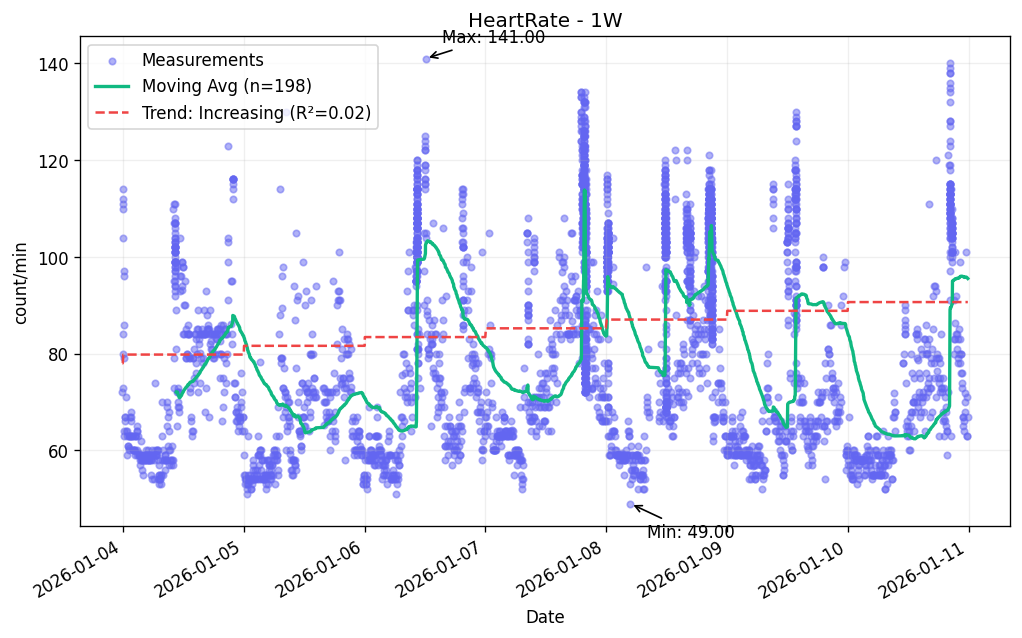
\includegraphics[width=0.95\textwidth]{plots_medical/Cardiovascular/heartrate_1W.png}
\end{figure}
\begin{figure}[H]
\centering
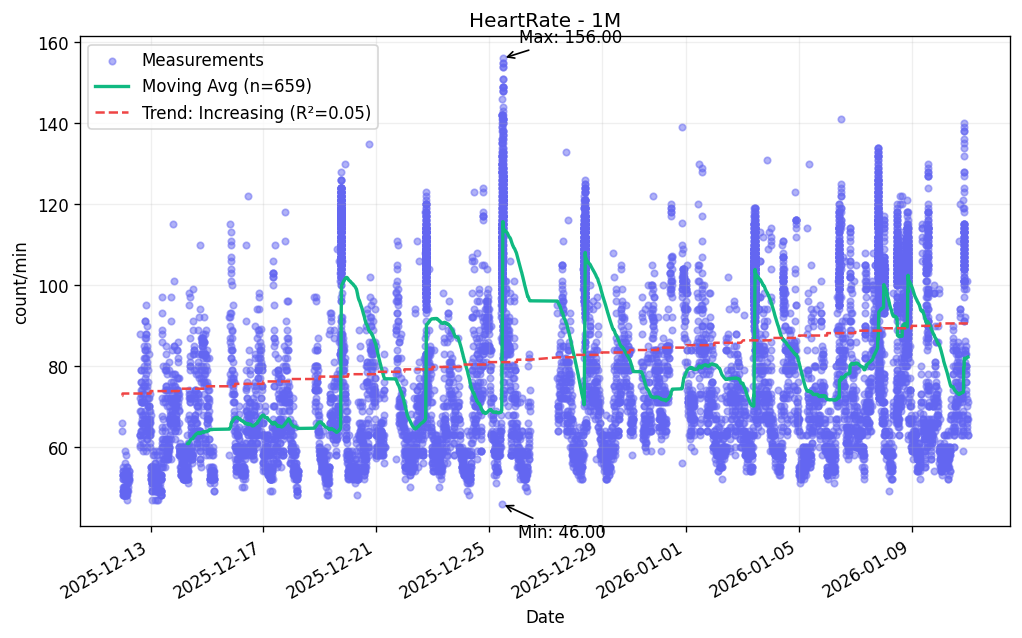
\includegraphics[width=0.95\textwidth]{plots_medical/Cardiovascular/heartrate_1M.png}
\end{figure}
\begin{figure}[H]
\centering
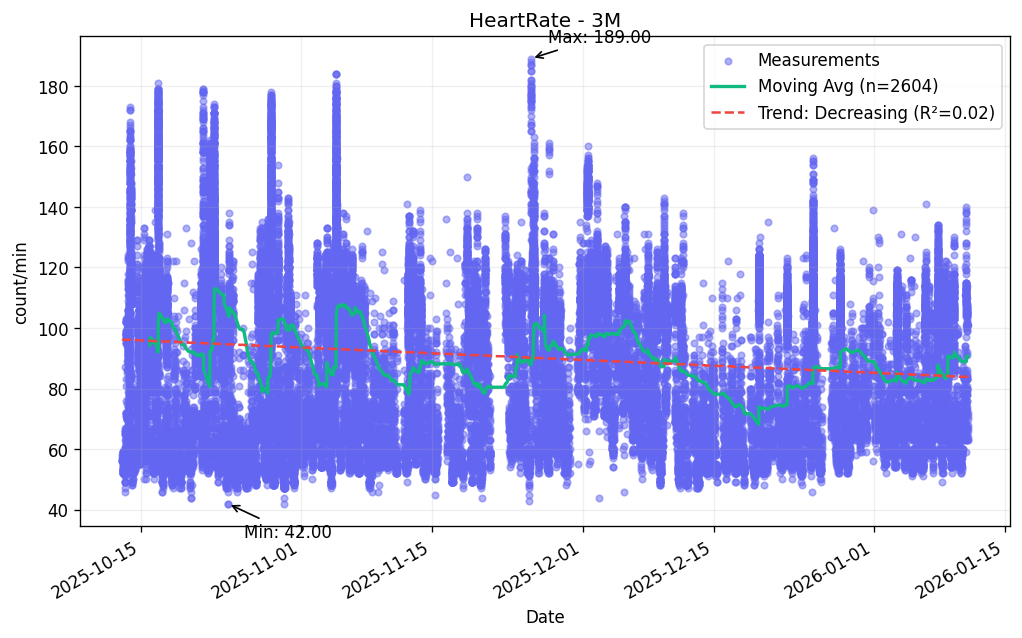
\includegraphics[width=0.95\textwidth]{plots_medical/Cardiovascular/heartrate_3M.png}
\end{figure}
\begin{figure}[H]
\centering
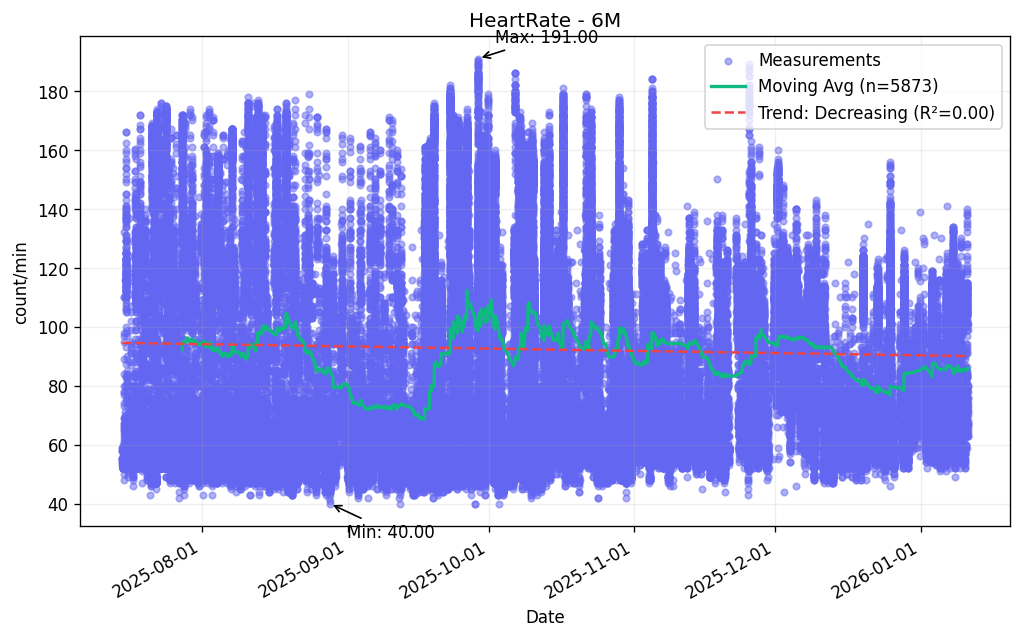
\includegraphics[width=0.95\textwidth]{plots_medical/Cardiovascular/heartrate_6M.png}
\end{figure}
\begin{figure}[H]
\centering
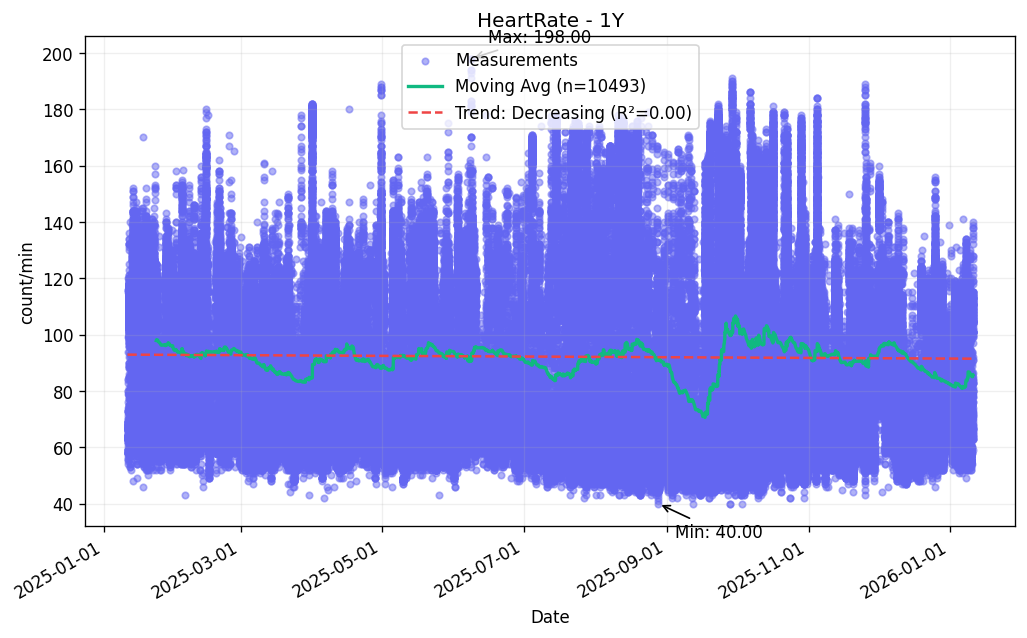
\includegraphics[width=0.95\textwidth]{plots_medical/Cardiovascular/heartrate_1Y.png}
\end{figure}
\begin{figure}[H]
\centering
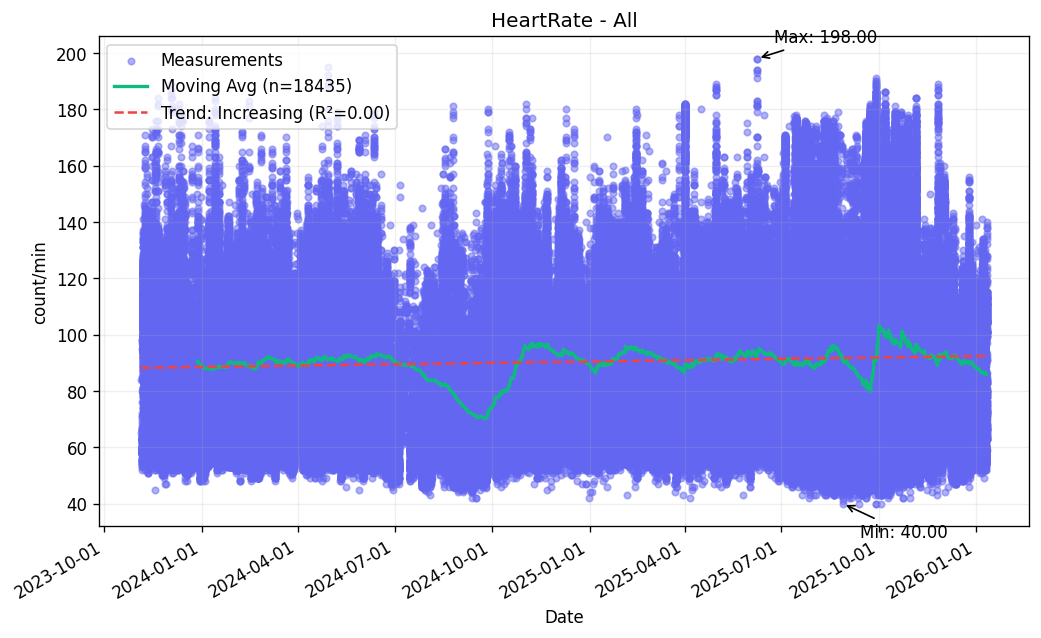
\includegraphics[width=0.95\textwidth]{plots_medical/Cardiovascular/heartrate_All.png}
\end{figure}
\clearpage
\subsection{HeartRateRecoveryOneMinute}
\begin{table}[H]
\centering
\resizebox{\textwidth}{!}{
\begin{tabular}{|l|c|c|c|c|c|c|}
\hline
\textbf{Window} & \textbf{Min} & \textbf{Max} & \textbf{Avg} & \textbf{Start} & \textbf{End} & \textbf{Trend Slope} \\ \hline
1W & 28.10 count/min & 31.70 count/min & 29.24 count/min & 28.57 & 31.70 & 0.41366 \\ \hline
1M & 28.10 count/min & 38.47 count/min & 32.45 count/min & 38.40 & 31.70 & -0.48453 \\ \hline
3M & 28.10 count/min & 46.32 count/min & 39.39 count/min & 46.32 & 31.70 & -0.17819 \\ \hline
6M & 18.92 count/min & 46.32 count/min & 38.97 count/min & 18.92 & 31.70 & -0.03657 \\ \hline
1Y & 18.92 count/min & 46.32 count/min & 33.89 count/min & 33.12 & 31.70 & 0.02975 \\ \hline
All & 18.65 count/min & 46.32 count/min & 32.98 count/min & 32.64 & 31.70 & 0.01559 \\ \hline
\end{tabular}
}
\caption{Detailed Statistics for HeartRateRecoveryOneMinute}
\end{table}
\begin{figure}[H]
\centering
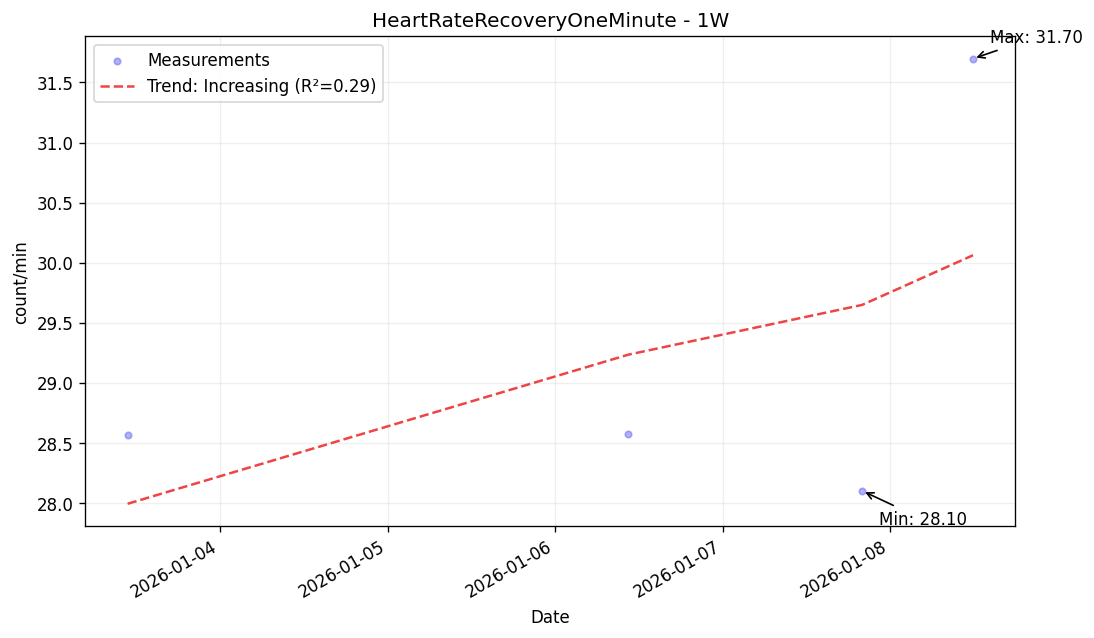
\includegraphics[width=0.95\textwidth]{plots_medical/Cardiovascular/heartraterecoveryoneminute_1W.png}
\end{figure}
\begin{figure}[H]
\centering
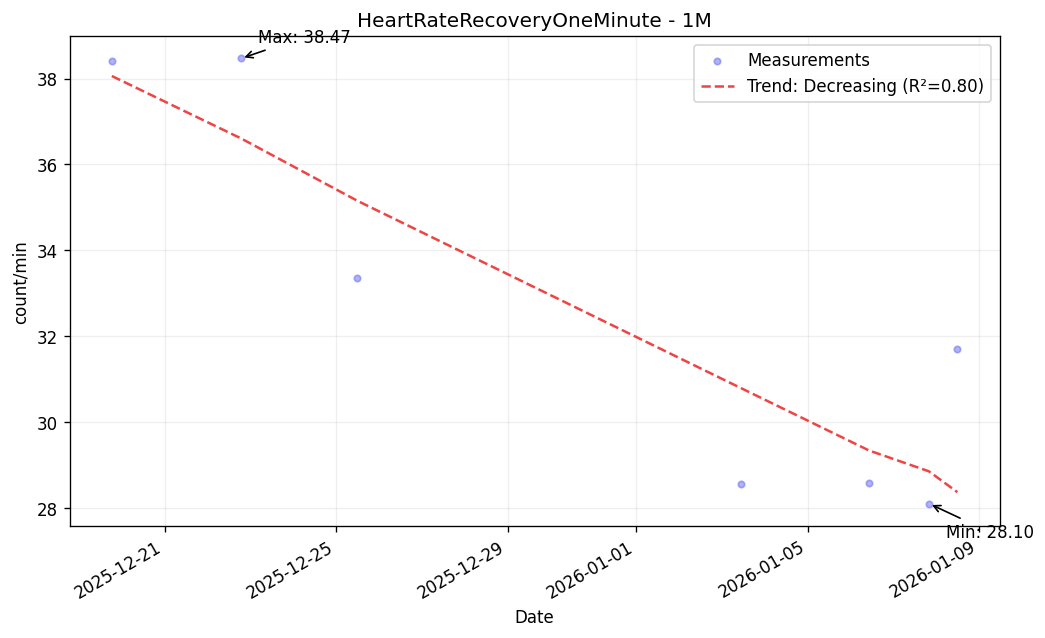
\includegraphics[width=0.95\textwidth]{plots_medical/Cardiovascular/heartraterecoveryoneminute_1M.png}
\end{figure}
\begin{figure}[H]
\centering
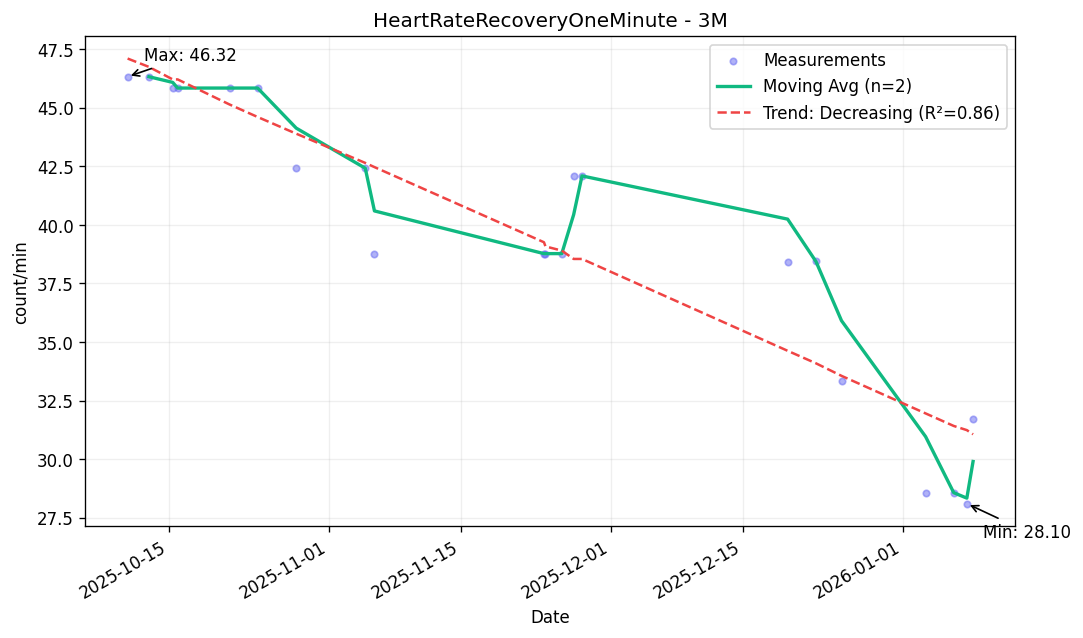
\includegraphics[width=0.95\textwidth]{plots_medical/Cardiovascular/heartraterecoveryoneminute_3M.png}
\end{figure}
\begin{figure}[H]
\centering
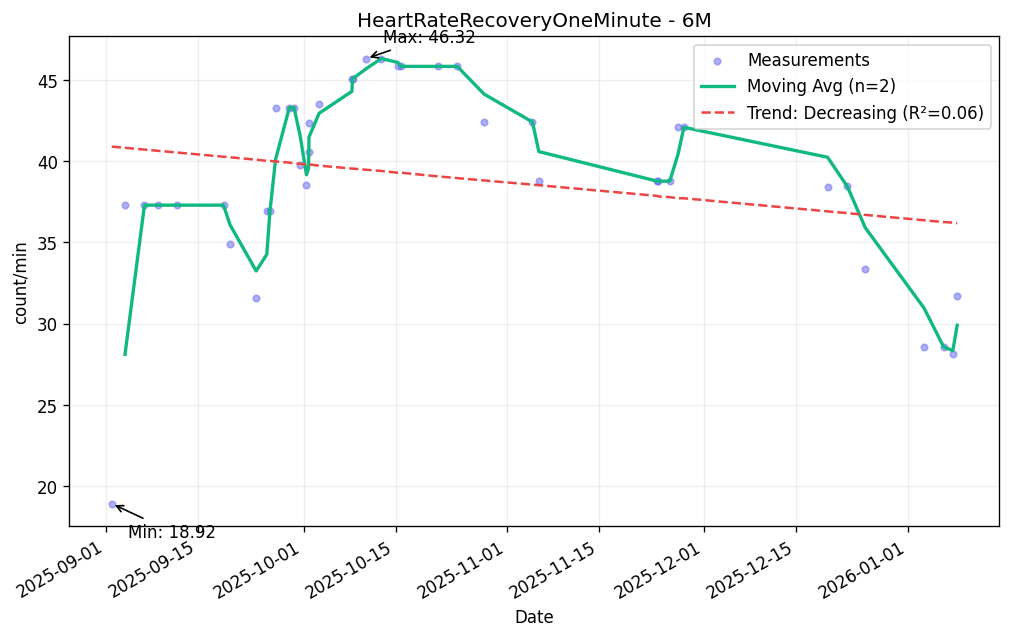
\includegraphics[width=0.95\textwidth]{plots_medical/Cardiovascular/heartraterecoveryoneminute_6M.png}
\end{figure}
\begin{figure}[H]
\centering
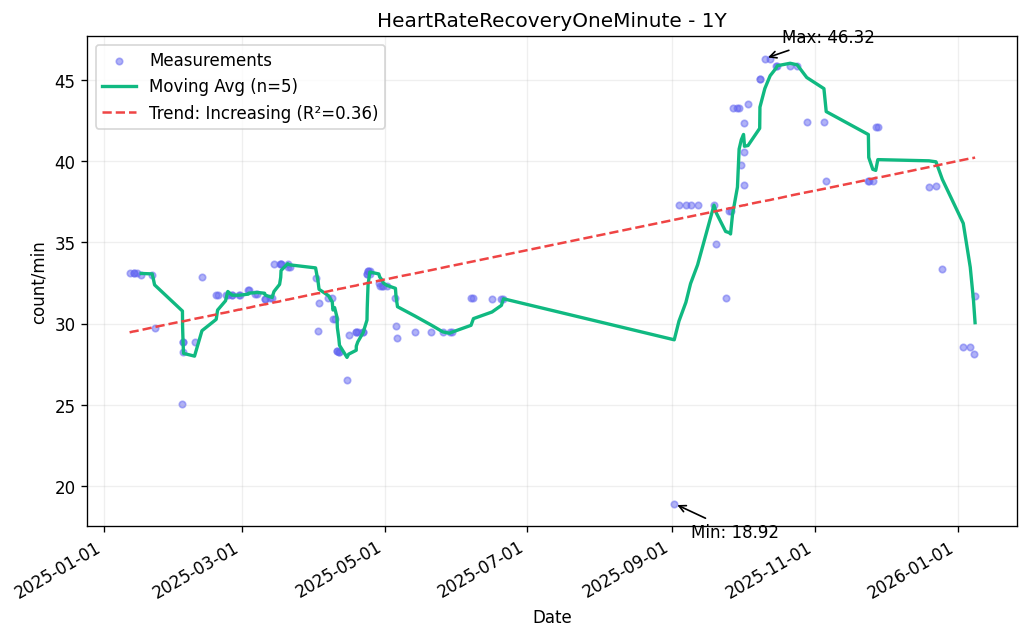
\includegraphics[width=0.95\textwidth]{plots_medical/Cardiovascular/heartraterecoveryoneminute_1Y.png}
\end{figure}
\begin{figure}[H]
\centering
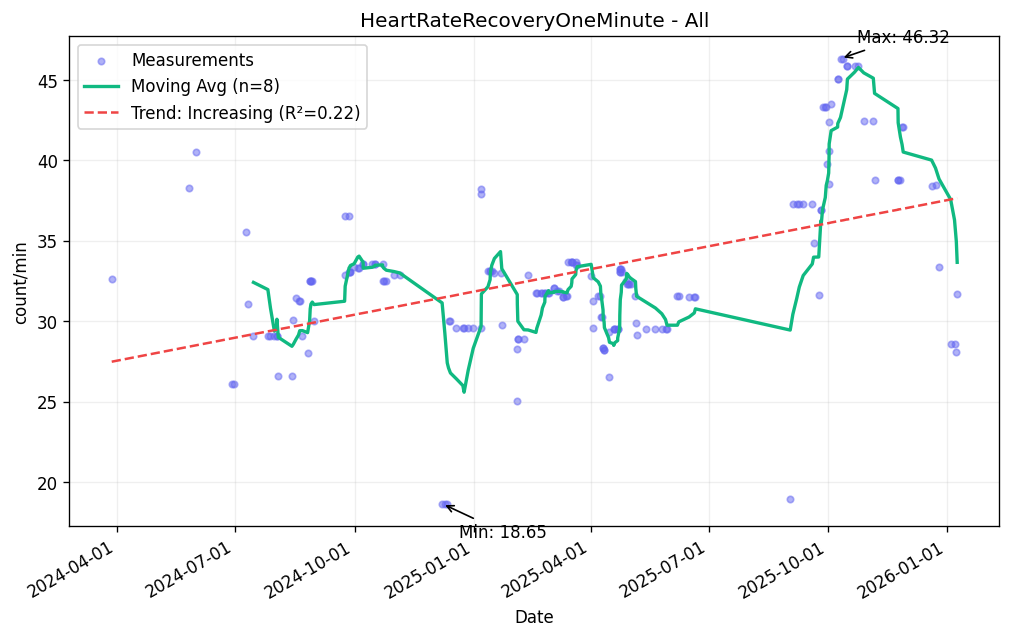
\includegraphics[width=0.95\textwidth]{plots_medical/Cardiovascular/heartraterecoveryoneminute_All.png}
\end{figure}
\clearpage
\subsection{HeartRateVariabilitySDNN}
\begin{table}[H]
\centering
\resizebox{\textwidth}{!}{
\begin{tabular}{|l|c|c|c|c|c|c|}
\hline
\textbf{Window} & \textbf{Min} & \textbf{Max} & \textbf{Avg} & \textbf{Start} & \textbf{End} & \textbf{Trend Slope} \\ \hline
1W & 21.49 ms & 190.34 ms & 60.53 ms & 125.22 & 90.85 & 2.47894 \\ \hline
1M & 13.21 ms & 194.14 ms & 60.79 ms & 50.21 & 90.85 & -0.18927 \\ \hline
3M & 10.82 ms & 217.98 ms & 60.71 ms & 34.82 & 90.85 & -0.12134 \\ \hline
6M & 10.82 ms & 245.75 ms & 65.81 ms & 68.18 & 90.85 & -0.09805 \\ \hline
1Y & 10.82 ms & 248.71 ms & 62.16 ms & 70.61 & 90.85 & 0.01771 \\ \hline
All & 6.03 ms & 274.62 ms & 60.46 ms & 77.25 & 90.85 & 0.00927 \\ \hline
\end{tabular}
}
\caption{Detailed Statistics for HeartRateVariabilitySDNN}
\end{table}
\begin{figure}[H]
\centering
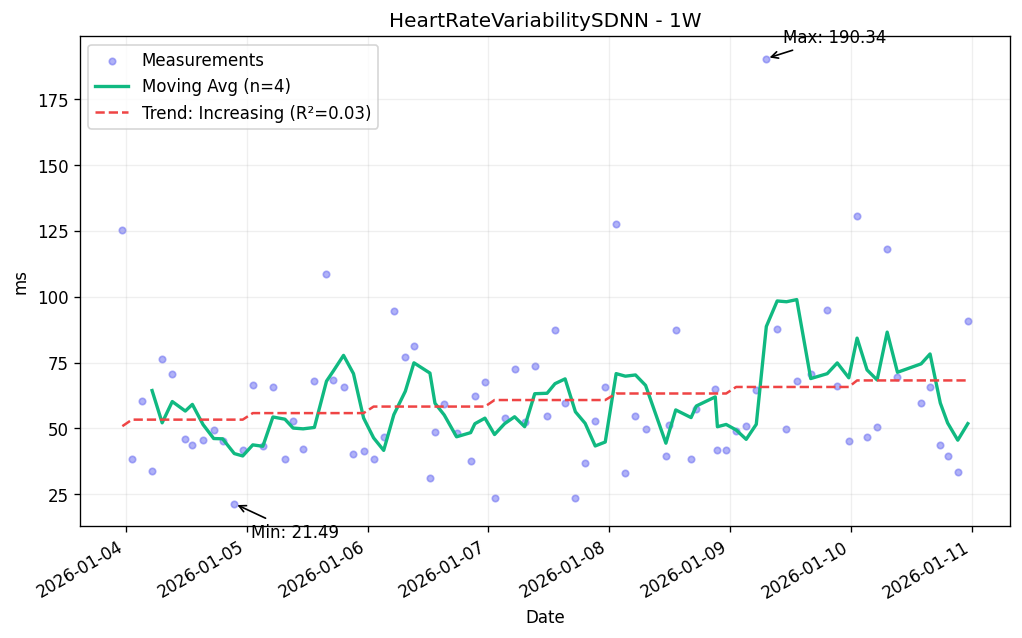
\includegraphics[width=0.95\textwidth]{plots_medical/Cardiovascular/heartratevariabilitysdnn_1W.png}
\end{figure}
\begin{figure}[H]
\centering
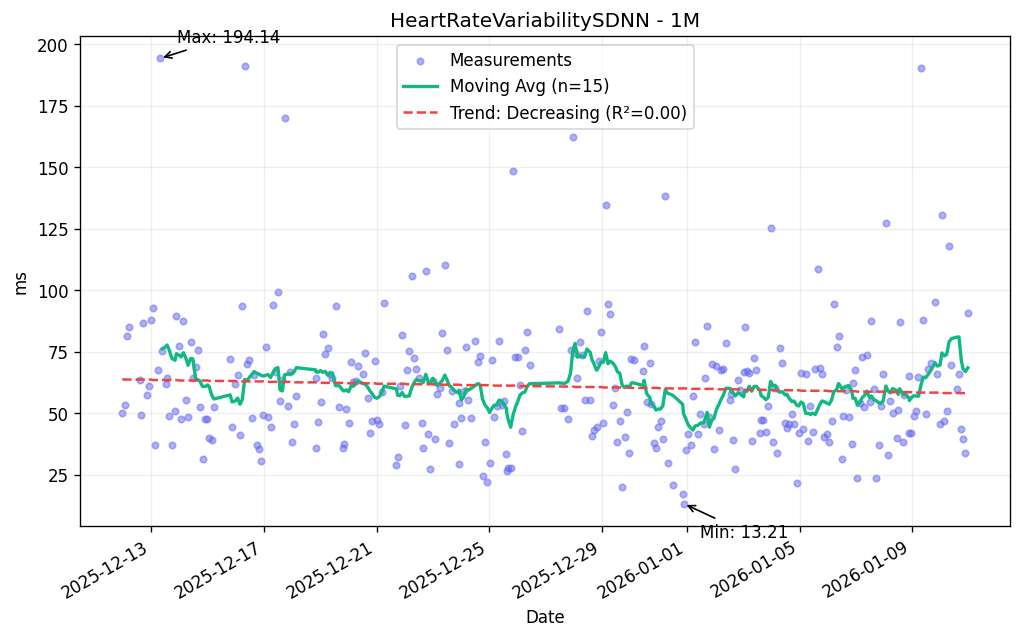
\includegraphics[width=0.95\textwidth]{plots_medical/Cardiovascular/heartratevariabilitysdnn_1M.png}
\end{figure}
\begin{figure}[H]
\centering
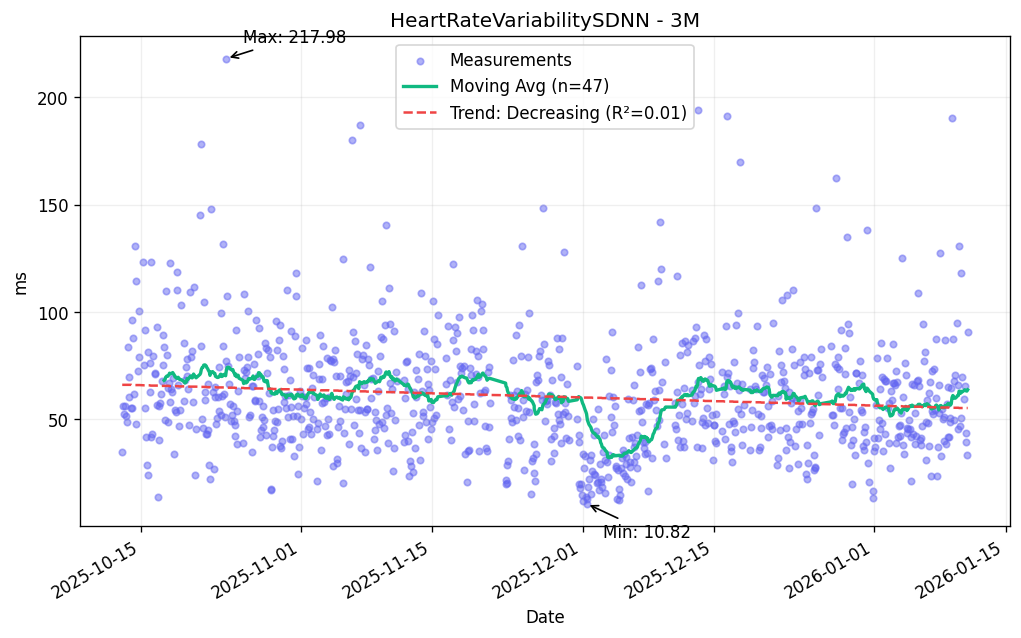
\includegraphics[width=0.95\textwidth]{plots_medical/Cardiovascular/heartratevariabilitysdnn_3M.png}
\end{figure}
\begin{figure}[H]
\centering
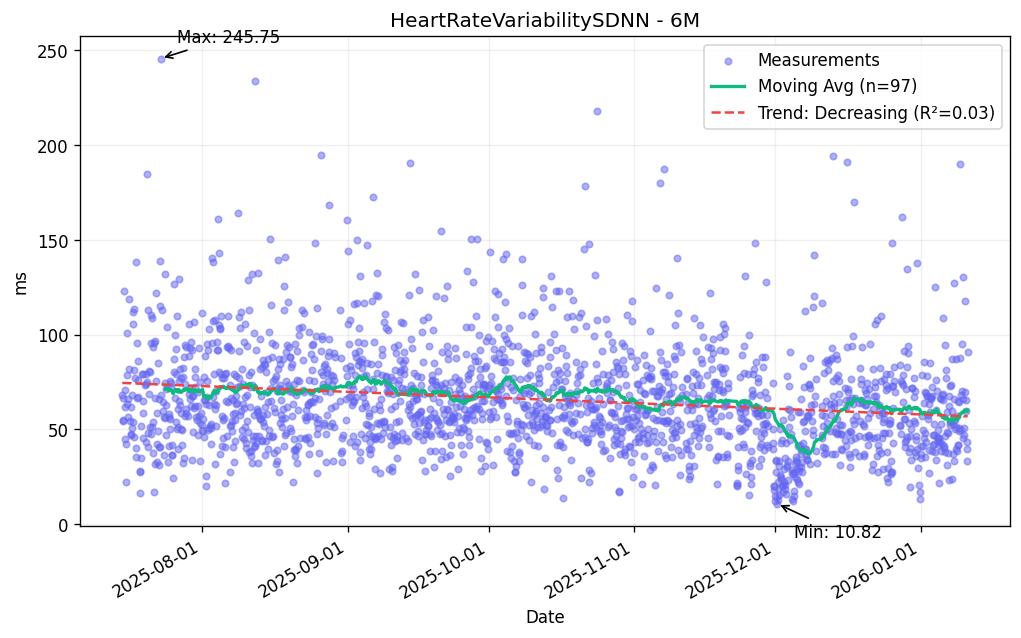
\includegraphics[width=0.95\textwidth]{plots_medical/Cardiovascular/heartratevariabilitysdnn_6M.png}
\end{figure}
\begin{figure}[H]
\centering
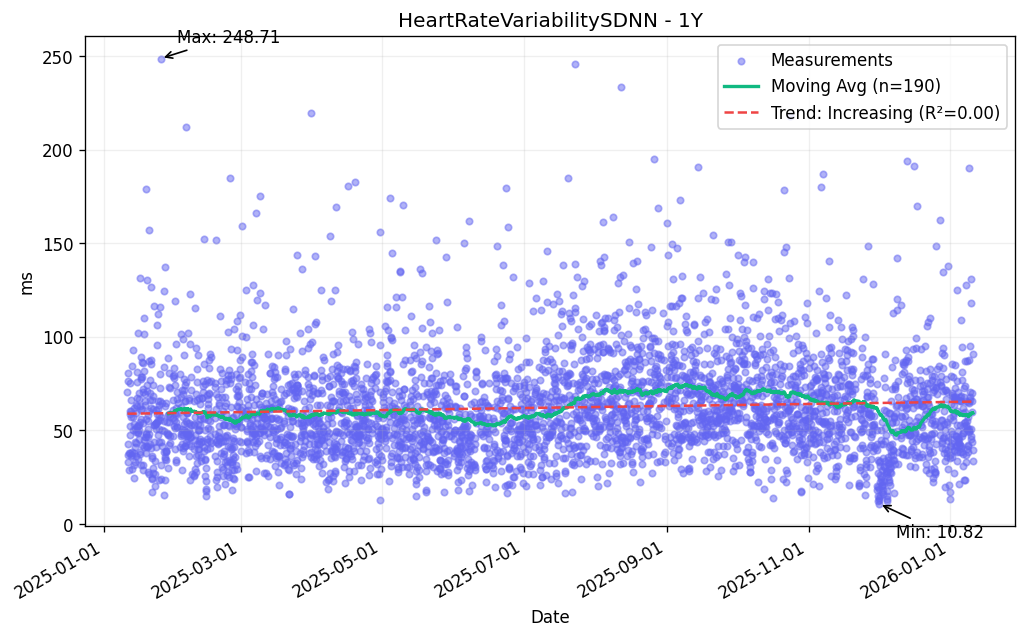
\includegraphics[width=0.95\textwidth]{plots_medical/Cardiovascular/heartratevariabilitysdnn_1Y.png}
\end{figure}
\begin{figure}[H]
\centering
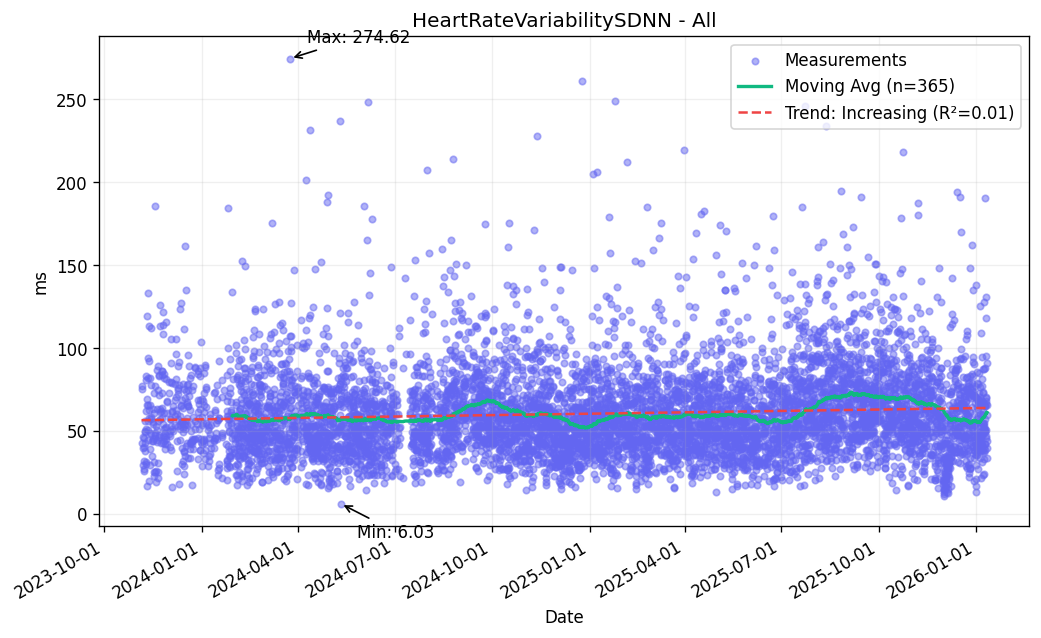
\includegraphics[width=0.95\textwidth]{plots_medical/Cardiovascular/heartratevariabilitysdnn_All.png}
\end{figure}
\clearpage
\subsection{RestingHeartRate}
\begin{table}[H]
\centering
\resizebox{\textwidth}{!}{
\begin{tabular}{|l|c|c|c|c|c|c|}
\hline
\textbf{Window} & \textbf{Min} & \textbf{Max} & \textbf{Avg} & \textbf{Start} & \textbf{End} & \textbf{Trend Slope} \\ \hline
1W & 58.00 count/min & 65.00 count/min & 60.38 count/min & 63.00 & 59.00 & -0.17857 \\ \hline
1M & 54.00 count/min & 72.00 count/min & 59.47 count/min & 60.00 & 59.00 & 0.15288 \\ \hline
3M & 49.00 count/min & 96.00 count/min & 60.36 count/min & 57.00 & 59.00 & 0.05492 \\ \hline
6M & 47.00 count/min & 96.00 count/min & 57.30 count/min & 57.00 & 59.00 & 0.05448 \\ \hline
1Y & 47.00 count/min & 96.00 count/min & 59.17 count/min & 63.00 & 59.00 & -0.00912 \\ \hline
All & 47.00 count/min & 96.00 count/min & 59.65 count/min & 64.00 & 59.00 & -0.00250 \\ \hline
\end{tabular}
}
\caption{Detailed Statistics for RestingHeartRate}
\end{table}
\begin{figure}[H]
\centering
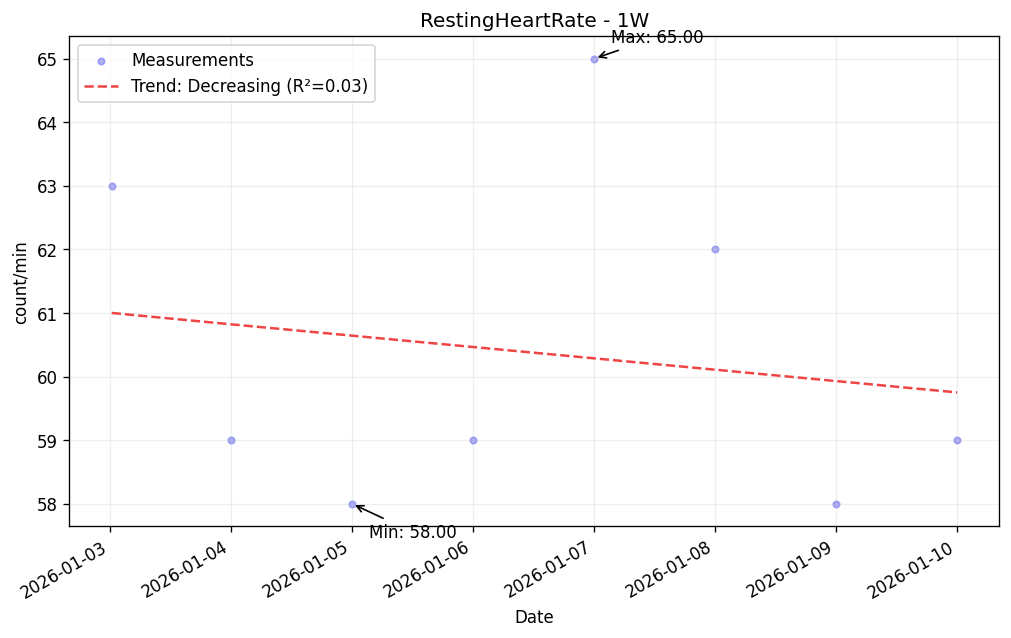
\includegraphics[width=0.95\textwidth]{plots_medical/Cardiovascular/restingheartrate_1W.png}
\end{figure}
\begin{figure}[H]
\centering
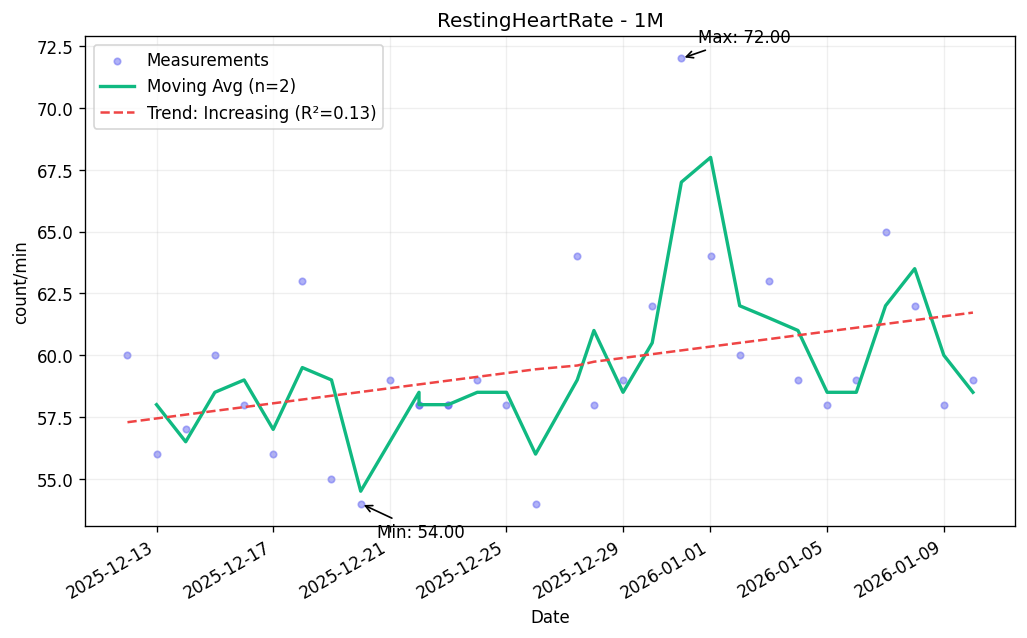
\includegraphics[width=0.95\textwidth]{plots_medical/Cardiovascular/restingheartrate_1M.png}
\end{figure}
\begin{figure}[H]
\centering
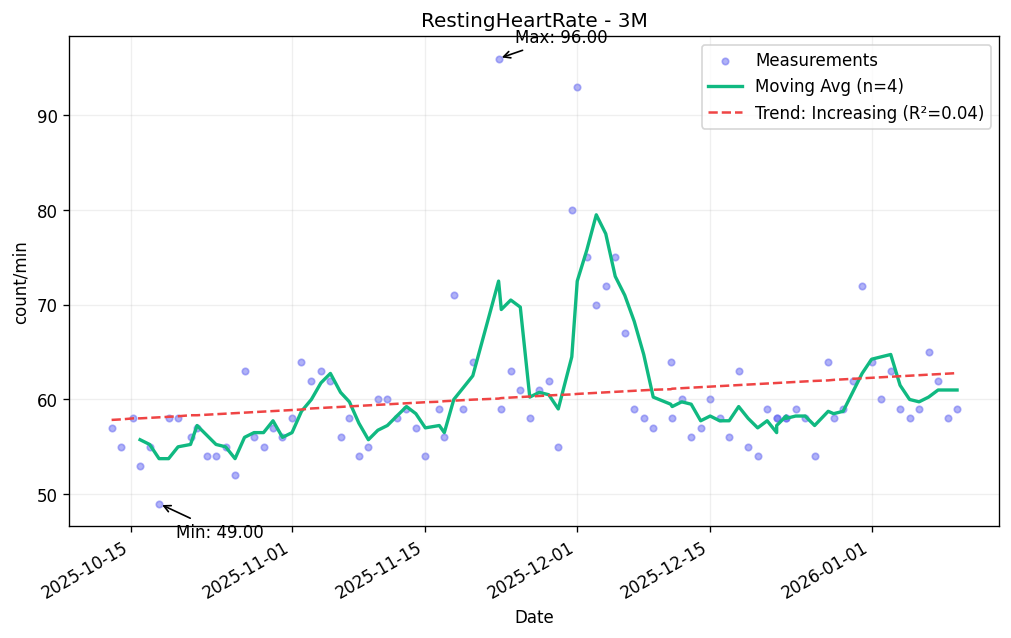
\includegraphics[width=0.95\textwidth]{plots_medical/Cardiovascular/restingheartrate_3M.png}
\end{figure}
\begin{figure}[H]
\centering
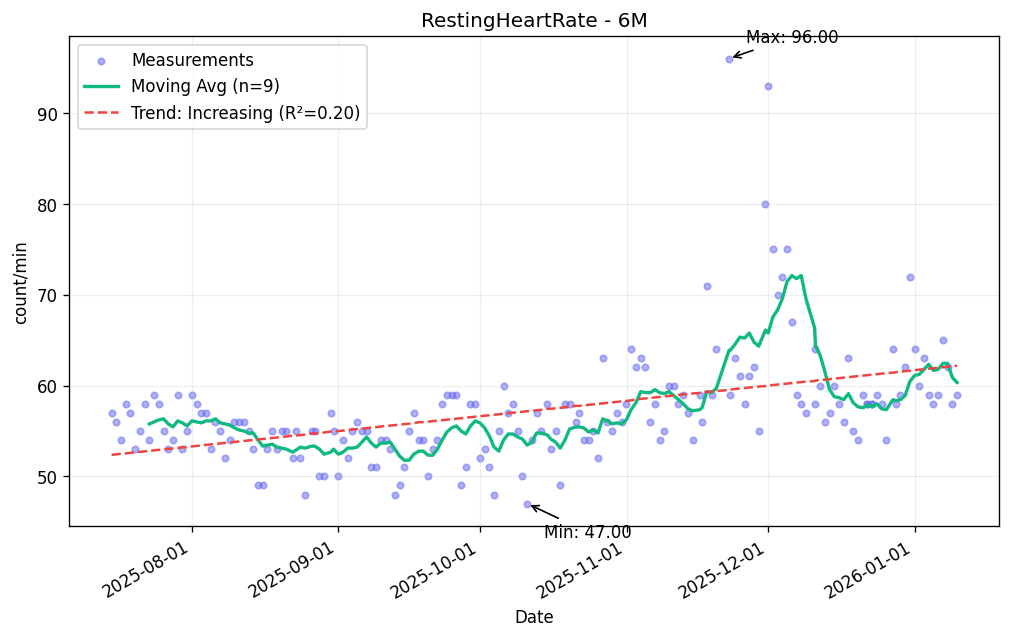
\includegraphics[width=0.95\textwidth]{plots_medical/Cardiovascular/restingheartrate_6M.png}
\end{figure}
\begin{figure}[H]
\centering
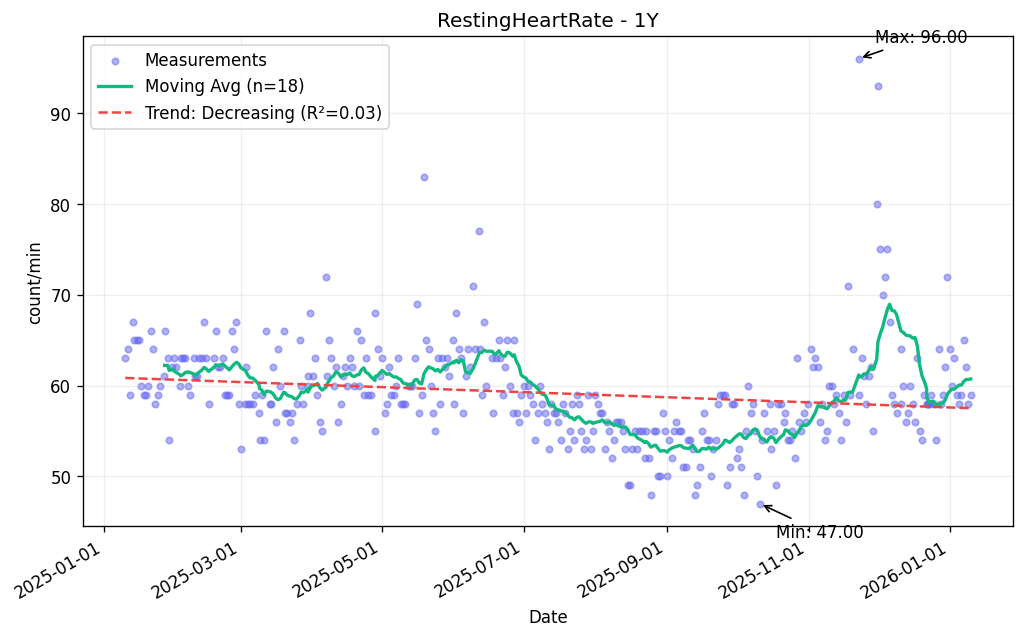
\includegraphics[width=0.95\textwidth]{plots_medical/Cardiovascular/restingheartrate_1Y.png}
\end{figure}
\begin{figure}[H]
\centering
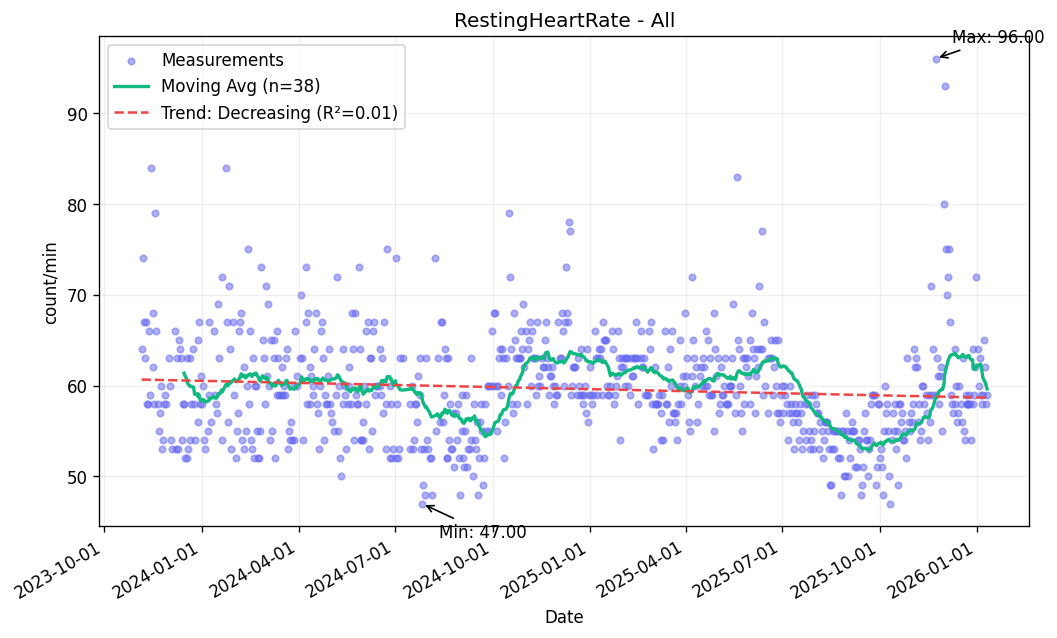
\includegraphics[width=0.95\textwidth]{plots_medical/Cardiovascular/restingheartrate_All.png}
\end{figure}
\clearpage
\subsection{VO2Max}
\begin{table}[H]
\centering
\resizebox{\textwidth}{!}{
\begin{tabular}{|l|c|c|c|c|c|c|}
\hline
\textbf{Window} & \textbf{Min} & \textbf{Max} & \textbf{Avg} & \textbf{Start} & \textbf{End} & \textbf{Trend Slope} \\ \hline
1W & 35.99 mL/min·kg & 36.68 mL/min·kg & 36.31 mL/min·kg & 36.68 & 36.54 & 0.00432 \\ \hline
1M & 34.63 mL/min·kg & 36.68 mL/min·kg & 35.90 mL/min·kg & 34.83 & 36.54 & 0.07865 \\ \hline
3M & 34.63 mL/min·kg & 39.87 mL/min·kg & 37.31 mL/min·kg & 38.88 & 36.54 & -0.04507 \\ \hline
6M & 34.63 mL/min·kg & 41.06 mL/min·kg & 37.94 mL/min·kg & 35.73 & 36.54 & -0.02412 \\ \hline
1Y & 32.47 mL/min·kg & 41.06 mL/min·kg & 34.94 mL/min·kg & 34.51 & 36.54 & 0.01728 \\ \hline
All & 32.47 mL/min·kg & 41.25 mL/min·kg & 35.08 mL/min·kg & 41.25 & 36.54 & 0.00109 \\ \hline
\end{tabular}
}
\caption{Detailed Statistics for VO2Max}
\end{table}
\begin{figure}[H]
\centering
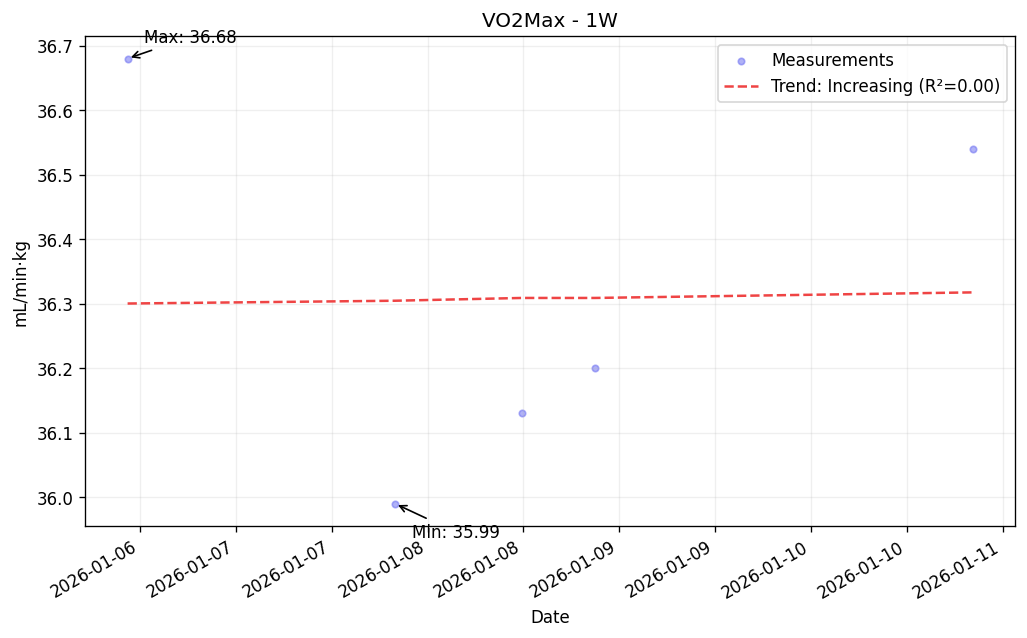
\includegraphics[width=0.95\textwidth]{plots_medical/Cardiovascular/vo2max_1W.png}
\end{figure}
\begin{figure}[H]
\centering
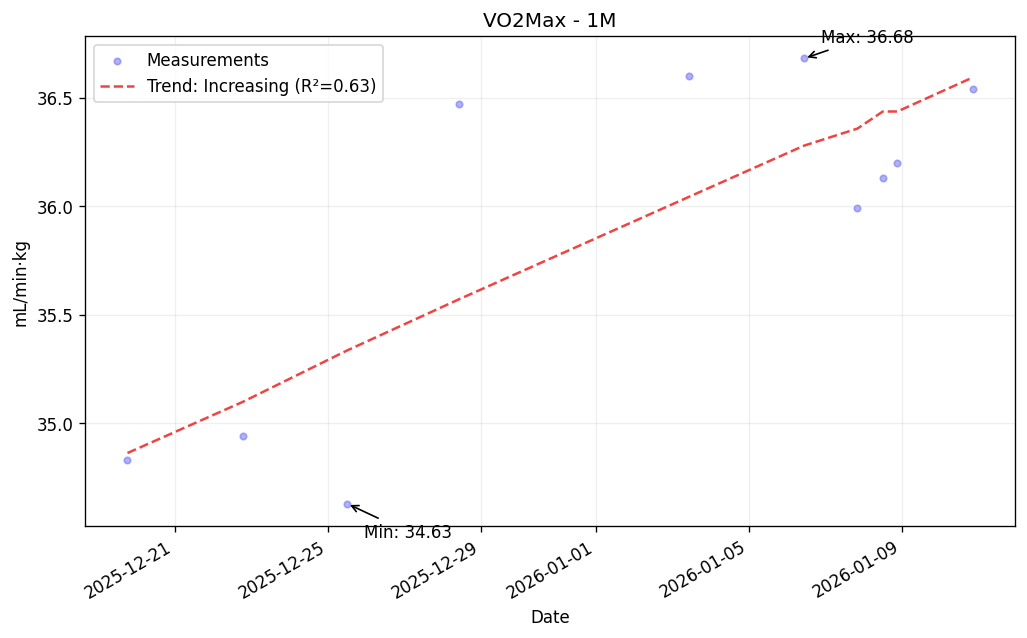
\includegraphics[width=0.95\textwidth]{plots_medical/Cardiovascular/vo2max_1M.png}
\end{figure}
\begin{figure}[H]
\centering
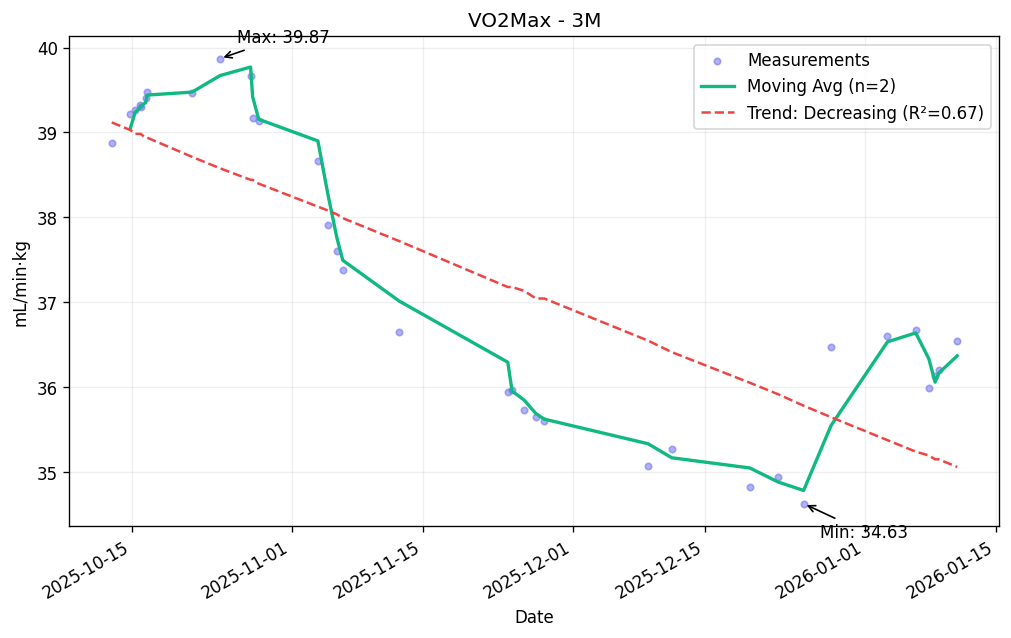
\includegraphics[width=0.95\textwidth]{plots_medical/Cardiovascular/vo2max_3M.png}
\end{figure}
\begin{figure}[H]
\centering
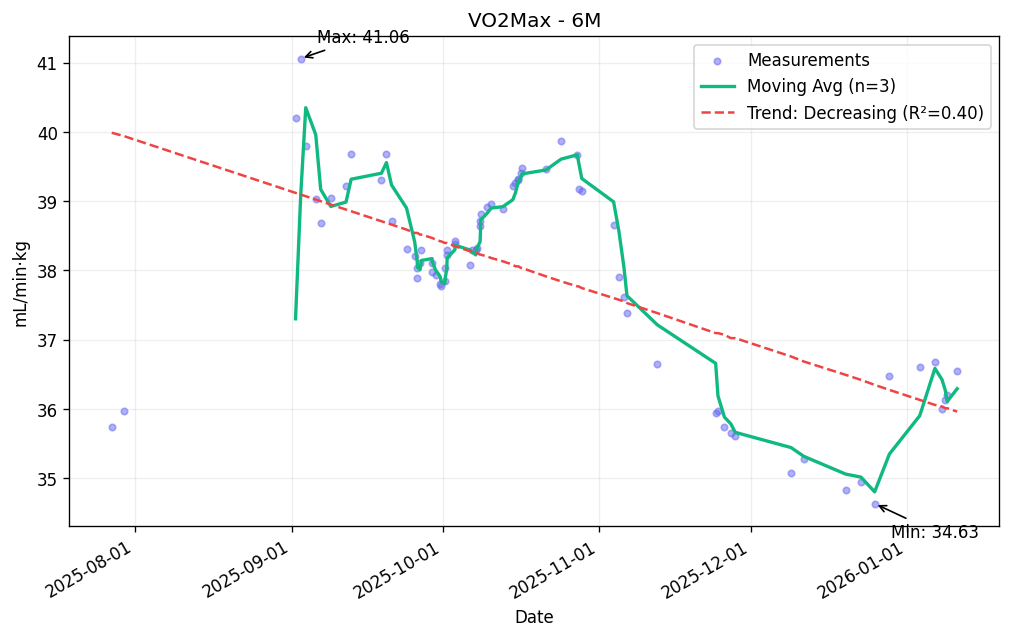
\includegraphics[width=0.95\textwidth]{plots_medical/Cardiovascular/vo2max_6M.png}
\end{figure}
\begin{figure}[H]
\centering
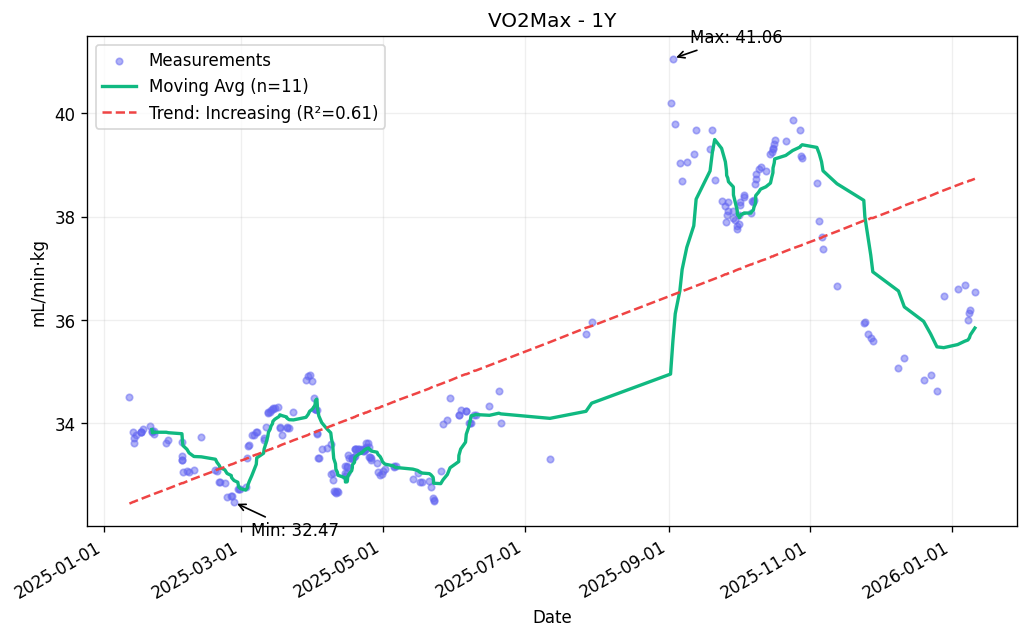
\includegraphics[width=0.95\textwidth]{plots_medical/Cardiovascular/vo2max_1Y.png}
\end{figure}
\begin{figure}[H]
\centering
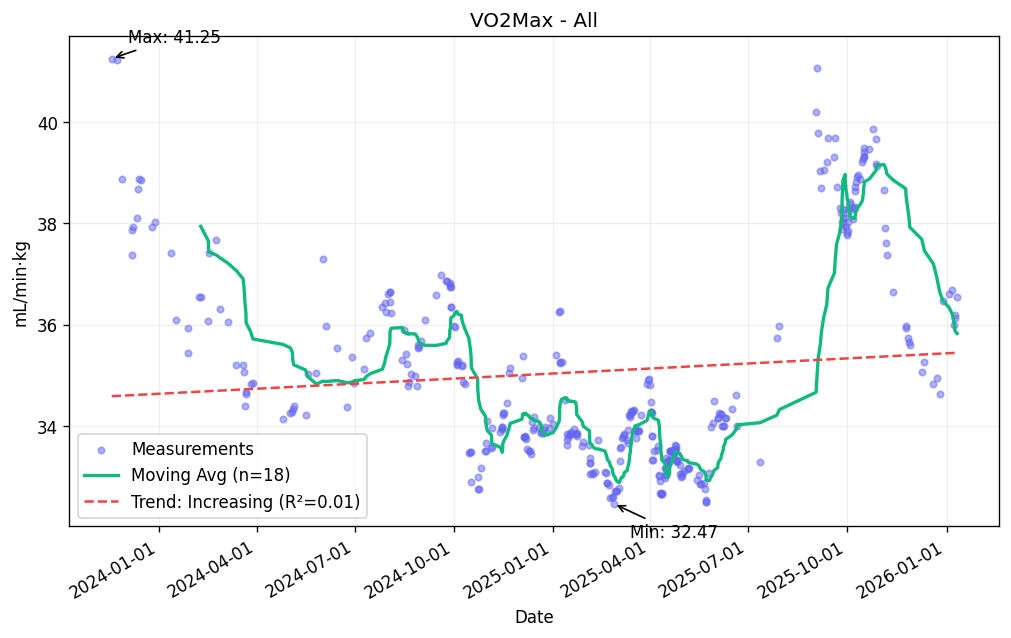
\includegraphics[width=0.95\textwidth]{plots_medical/Cardiovascular/vo2max_All.png}
\end{figure}
\clearpage
\subsection{WalkingHeartRateAverage}
\begin{table}[H]
\centering
\resizebox{\textwidth}{!}{
\begin{tabular}{|l|c|c|c|c|c|c|}
\hline
\textbf{Window} & \textbf{Min} & \textbf{Max} & \textbf{Avg} & \textbf{Start} & \textbf{End} & \textbf{Trend Slope} \\ \hline
1W & 97.00 count/min & 110.50 count/min & 104.21 count/min & 102.00 & 110.50 & 1.34221 \\ \hline
1M & 88.00 count/min & 139.00 count/min & 103.76 count/min & 90.00 & 110.50 & 0.37365 \\ \hline
3M & 85.00 count/min & 154.00 count/min & 105.17 count/min & 100.50 & 110.50 & 0.01395 \\ \hline
6M & 80.00 count/min & 174.00 count/min & 117.59 count/min & 156.00 & 110.50 & -0.26615 \\ \hline
1Y & 80.00 count/min & 174.00 count/min & 115.38 count/min & 108.00 & 110.50 & -0.00850 \\ \hline
All & 68.00 count/min & 174.00 count/min & 111.10 count/min & 111.00 & 110.50 & 0.01519 \\ \hline
\end{tabular}
}
\caption{Detailed Statistics for WalkingHeartRateAverage}
\end{table}
\begin{figure}[H]
\centering
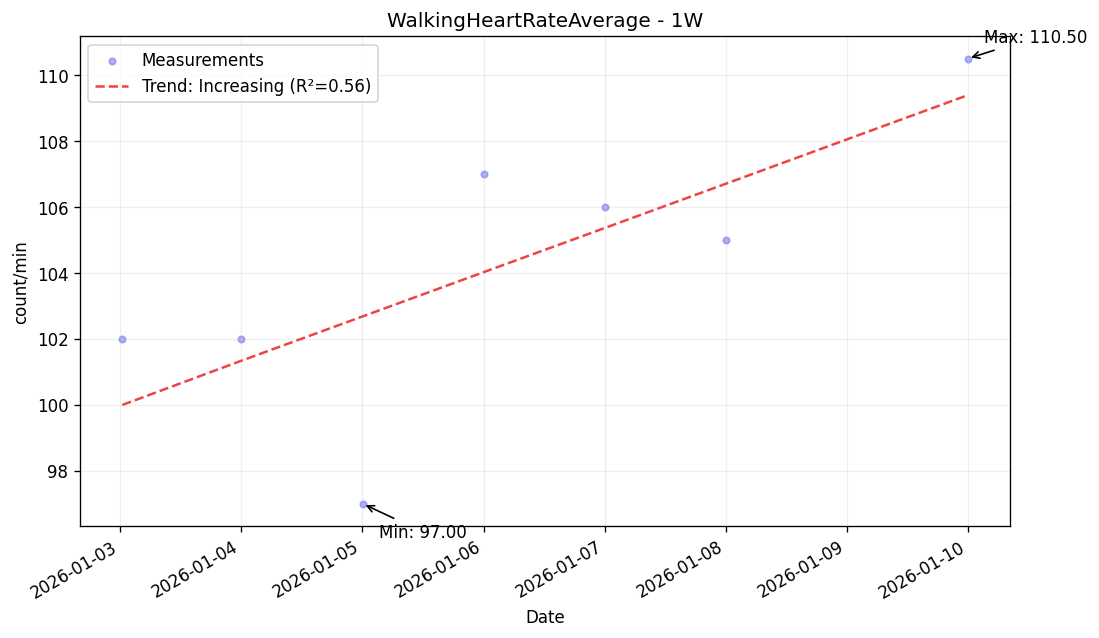
\includegraphics[width=0.95\textwidth]{plots_medical/Cardiovascular/walkingheartrateaverage_1W.png}
\end{figure}
\begin{figure}[H]
\centering
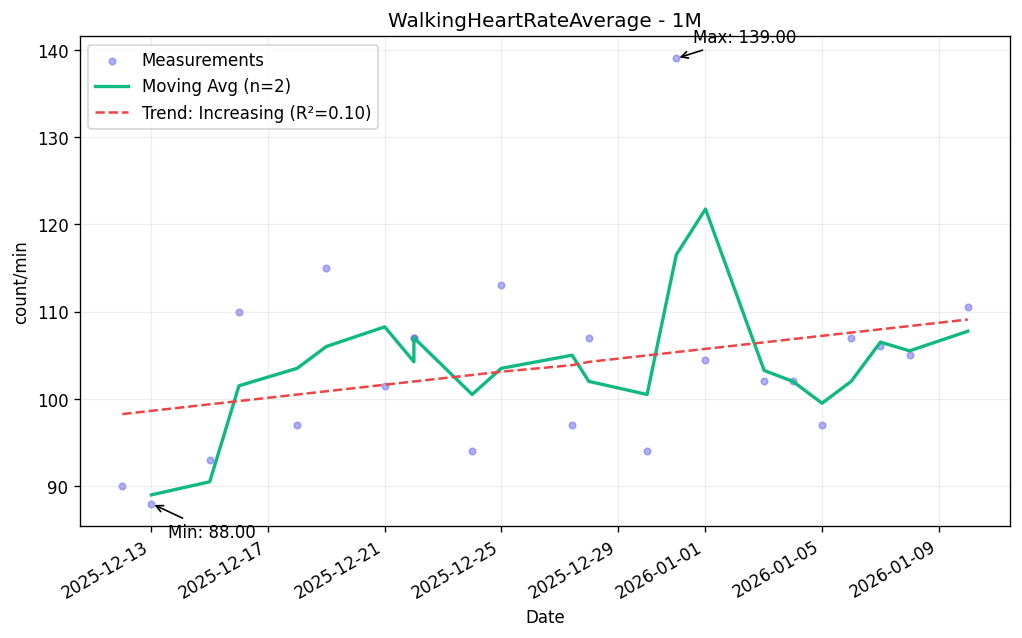
\includegraphics[width=0.95\textwidth]{plots_medical/Cardiovascular/walkingheartrateaverage_1M.png}
\end{figure}
\begin{figure}[H]
\centering
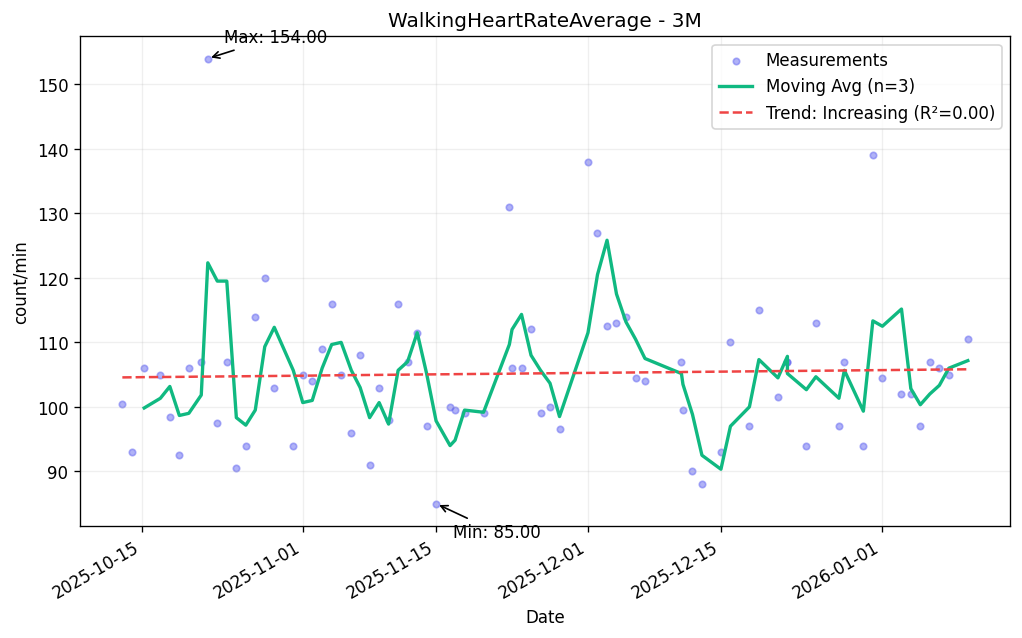
\includegraphics[width=0.95\textwidth]{plots_medical/Cardiovascular/walkingheartrateaverage_3M.png}
\end{figure}
\begin{figure}[H]
\centering
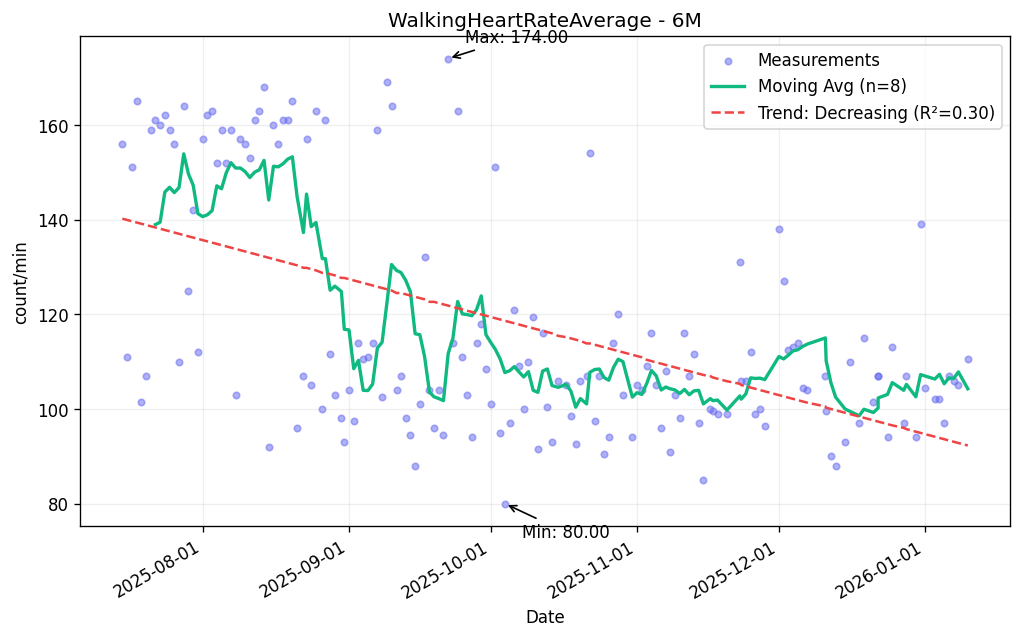
\includegraphics[width=0.95\textwidth]{plots_medical/Cardiovascular/walkingheartrateaverage_6M.png}
\end{figure}
\begin{figure}[H]
\centering
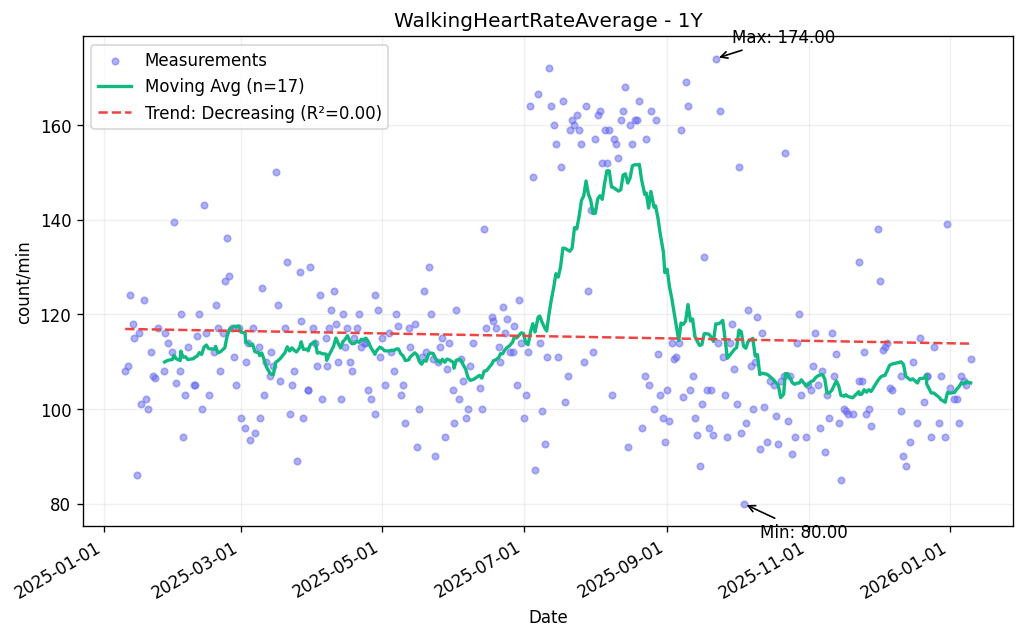
\includegraphics[width=0.95\textwidth]{plots_medical/Cardiovascular/walkingheartrateaverage_1Y.png}
\end{figure}
\begin{figure}[H]
\centering
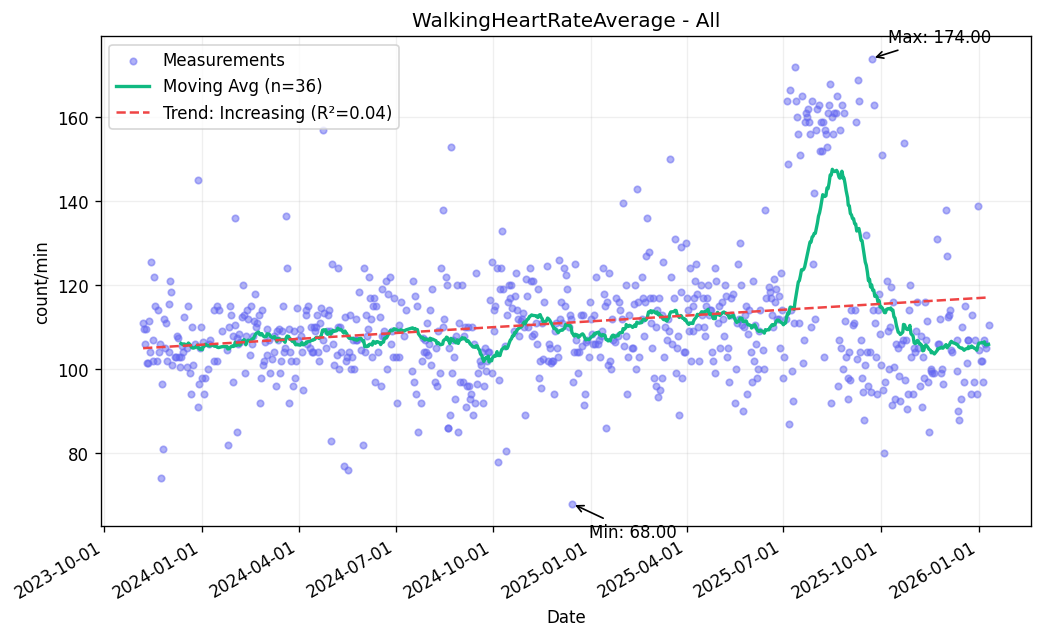
\includegraphics[width=0.95\textwidth]{plots_medical/Cardiovascular/walkingheartrateaverage_All.png}
\end{figure}
\clearpage
\section{Respiratory}
\subsection{OxygenSaturation}
\begin{table}[H]
\centering
\resizebox{\textwidth}{!}{
\begin{tabular}{|l|c|c|c|c|c|c|}
\hline
\textbf{Window} & \textbf{Min} & \textbf{Max} & \textbf{Avg} & \textbf{Start} & \textbf{End} & \textbf{Trend Slope} \\ \hline
1W & 0.87 \% & 1.00 \% & 0.96 \% & 0.99 & 0.96 & -0.00103 \\ \hline
1M & 0.87 \% & 1.00 \% & 0.97 \% & 0.96 & 0.96 & -0.00013 \\ \hline
3M & 0.85 \% & 1.00 \% & 0.96 \% & 0.93 & 0.96 & -0.00004 \\ \hline
6M & 0.83 \% & 1.00 \% & 0.96 \% & 0.96 & 0.96 & -0.00001 \\ \hline
1Y & 0.83 \% & 1.00 \% & 0.96 \% & 0.96 & 0.96 & -0.00001 \\ \hline
All & 0.82 \% & 1.00 \% & 0.97 \% & 0.95 & 0.96 & -0.00002 \\ \hline
\end{tabular}
}
\caption{Detailed Statistics for OxygenSaturation}
\end{table}
\begin{figure}[H]
\centering
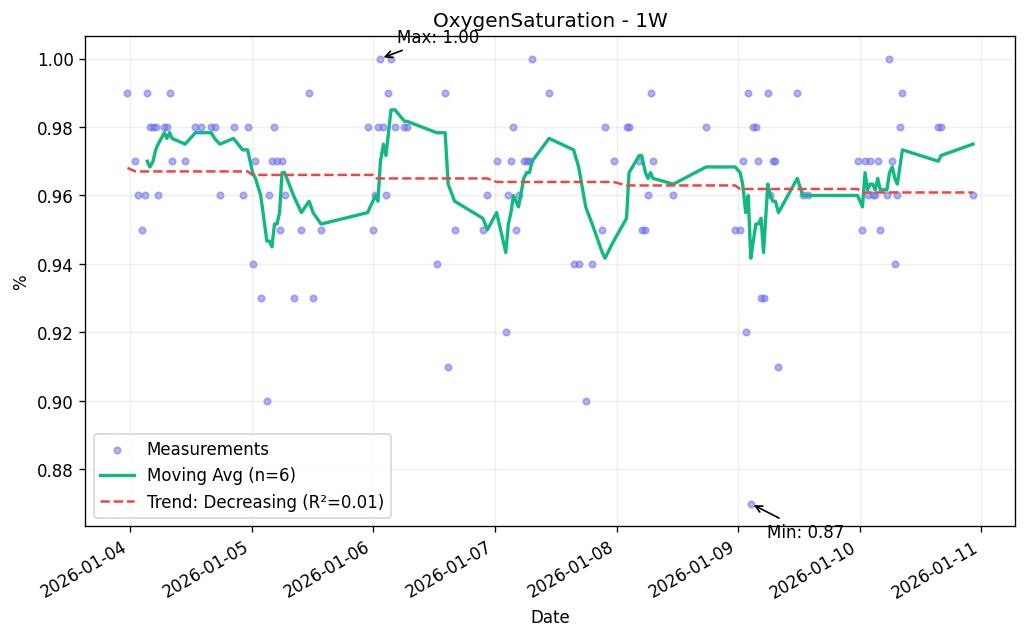
\includegraphics[width=0.95\textwidth]{plots_medical/Respiratory/oxygensaturation_1W.png}
\end{figure}
\begin{figure}[H]
\centering
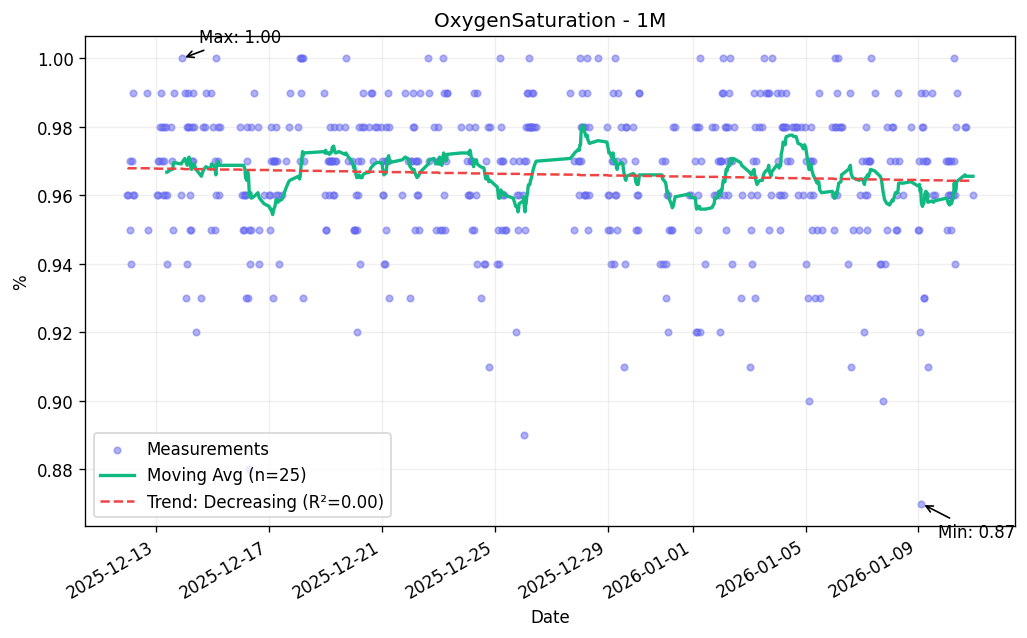
\includegraphics[width=0.95\textwidth]{plots_medical/Respiratory/oxygensaturation_1M.png}
\end{figure}
\begin{figure}[H]
\centering
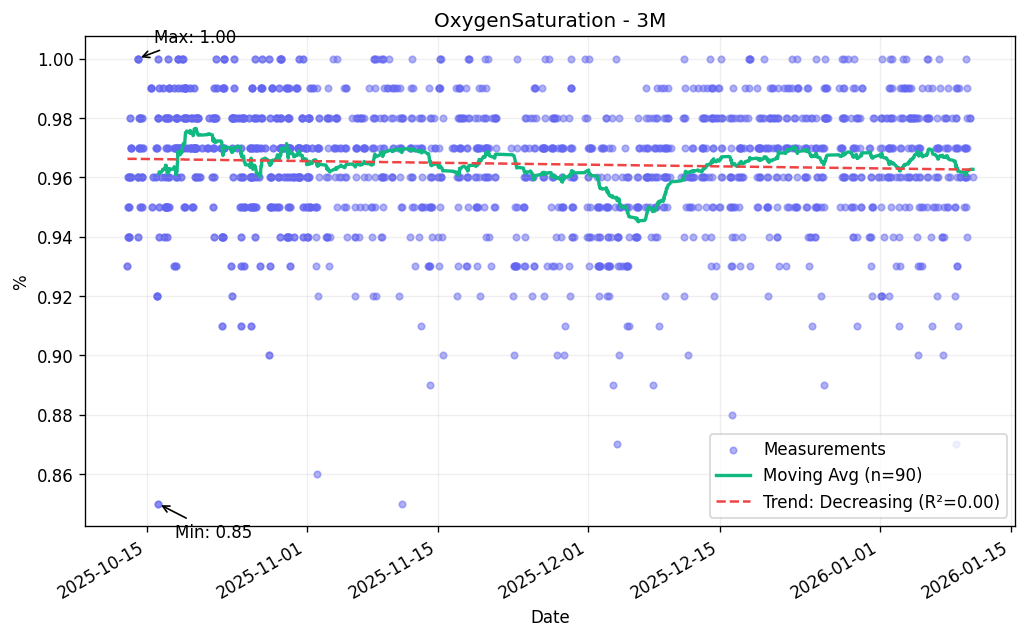
\includegraphics[width=0.95\textwidth]{plots_medical/Respiratory/oxygensaturation_3M.png}
\end{figure}
\begin{figure}[H]
\centering
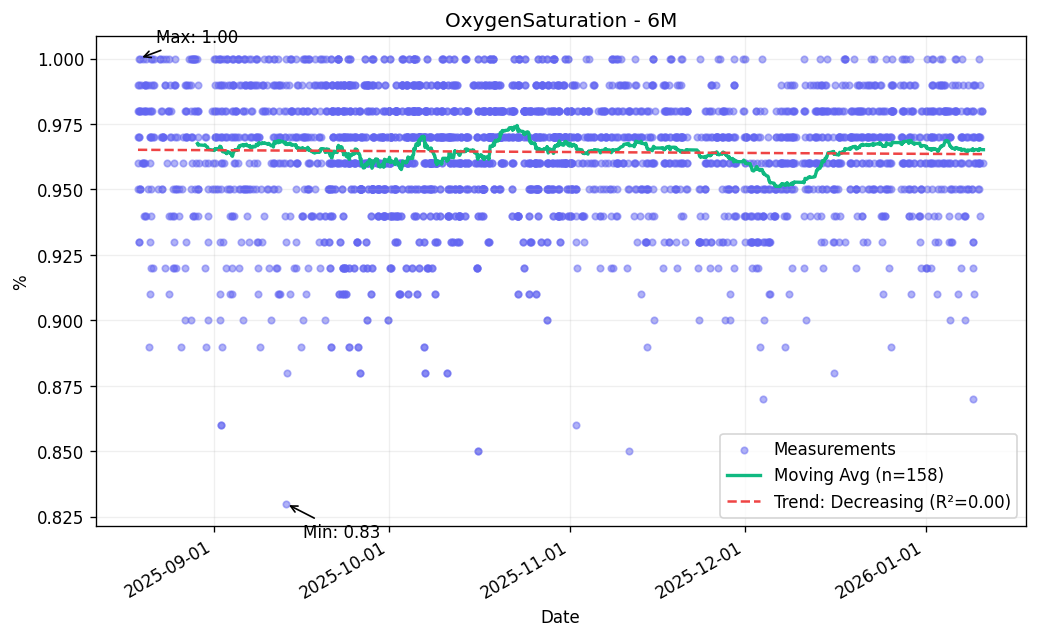
\includegraphics[width=0.95\textwidth]{plots_medical/Respiratory/oxygensaturation_6M.png}
\end{figure}
\begin{figure}[H]
\centering
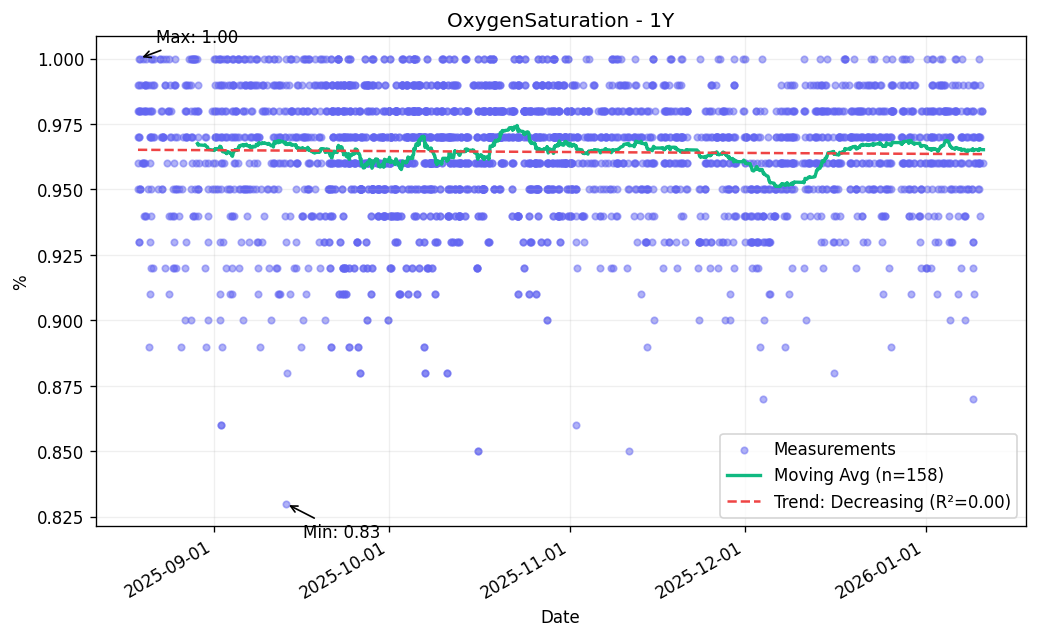
\includegraphics[width=0.95\textwidth]{plots_medical/Respiratory/oxygensaturation_1Y.png}
\end{figure}
\begin{figure}[H]
\centering
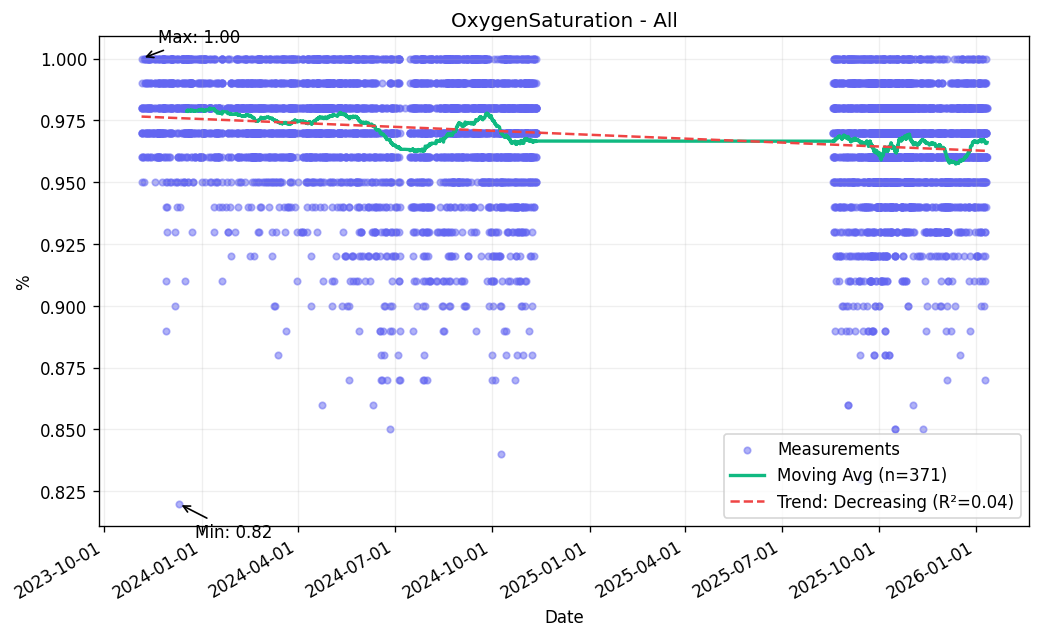
\includegraphics[width=0.95\textwidth]{plots_medical/Respiratory/oxygensaturation_All.png}
\end{figure}
\clearpage
\subsection{RespiratoryRate}
\begin{table}[H]
\centering
\resizebox{\textwidth}{!}{
\begin{tabular}{|l|c|c|c|c|c|c|}
\hline
\textbf{Window} & \textbf{Min} & \textbf{Max} & \textbf{Avg} & \textbf{Start} & \textbf{End} & \textbf{Trend Slope} \\ \hline
1W & 13.00 count/min & 35.50 count/min & 17.00 count/min & 19.00 & 14.50 & -0.25668 \\ \hline
1M & 8.50 count/min & 35.50 count/min & 16.90 count/min & 18.50 & 14.50 & -0.01726 \\ \hline
3M & 7.00 count/min & 35.50 count/min & 17.34 count/min & 22.50 & 14.50 & -0.00527 \\ \hline
6M & 7.00 count/min & 35.50 count/min & 17.11 count/min & 20.00 & 14.50 & 0.00460 \\ \hline
1Y & 7.00 count/min & 35.50 count/min & 16.62 count/min & 15.00 & 14.50 & 0.00553 \\ \hline
All & 7.00 count/min & 35.50 count/min & 16.27 count/min & 16.50 & 14.50 & 0.00279 \\ \hline
\end{tabular}
}
\caption{Detailed Statistics for RespiratoryRate}
\end{table}
\begin{figure}[H]
\centering
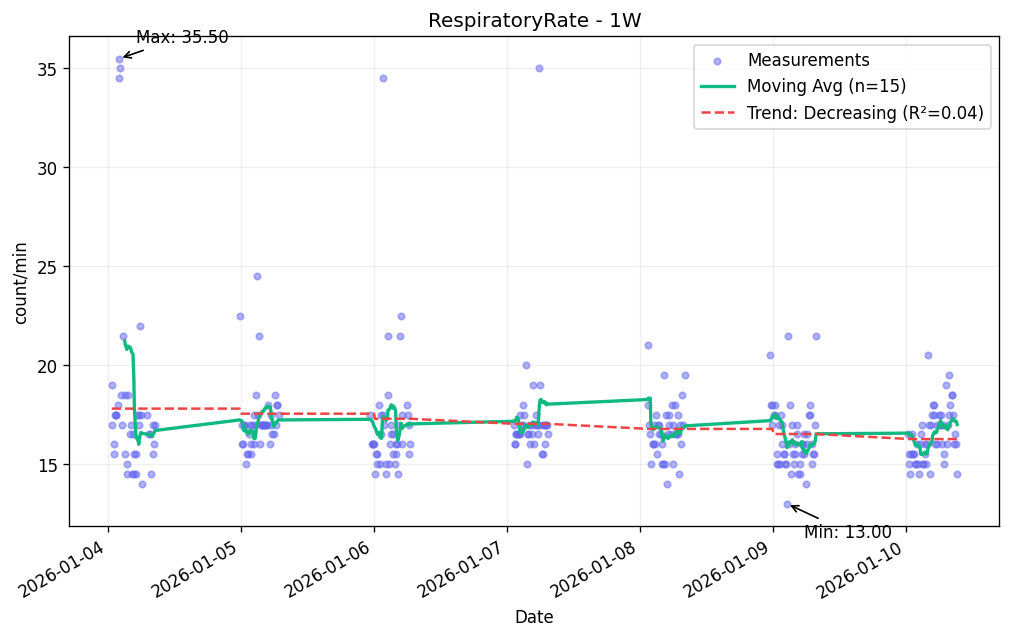
\includegraphics[width=0.95\textwidth]{plots_medical/Respiratory/respiratoryrate_1W.png}
\end{figure}
\begin{figure}[H]
\centering
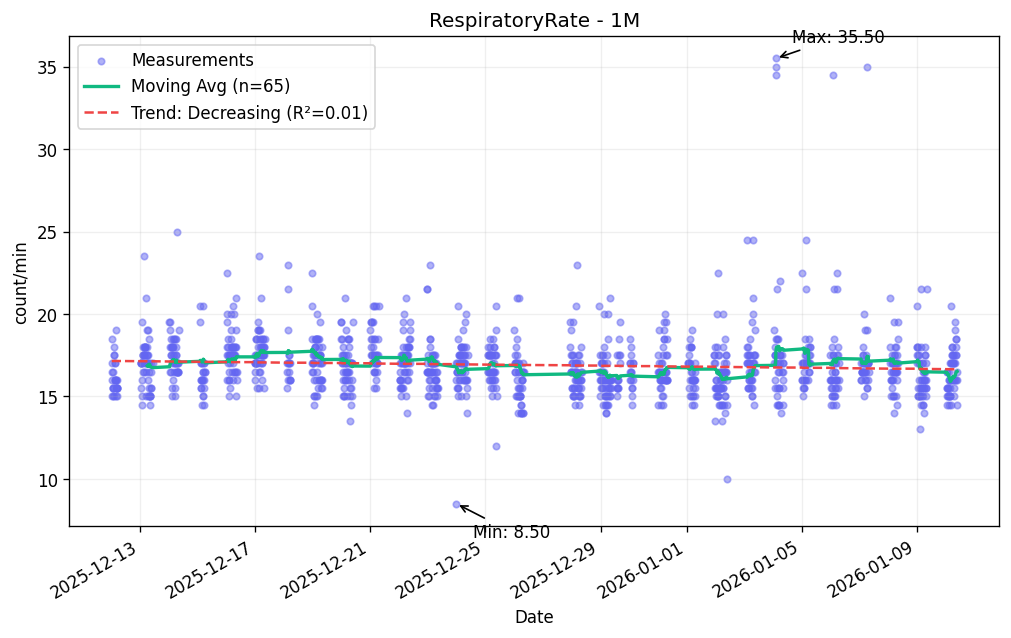
\includegraphics[width=0.95\textwidth]{plots_medical/Respiratory/respiratoryrate_1M.png}
\end{figure}
\begin{figure}[H]
\centering
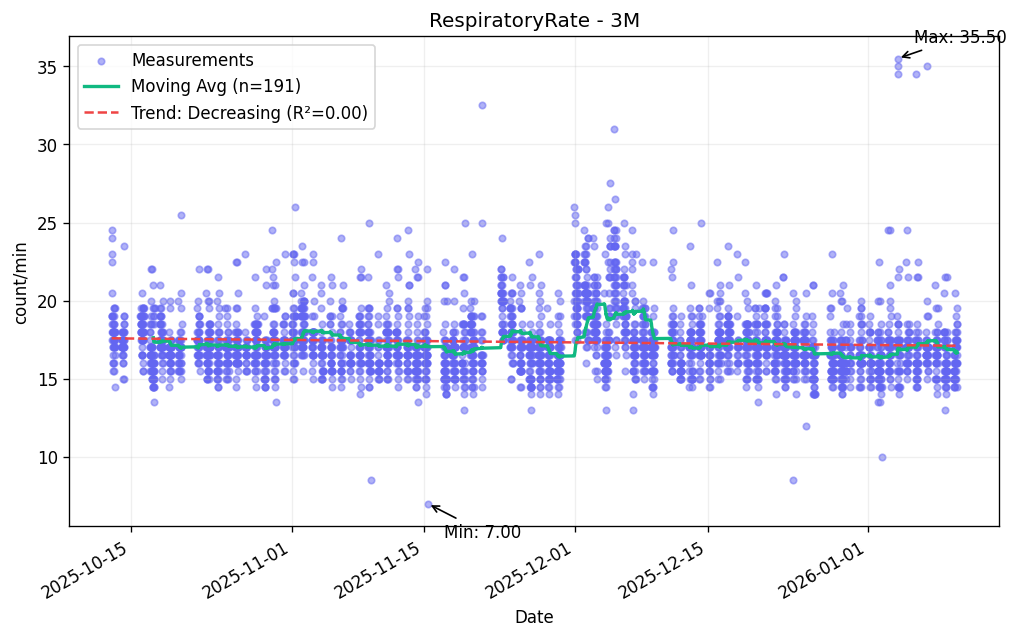
\includegraphics[width=0.95\textwidth]{plots_medical/Respiratory/respiratoryrate_3M.png}
\end{figure}
\begin{figure}[H]
\centering
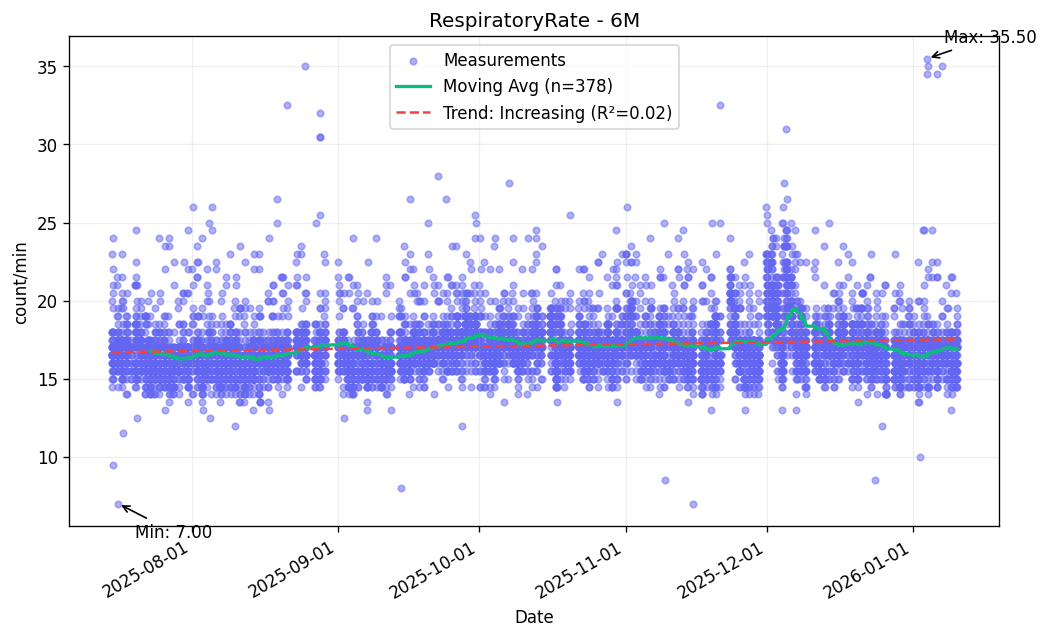
\includegraphics[width=0.95\textwidth]{plots_medical/Respiratory/respiratoryrate_6M.png}
\end{figure}
\begin{figure}[H]
\centering
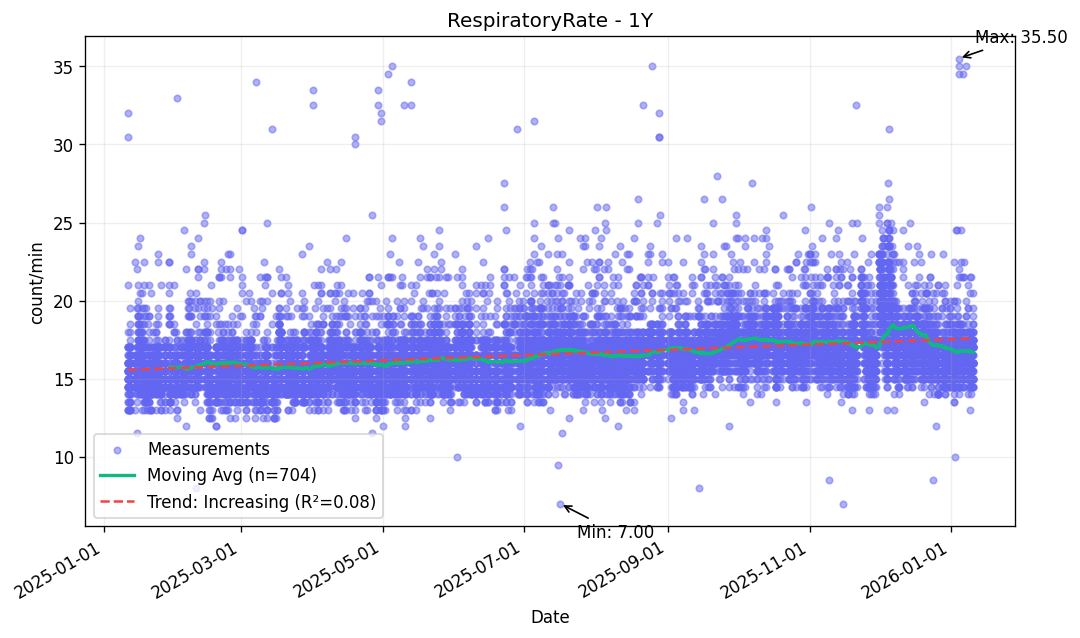
\includegraphics[width=0.95\textwidth]{plots_medical/Respiratory/respiratoryrate_1Y.png}
\end{figure}
\begin{figure}[H]
\centering
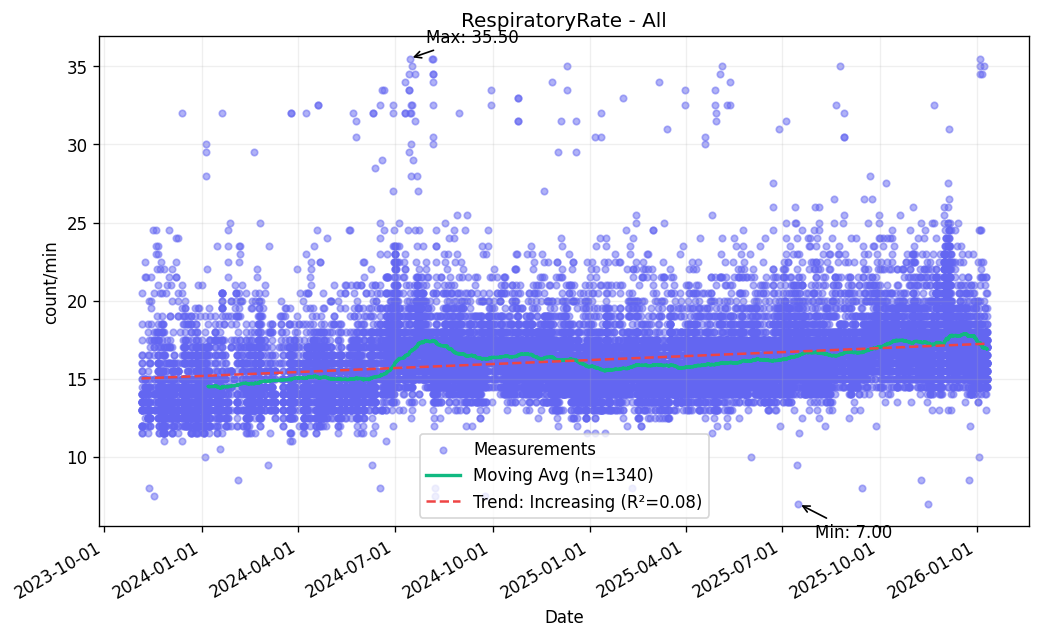
\includegraphics[width=0.95\textwidth]{plots_medical/Respiratory/respiratoryrate_All.png}
\end{figure}
\clearpage
\section{Vitals \& Body Measurements}
\subsection{BodyFatPercentage}
\begin{table}[H]
\centering
\resizebox{\textwidth}{!}{
\begin{tabular}{|l|c|c|c|c|c|c|}
\hline
\textbf{Window} & \textbf{Min} & \textbf{Max} & \textbf{Avg} & \textbf{Start} & \textbf{End} & \textbf{Trend Slope} \\ \hline
1W & - & - & - & - & - & - \\ \hline
1M & - & - & - & - & - & - \\ \hline
3M & 0.22 \% & 0.23 \% & 0.22 \% & 0.22 & 0.23 & 0.00006 \\ \hline
6M & 0.22 \% & 0.26 \% & 0.24 \% & 0.26 & 0.23 & -0.00029 \\ \hline
1Y & 0.22 \% & 0.26 \% & 0.24 \% & 0.26 & 0.23 & -0.00029 \\ \hline
All & 0.22 \% & 0.26 \% & 0.24 \% & 0.22 & 0.23 & 0.00005 \\ \hline
\end{tabular}
}
\caption{Detailed Statistics for BodyFatPercentage}
\end{table}
\begin{figure}[H]
\centering
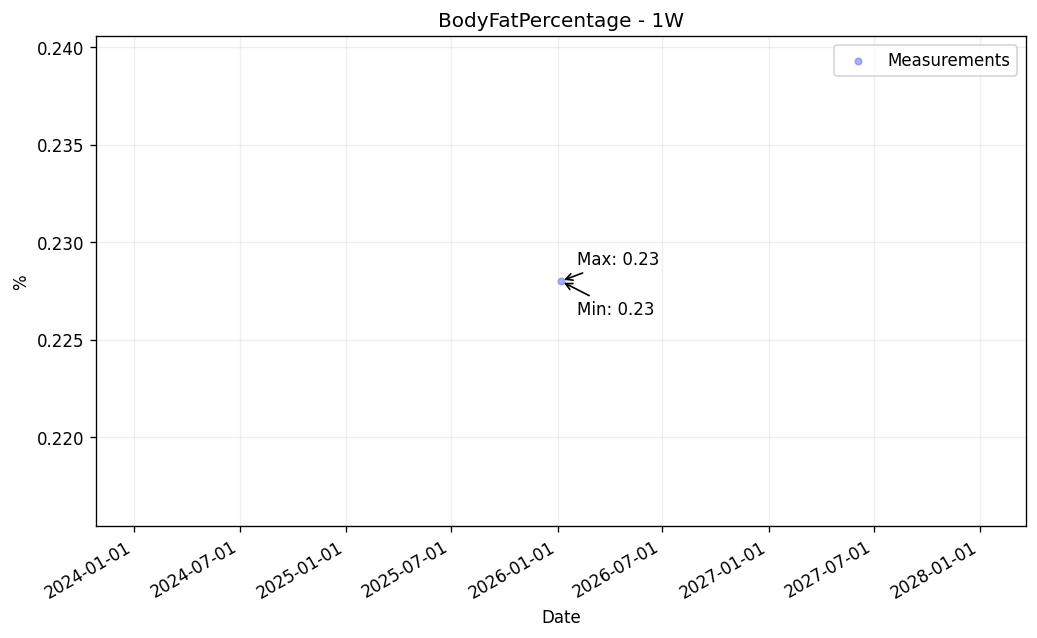
\includegraphics[width=0.95\textwidth]{plots_medical/Vitals_and_Body_Measurements/bodyfatpercentage_1W.png}
\end{figure}
\begin{figure}[H]
\centering
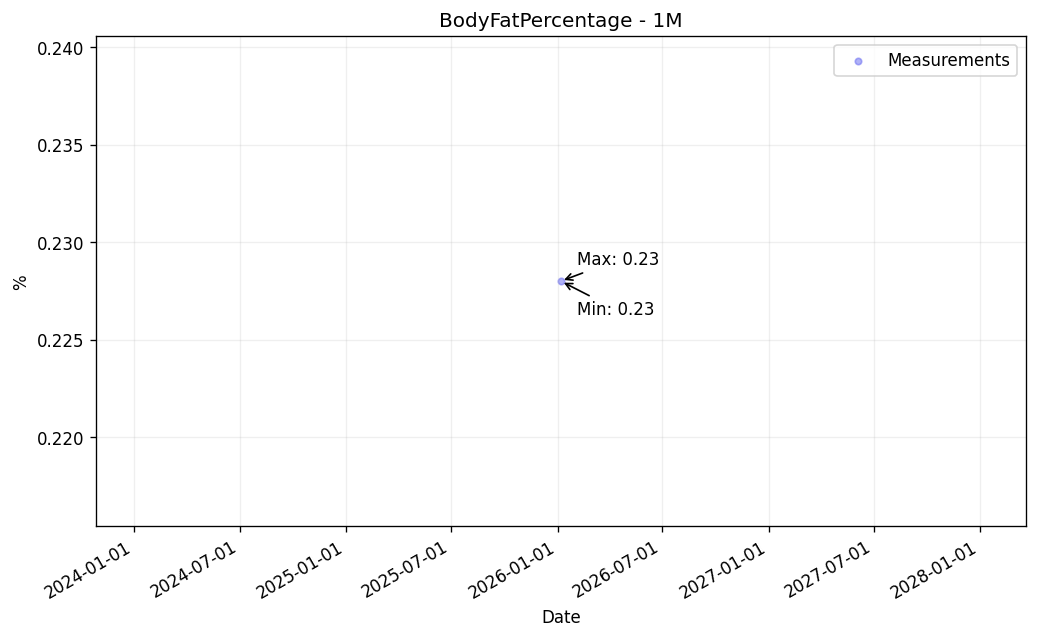
\includegraphics[width=0.95\textwidth]{plots_medical/Vitals_and_Body_Measurements/bodyfatpercentage_1M.png}
\end{figure}
\begin{figure}[H]
\centering
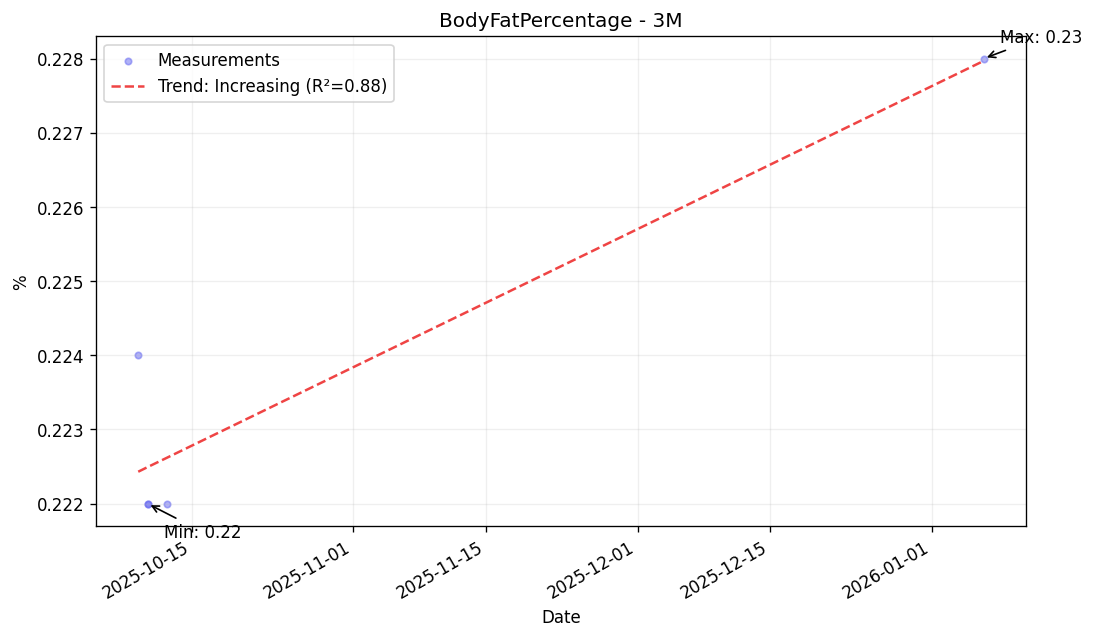
\includegraphics[width=0.95\textwidth]{plots_medical/Vitals_and_Body_Measurements/bodyfatpercentage_3M.png}
\end{figure}
\begin{figure}[H]
\centering
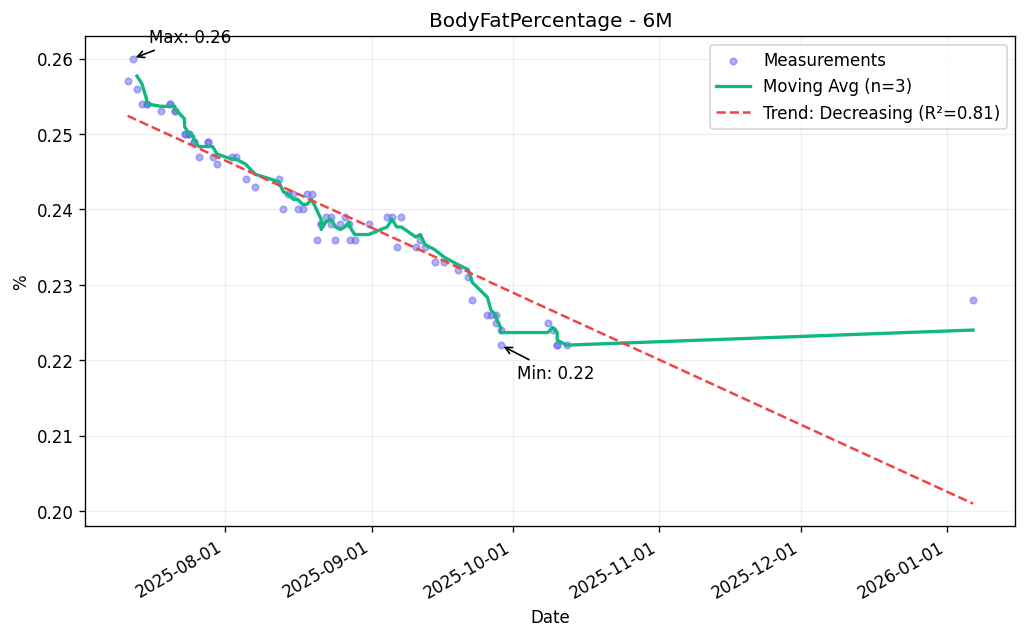
\includegraphics[width=0.95\textwidth]{plots_medical/Vitals_and_Body_Measurements/bodyfatpercentage_6M.png}
\end{figure}
\begin{figure}[H]
\centering
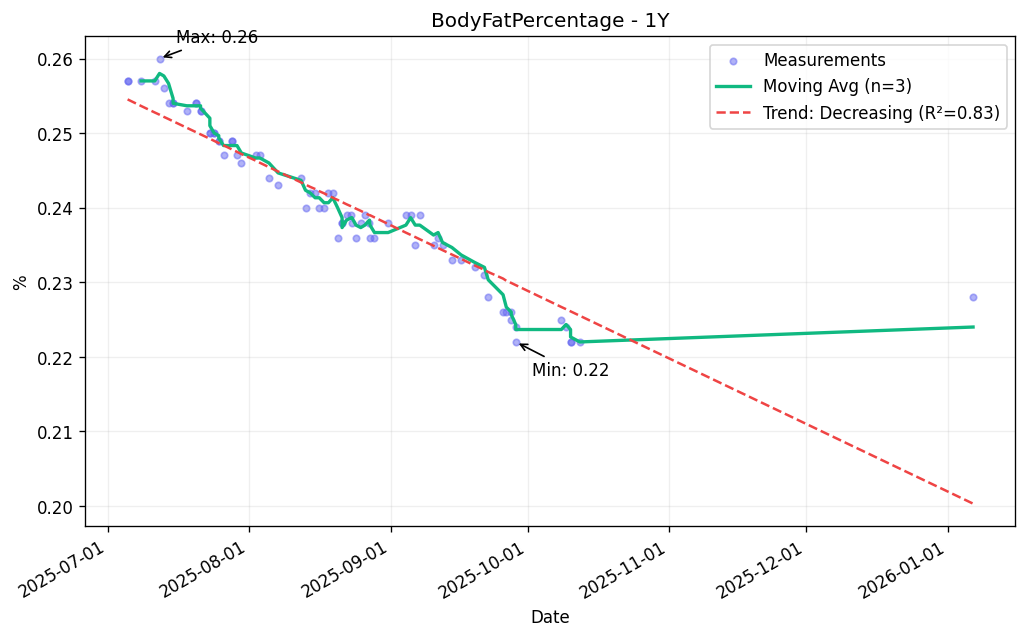
\includegraphics[width=0.95\textwidth]{plots_medical/Vitals_and_Body_Measurements/bodyfatpercentage_1Y.png}
\end{figure}
\begin{figure}[H]
\centering
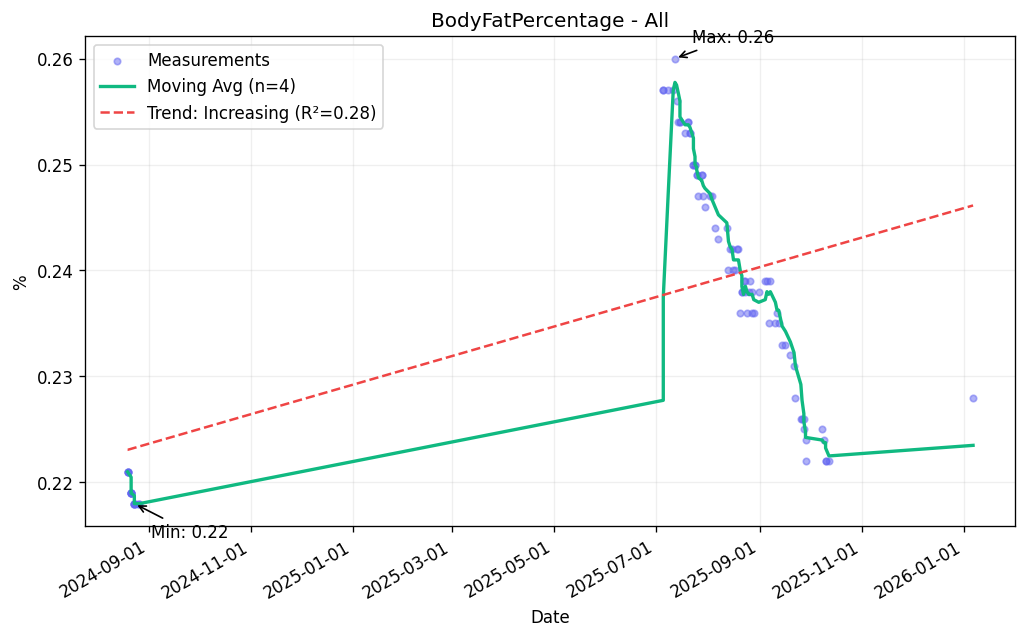
\includegraphics[width=0.95\textwidth]{plots_medical/Vitals_and_Body_Measurements/bodyfatpercentage_All.png}
\end{figure}
\clearpage
\subsection{BodyMass}
\begin{table}[H]
\centering
\resizebox{\textwidth}{!}{
\begin{tabular}{|l|c|c|c|c|c|c|}
\hline
\textbf{Window} & \textbf{Min} & \textbf{Max} & \textbf{Avg} & \textbf{Start} & \textbf{End} & \textbf{Trend Slope} \\ \hline
1W & 195.80 lb & 198.20 lb & 197.00 lb & 198.20 & 195.80 & -0.48000 \\ \hline
1M & 195.80 lb & 198.20 lb & 197.00 lb & 198.20 & 195.80 & -0.48000 \\ \hline
3M & 192.80 lb & 198.20 lb & 194.31 lb & 194.20 & 195.80 & 0.03942 \\ \hline
6M & 192.80 lb & 211.60 lb & 201.92 lb & 210.00 & 195.80 & -0.14734 \\ \hline
1Y & 192.80 lb & 216.00 lb & 202.68 lb & 205.20 & 195.80 & -0.08612 \\ \hline
All & 143.00 lb & 216.00 lb & 194.28 lb & 143.00 & 195.80 & 0.02279 \\ \hline
\end{tabular}
}
\caption{Detailed Statistics for BodyMass}
\end{table}
\begin{figure}[H]
\centering
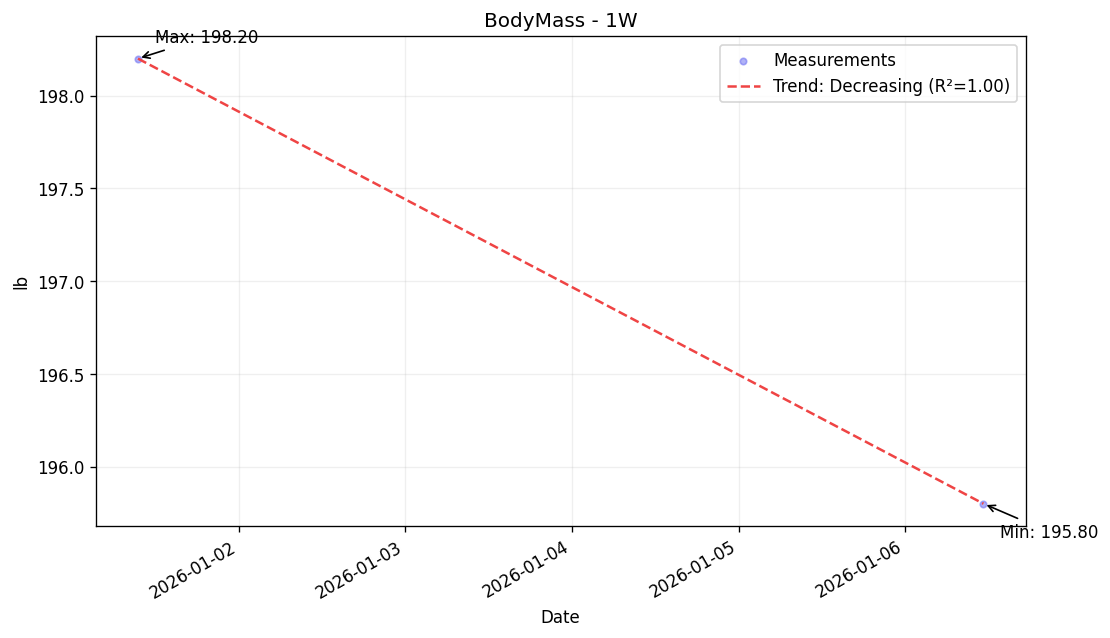
\includegraphics[width=0.95\textwidth]{plots_medical/Vitals_and_Body_Measurements/bodymass_1W.png}
\end{figure}
\begin{figure}[H]
\centering
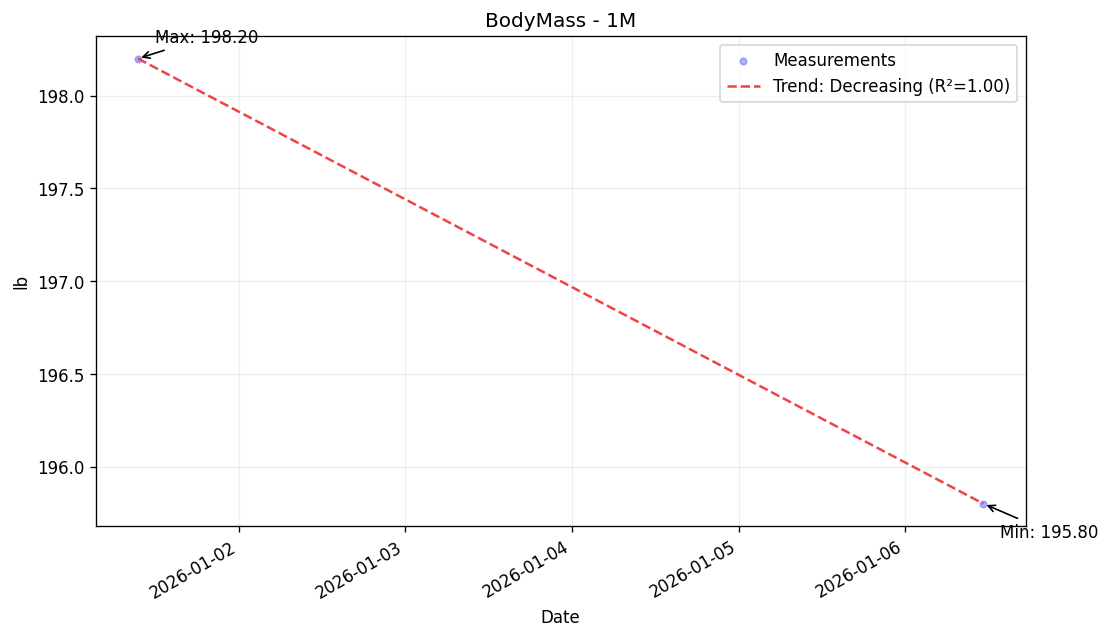
\includegraphics[width=0.95\textwidth]{plots_medical/Vitals_and_Body_Measurements/bodymass_1M.png}
\end{figure}
\begin{figure}[H]
\centering
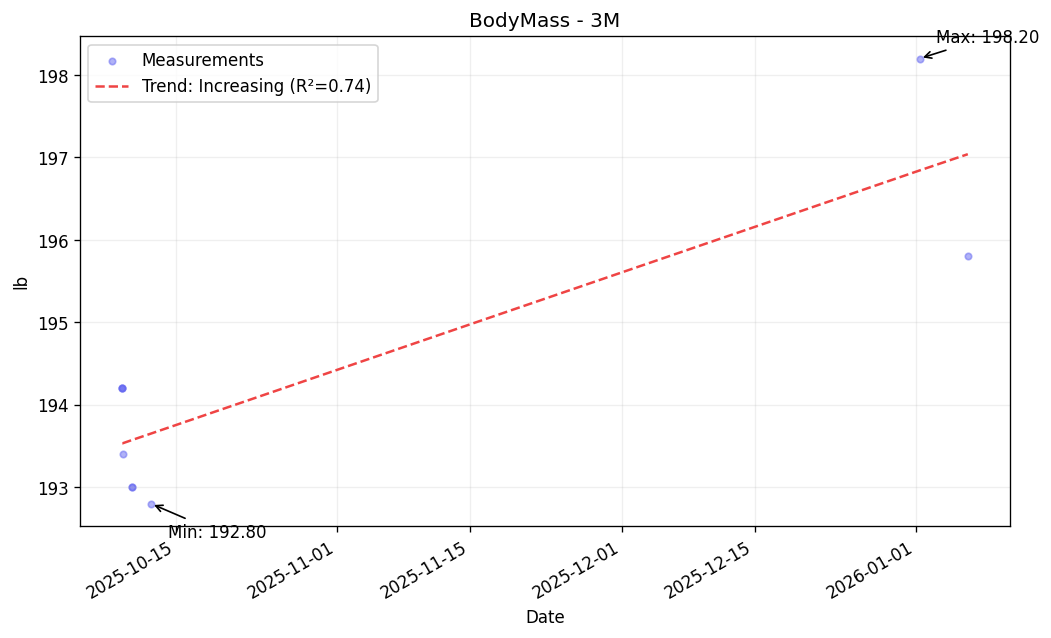
\includegraphics[width=0.95\textwidth]{plots_medical/Vitals_and_Body_Measurements/bodymass_3M.png}
\end{figure}
\begin{figure}[H]
\centering
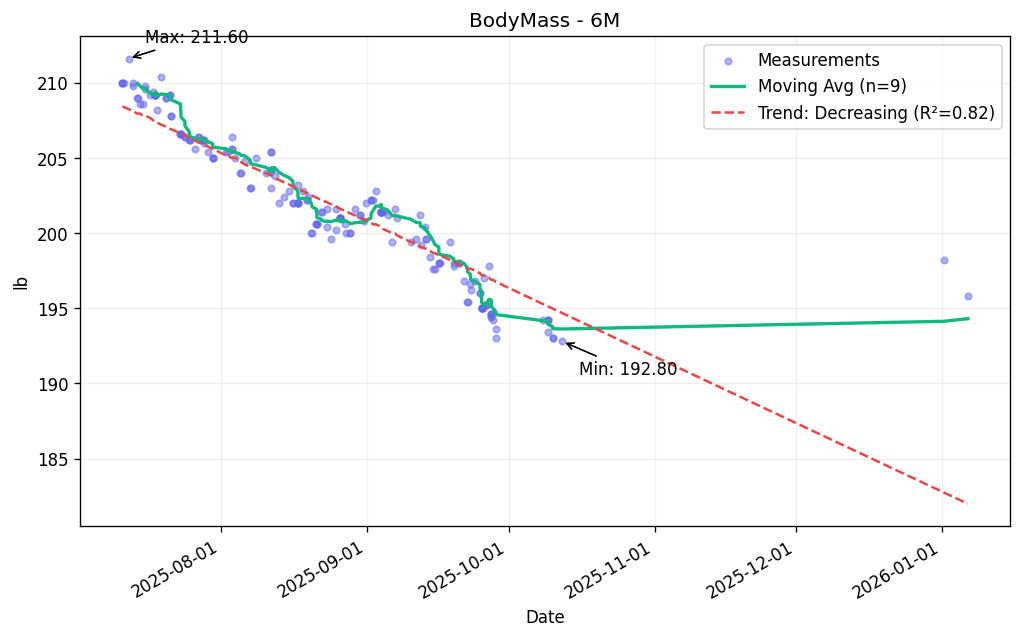
\includegraphics[width=0.95\textwidth]{plots_medical/Vitals_and_Body_Measurements/bodymass_6M.png}
\end{figure}
\begin{figure}[H]
\centering
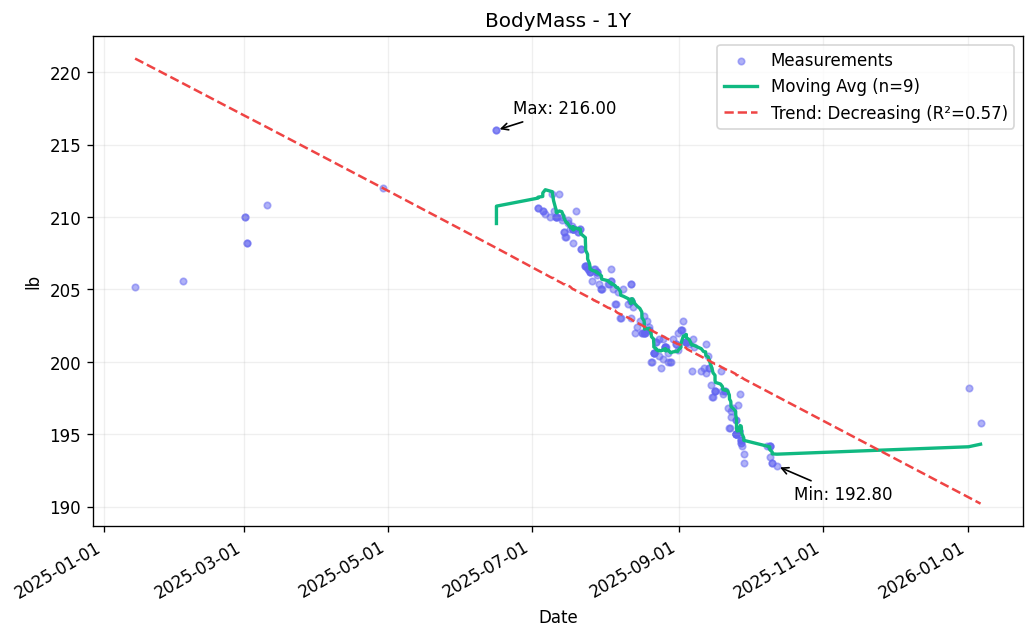
\includegraphics[width=0.95\textwidth]{plots_medical/Vitals_and_Body_Measurements/bodymass_1Y.png}
\end{figure}
\begin{figure}[H]
\centering
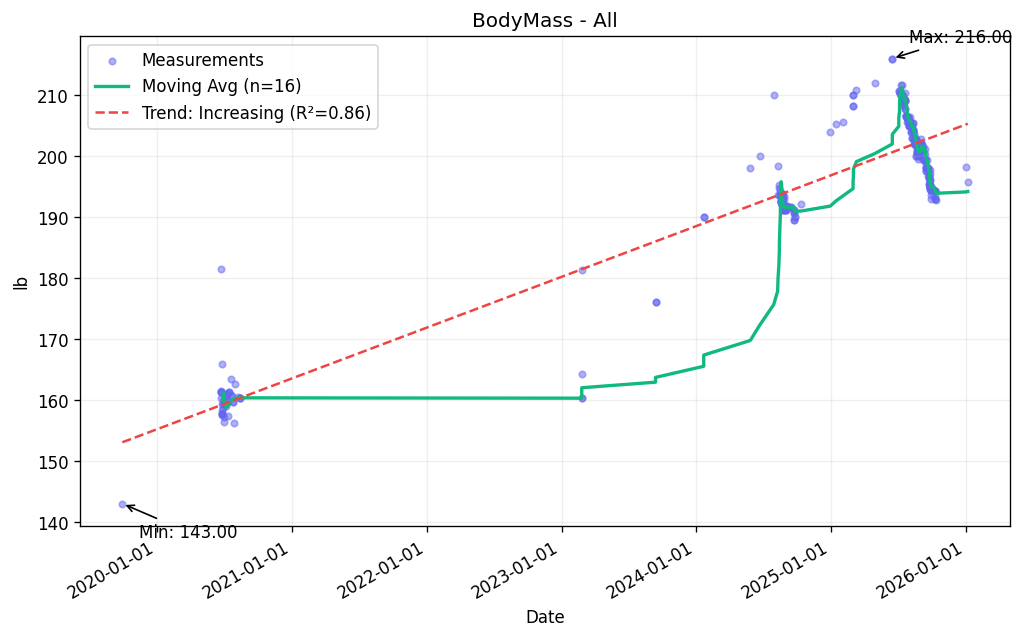
\includegraphics[width=0.95\textwidth]{plots_medical/Vitals_and_Body_Measurements/bodymass_All.png}
\end{figure}
\clearpage
\subsection{BodyMassIndex}
\begin{table}[H]
\centering
\resizebox{\textwidth}{!}{
\begin{tabular}{|l|c|c|c|c|c|c|}
\hline
\textbf{Window} & \textbf{Min} & \textbf{Max} & \textbf{Avg} & \textbf{Start} & \textbf{End} & \textbf{Trend Slope} \\ \hline
1W & - & - & - & - & - & - \\ \hline
1M & - & - & - & - & - & - \\ \hline
3M & 27.60 count & 28.00 count & 27.74 count & 27.80 & 28.00 & 0.00332 \\ \hline
6M & 27.60 count & 30.30 count & 28.93 count & 30.10 & 28.00 & -0.02314 \\ \hline
1Y & 27.60 count & 30.99 count & 29.01 count & 29.44 & 28.00 & -0.01387 \\ \hline
All & 22.36 count & 30.99 count & 27.91 count & 22.90 & 28.00 & 0.00319 \\ \hline
\end{tabular}
}
\caption{Detailed Statistics for BodyMassIndex}
\end{table}
\begin{figure}[H]
\centering
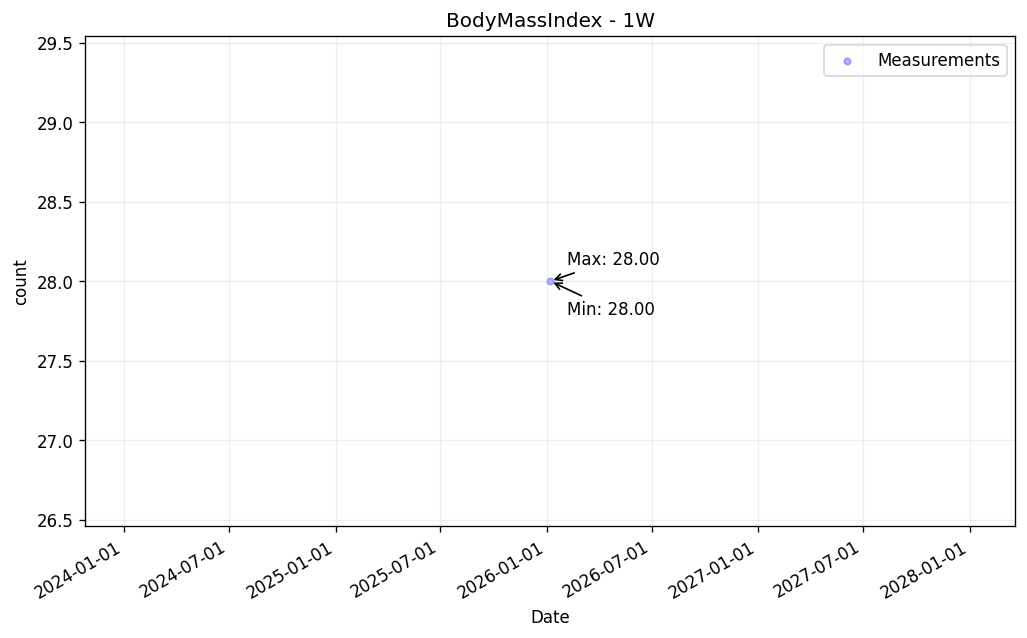
\includegraphics[width=0.95\textwidth]{plots_medical/Vitals_and_Body_Measurements/bodymassindex_1W.png}
\end{figure}
\begin{figure}[H]
\centering
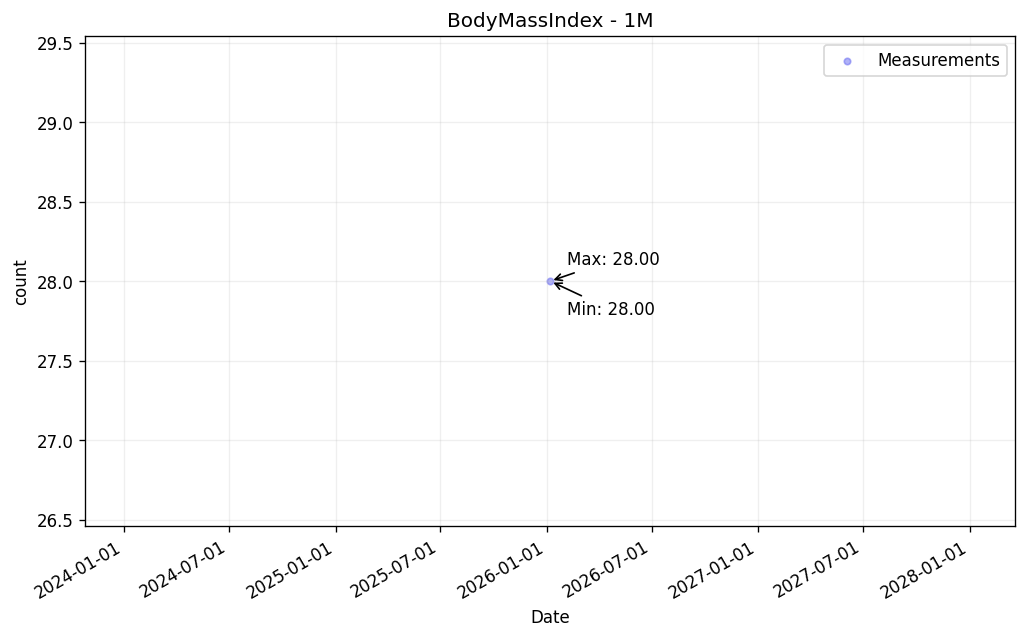
\includegraphics[width=0.95\textwidth]{plots_medical/Vitals_and_Body_Measurements/bodymassindex_1M.png}
\end{figure}
\begin{figure}[H]
\centering
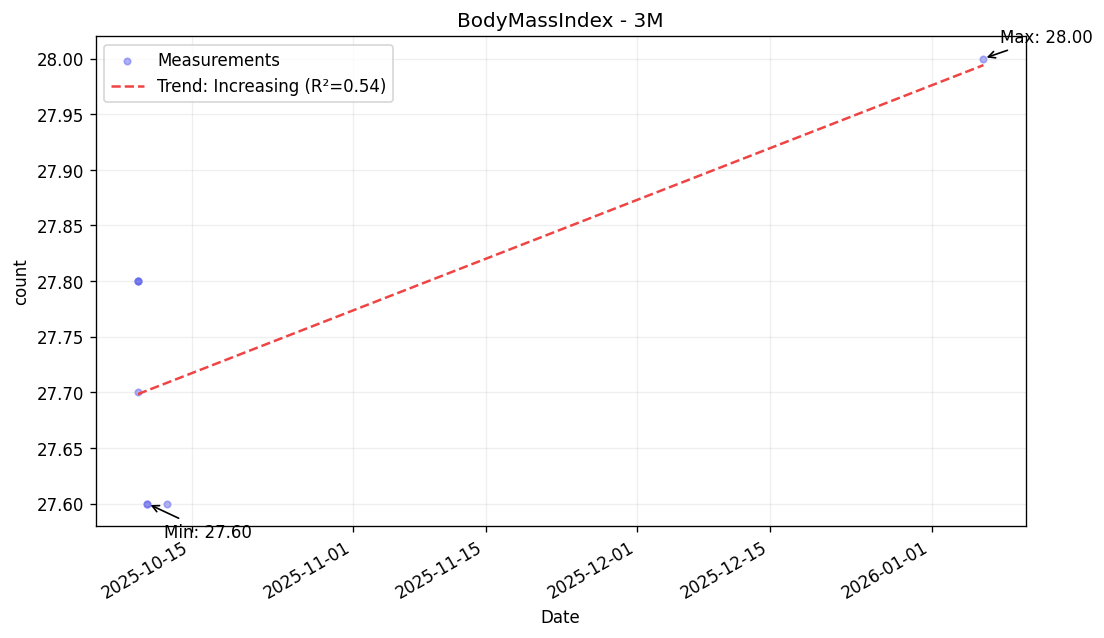
\includegraphics[width=0.95\textwidth]{plots_medical/Vitals_and_Body_Measurements/bodymassindex_3M.png}
\end{figure}
\begin{figure}[H]
\centering
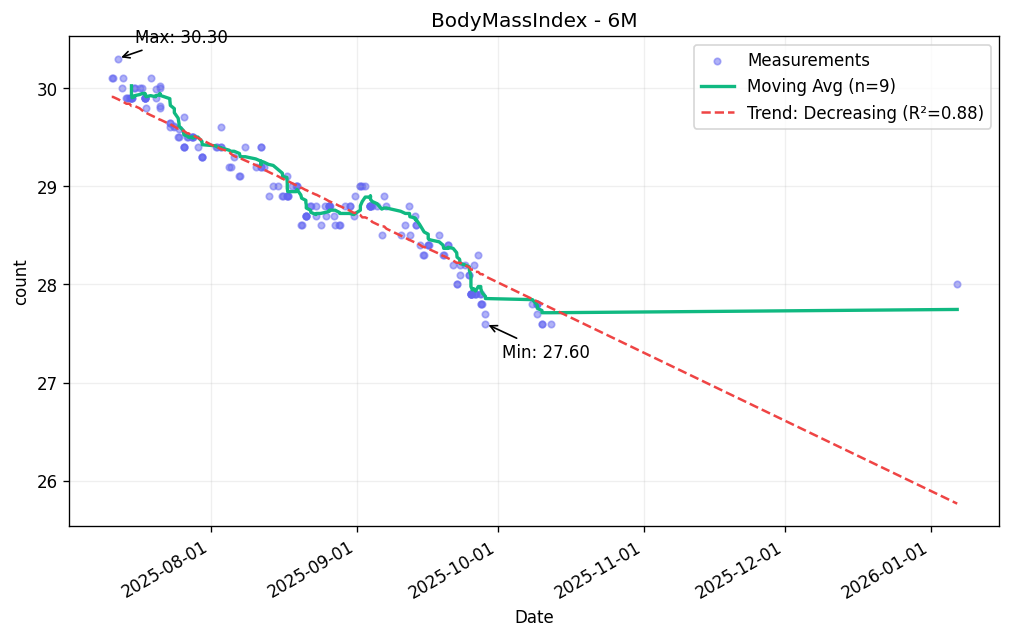
\includegraphics[width=0.95\textwidth]{plots_medical/Vitals_and_Body_Measurements/bodymassindex_6M.png}
\end{figure}
\begin{figure}[H]
\centering
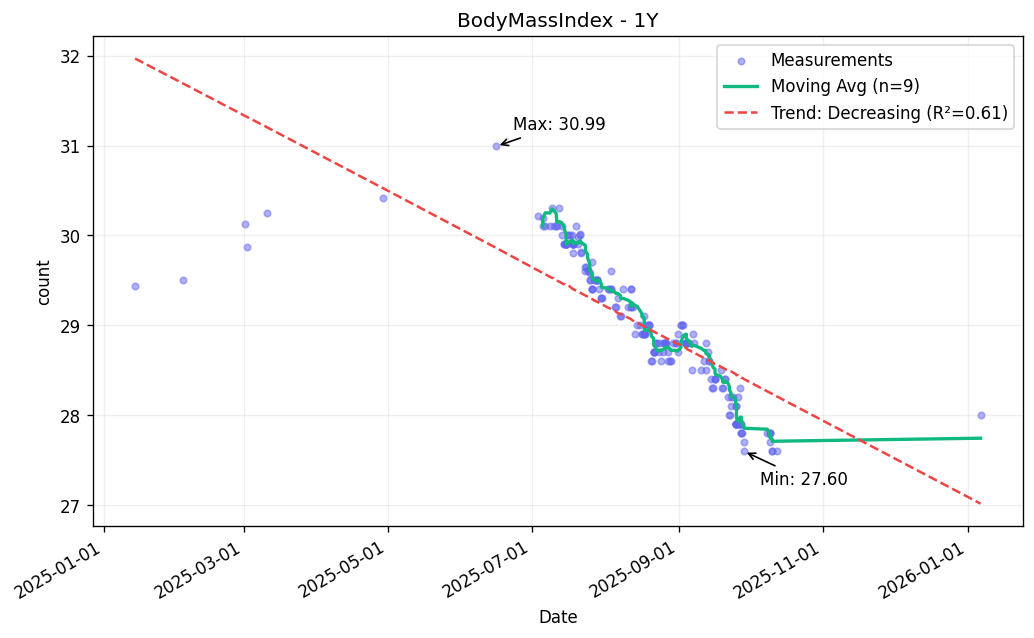
\includegraphics[width=0.95\textwidth]{plots_medical/Vitals_and_Body_Measurements/bodymassindex_1Y.png}
\end{figure}
\begin{figure}[H]
\centering
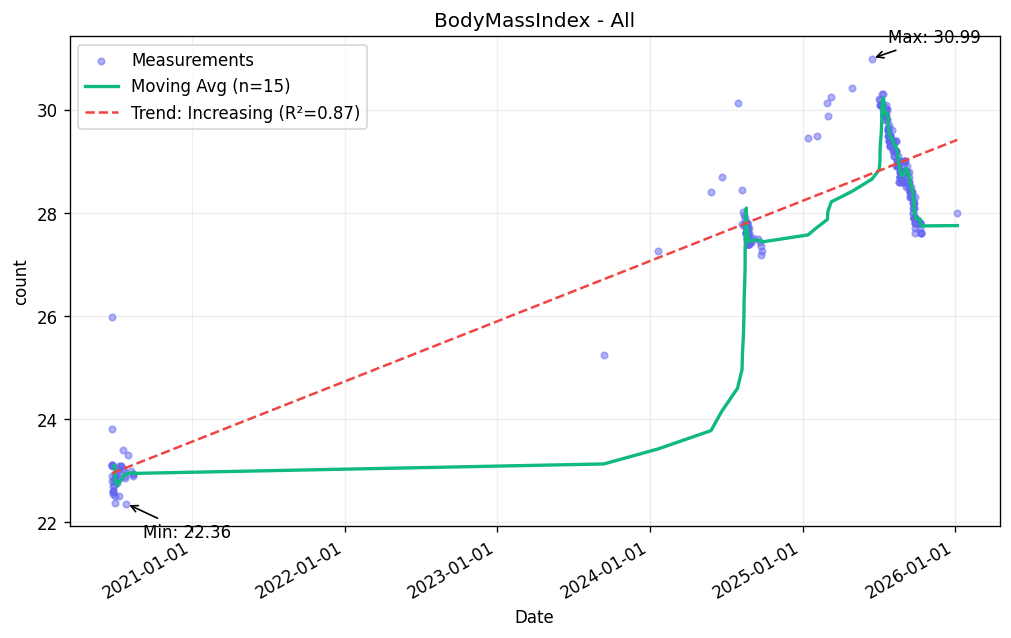
\includegraphics[width=0.95\textwidth]{plots_medical/Vitals_and_Body_Measurements/bodymassindex_All.png}
\end{figure}
\clearpage
\subsection{Height}
\begin{table}[H]
\centering
\resizebox{\textwidth}{!}{
\begin{tabular}{|l|c|c|c|c|c|c|}
\hline
\textbf{Window} & \textbf{Min} & \textbf{Max} & \textbf{Avg} & \textbf{Start} & \textbf{End} & \textbf{Trend Slope} \\ \hline
1W & - & - & - & - & - & - \\ \hline
1M & - & - & - & - & - & - \\ \hline
3M & 5.85 ft & 5.85 ft & 5.85 ft & 5.85 & 5.85 & 0.00000 \\ \hline
6M & 5.85 ft & 5.85 ft & 5.85 ft & 5.85 & 5.85 & 0.00000 \\ \hline
1Y & 5.85 ft & 5.85 ft & 5.85 ft & 5.85 & 5.85 & 0.00000 \\ \hline
All & 5.83 ft & 5.85 ft & 5.84 ft & 5.83 & 5.85 & 0.00001 \\ \hline
\end{tabular}
}
\caption{Detailed Statistics for Height}
\end{table}
\begin{figure}[H]
\centering
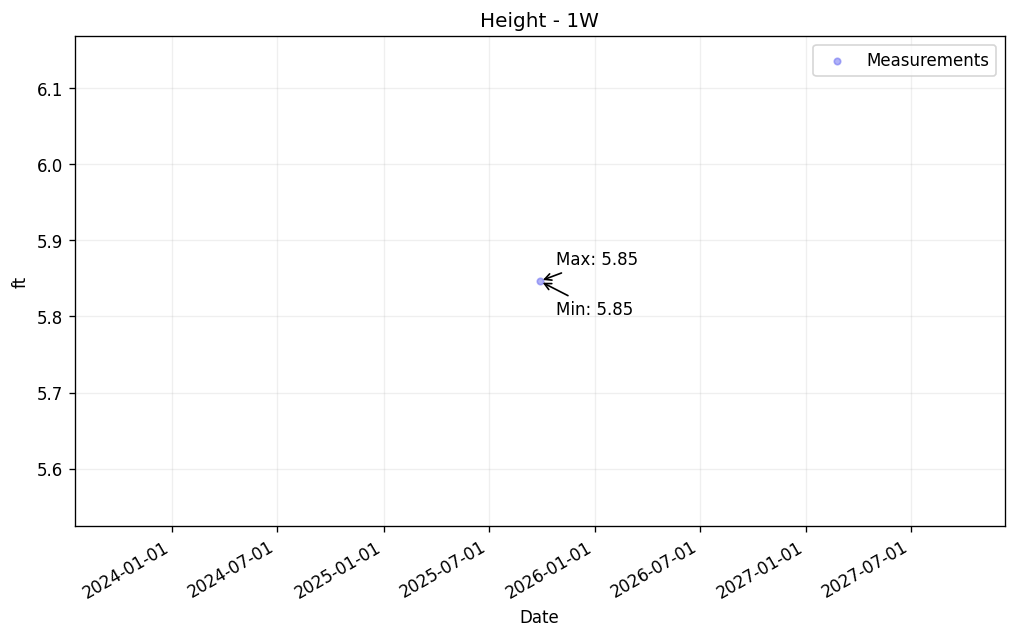
\includegraphics[width=0.95\textwidth]{plots_medical/Vitals_and_Body_Measurements/height_1W.png}
\end{figure}
\begin{figure}[H]
\centering
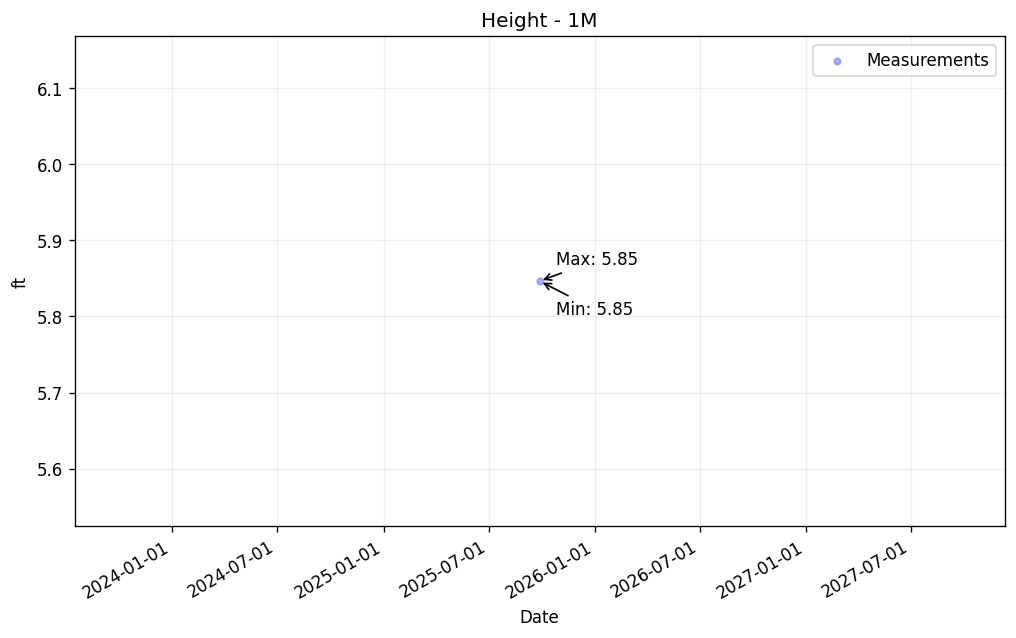
\includegraphics[width=0.95\textwidth]{plots_medical/Vitals_and_Body_Measurements/height_1M.png}
\end{figure}
\begin{figure}[H]
\centering
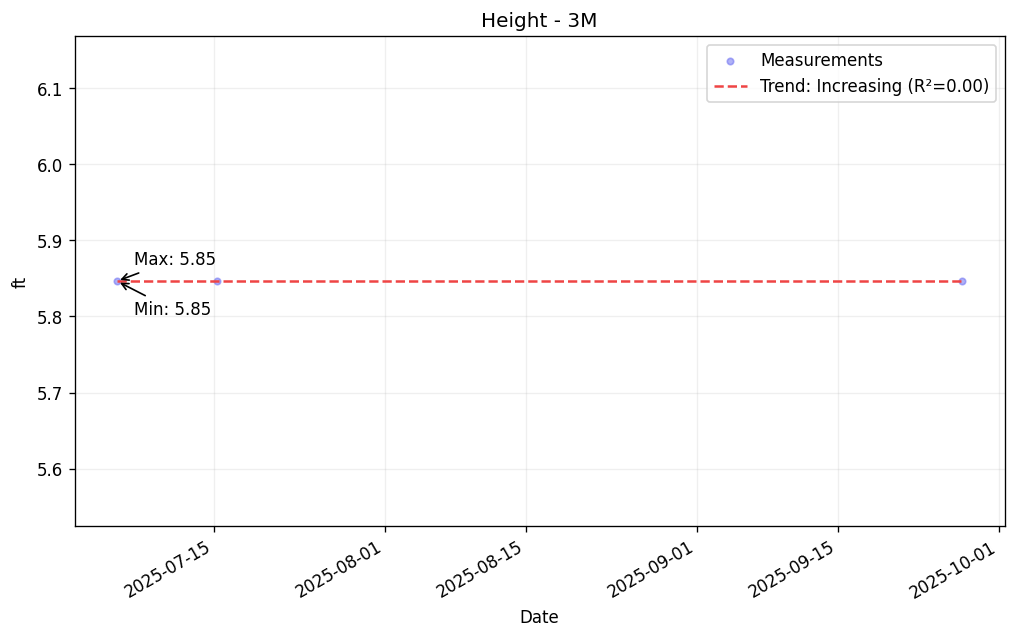
\includegraphics[width=0.95\textwidth]{plots_medical/Vitals_and_Body_Measurements/height_3M.png}
\end{figure}
\begin{figure}[H]
\centering
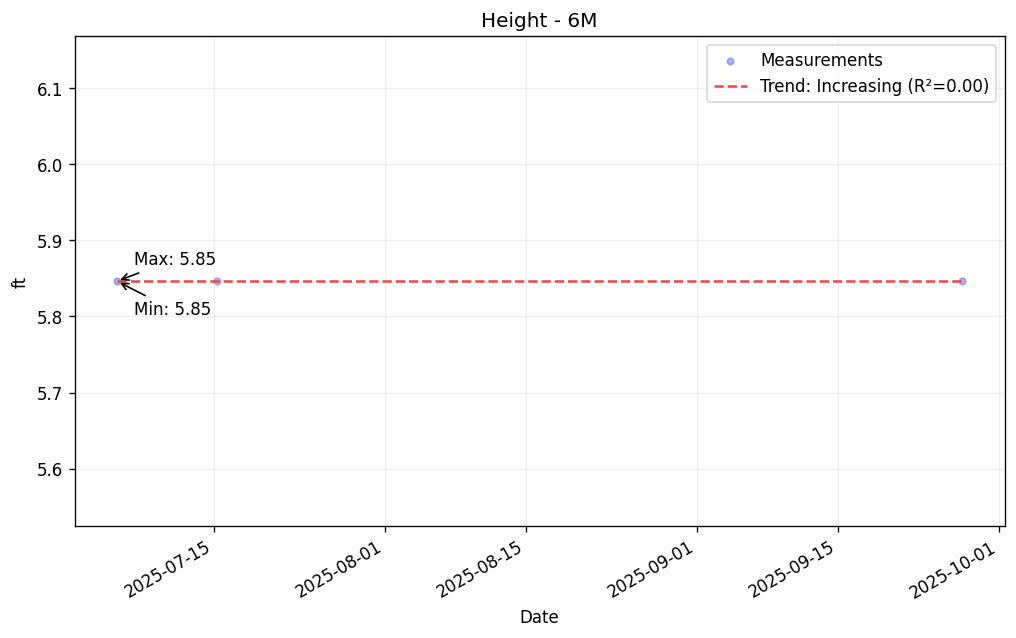
\includegraphics[width=0.95\textwidth]{plots_medical/Vitals_and_Body_Measurements/height_6M.png}
\end{figure}
\begin{figure}[H]
\centering
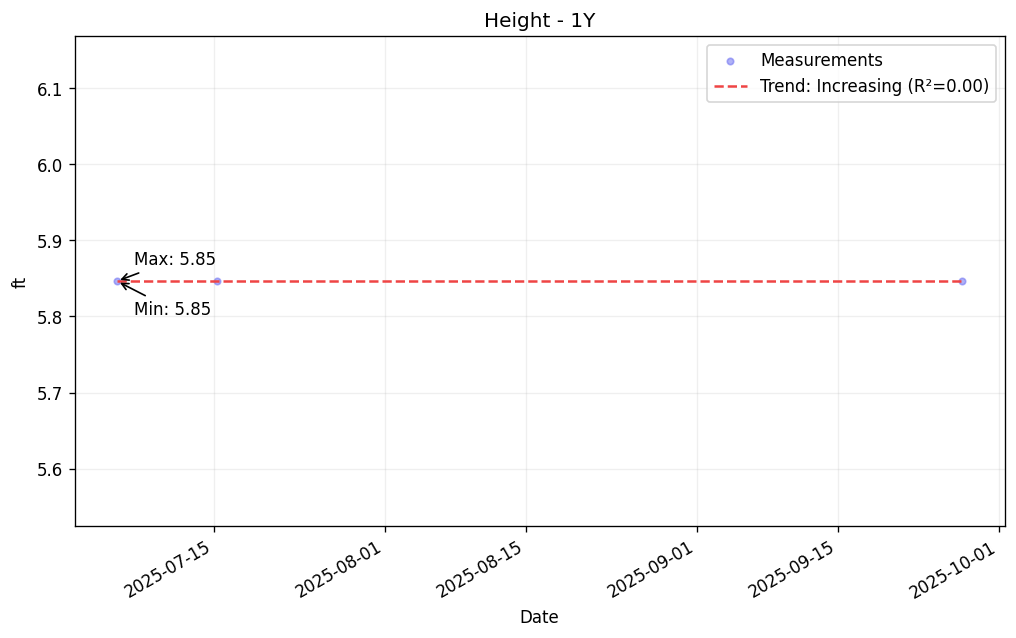
\includegraphics[width=0.95\textwidth]{plots_medical/Vitals_and_Body_Measurements/height_1Y.png}
\end{figure}
\begin{figure}[H]
\centering
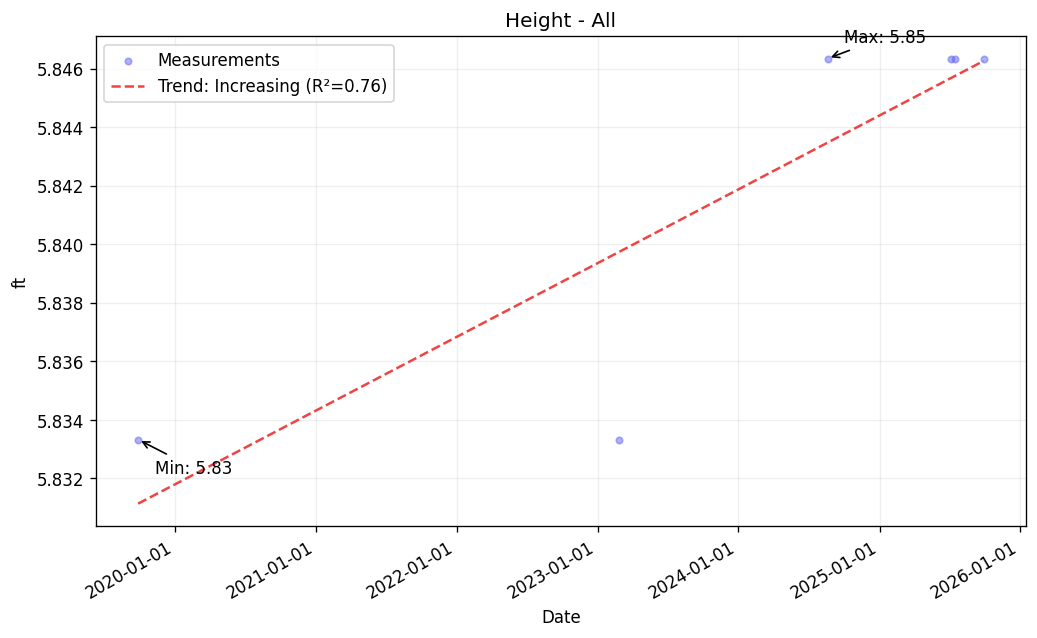
\includegraphics[width=0.95\textwidth]{plots_medical/Vitals_and_Body_Measurements/height_All.png}
\end{figure}
\clearpage
\subsection{LeanBodyMass}
\begin{table}[H]
\centering
\resizebox{\textwidth}{!}{
\begin{tabular}{|l|c|c|c|c|c|c|}
\hline
\textbf{Window} & \textbf{Min} & \textbf{Max} & \textbf{Avg} & \textbf{Start} & \textbf{End} & \textbf{Trend Slope} \\ \hline
1W & - & - & - & - & - & - \\ \hline
1M & - & - & - & - & - & - \\ \hline
3M & 150.00 lb & 151.20 lb & 150.36 lb & 150.20 & 151.20 & 0.01190 \\ \hline
6M & 150.00 lb & 156.80 lb & 153.15 lb & 156.00 & 151.20 & -0.04960 \\ \hline
1Y & 150.00 lb & 156.80 lb & 153.24 lb & 156.40 & 151.20 & -0.05043 \\ \hline
All & 149.40 lb & 156.80 lb & 152.82 lb & 150.00 & 151.20 & 0.00577 \\ \hline
\end{tabular}
}
\caption{Detailed Statistics for LeanBodyMass}
\end{table}
\begin{figure}[H]
\centering
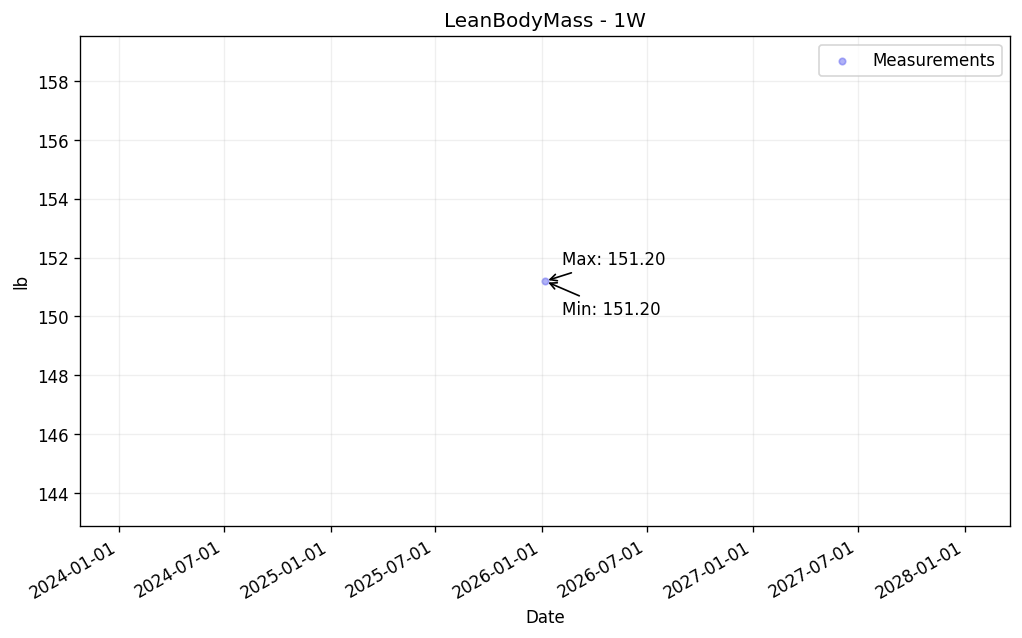
\includegraphics[width=0.95\textwidth]{plots_medical/Vitals_and_Body_Measurements/leanbodymass_1W.png}
\end{figure}
\begin{figure}[H]
\centering
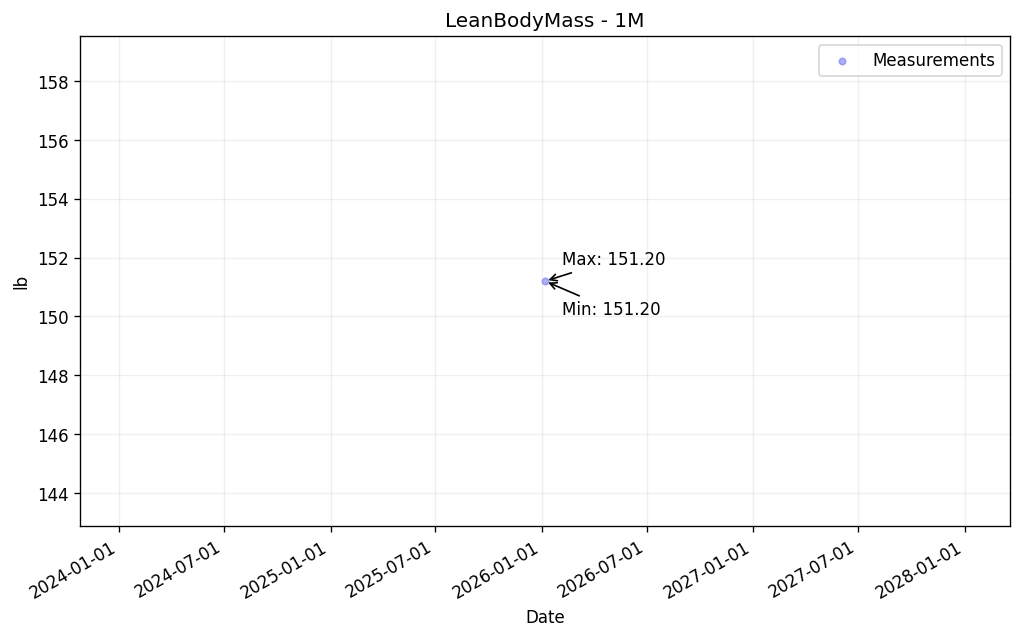
\includegraphics[width=0.95\textwidth]{plots_medical/Vitals_and_Body_Measurements/leanbodymass_1M.png}
\end{figure}
\begin{figure}[H]
\centering
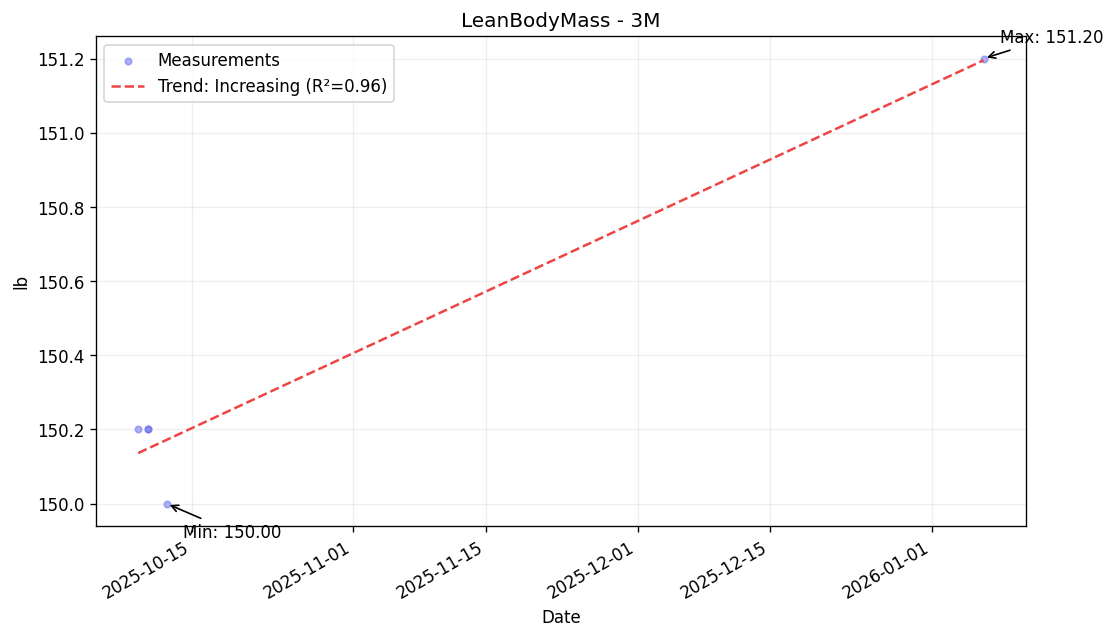
\includegraphics[width=0.95\textwidth]{plots_medical/Vitals_and_Body_Measurements/leanbodymass_3M.png}
\end{figure}
\begin{figure}[H]
\centering
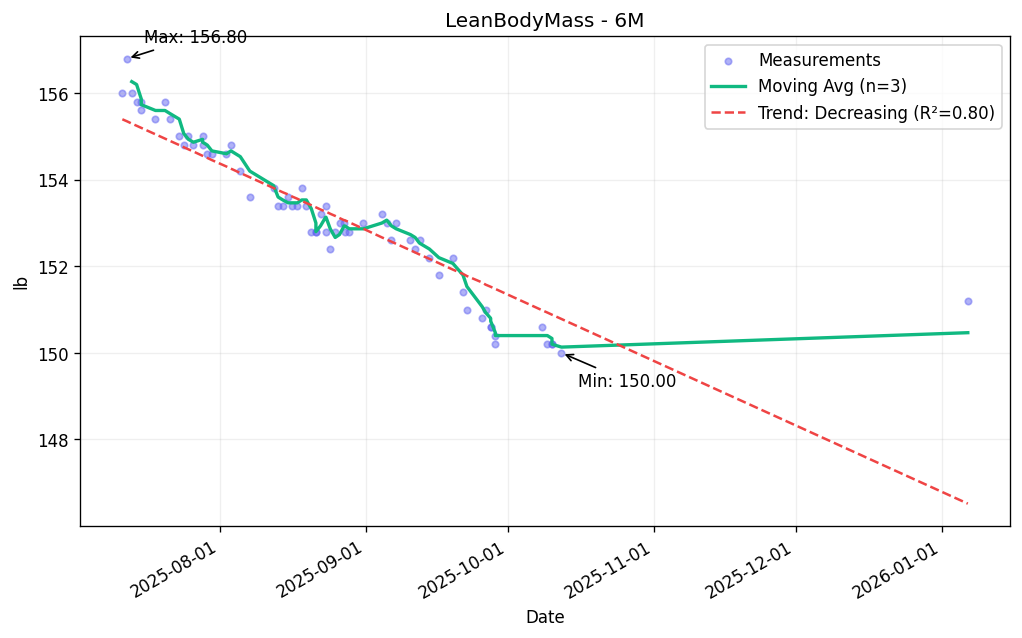
\includegraphics[width=0.95\textwidth]{plots_medical/Vitals_and_Body_Measurements/leanbodymass_6M.png}
\end{figure}
\begin{figure}[H]
\centering
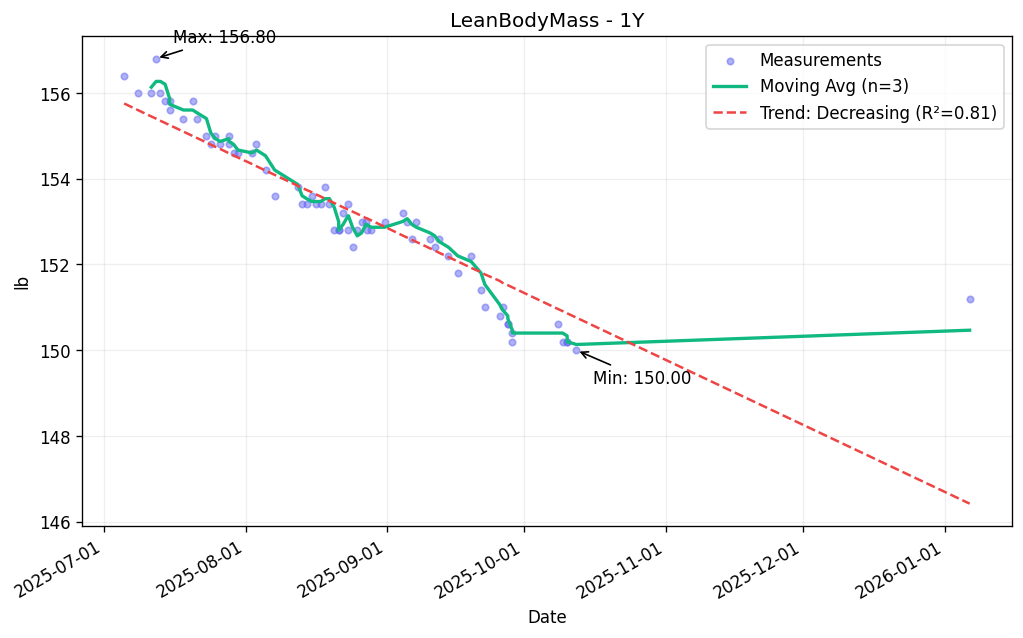
\includegraphics[width=0.95\textwidth]{plots_medical/Vitals_and_Body_Measurements/leanbodymass_1Y.png}
\end{figure}
\begin{figure}[H]
\centering
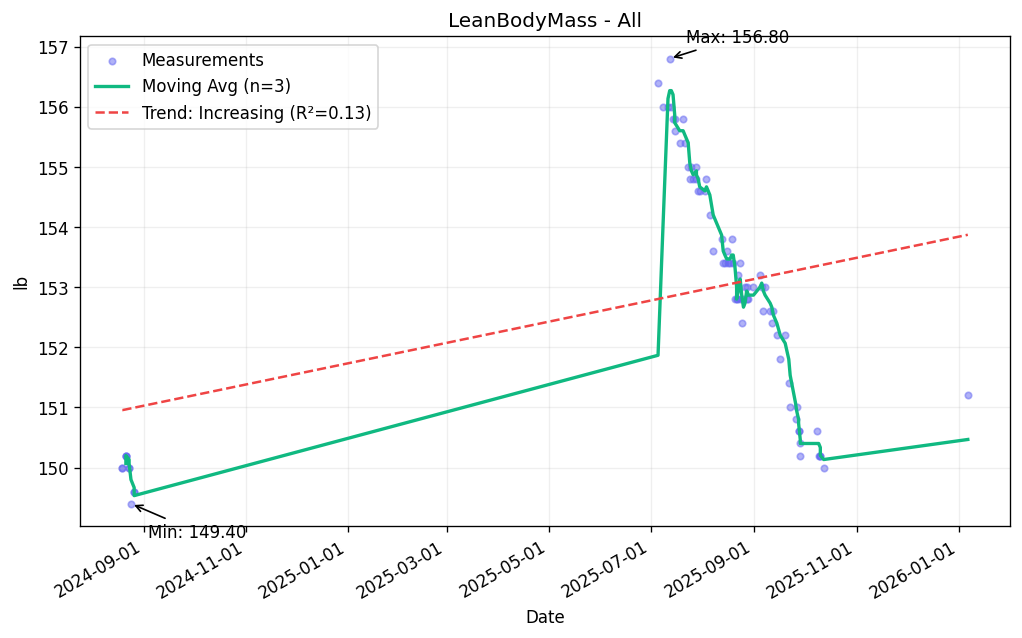
\includegraphics[width=0.95\textwidth]{plots_medical/Vitals_and_Body_Measurements/leanbodymass_All.png}
\end{figure}
\clearpage
\section{Sleep}
\subsection{SleepDurationGoal}
\begin{table}[H]
\centering
\resizebox{\textwidth}{!}{
\begin{tabular}{|l|c|c|c|c|c|c|}
\hline
\textbf{Window} & \textbf{Min} & \textbf{Max} & \textbf{Avg} & \textbf{Start} & \textbf{End} & \textbf{Trend Slope} \\ \hline
1W & - & - & - & - & - & - \\ \hline
1M & - & - & - & - & - & - \\ \hline
3M & - & - & - & - & - & - \\ \hline
6M & - & - & - & - & - & - \\ \hline
1Y & 7.00 hr & 8.00 hr & 7.50 hr & 8.00 & 7.00 & -0.00450 \\ \hline
All & 7.00 hr & 8.50 hr & 7.83 hr & 8.50 & 7.00 & -0.00086 \\ \hline
\end{tabular}
}
\caption{Detailed Statistics for SleepDurationGoal}
\end{table}
\begin{figure}[H]
\centering
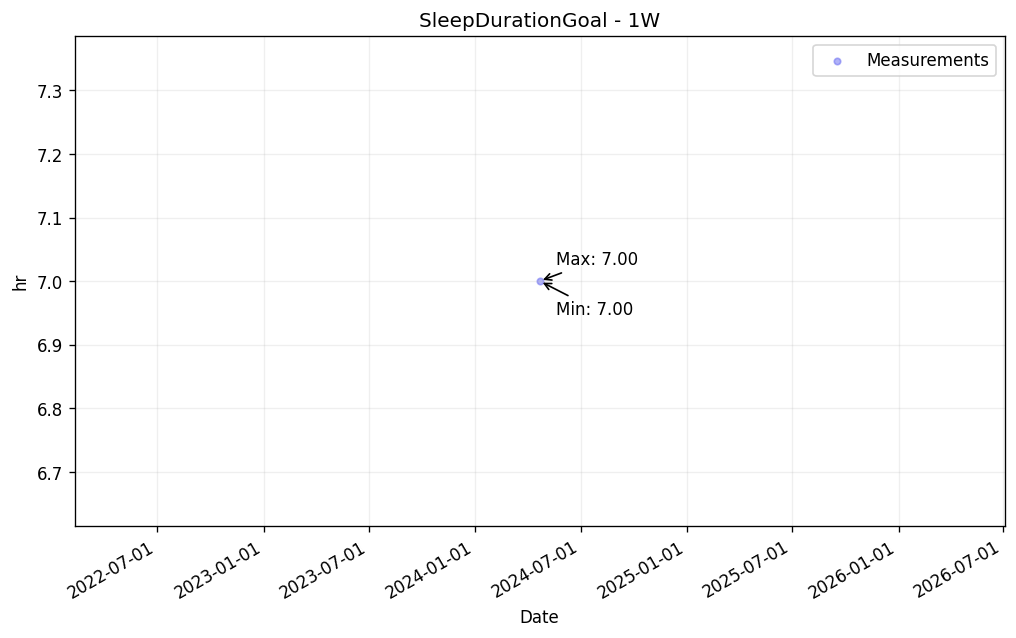
\includegraphics[width=0.95\textwidth]{plots_medical/Sleep/sleepdurationgoal_1W.png}
\end{figure}
\begin{figure}[H]
\centering
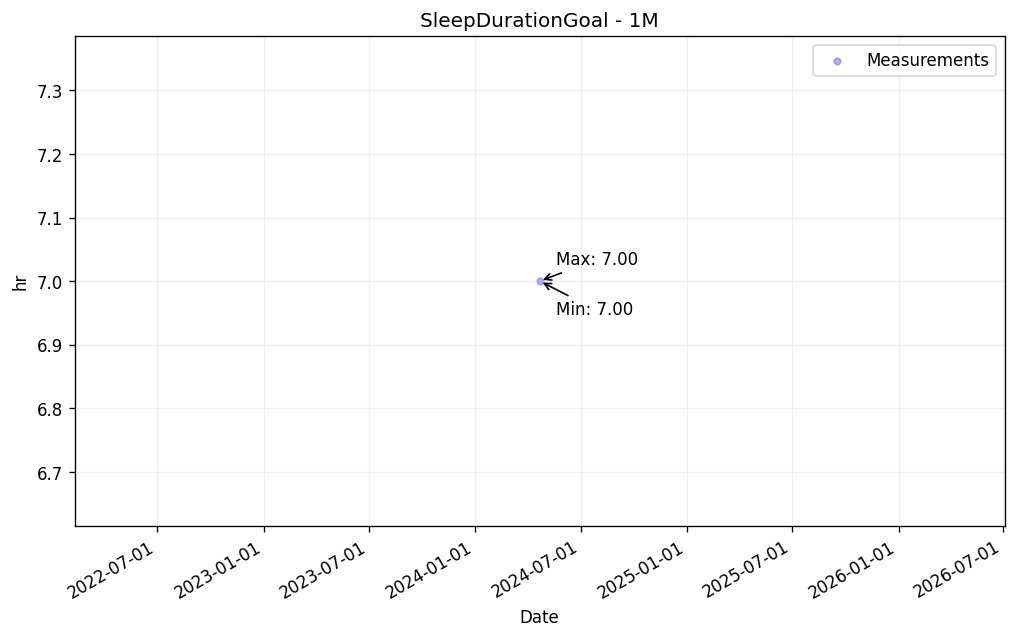
\includegraphics[width=0.95\textwidth]{plots_medical/Sleep/sleepdurationgoal_1M.png}
\end{figure}
\begin{figure}[H]
\centering
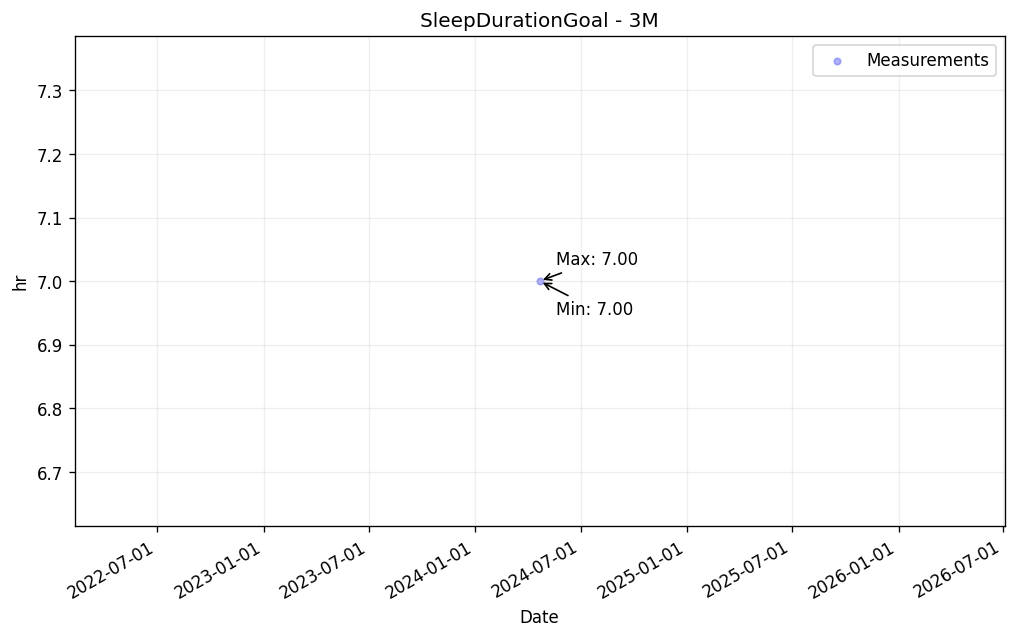
\includegraphics[width=0.95\textwidth]{plots_medical/Sleep/sleepdurationgoal_3M.png}
\end{figure}
\begin{figure}[H]
\centering
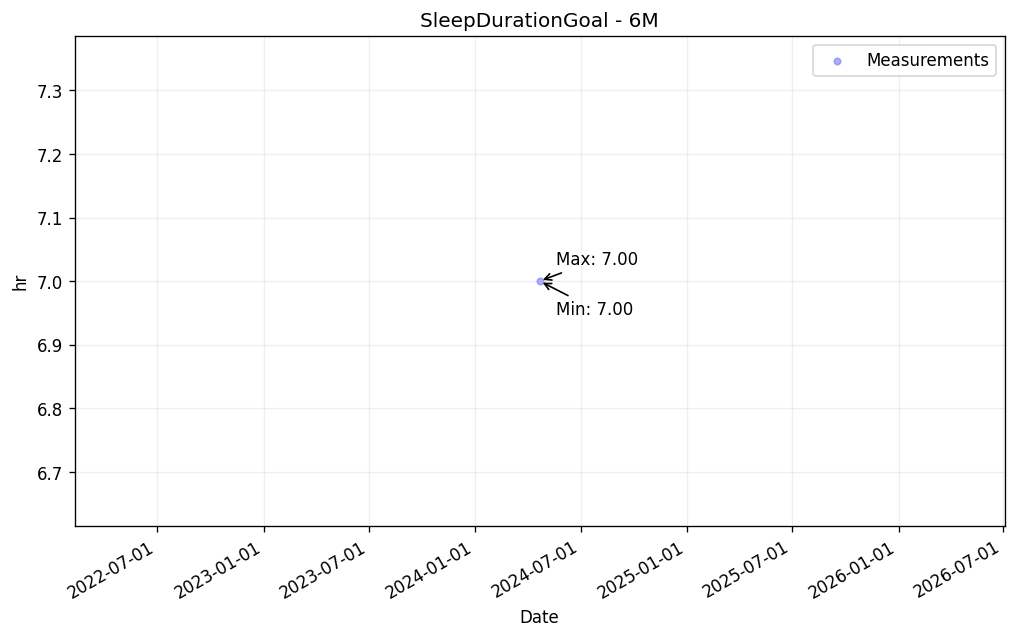
\includegraphics[width=0.95\textwidth]{plots_medical/Sleep/sleepdurationgoal_6M.png}
\end{figure}
\begin{figure}[H]
\centering
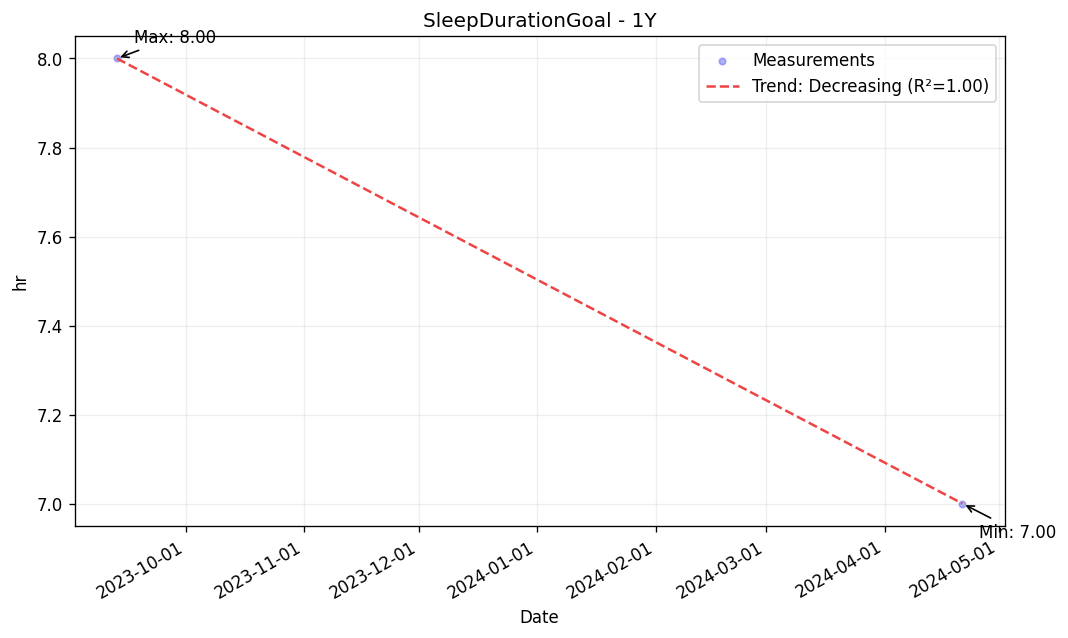
\includegraphics[width=0.95\textwidth]{plots_medical/Sleep/sleepdurationgoal_1Y.png}
\end{figure}
\begin{figure}[H]
\centering
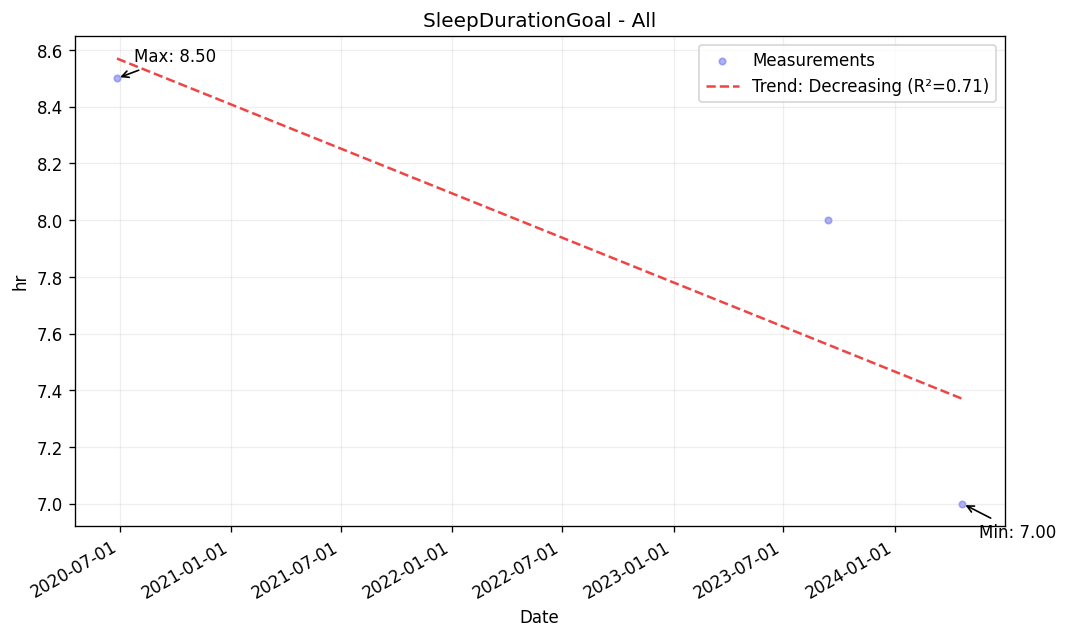
\includegraphics[width=0.95\textwidth]{plots_medical/Sleep/sleepdurationgoal_All.png}
\end{figure}
\clearpage
\section{Activity \& Mobility}
\subsection{ActiveEnergyBurned}
\begin{table}[H]
\centering
\resizebox{\textwidth}{!}{
\begin{tabular}{|l|c|c|c|c|c|c|}
\hline
\textbf{Window} & \textbf{Min} & \textbf{Max} & \textbf{Avg} & \textbf{Start} & \textbf{End} & \textbf{Trend Slope} \\ \hline
1W & 0.00 Cal & 42.55 Cal & 1.36 Cal & 4.68 & 3.36 & -0.07328 \\ \hline
1M & 0.00 Cal & 42.55 Cal & 1.04 Cal & 0.15 & 3.36 & -0.00635 \\ \hline
3M & 0.00 Cal & 63.19 Cal & 0.99 Cal & 0.13 & 3.36 & 0.00083 \\ \hline
6M & 0.00 Cal & 288.97 Cal & 1.16 Cal & 0.16 & 3.36 & -0.01026 \\ \hline
1Y & 0.00 Cal & 425.01 Cal & 1.82 Cal & 2.69 & 3.36 & -0.01136 \\ \hline
All & 0.00 Cal & 641.27 Cal & 2.38 Cal & 9.76 & 3.36 & -0.00366 \\ \hline
\end{tabular}
}
\caption{Detailed Statistics for ActiveEnergyBurned}
\end{table}
\begin{figure}[H]
\centering
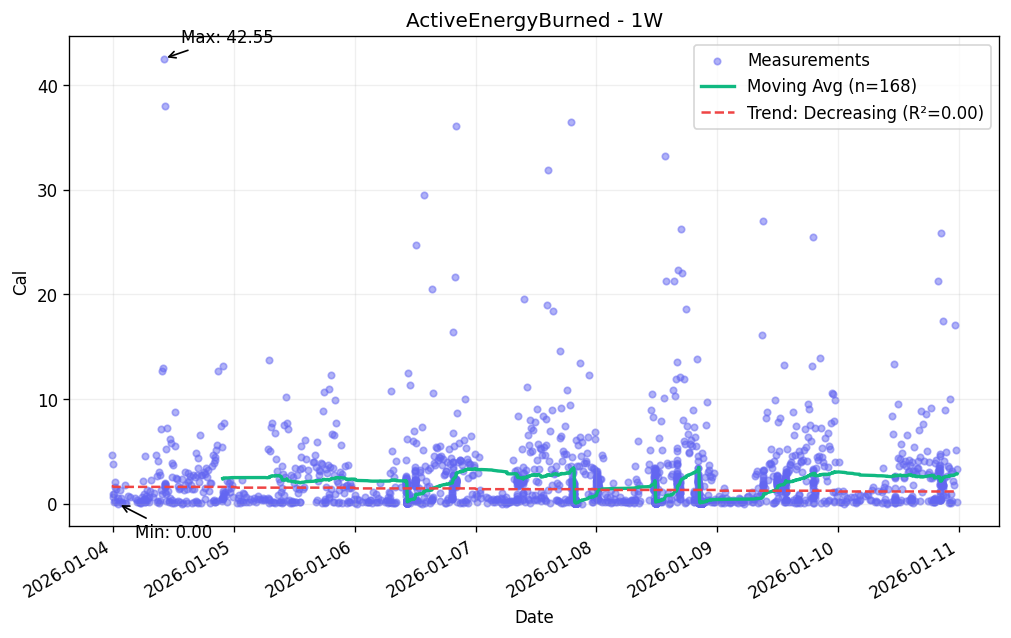
\includegraphics[width=0.95\textwidth]{plots_medical/Activity_and_Mobility/activeenergyburned_1W.png}
\end{figure}
\begin{figure}[H]
\centering
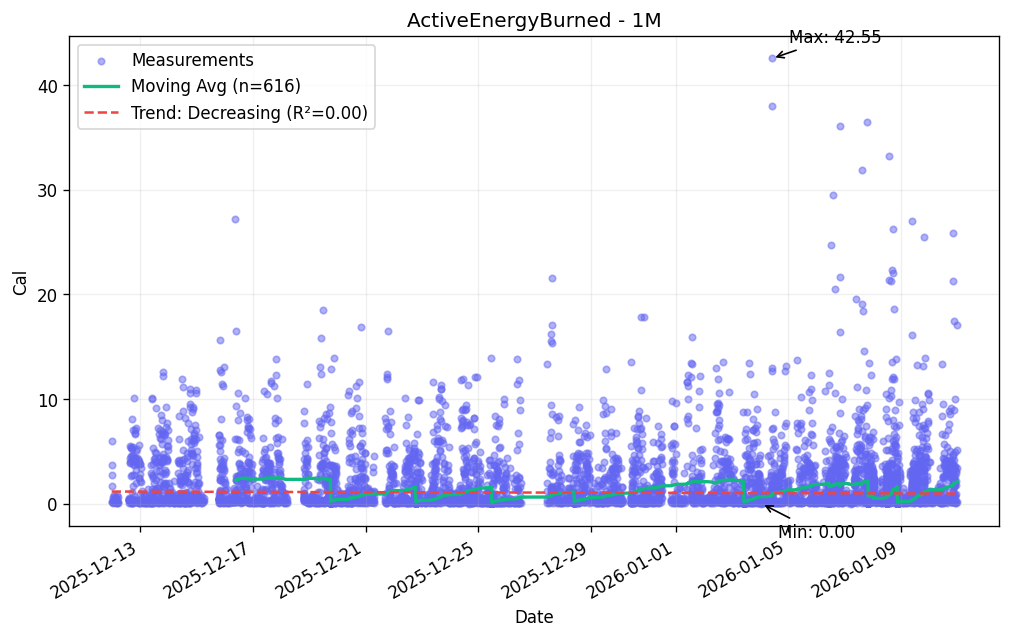
\includegraphics[width=0.95\textwidth]{plots_medical/Activity_and_Mobility/activeenergyburned_1M.png}
\end{figure}
\begin{figure}[H]
\centering
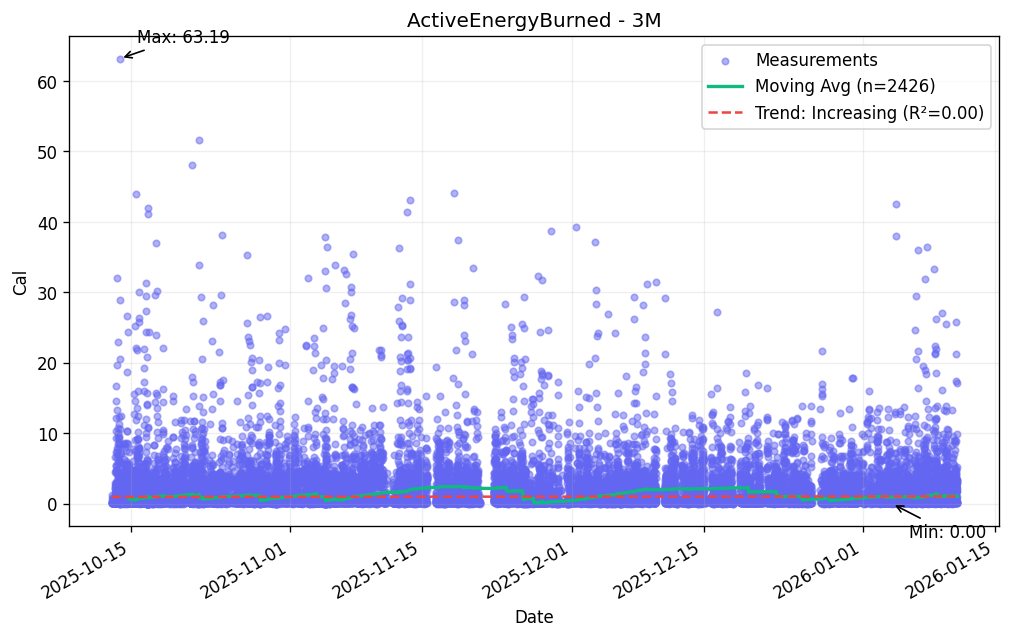
\includegraphics[width=0.95\textwidth]{plots_medical/Activity_and_Mobility/activeenergyburned_3M.png}
\end{figure}
\begin{figure}[H]
\centering
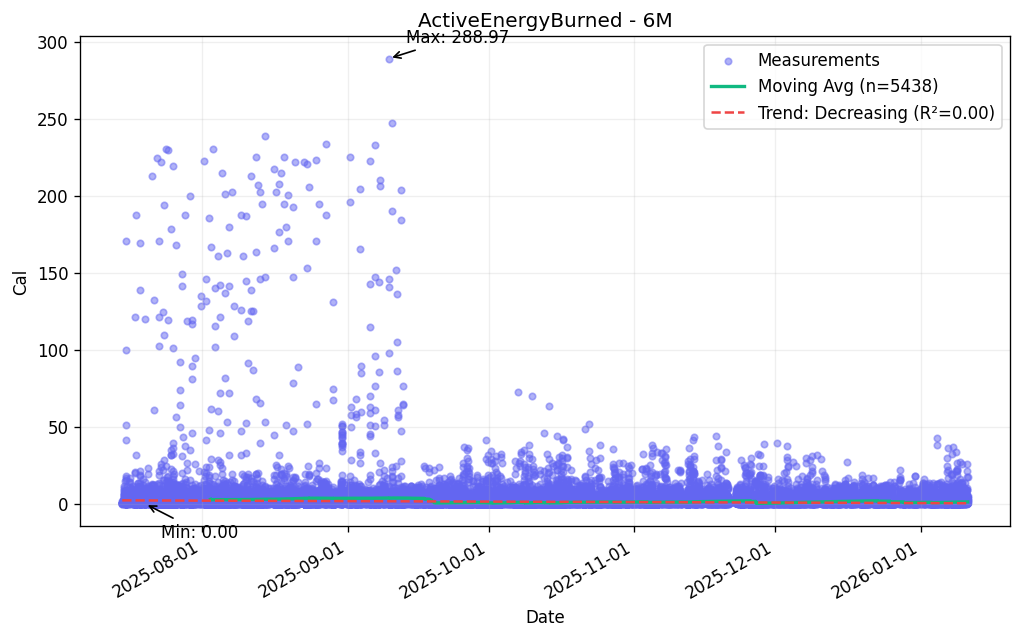
\includegraphics[width=0.95\textwidth]{plots_medical/Activity_and_Mobility/activeenergyburned_6M.png}
\end{figure}
\begin{figure}[H]
\centering
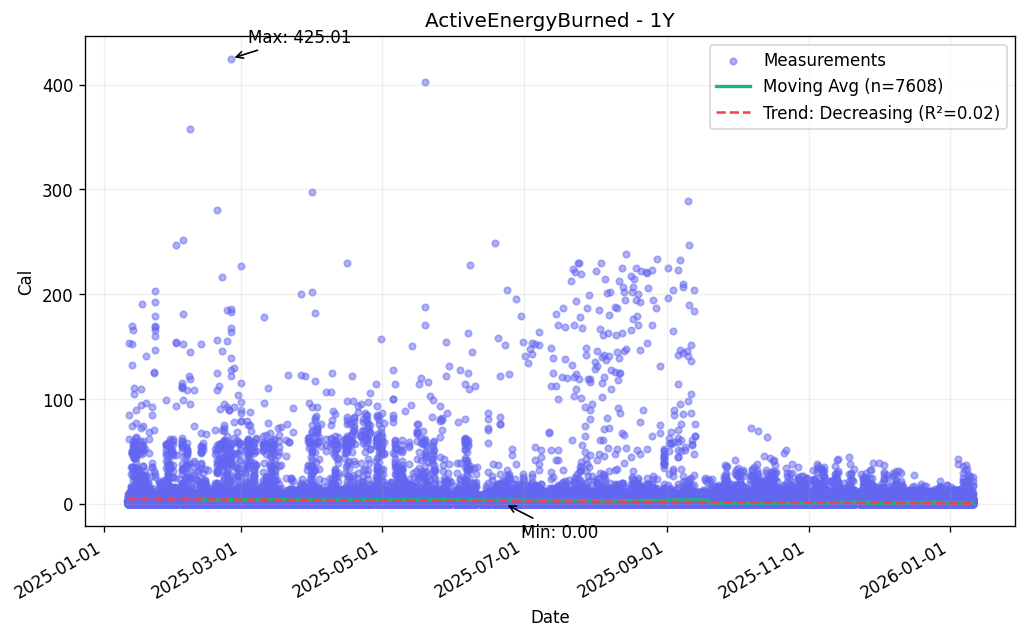
\includegraphics[width=0.95\textwidth]{plots_medical/Activity_and_Mobility/activeenergyburned_1Y.png}
\end{figure}
\begin{figure}[H]
\centering
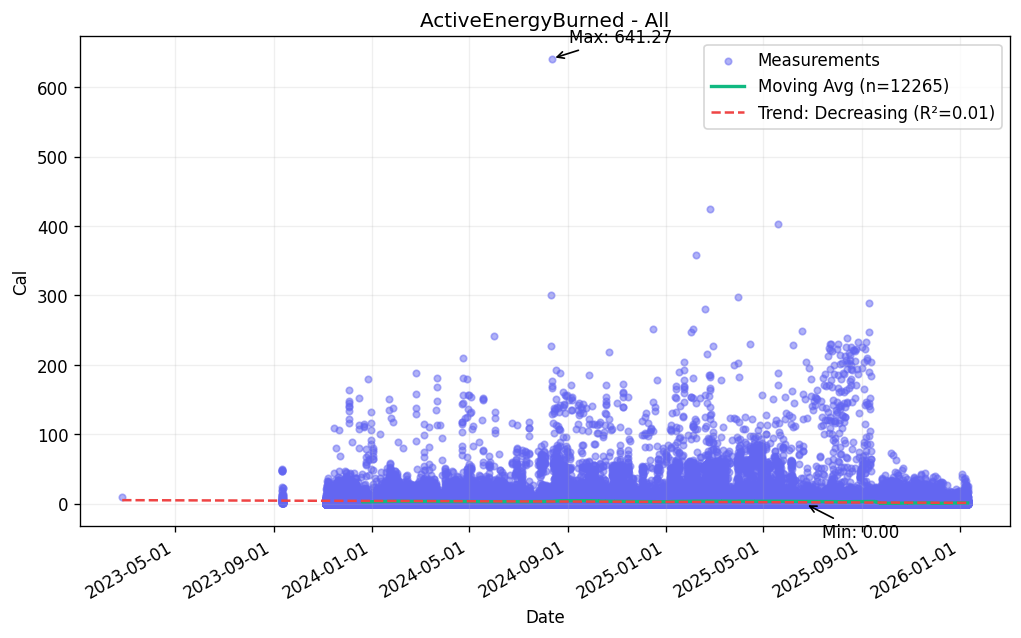
\includegraphics[width=0.95\textwidth]{plots_medical/Activity_and_Mobility/activeenergyburned_All.png}
\end{figure}
\clearpage
\subsection{AppleExerciseTime}
\begin{table}[H]
\centering
\resizebox{\textwidth}{!}{
\begin{tabular}{|l|c|c|c|c|c|c|}
\hline
\textbf{Window} & \textbf{Min} & \textbf{Max} & \textbf{Avg} & \textbf{Start} & \textbf{End} & \textbf{Trend Slope} \\ \hline
1W & 1.00 min & 1.00 min & 1.00 min & 1.00 & 1.00 & 0.00000 \\ \hline
1M & 1.00 min & 1.00 min & 1.00 min & 1.00 & 1.00 & 0.00000 \\ \hline
3M & 1.00 min & 1.00 min & 1.00 min & 1.00 & 1.00 & 0.00000 \\ \hline
6M & 1.00 min & 1.00 min & 1.00 min & 1.00 & 1.00 & 0.00000 \\ \hline
1Y & 1.00 min & 1.00 min & 1.00 min & 1.00 & 1.00 & 0.00000 \\ \hline
All & 1.00 min & 1.00 min & 1.00 min & 1.00 & 1.00 & 0.00000 \\ \hline
\end{tabular}
}
\caption{Detailed Statistics for AppleExerciseTime}
\end{table}
\begin{figure}[H]
\centering
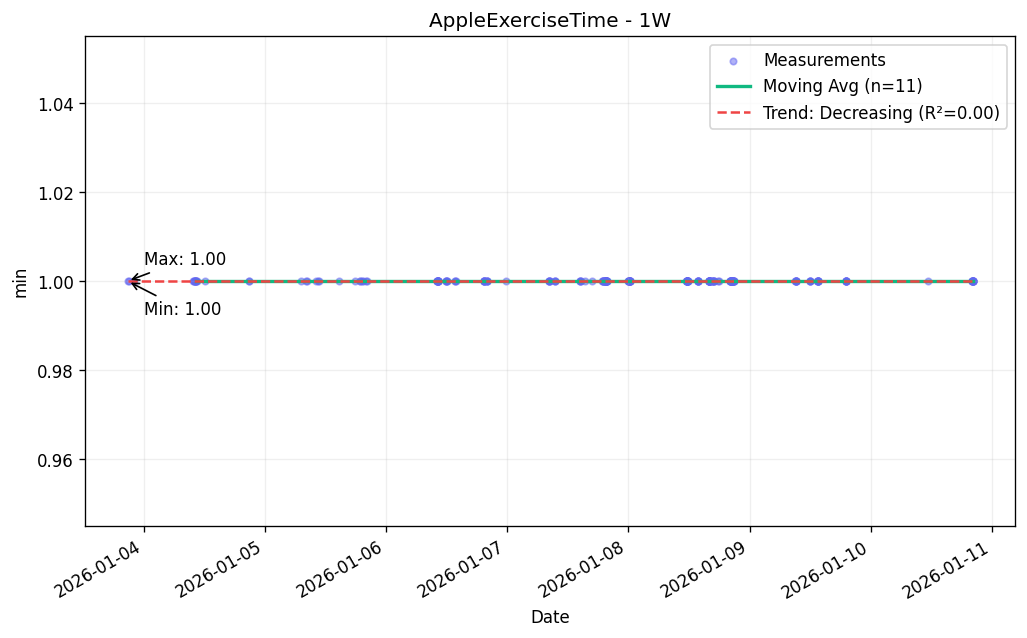
\includegraphics[width=0.95\textwidth]{plots_medical/Activity_and_Mobility/appleexercisetime_1W.png}
\end{figure}
\begin{figure}[H]
\centering
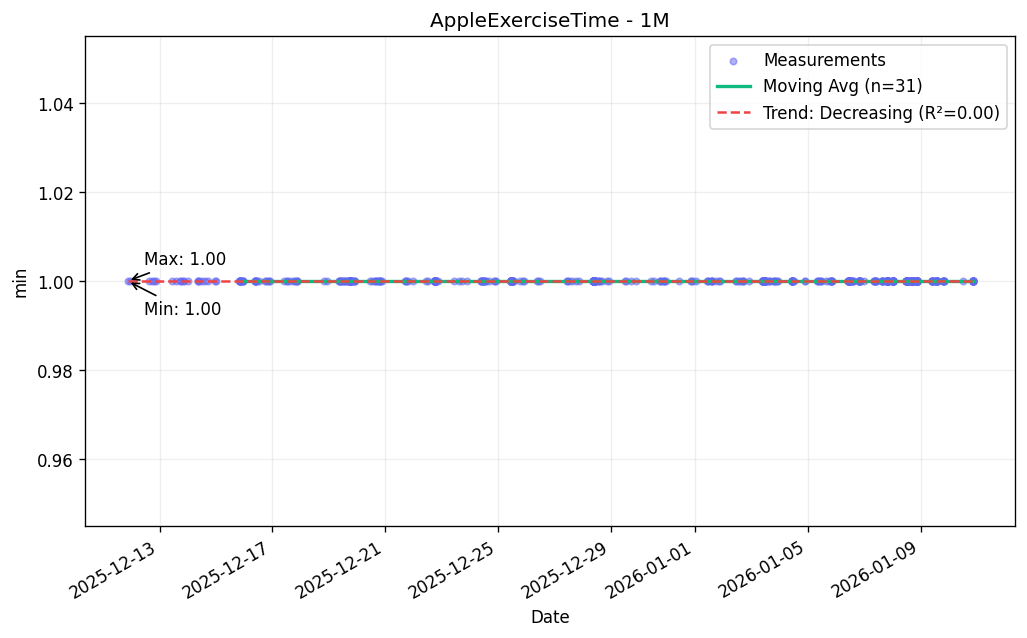
\includegraphics[width=0.95\textwidth]{plots_medical/Activity_and_Mobility/appleexercisetime_1M.png}
\end{figure}
\begin{figure}[H]
\centering
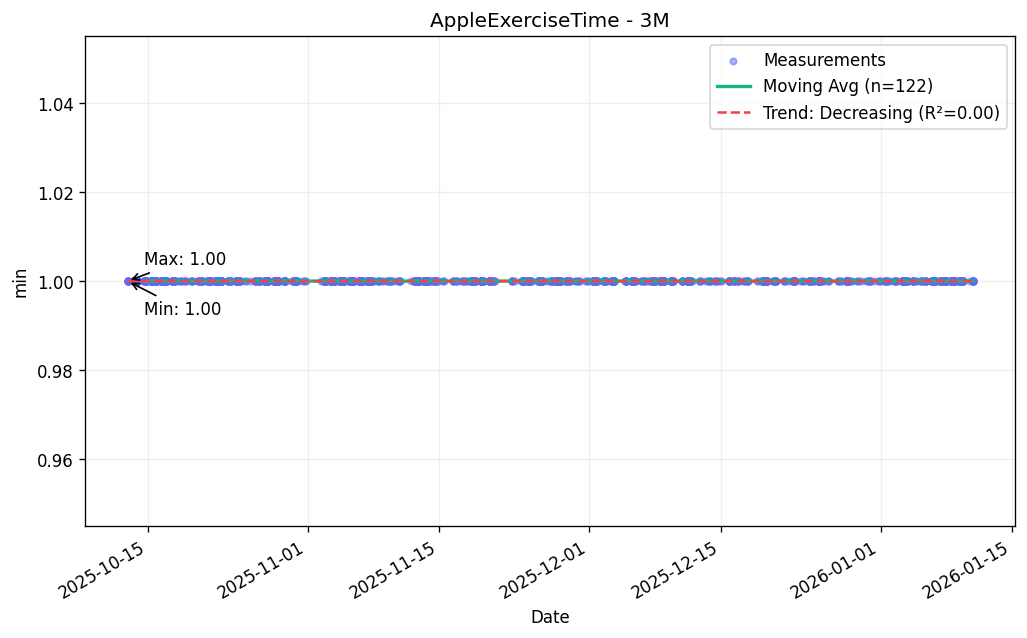
\includegraphics[width=0.95\textwidth]{plots_medical/Activity_and_Mobility/appleexercisetime_3M.png}
\end{figure}
\begin{figure}[H]
\centering
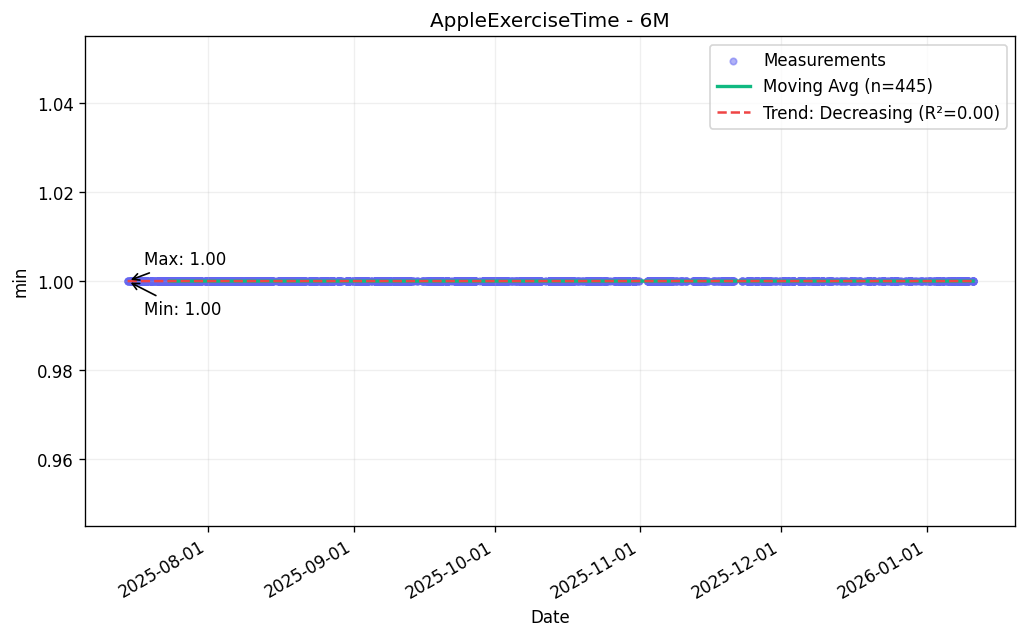
\includegraphics[width=0.95\textwidth]{plots_medical/Activity_and_Mobility/appleexercisetime_6M.png}
\end{figure}
\begin{figure}[H]
\centering
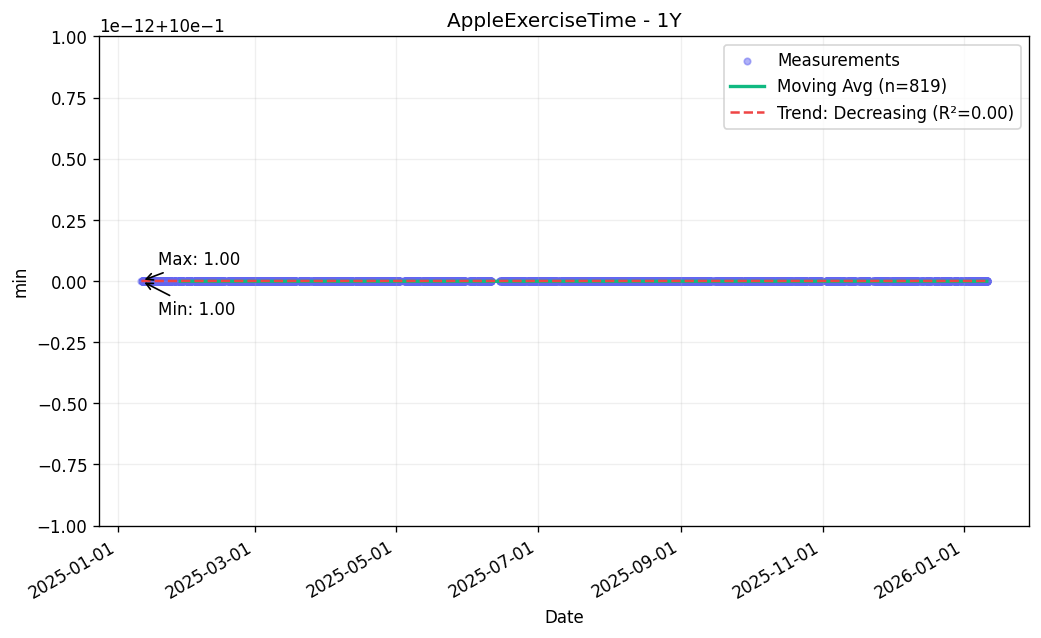
\includegraphics[width=0.95\textwidth]{plots_medical/Activity_and_Mobility/appleexercisetime_1Y.png}
\end{figure}
\begin{figure}[H]
\centering
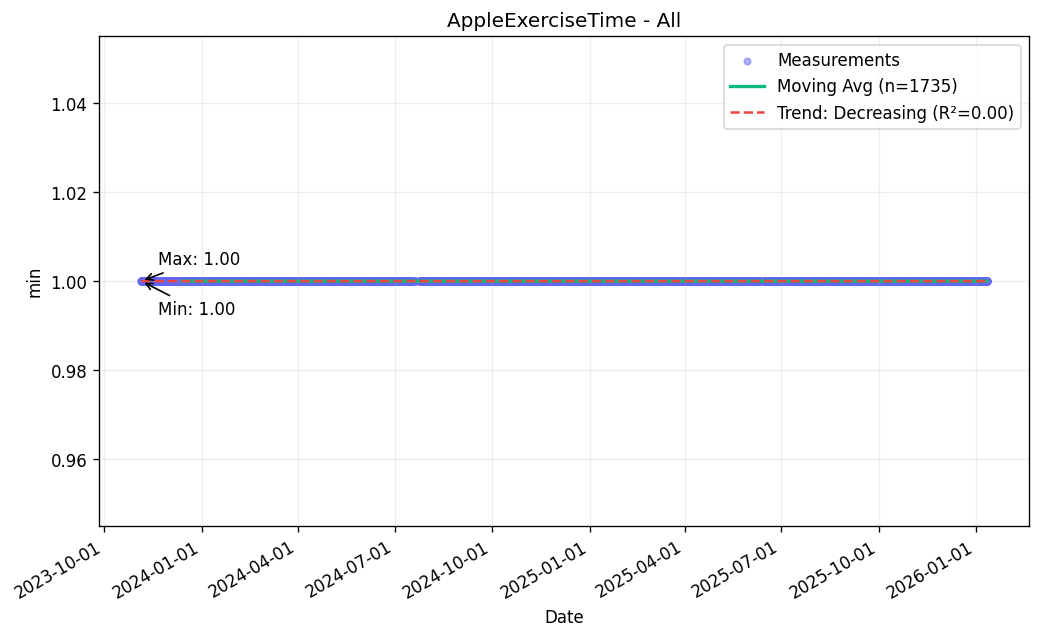
\includegraphics[width=0.95\textwidth]{plots_medical/Activity_and_Mobility/appleexercisetime_All.png}
\end{figure}
\clearpage
\subsection{DistanceWalkingRunning}
\begin{table}[H]
\centering
\resizebox{\textwidth}{!}{
\begin{tabular}{|l|c|c|c|c|c|c|}
\hline
\textbf{Window} & \textbf{Min} & \textbf{Max} & \textbf{Avg} & \textbf{Start} & \textbf{End} & \textbf{Trend Slope} \\ \hline
1W & 0.00 mi & 0.51 mi & 0.02 mi & 0.01 & 0.02 & -0.00111 \\ \hline
1M & 0.00 mi & 0.51 mi & 0.01 mi & 0.04 & 0.02 & 0.00022 \\ \hline
3M & 0.00 mi & 0.52 mi & 0.02 mi & 0.01 & 0.02 & -0.00007 \\ \hline
6M & 0.00 mi & 0.53 mi & 0.01 mi & 0.01 & 0.02 & 0.00005 \\ \hline
1Y & 0.00 mi & 3.54 mi & 0.02 mi & 0.01 & 0.02 & -0.00012 \\ \hline
All & 0.00 mi & 3.54 mi & 0.03 mi & 0.02 & 0.02 & -0.00002 \\ \hline
\end{tabular}
}
\caption{Detailed Statistics for DistanceWalkingRunning}
\end{table}
\begin{figure}[H]
\centering
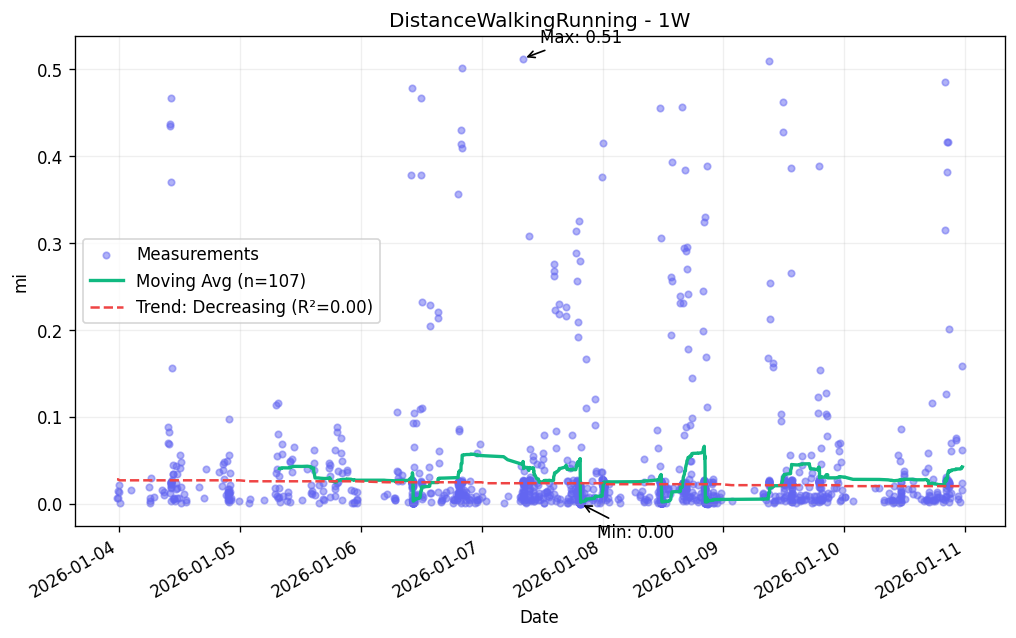
\includegraphics[width=0.95\textwidth]{plots_medical/Activity_and_Mobility/distancewalkingrunning_1W.png}
\end{figure}
\begin{figure}[H]
\centering
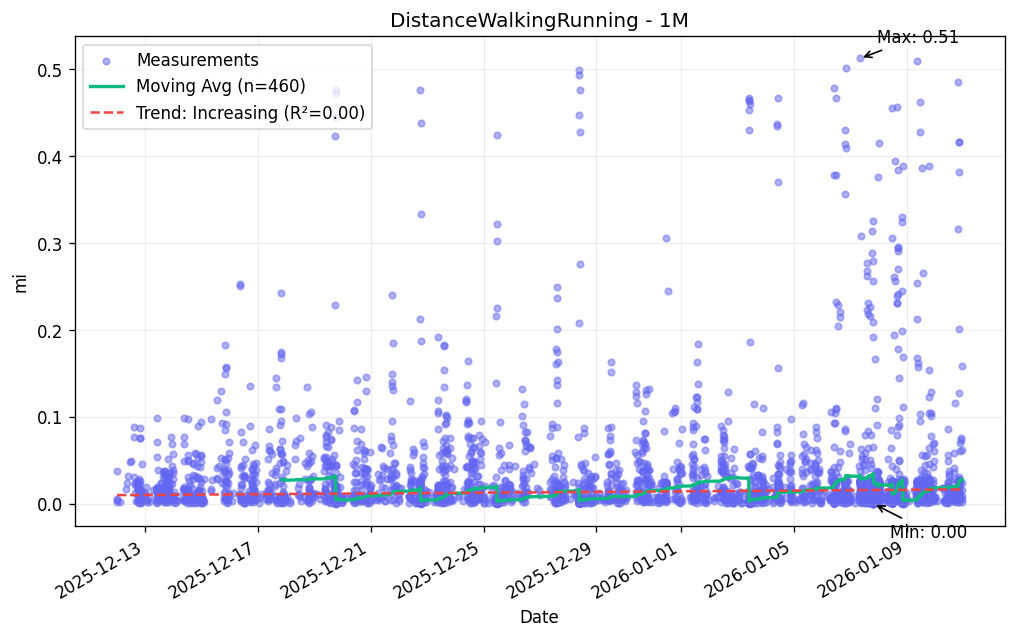
\includegraphics[width=0.95\textwidth]{plots_medical/Activity_and_Mobility/distancewalkingrunning_1M.png}
\end{figure}
\begin{figure}[H]
\centering
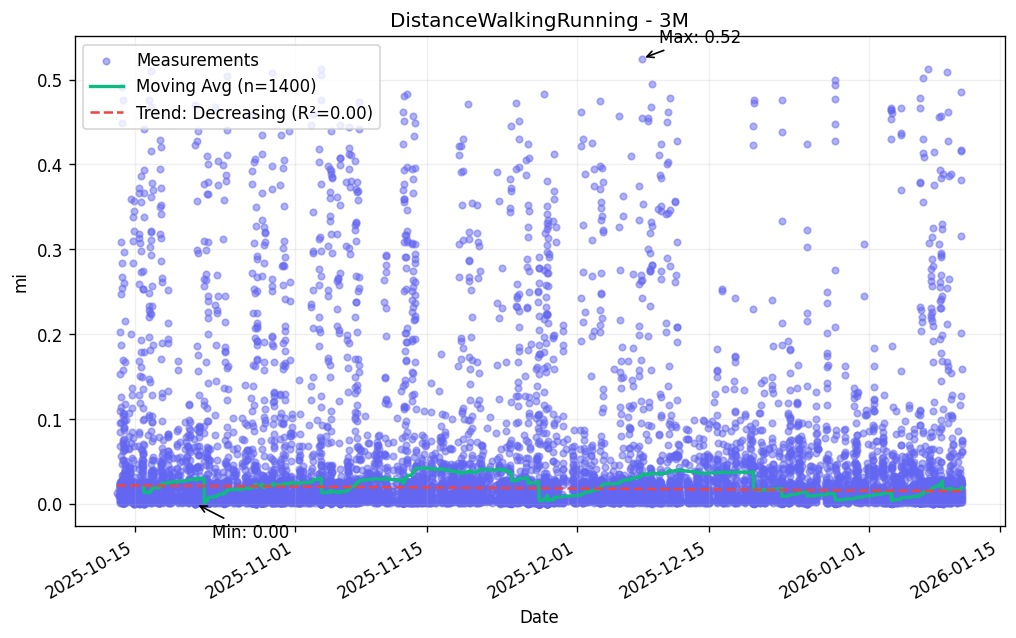
\includegraphics[width=0.95\textwidth]{plots_medical/Activity_and_Mobility/distancewalkingrunning_3M.png}
\end{figure}
\begin{figure}[H]
\centering
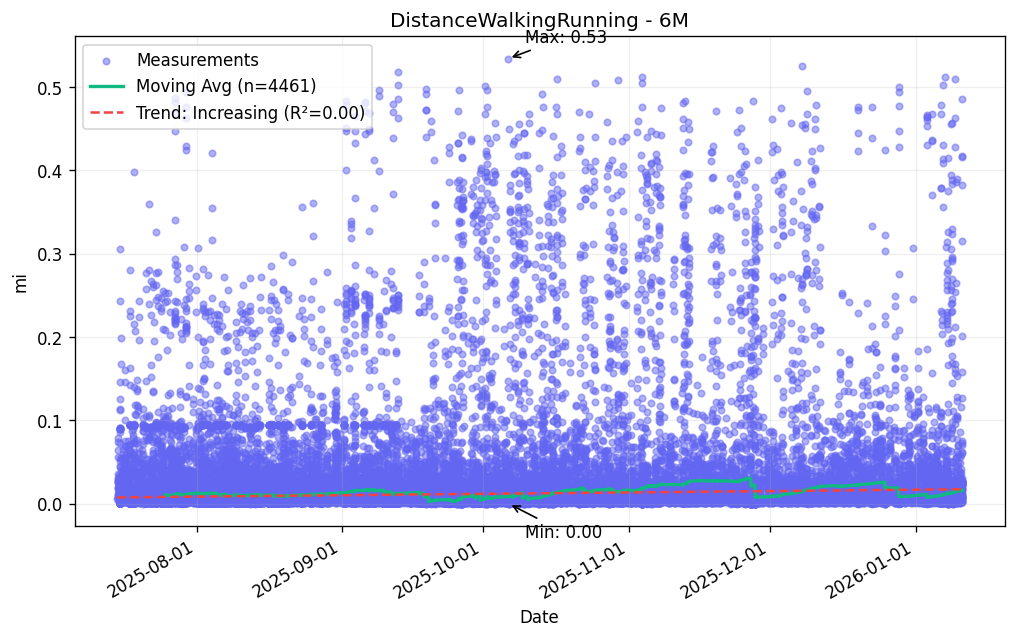
\includegraphics[width=0.95\textwidth]{plots_medical/Activity_and_Mobility/distancewalkingrunning_6M.png}
\end{figure}
\begin{figure}[H]
\centering
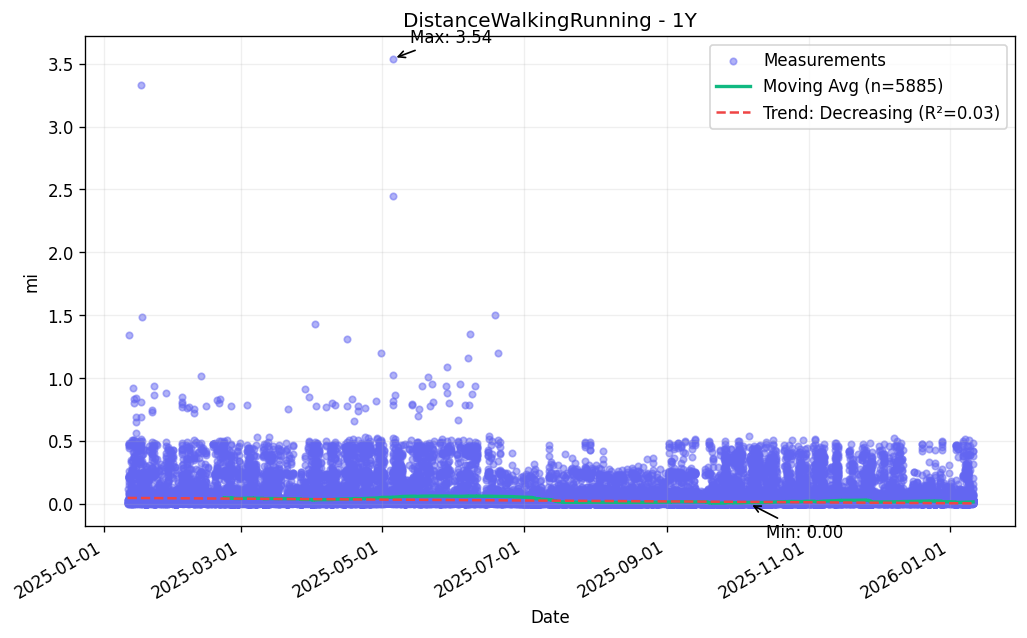
\includegraphics[width=0.95\textwidth]{plots_medical/Activity_and_Mobility/distancewalkingrunning_1Y.png}
\end{figure}
\begin{figure}[H]
\centering
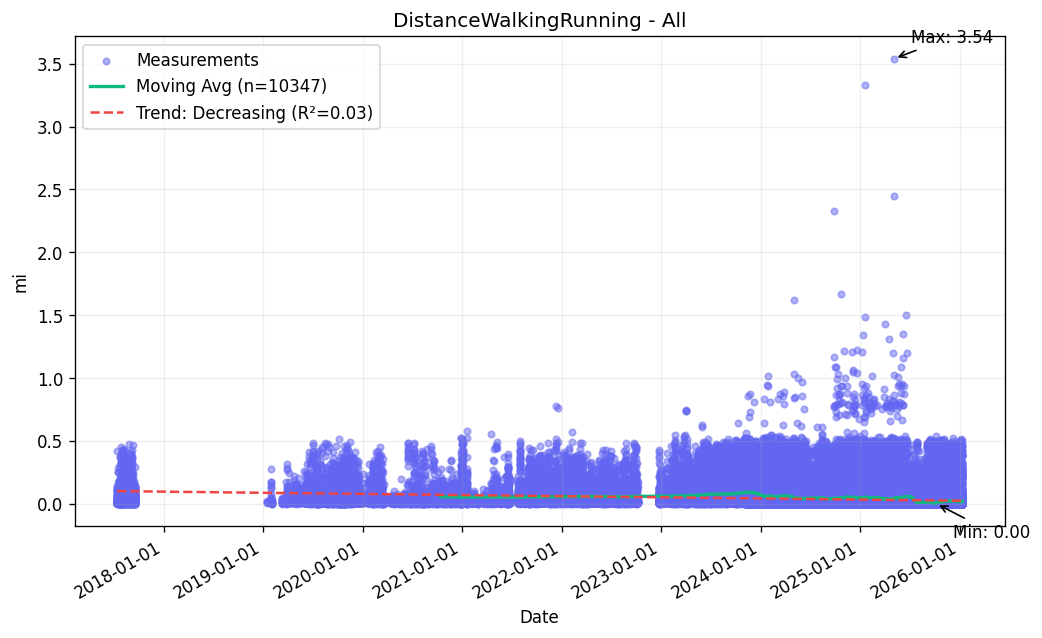
\includegraphics[width=0.95\textwidth]{plots_medical/Activity_and_Mobility/distancewalkingrunning_All.png}
\end{figure}
\clearpage
\subsection{FlightsClimbed}
\begin{table}[H]
\centering
\resizebox{\textwidth}{!}{
\begin{tabular}{|l|c|c|c|c|c|c|}
\hline
\textbf{Window} & \textbf{Min} & \textbf{Max} & \textbf{Avg} & \textbf{Start} & \textbf{End} & \textbf{Trend Slope} \\ \hline
1W & 1.00 count & 4.00 count & 1.27 count & 1.00 & 1.00 & 0.07661 \\ \hline
1M & 1.00 count & 4.00 count & 1.17 count & 1.00 & 1.00 & 0.00930 \\ \hline
3M & 1.00 count & 14.00 count & 1.23 count & 1.00 & 1.00 & -0.00087 \\ \hline
6M & 1.00 count & 21.00 count & 1.20 count & 1.00 & 1.00 & 0.00100 \\ \hline
1Y & 1.00 count & 21.00 count & 1.18 count & 1.00 & 1.00 & 0.00038 \\ \hline
All & 1.00 count & 21.00 count & 1.24 count & 2.00 & 1.00 & 0.00001 \\ \hline
\end{tabular}
}
\caption{Detailed Statistics for FlightsClimbed}
\end{table}
\begin{figure}[H]
\centering
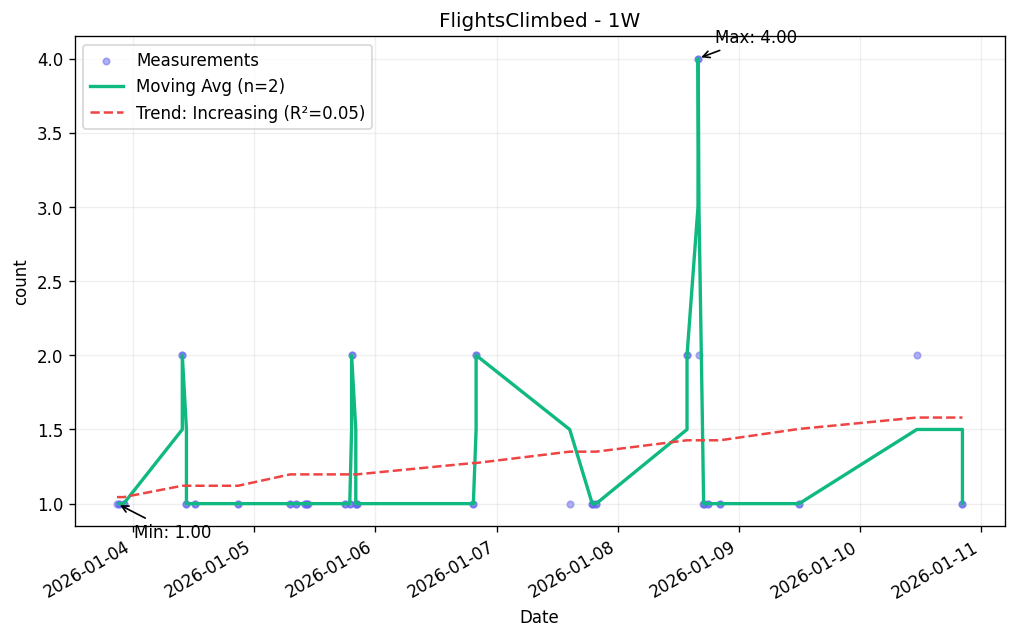
\includegraphics[width=0.95\textwidth]{plots_medical/Activity_and_Mobility/flightsclimbed_1W.png}
\end{figure}
\begin{figure}[H]
\centering
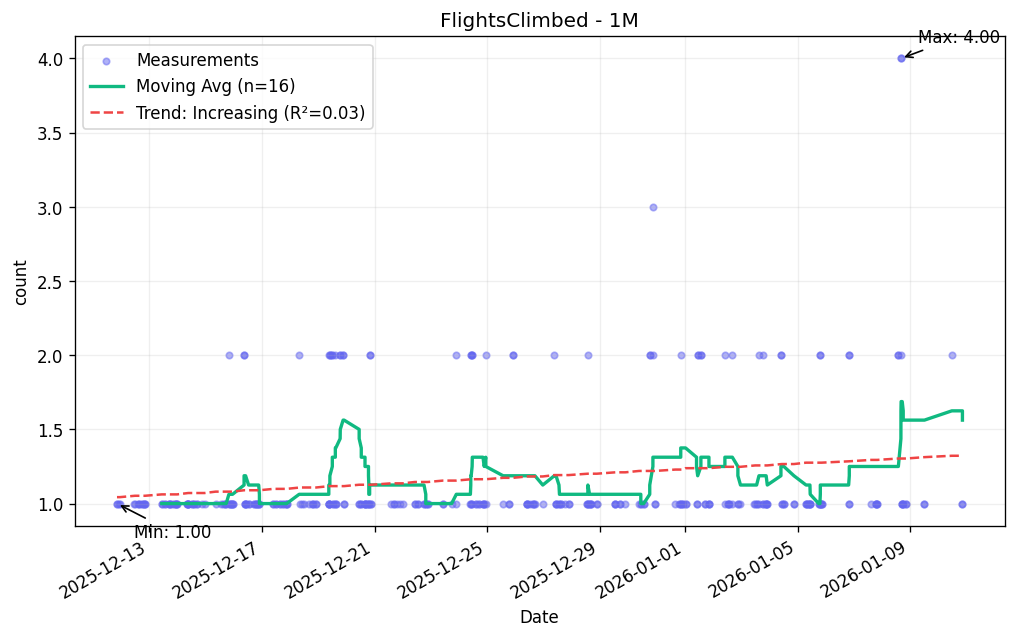
\includegraphics[width=0.95\textwidth]{plots_medical/Activity_and_Mobility/flightsclimbed_1M.png}
\end{figure}
\begin{figure}[H]
\centering
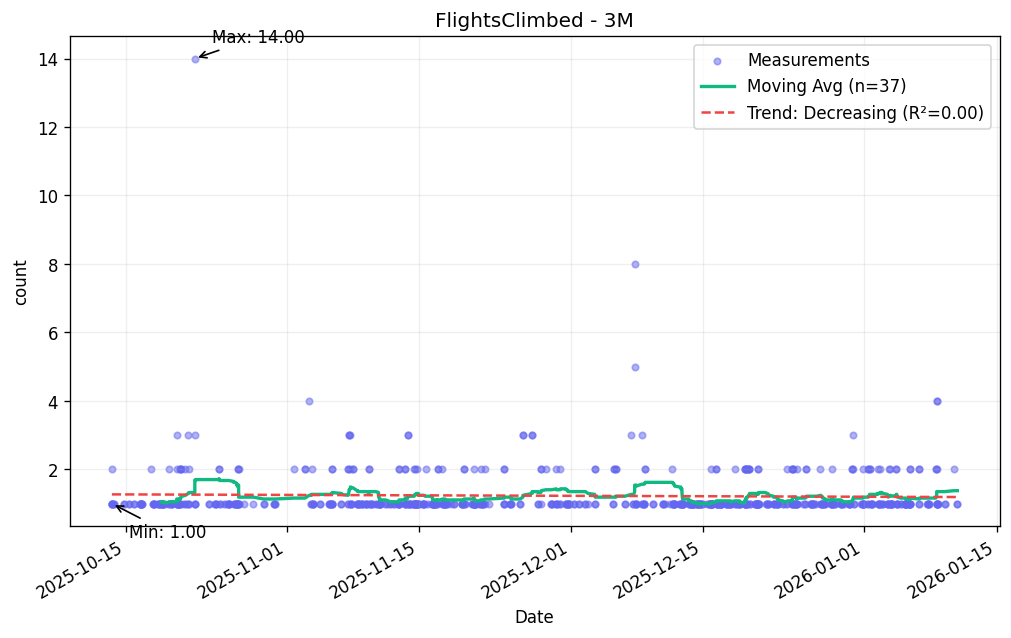
\includegraphics[width=0.95\textwidth]{plots_medical/Activity_and_Mobility/flightsclimbed_3M.png}
\end{figure}
\begin{figure}[H]
\centering
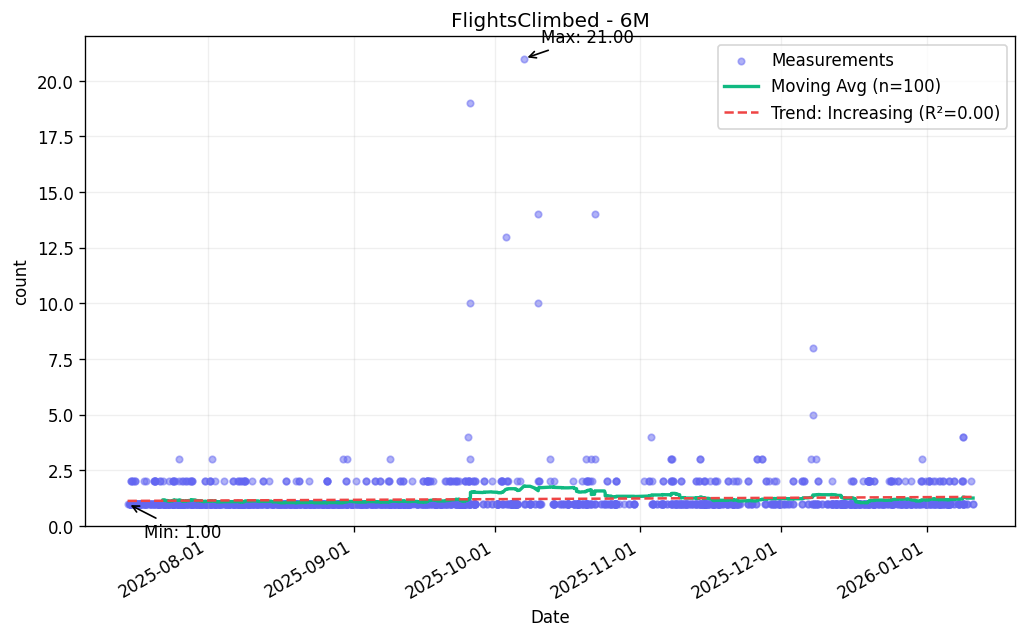
\includegraphics[width=0.95\textwidth]{plots_medical/Activity_and_Mobility/flightsclimbed_6M.png}
\end{figure}
\begin{figure}[H]
\centering
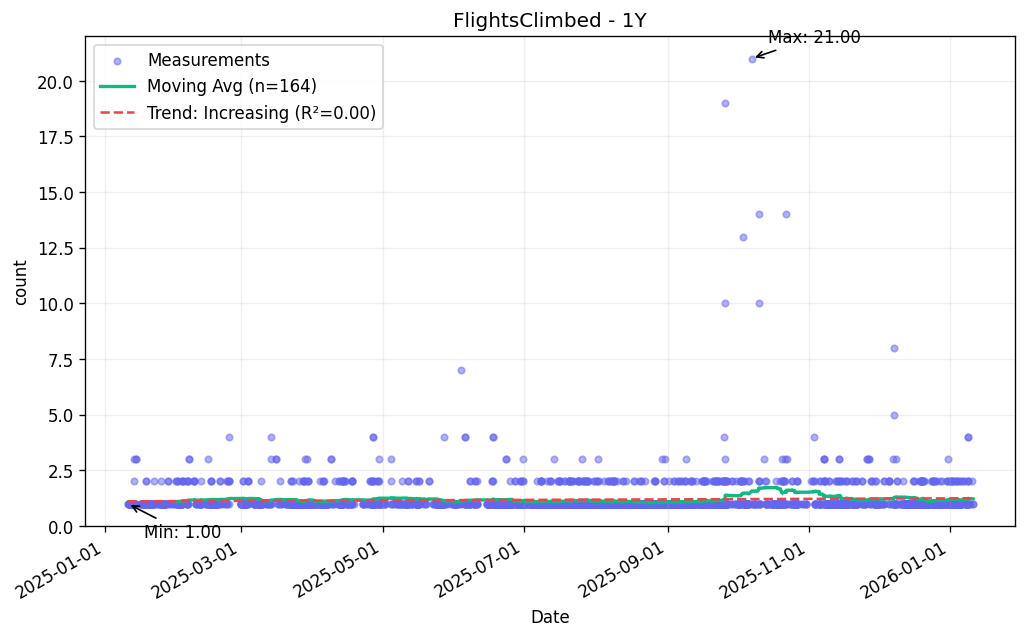
\includegraphics[width=0.95\textwidth]{plots_medical/Activity_and_Mobility/flightsclimbed_1Y.png}
\end{figure}
\begin{figure}[H]
\centering
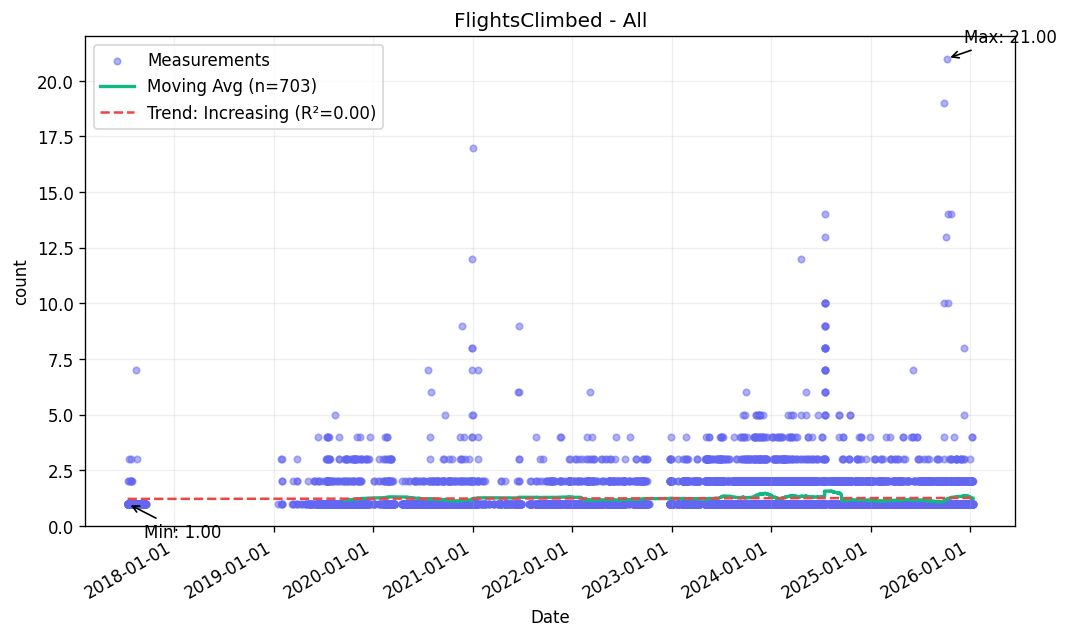
\includegraphics[width=0.95\textwidth]{plots_medical/Activity_and_Mobility/flightsclimbed_All.png}
\end{figure}
\clearpage
\subsection{RunningGroundContactTime}
\begin{table}[H]
\centering
\resizebox{\textwidth}{!}{
\begin{tabular}{|l|c|c|c|c|c|c|}
\hline
\textbf{Window} & \textbf{Min} & \textbf{Max} & \textbf{Avg} & \textbf{Start} & \textbf{End} & \textbf{Trend Slope} \\ \hline
1W & 266.00 ms & 290.14 ms & 274.46 ms & 266.00 & 290.14 & 17.63900 \\ \hline
1M & 266.00 ms & 290.14 ms & 274.46 ms & 266.00 & 290.14 & 17.63900 \\ \hline
3M & 266.00 ms & 290.14 ms & 274.46 ms & 266.00 & 290.14 & 17.63900 \\ \hline
6M & 266.00 ms & 290.14 ms & 274.46 ms & 266.00 & 290.14 & 17.63900 \\ \hline
1Y & 266.00 ms & 290.14 ms & 274.46 ms & 266.00 & 290.14 & 17.63900 \\ \hline
All & 266.00 ms & 290.14 ms & 274.46 ms & 266.00 & 290.14 & 17.63900 \\ \hline
\end{tabular}
}
\caption{Detailed Statistics for RunningGroundContactTime}
\end{table}
\begin{figure}[H]
\centering
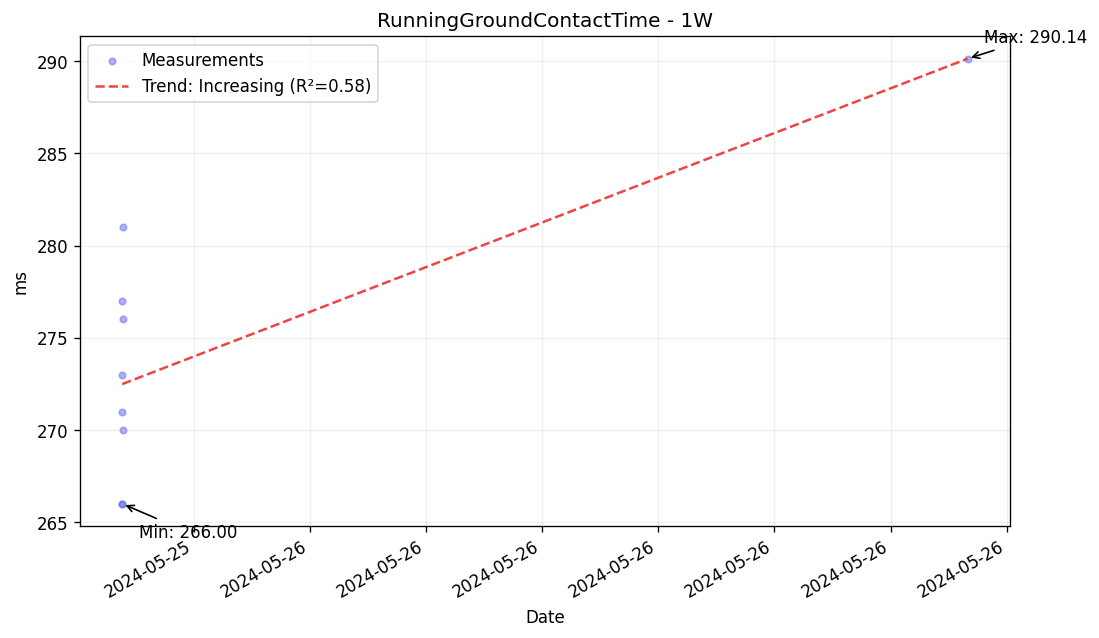
\includegraphics[width=0.95\textwidth]{plots_medical/Activity_and_Mobility/runninggroundcontacttime_1W.png}
\end{figure}
\begin{figure}[H]
\centering
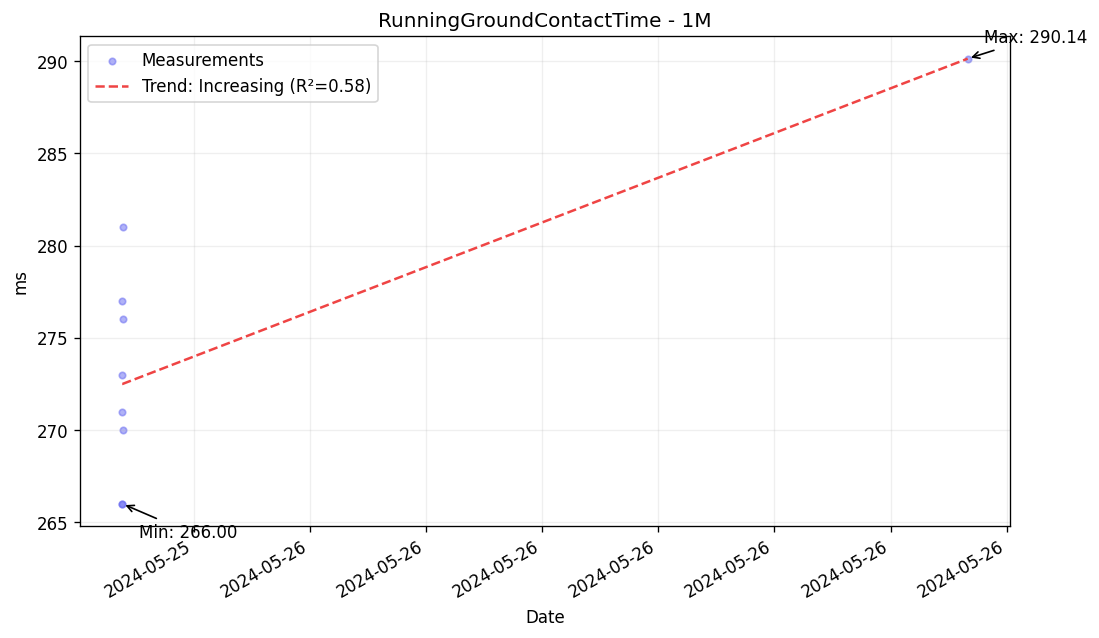
\includegraphics[width=0.95\textwidth]{plots_medical/Activity_and_Mobility/runninggroundcontacttime_1M.png}
\end{figure}
\begin{figure}[H]
\centering
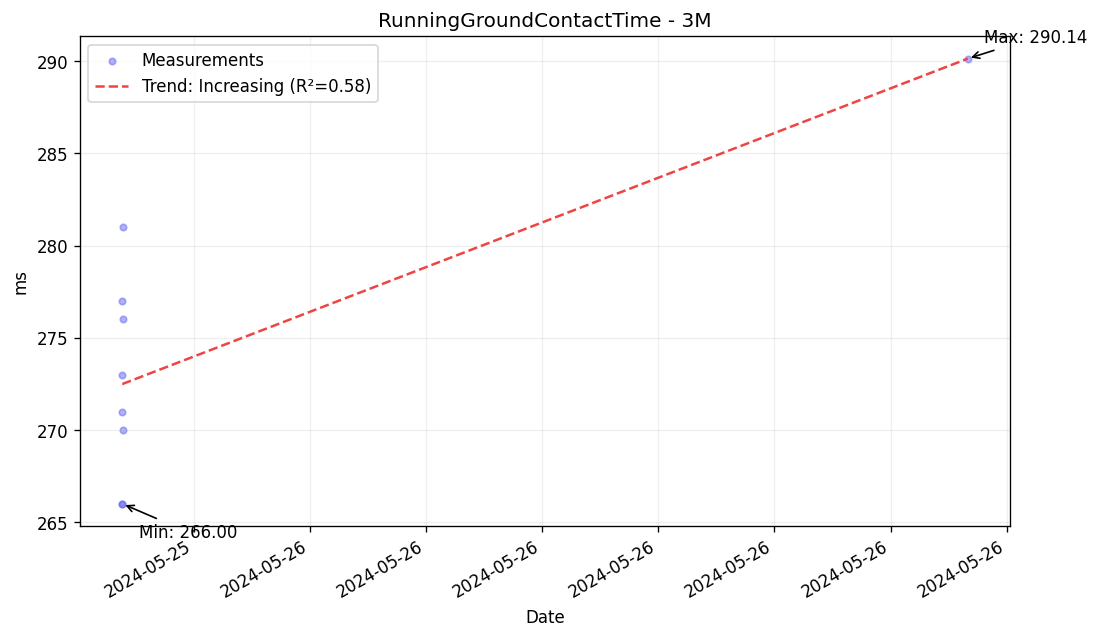
\includegraphics[width=0.95\textwidth]{plots_medical/Activity_and_Mobility/runninggroundcontacttime_3M.png}
\end{figure}
\begin{figure}[H]
\centering
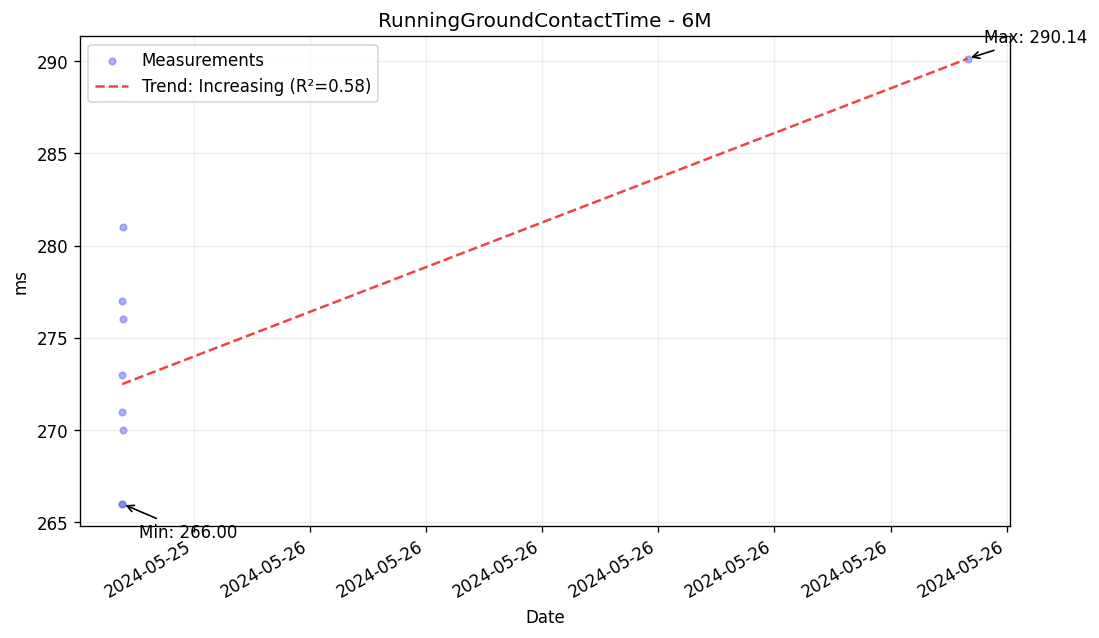
\includegraphics[width=0.95\textwidth]{plots_medical/Activity_and_Mobility/runninggroundcontacttime_6M.png}
\end{figure}
\begin{figure}[H]
\centering
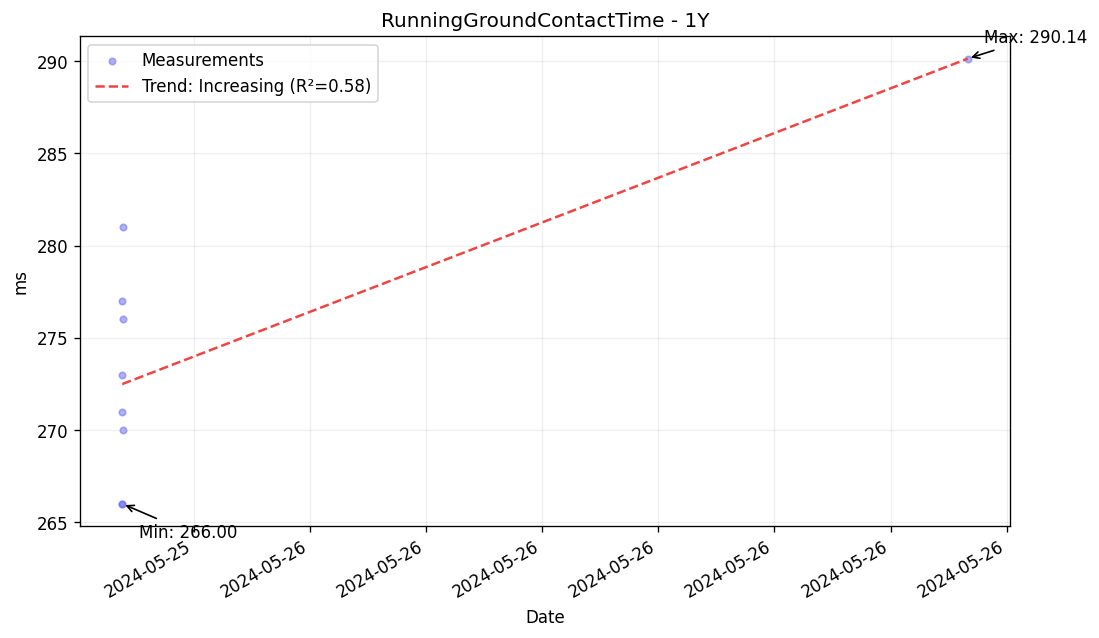
\includegraphics[width=0.95\textwidth]{plots_medical/Activity_and_Mobility/runninggroundcontacttime_1Y.png}
\end{figure}
\begin{figure}[H]
\centering
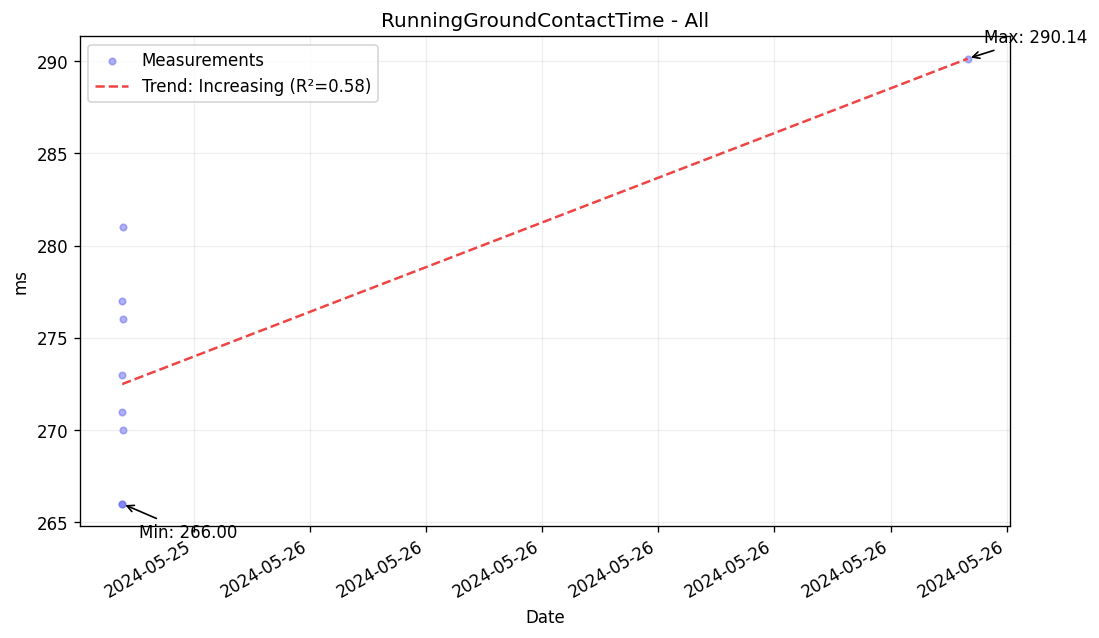
\includegraphics[width=0.95\textwidth]{plots_medical/Activity_and_Mobility/runninggroundcontacttime_All.png}
\end{figure}
\clearpage
\subsection{RunningPower}
\begin{table}[H]
\centering
\resizebox{\textwidth}{!}{
\begin{tabular}{|l|c|c|c|c|c|c|}
\hline
\textbf{Window} & \textbf{Min} & \textbf{Max} & \textbf{Avg} & \textbf{Start} & \textbf{End} & \textbf{Trend Slope} \\ \hline
1W & 62.00 W & 226.00 W & 106.45 W & 85.00 & 92.33 & 4.31991 \\ \hline
1M & 62.00 W & 226.00 W & 106.45 W & 85.00 & 92.33 & 4.31991 \\ \hline
3M & 62.00 W & 226.00 W & 106.45 W & 85.00 & 92.33 & 4.31991 \\ \hline
6M & 62.00 W & 226.00 W & 106.45 W & 85.00 & 92.33 & 4.31991 \\ \hline
1Y & 62.00 W & 226.00 W & 106.45 W & 85.00 & 92.33 & 4.31991 \\ \hline
All & 62.00 W & 355.00 W & 126.60 W & 88.00 & 92.33 & -0.24086 \\ \hline
\end{tabular}
}
\caption{Detailed Statistics for RunningPower}
\end{table}
\begin{figure}[H]
\centering
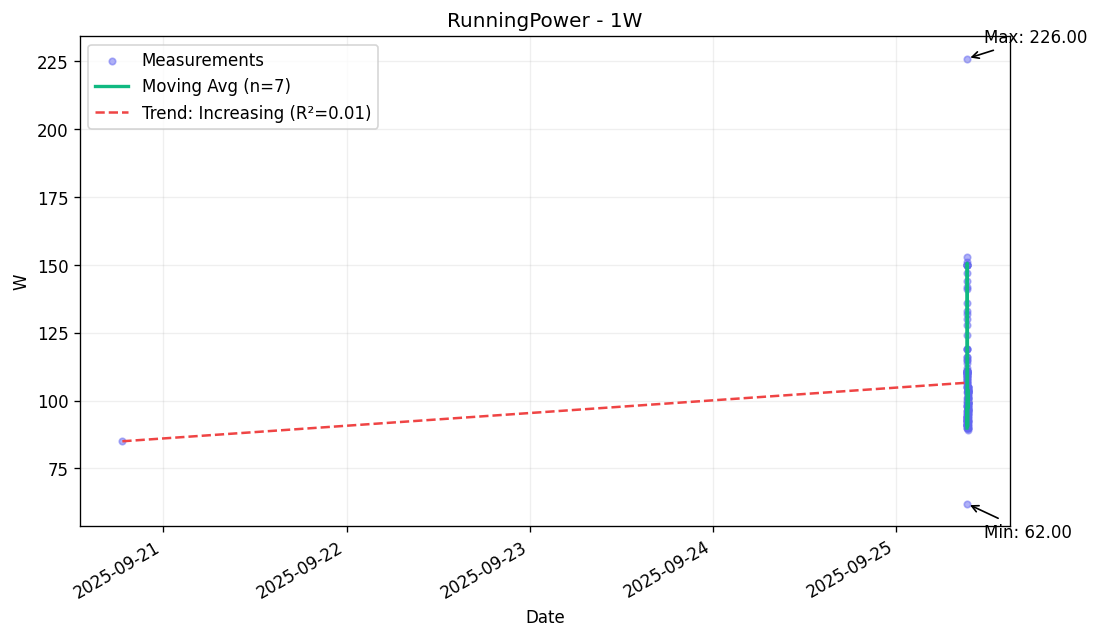
\includegraphics[width=0.95\textwidth]{plots_medical/Activity_and_Mobility/runningpower_1W.png}
\end{figure}
\begin{figure}[H]
\centering
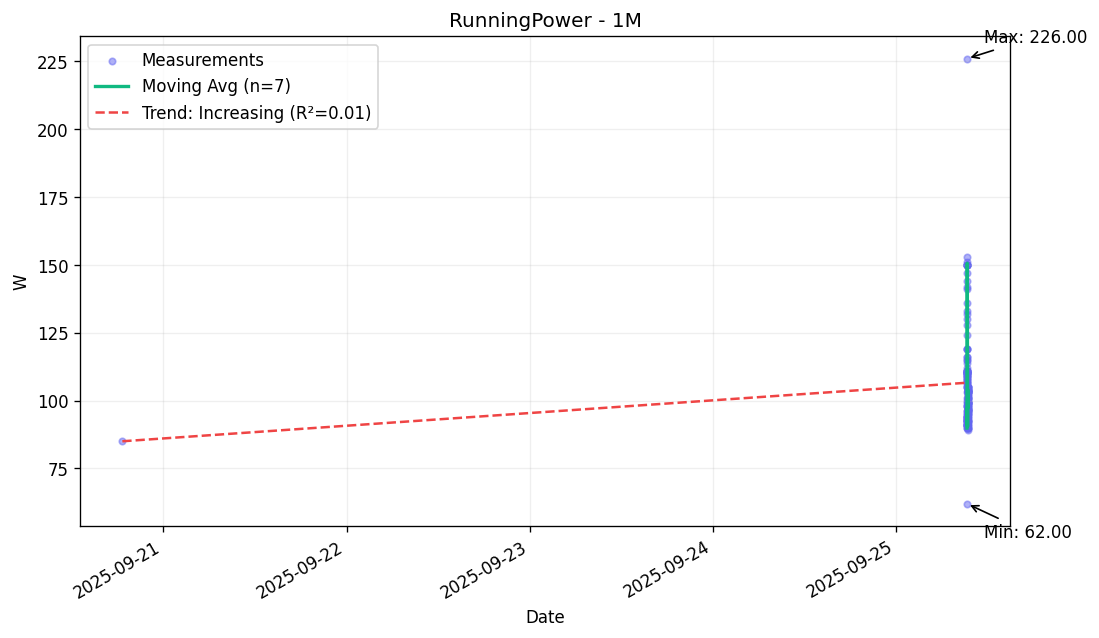
\includegraphics[width=0.95\textwidth]{plots_medical/Activity_and_Mobility/runningpower_1M.png}
\end{figure}
\begin{figure}[H]
\centering
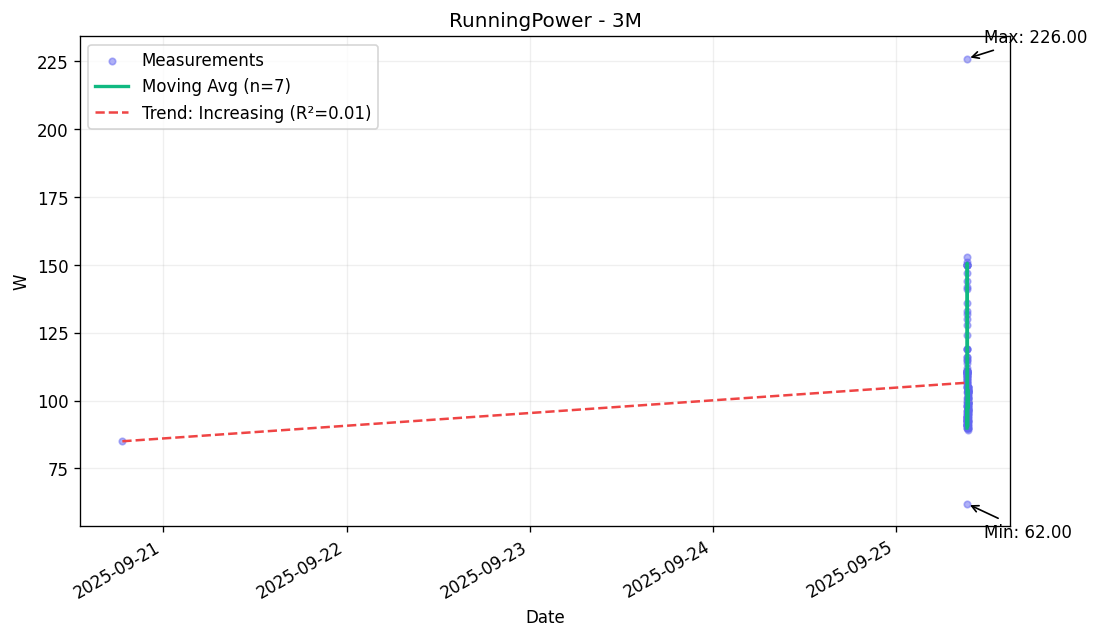
\includegraphics[width=0.95\textwidth]{plots_medical/Activity_and_Mobility/runningpower_3M.png}
\end{figure}
\begin{figure}[H]
\centering
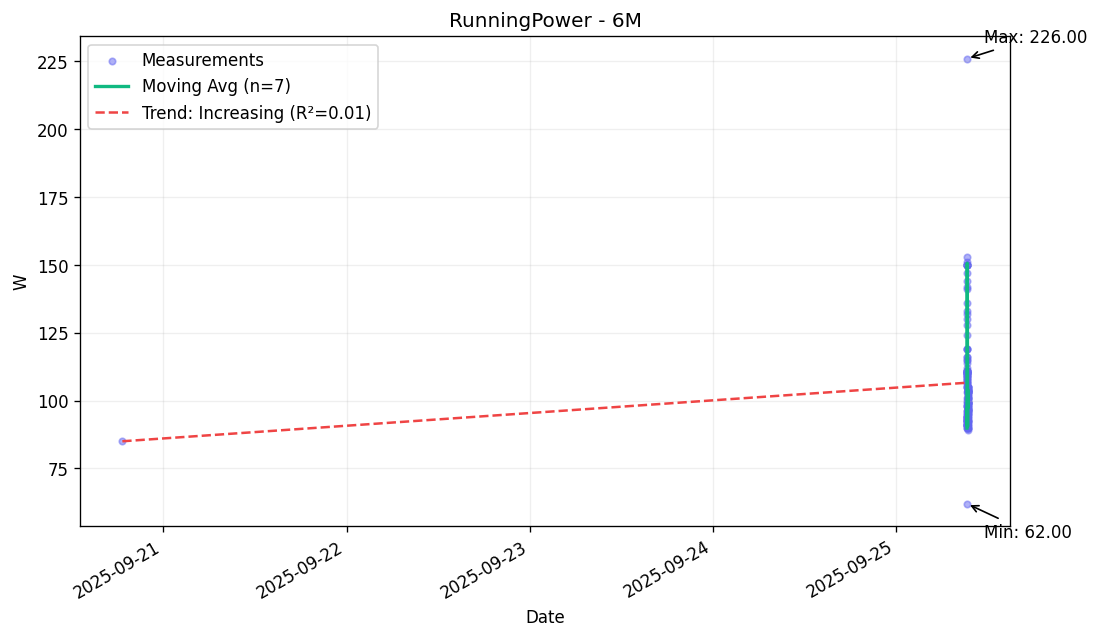
\includegraphics[width=0.95\textwidth]{plots_medical/Activity_and_Mobility/runningpower_6M.png}
\end{figure}
\begin{figure}[H]
\centering
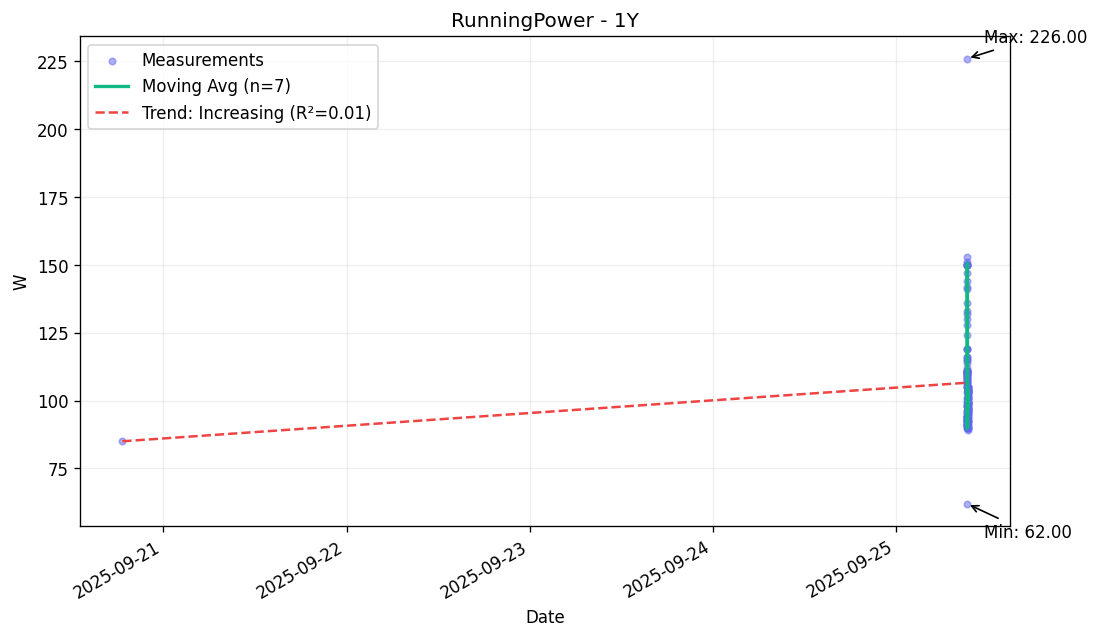
\includegraphics[width=0.95\textwidth]{plots_medical/Activity_and_Mobility/runningpower_1Y.png}
\end{figure}
\begin{figure}[H]
\centering
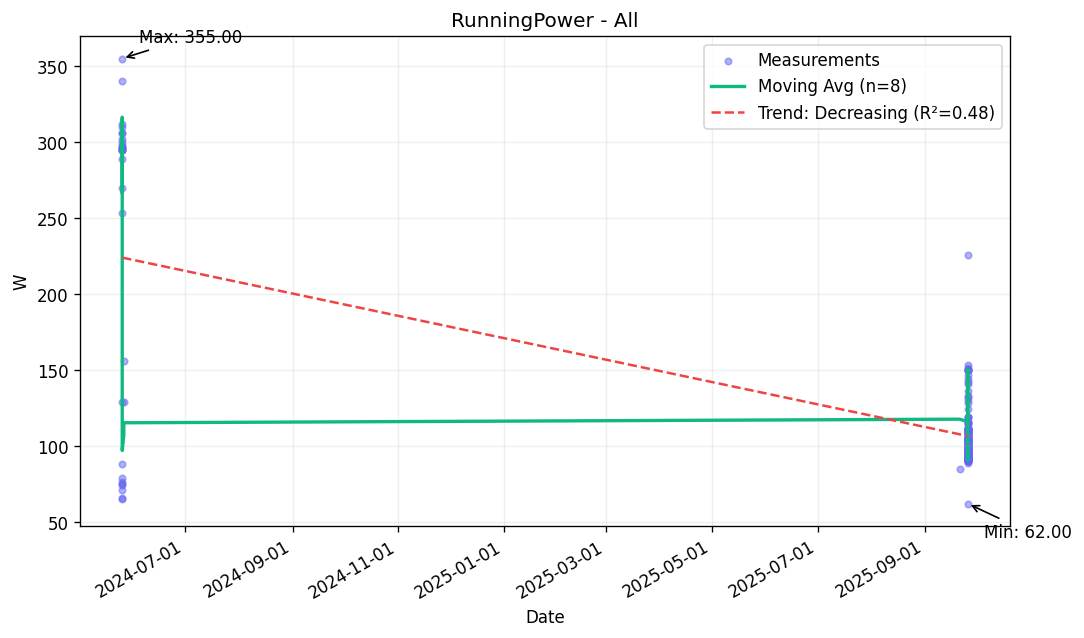
\includegraphics[width=0.95\textwidth]{plots_medical/Activity_and_Mobility/runningpower_All.png}
\end{figure}
\clearpage
\subsection{RunningSpeed}
\begin{table}[H]
\centering
\resizebox{\textwidth}{!}{
\begin{tabular}{|l|c|c|c|c|c|c|}
\hline
\textbf{Window} & \textbf{Min} & \textbf{Max} & \textbf{Avg} & \textbf{Start} & \textbf{End} & \textbf{Trend Slope} \\ \hline
1W & - & - & - & - & - & - \\ \hline
1M & - & - & - & - & - & - \\ \hline
3M & - & - & - & - & - & - \\ \hline
6M & - & - & - & - & - & - \\ \hline
1Y & - & - & - & - & - & - \\ \hline
All & 0.75 mi/hr & 8.98 mi/hr & 3.41 mi/hr & 2.62 & 2.61 & -0.00551 \\ \hline
\end{tabular}
}
\caption{Detailed Statistics for RunningSpeed}
\end{table}
\begin{figure}[H]
\centering
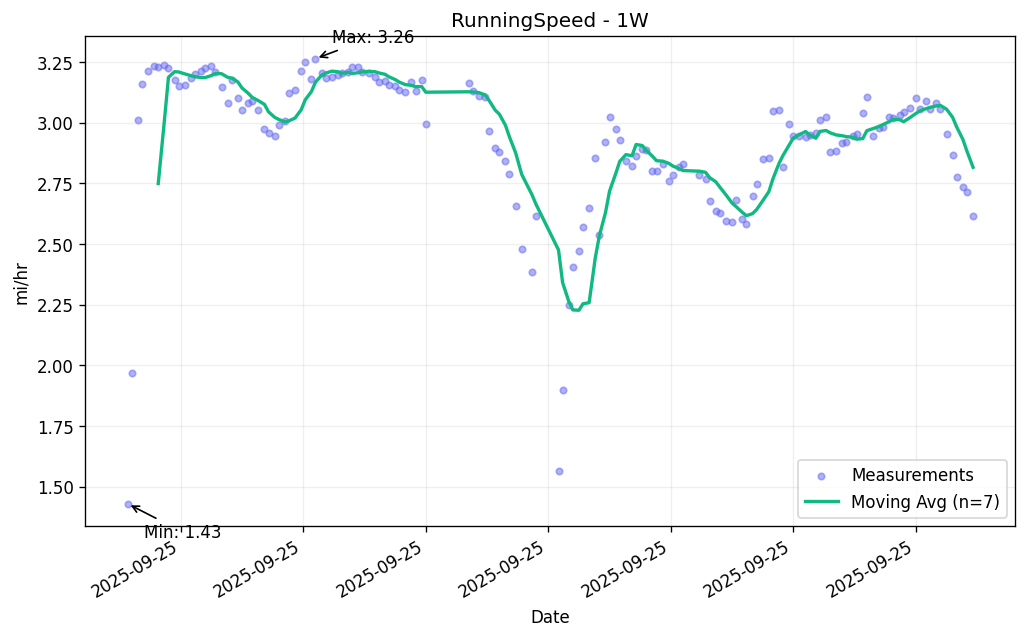
\includegraphics[width=0.95\textwidth]{plots_medical/Activity_and_Mobility/runningspeed_1W.png}
\end{figure}
\begin{figure}[H]
\centering
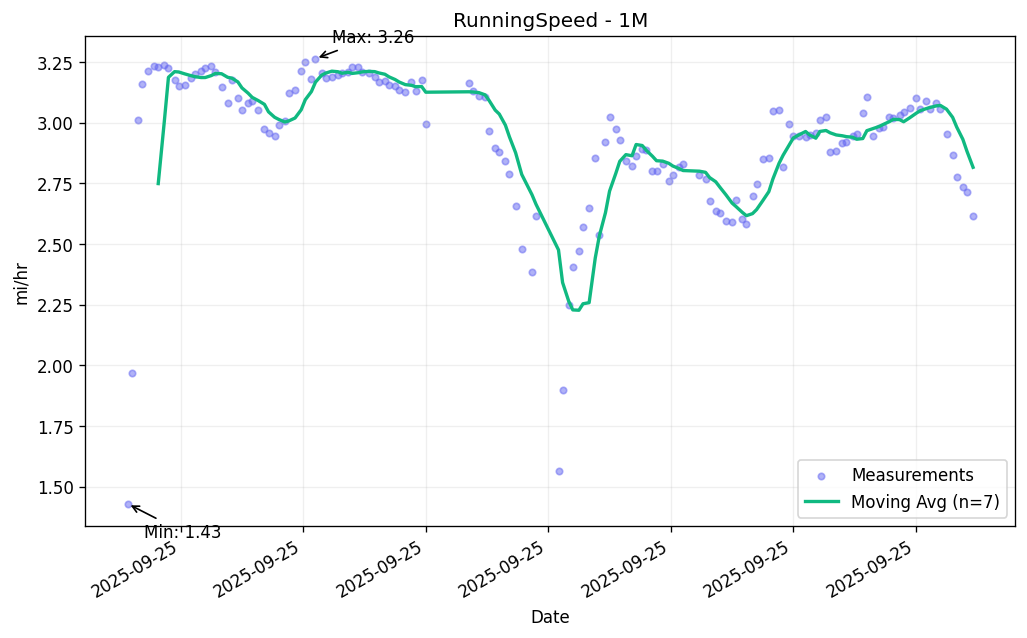
\includegraphics[width=0.95\textwidth]{plots_medical/Activity_and_Mobility/runningspeed_1M.png}
\end{figure}
\begin{figure}[H]
\centering
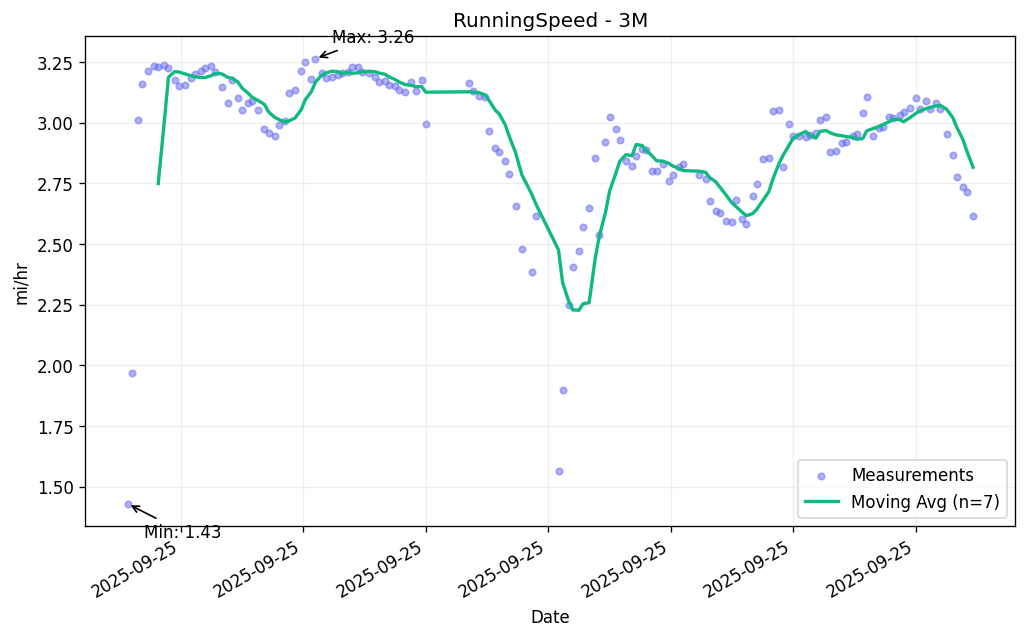
\includegraphics[width=0.95\textwidth]{plots_medical/Activity_and_Mobility/runningspeed_3M.png}
\end{figure}
\begin{figure}[H]
\centering
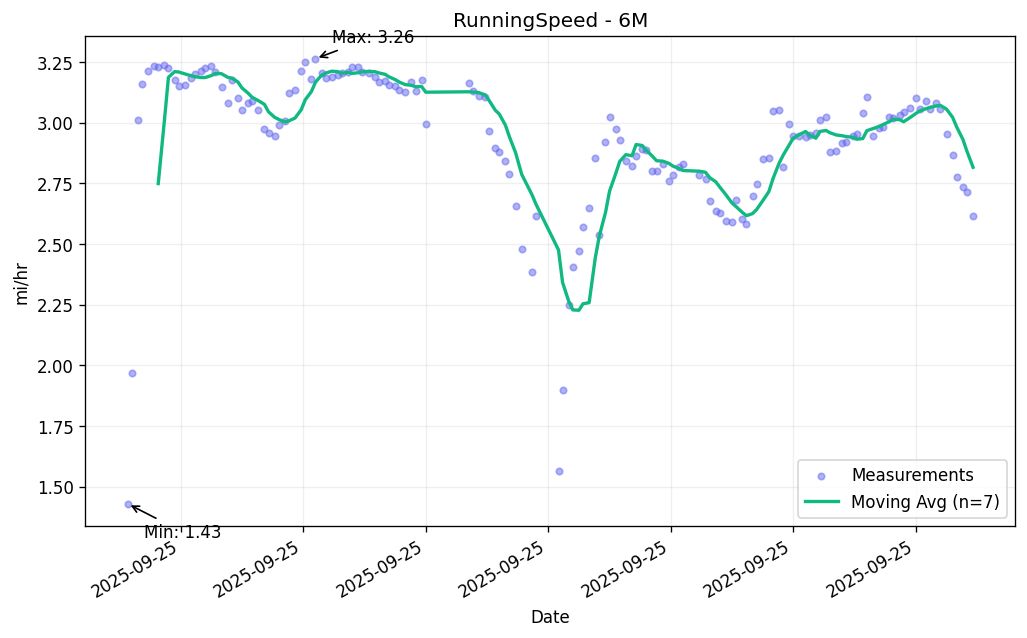
\includegraphics[width=0.95\textwidth]{plots_medical/Activity_and_Mobility/runningspeed_6M.png}
\end{figure}
\begin{figure}[H]
\centering
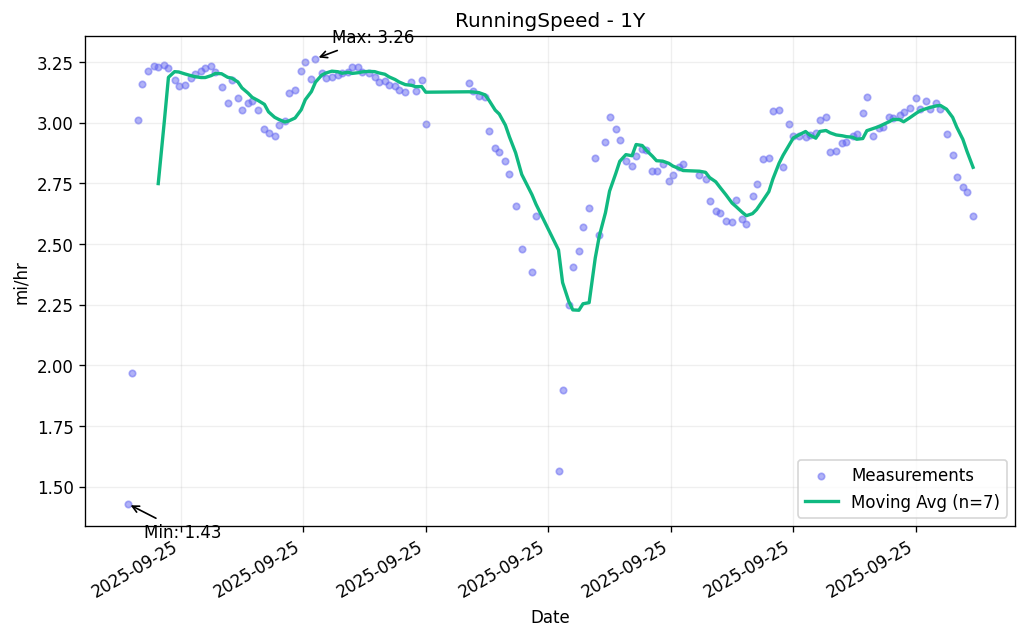
\includegraphics[width=0.95\textwidth]{plots_medical/Activity_and_Mobility/runningspeed_1Y.png}
\end{figure}
\begin{figure}[H]
\centering
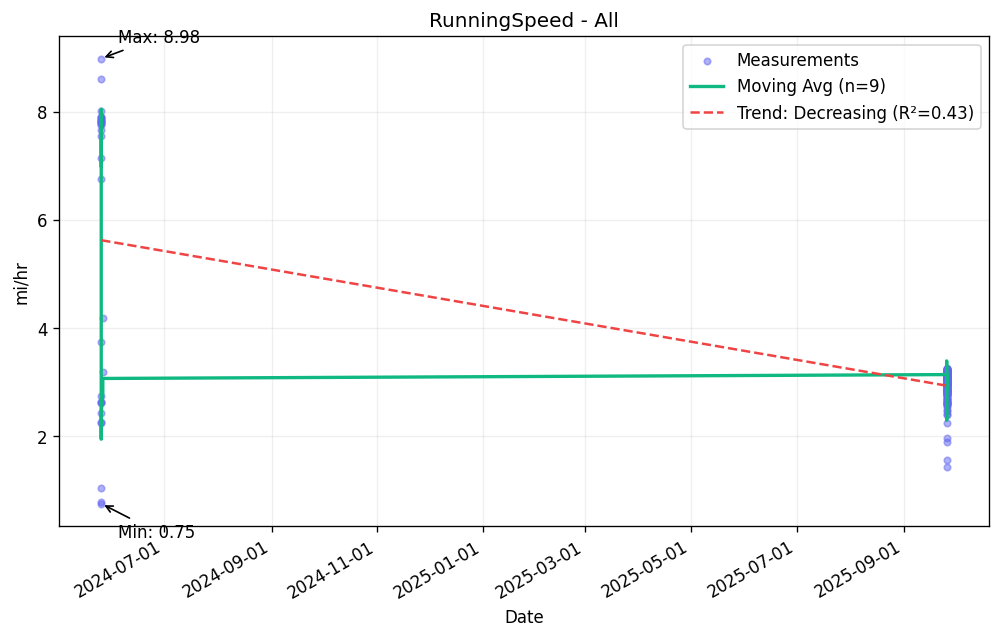
\includegraphics[width=0.95\textwidth]{plots_medical/Activity_and_Mobility/runningspeed_All.png}
\end{figure}
\clearpage
\subsection{RunningStrideLength}
\begin{table}[H]
\centering
\resizebox{\textwidth}{!}{
\begin{tabular}{|l|c|c|c|c|c|c|}
\hline
\textbf{Window} & \textbf{Min} & \textbf{Max} & \textbf{Avg} & \textbf{Start} & \textbf{End} & \textbf{Trend Slope} \\ \hline
1W & 1.28 m & 1.46 m & 1.39 m & 1.46 & 1.28 & -0.11941 \\ \hline
1M & 1.28 m & 1.46 m & 1.39 m & 1.46 & 1.28 & -0.11941 \\ \hline
3M & 1.28 m & 1.46 m & 1.39 m & 1.46 & 1.28 & -0.11941 \\ \hline
6M & 1.28 m & 1.46 m & 1.39 m & 1.46 & 1.28 & -0.11941 \\ \hline
1Y & 1.28 m & 1.46 m & 1.39 m & 1.46 & 1.28 & -0.11941 \\ \hline
All & 1.28 m & 1.46 m & 1.39 m & 1.46 & 1.28 & -0.11941 \\ \hline
\end{tabular}
}
\caption{Detailed Statistics for RunningStrideLength}
\end{table}
\begin{figure}[H]
\centering
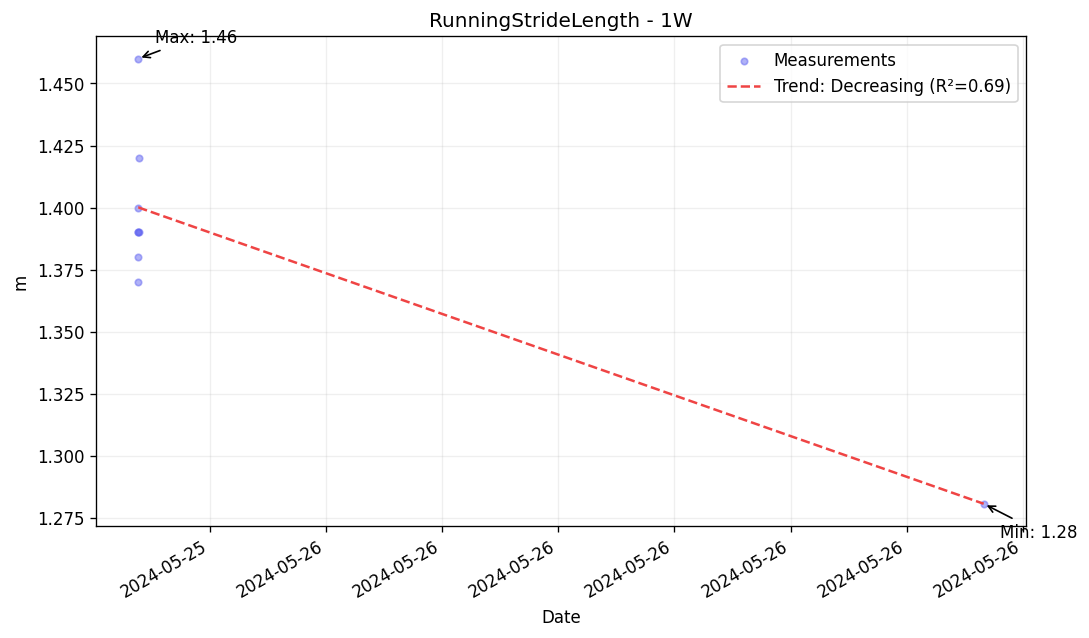
\includegraphics[width=0.95\textwidth]{plots_medical/Activity_and_Mobility/runningstridelength_1W.png}
\end{figure}
\begin{figure}[H]
\centering
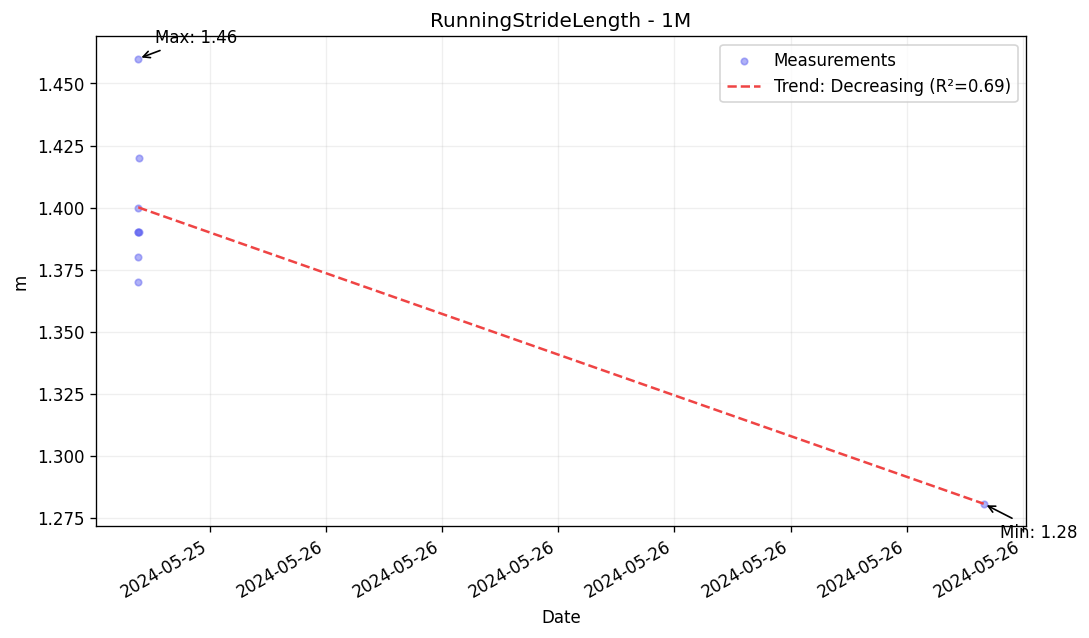
\includegraphics[width=0.95\textwidth]{plots_medical/Activity_and_Mobility/runningstridelength_1M.png}
\end{figure}
\begin{figure}[H]
\centering
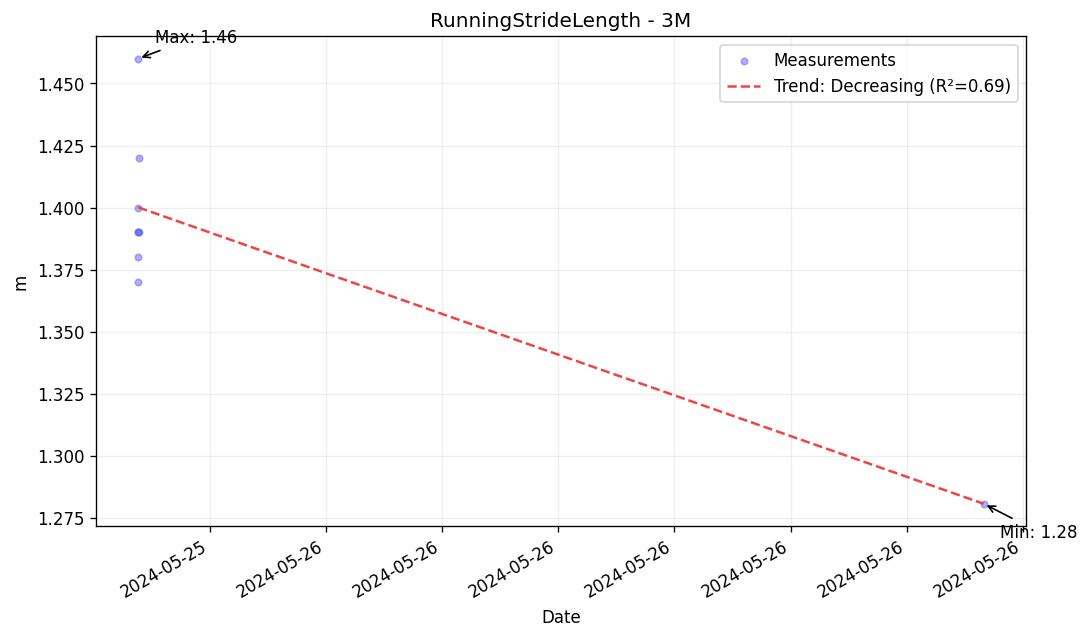
\includegraphics[width=0.95\textwidth]{plots_medical/Activity_and_Mobility/runningstridelength_3M.png}
\end{figure}
\begin{figure}[H]
\centering
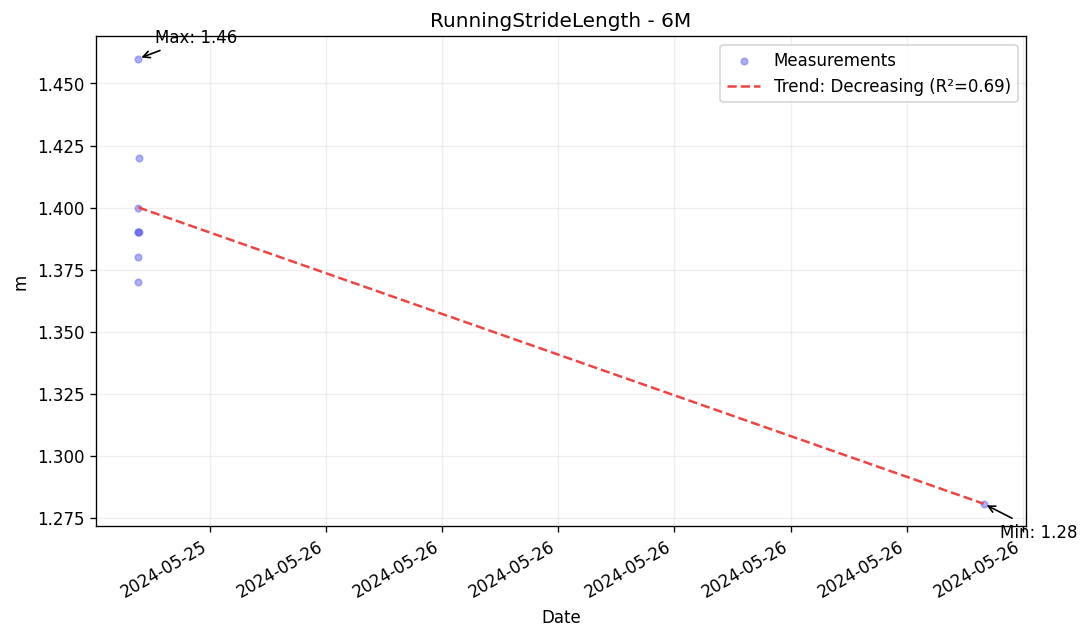
\includegraphics[width=0.95\textwidth]{plots_medical/Activity_and_Mobility/runningstridelength_6M.png}
\end{figure}
\begin{figure}[H]
\centering
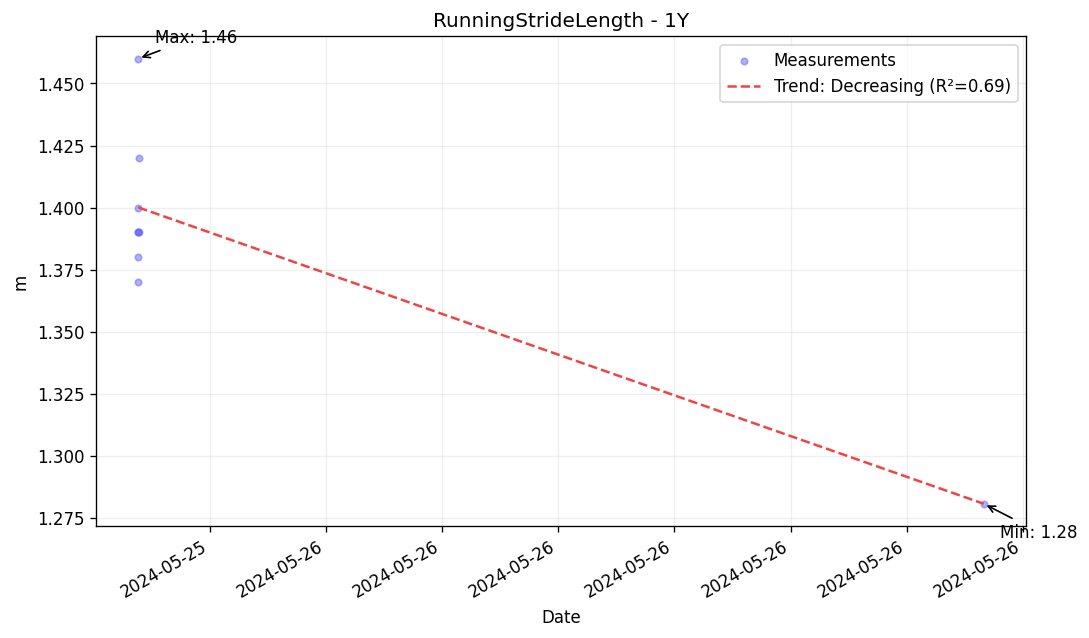
\includegraphics[width=0.95\textwidth]{plots_medical/Activity_and_Mobility/runningstridelength_1Y.png}
\end{figure}
\begin{figure}[H]
\centering
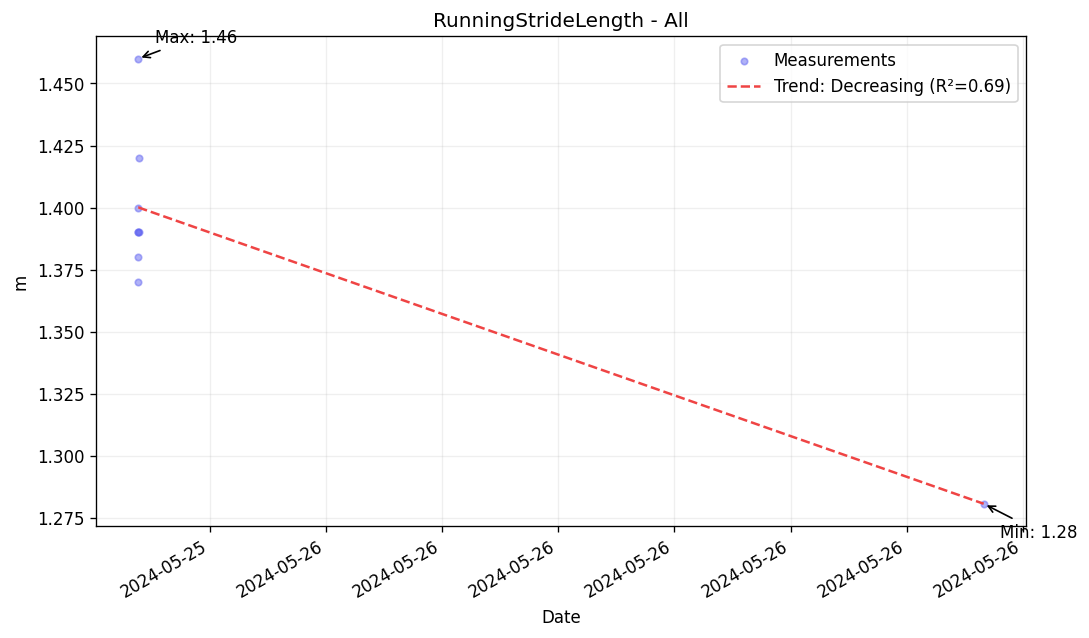
\includegraphics[width=0.95\textwidth]{plots_medical/Activity_and_Mobility/runningstridelength_All.png}
\end{figure}
\clearpage
\subsection{RunningVerticalOscillation}
\begin{table}[H]
\centering
\resizebox{\textwidth}{!}{
\begin{tabular}{|l|c|c|c|c|c|c|}
\hline
\textbf{Window} & \textbf{Min} & \textbf{Max} & \textbf{Avg} & \textbf{Start} & \textbf{End} & \textbf{Trend Slope} \\ \hline
1W & 9.70 cm & 10.81 cm & 10.09 cm & 9.70 & 10.81 & 0.79679 \\ \hline
1M & 9.70 cm & 10.81 cm & 10.09 cm & 9.70 & 10.81 & 0.79679 \\ \hline
3M & 9.70 cm & 10.81 cm & 10.09 cm & 9.70 & 10.81 & 0.79679 \\ \hline
6M & 9.70 cm & 10.81 cm & 10.09 cm & 9.70 & 10.81 & 0.79679 \\ \hline
1Y & 9.70 cm & 10.81 cm & 10.09 cm & 9.70 & 10.81 & 0.79679 \\ \hline
All & 9.70 cm & 10.81 cm & 10.09 cm & 9.70 & 10.81 & 0.79679 \\ \hline
\end{tabular}
}
\caption{Detailed Statistics for RunningVerticalOscillation}
\end{table}
\begin{figure}[H]
\centering
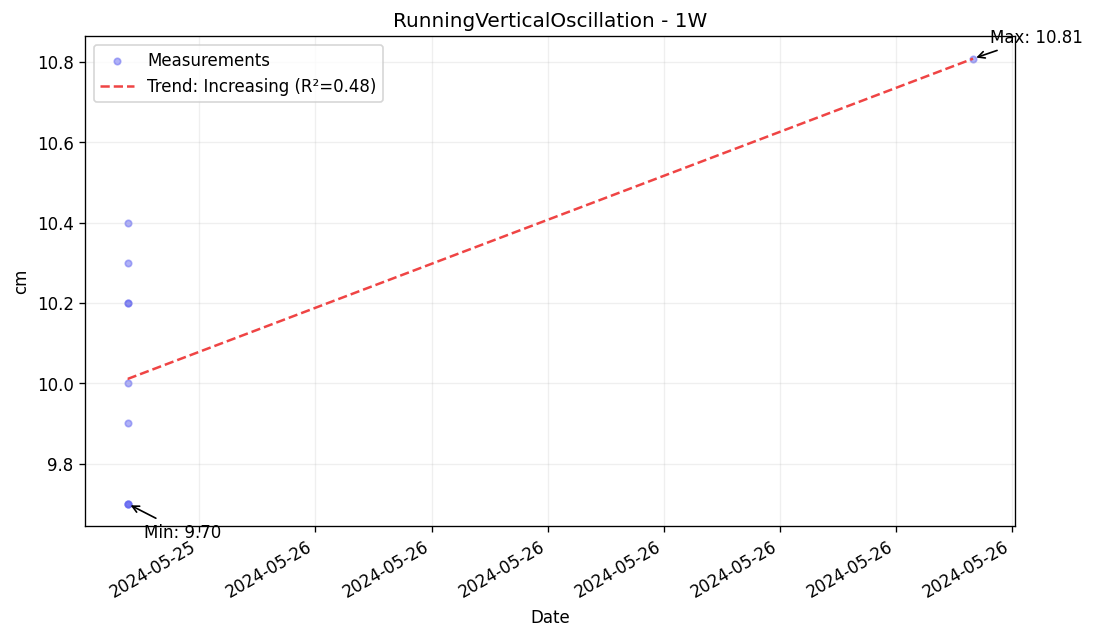
\includegraphics[width=0.95\textwidth]{plots_medical/Activity_and_Mobility/runningverticaloscillation_1W.png}
\end{figure}
\begin{figure}[H]
\centering
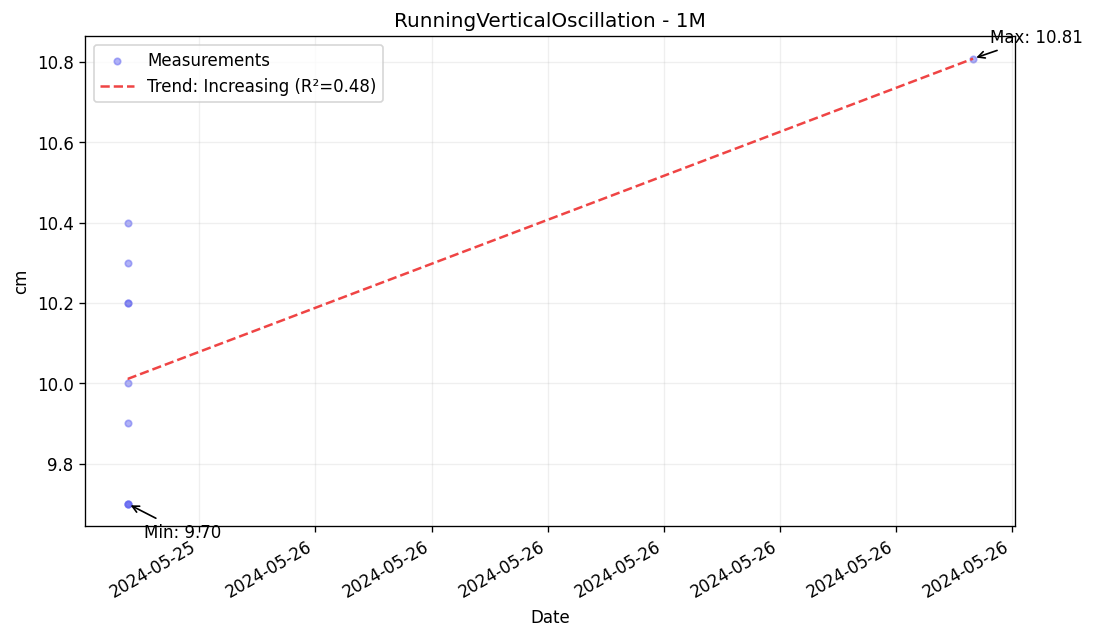
\includegraphics[width=0.95\textwidth]{plots_medical/Activity_and_Mobility/runningverticaloscillation_1M.png}
\end{figure}
\begin{figure}[H]
\centering
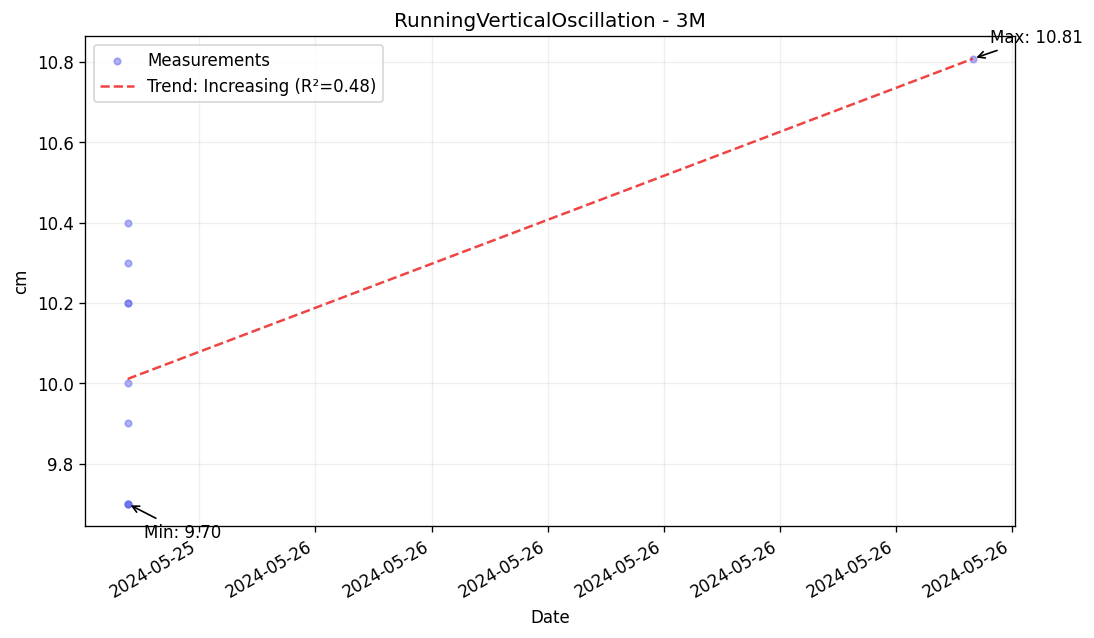
\includegraphics[width=0.95\textwidth]{plots_medical/Activity_and_Mobility/runningverticaloscillation_3M.png}
\end{figure}
\begin{figure}[H]
\centering
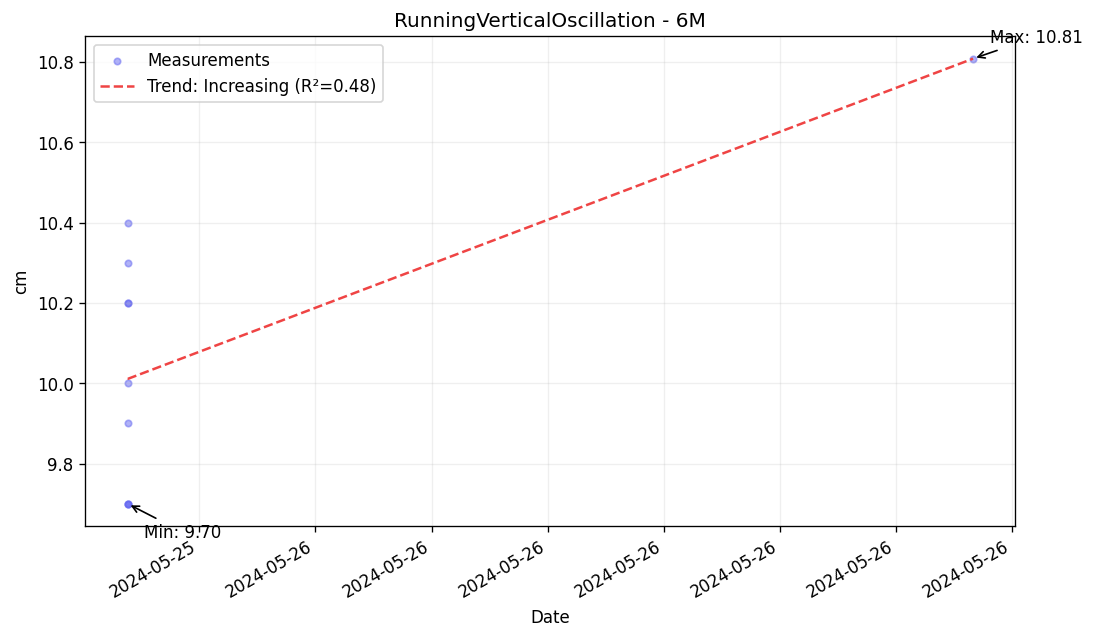
\includegraphics[width=0.95\textwidth]{plots_medical/Activity_and_Mobility/runningverticaloscillation_6M.png}
\end{figure}
\begin{figure}[H]
\centering
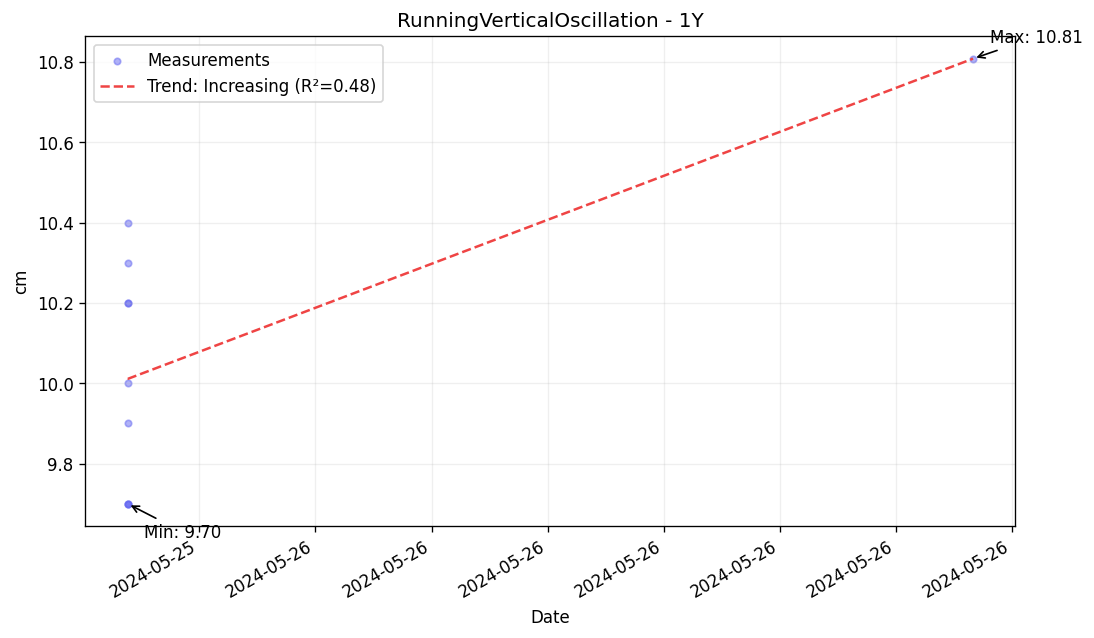
\includegraphics[width=0.95\textwidth]{plots_medical/Activity_and_Mobility/runningverticaloscillation_1Y.png}
\end{figure}
\begin{figure}[H]
\centering
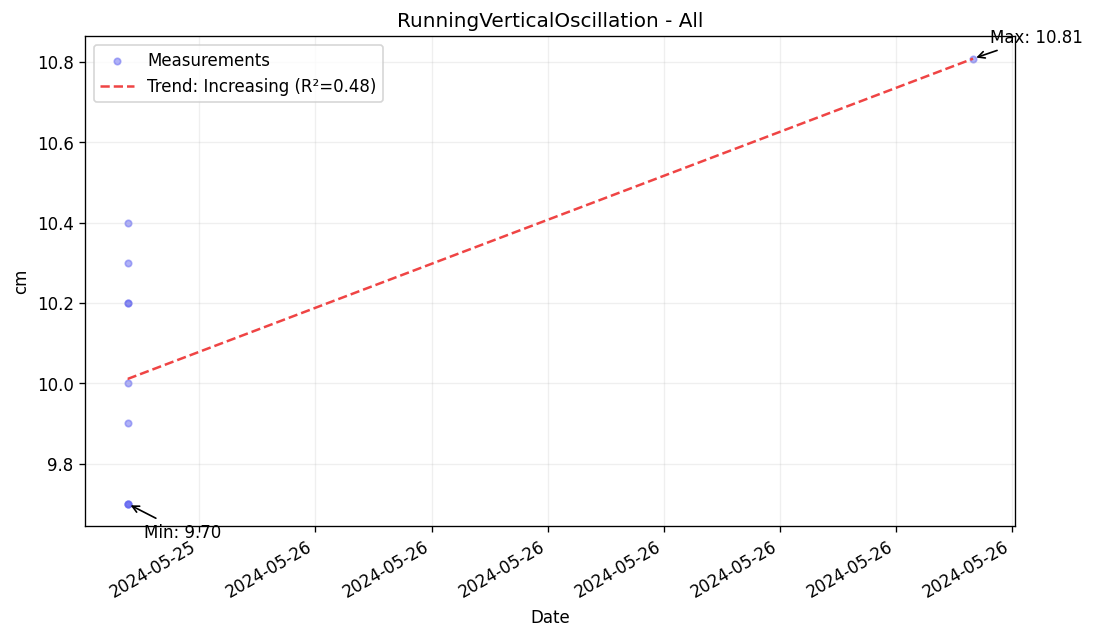
\includegraphics[width=0.95\textwidth]{plots_medical/Activity_and_Mobility/runningverticaloscillation_All.png}
\end{figure}
\clearpage
\subsection{SixMinuteWalkTestDistance}
\begin{table}[H]
\centering
\resizebox{\textwidth}{!}{
\begin{tabular}{|l|c|c|c|c|c|c|}
\hline
\textbf{Window} & \textbf{Min} & \textbf{Max} & \textbf{Avg} & \textbf{Start} & \textbf{End} & \textbf{Trend Slope} \\ \hline
1W & - & - & - & - & - & - \\ \hline
1M & 480.00 m & 500.00 m & 487.40 m & 500.00 & 480.00 & -0.58665 \\ \hline
3M & 480.00 m & 500.00 m & 495.15 m & 500.00 & 480.00 & -0.22617 \\ \hline
6M & 448.00 m & 500.00 m & 486.12 m & 448.00 & 480.00 & 0.17491 \\ \hline
1Y & 448.00 m & 500.00 m & 489.25 m & 500.00 & 480.00 & -0.01125 \\ \hline
All & 437.00 m & 500.00 m & 492.62 m & 500.00 & 480.00 & -0.01552 \\ \hline
\end{tabular}
}
\caption{Detailed Statistics for SixMinuteWalkTestDistance}
\end{table}
\begin{figure}[H]
\centering
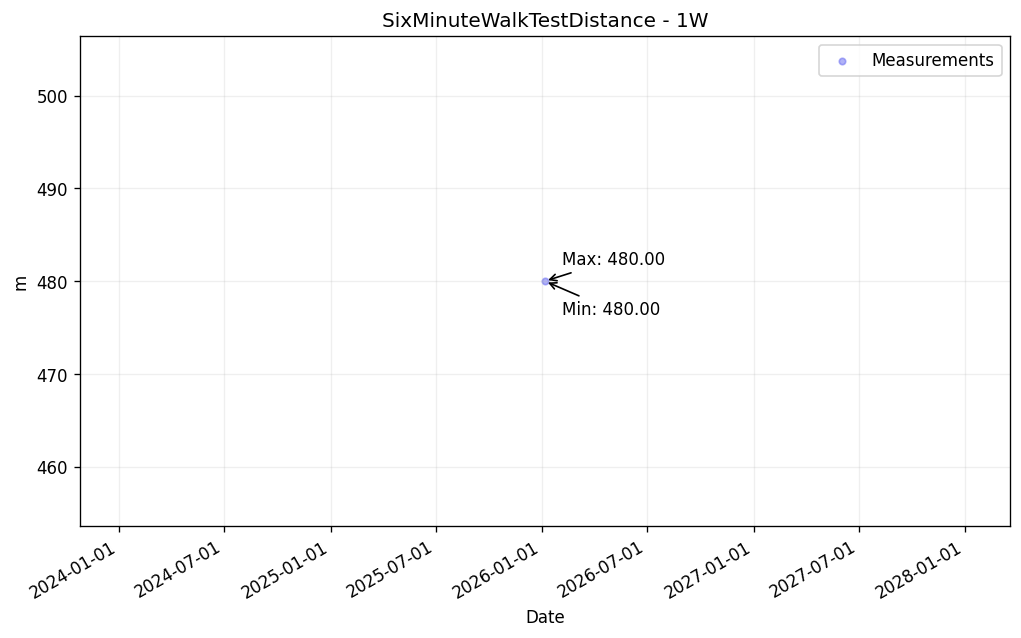
\includegraphics[width=0.95\textwidth]{plots_medical/Activity_and_Mobility/sixminutewalktestdistance_1W.png}
\end{figure}
\begin{figure}[H]
\centering
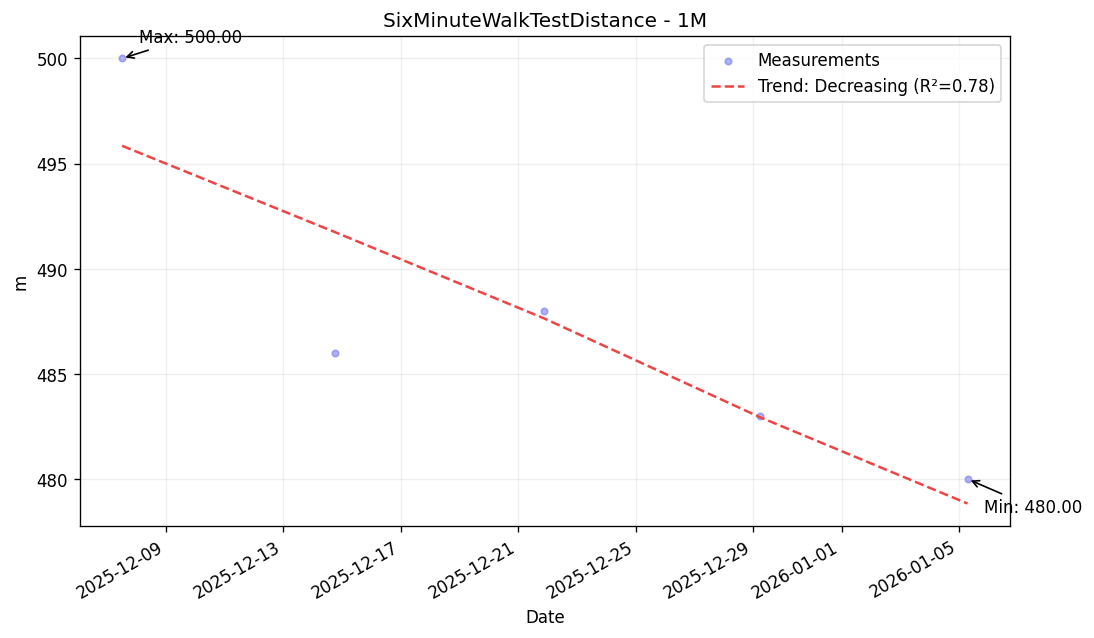
\includegraphics[width=0.95\textwidth]{plots_medical/Activity_and_Mobility/sixminutewalktestdistance_1M.png}
\end{figure}
\begin{figure}[H]
\centering
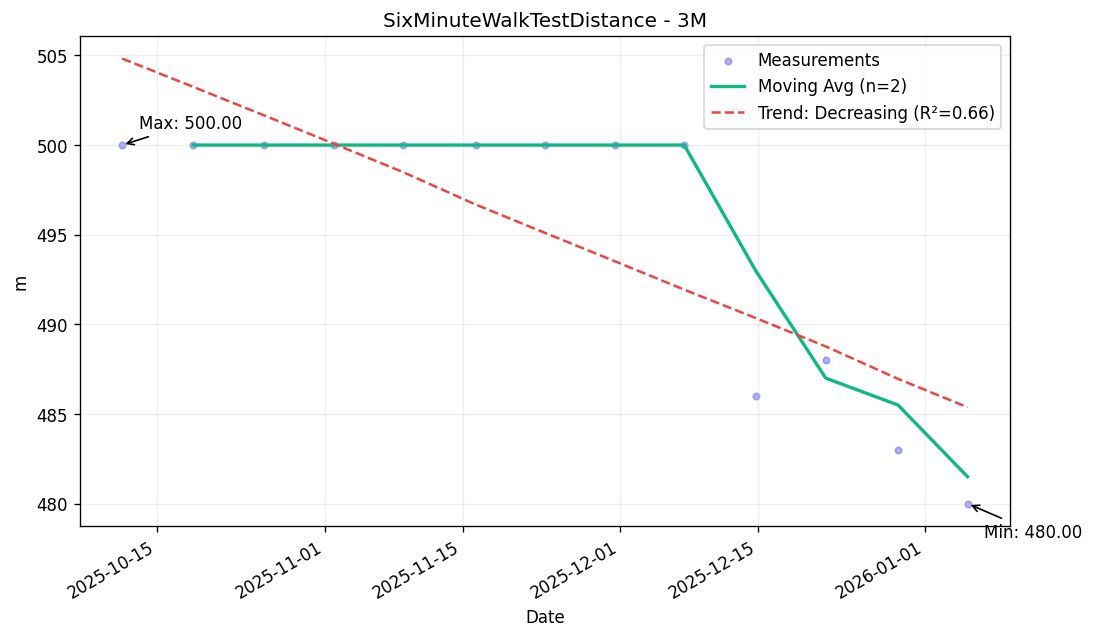
\includegraphics[width=0.95\textwidth]{plots_medical/Activity_and_Mobility/sixminutewalktestdistance_3M.png}
\end{figure}
\begin{figure}[H]
\centering
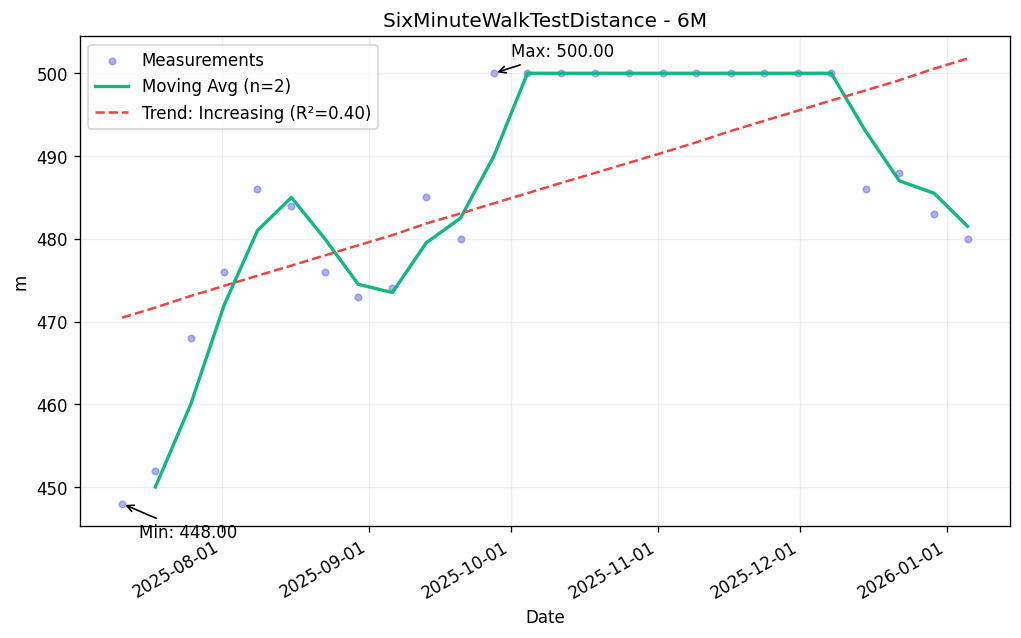
\includegraphics[width=0.95\textwidth]{plots_medical/Activity_and_Mobility/sixminutewalktestdistance_6M.png}
\end{figure}
\begin{figure}[H]
\centering
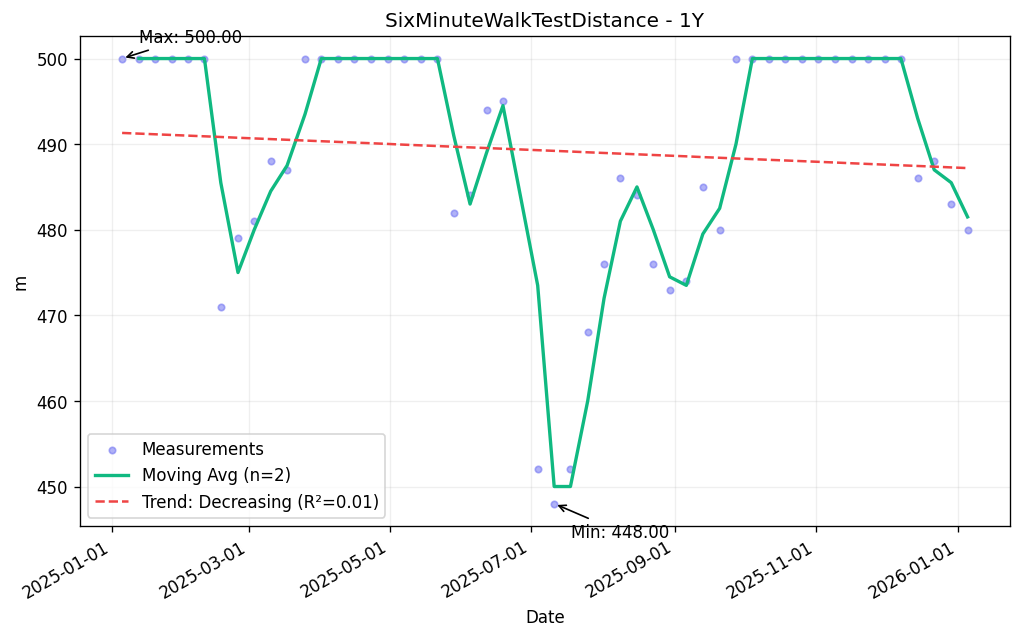
\includegraphics[width=0.95\textwidth]{plots_medical/Activity_and_Mobility/sixminutewalktestdistance_1Y.png}
\end{figure}
\begin{figure}[H]
\centering
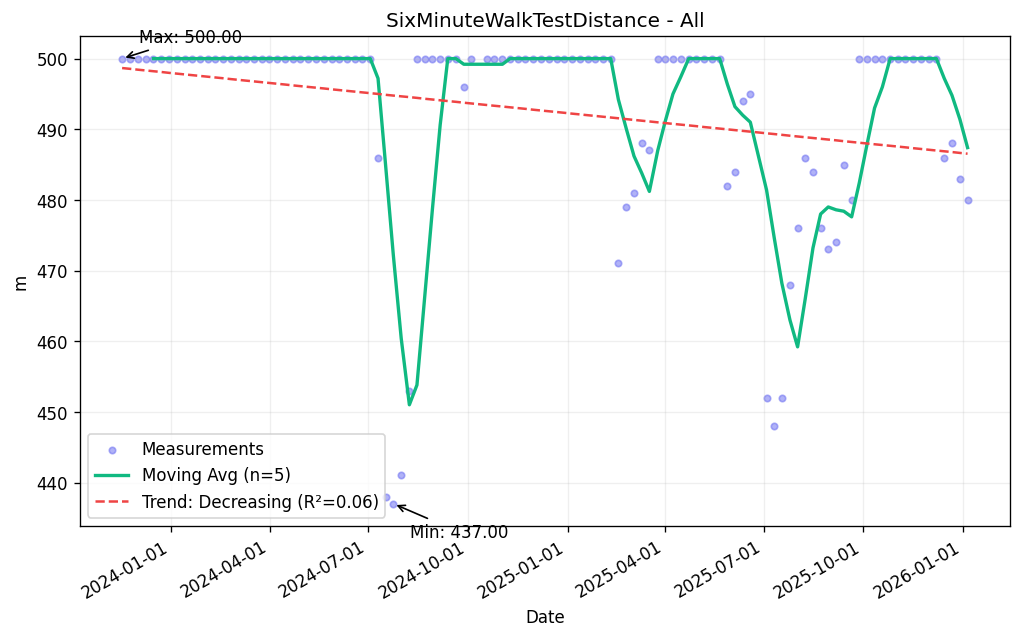
\includegraphics[width=0.95\textwidth]{plots_medical/Activity_and_Mobility/sixminutewalktestdistance_All.png}
\end{figure}
\clearpage
\subsection{StairAscentSpeed}
\begin{table}[H]
\centering
\resizebox{\textwidth}{!}{
\begin{tabular}{|l|c|c|c|c|c|c|}
\hline
\textbf{Window} & \textbf{Min} & \textbf{Max} & \textbf{Avg} & \textbf{Start} & \textbf{End} & \textbf{Trend Slope} \\ \hline
1W & 0.67 ft/s & 1.86 ft/s & 0.99 ft/s & 1.86 & 0.95 & 0.00782 \\ \hline
1M & 0.67 ft/s & 1.86 ft/s & 0.95 ft/s & 0.85 & 0.95 & 0.00377 \\ \hline
3M & 0.67 ft/s & 2.20 ft/s & 0.96 ft/s & 1.01 & 0.95 & -0.00006 \\ \hline
6M & 0.66 ft/s & 2.28 ft/s & 0.94 ft/s & 0.79 & 0.95 & 0.00044 \\ \hline
1Y & 0.66 ft/s & 2.28 ft/s & 0.93 ft/s & 0.94 & 0.95 & 0.00018 \\ \hline
All & 0.66 ft/s & 3.54 ft/s & 0.95 ft/s & 0.97 & 0.95 & -0.00006 \\ \hline
\end{tabular}
}
\caption{Detailed Statistics for StairAscentSpeed}
\end{table}
\begin{figure}[H]
\centering
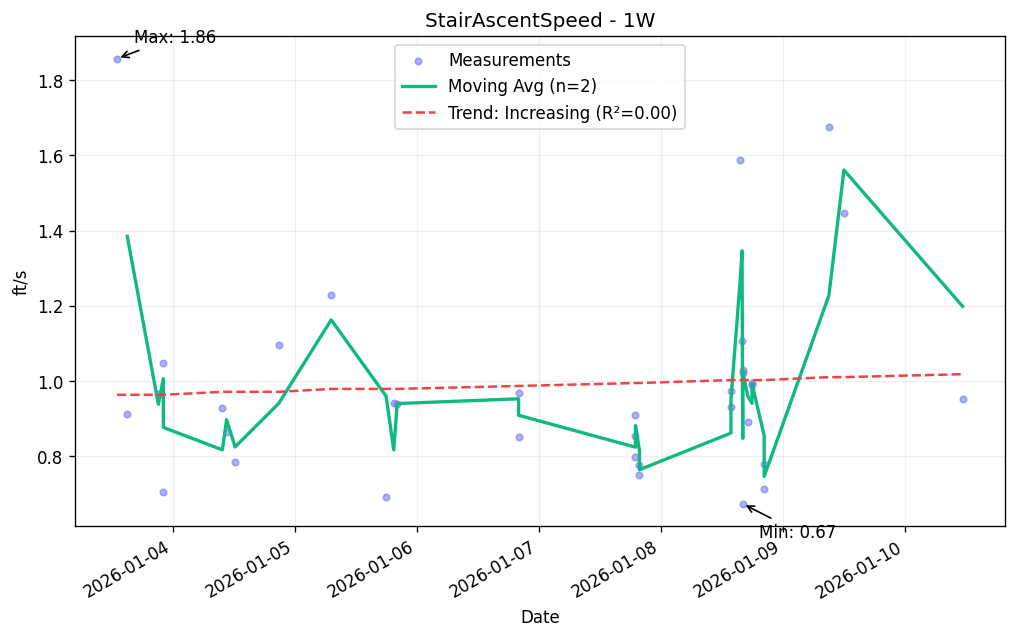
\includegraphics[width=0.95\textwidth]{plots_medical/Activity_and_Mobility/stairascentspeed_1W.png}
\end{figure}
\begin{figure}[H]
\centering
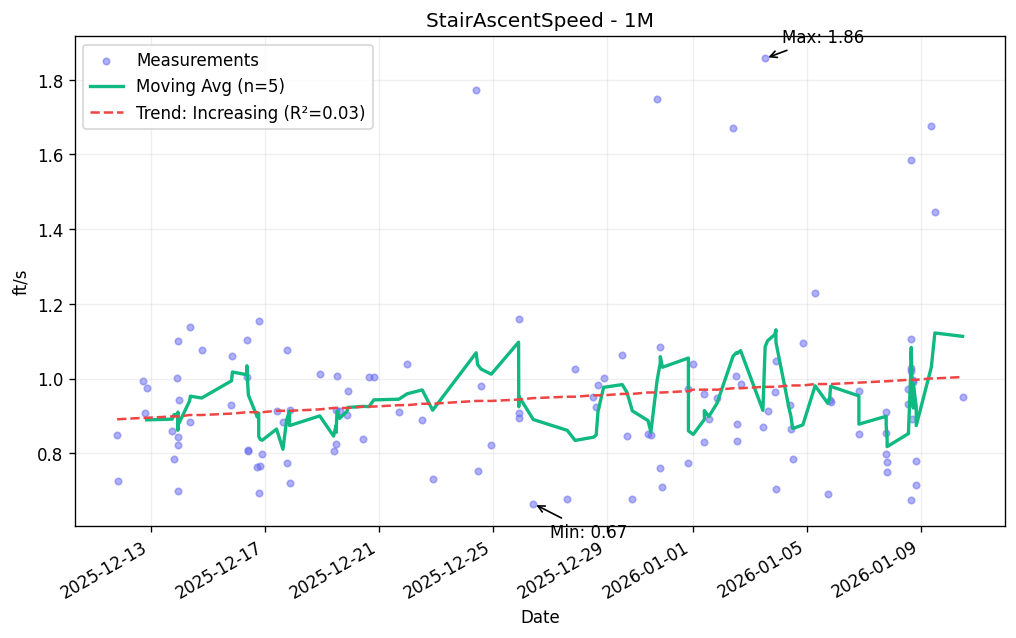
\includegraphics[width=0.95\textwidth]{plots_medical/Activity_and_Mobility/stairascentspeed_1M.png}
\end{figure}
\begin{figure}[H]
\centering
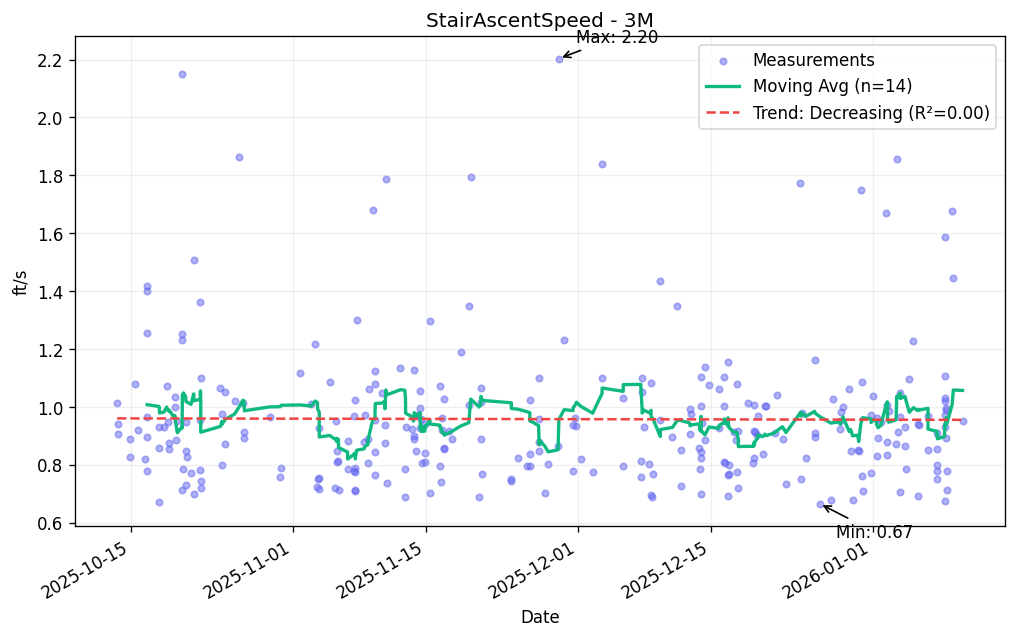
\includegraphics[width=0.95\textwidth]{plots_medical/Activity_and_Mobility/stairascentspeed_3M.png}
\end{figure}
\begin{figure}[H]
\centering
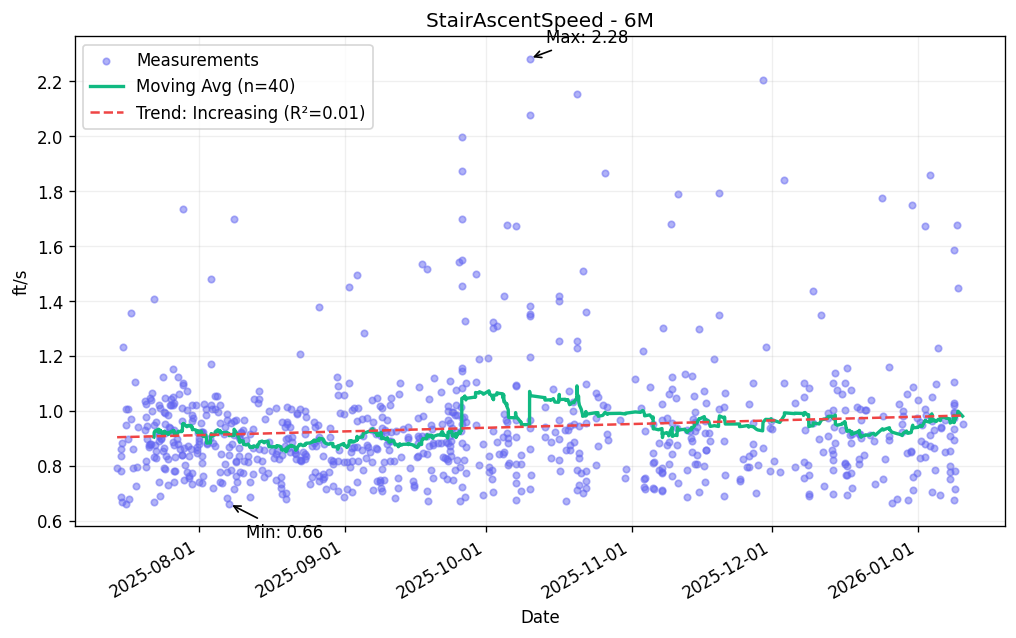
\includegraphics[width=0.95\textwidth]{plots_medical/Activity_and_Mobility/stairascentspeed_6M.png}
\end{figure}
\begin{figure}[H]
\centering
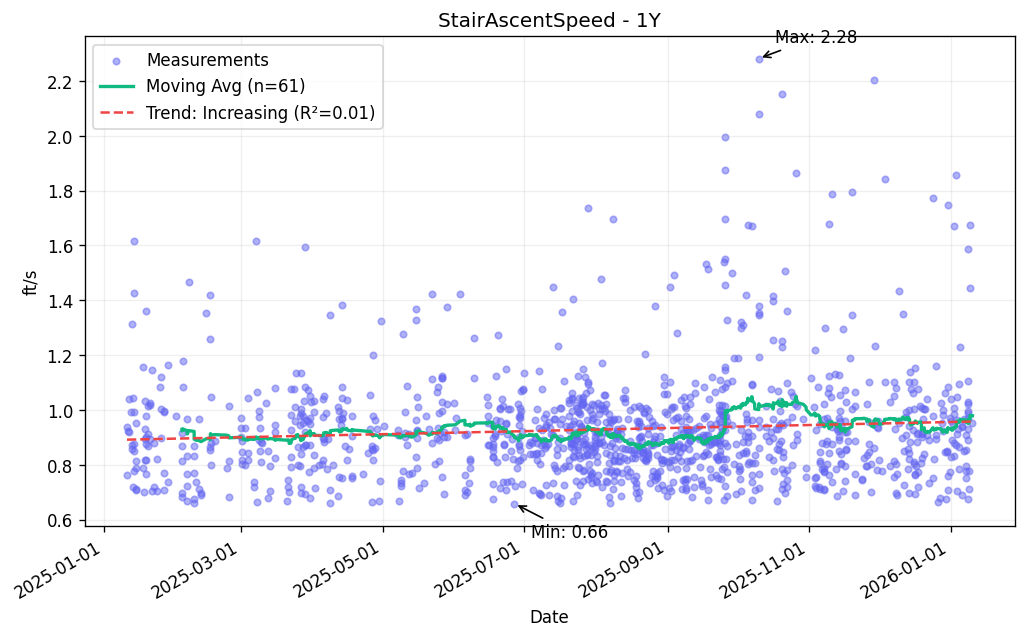
\includegraphics[width=0.95\textwidth]{plots_medical/Activity_and_Mobility/stairascentspeed_1Y.png}
\end{figure}
\begin{figure}[H]
\centering
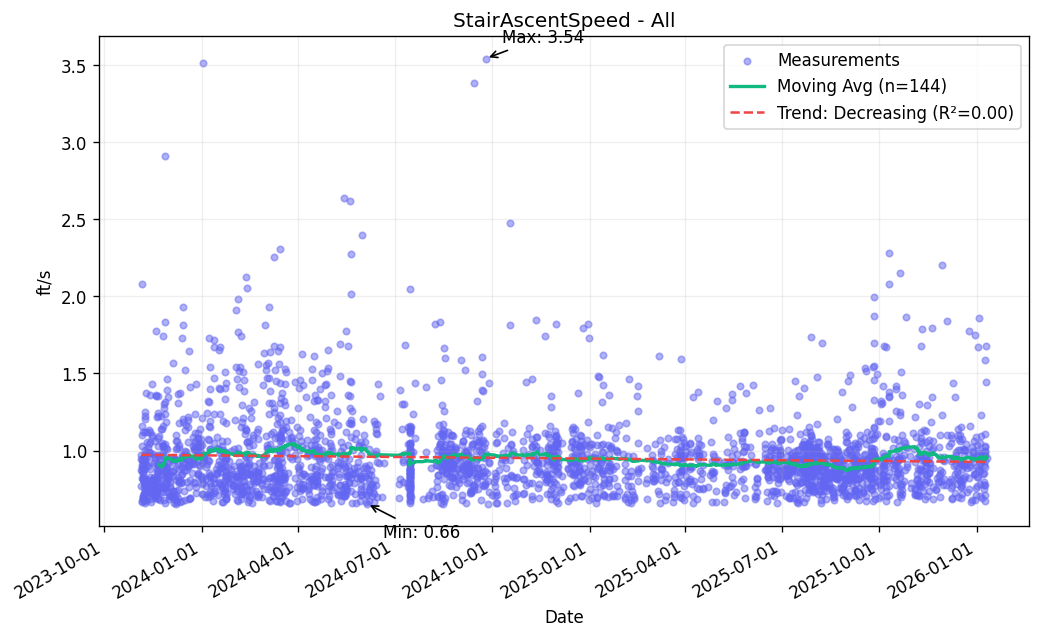
\includegraphics[width=0.95\textwidth]{plots_medical/Activity_and_Mobility/stairascentspeed_All.png}
\end{figure}
\clearpage
\subsection{StairDescentSpeed}
\begin{table}[H]
\centering
\resizebox{\textwidth}{!}{
\begin{tabular}{|l|c|c|c|c|c|c|}
\hline
\textbf{Window} & \textbf{Min} & \textbf{Max} & \textbf{Avg} & \textbf{Start} & \textbf{End} & \textbf{Trend Slope} \\ \hline
1W & 0.67 ft/s & 2.20 ft/s & 1.21 ft/s & 1.40 & 1.14 & -0.10576 \\ \hline
1M & 0.66 ft/s & 2.20 ft/s & 1.34 ft/s & 1.34 & 1.14 & -0.00619 \\ \hline
3M & 0.66 ft/s & 2.20 ft/s & 1.27 ft/s & 0.80 & 1.14 & 0.00190 \\ \hline
6M & 0.66 ft/s & 2.87 ft/s & 1.29 ft/s & 1.20 & 1.14 & -0.00058 \\ \hline
1Y & 0.66 ft/s & 2.87 ft/s & 1.25 ft/s & 1.22 & 1.14 & 0.00024 \\ \hline
All & 0.66 ft/s & 3.14 ft/s & 1.21 ft/s & 1.73 & 1.14 & 0.00020 \\ \hline
\end{tabular}
}
\caption{Detailed Statistics for StairDescentSpeed}
\end{table}
\begin{figure}[H]
\centering
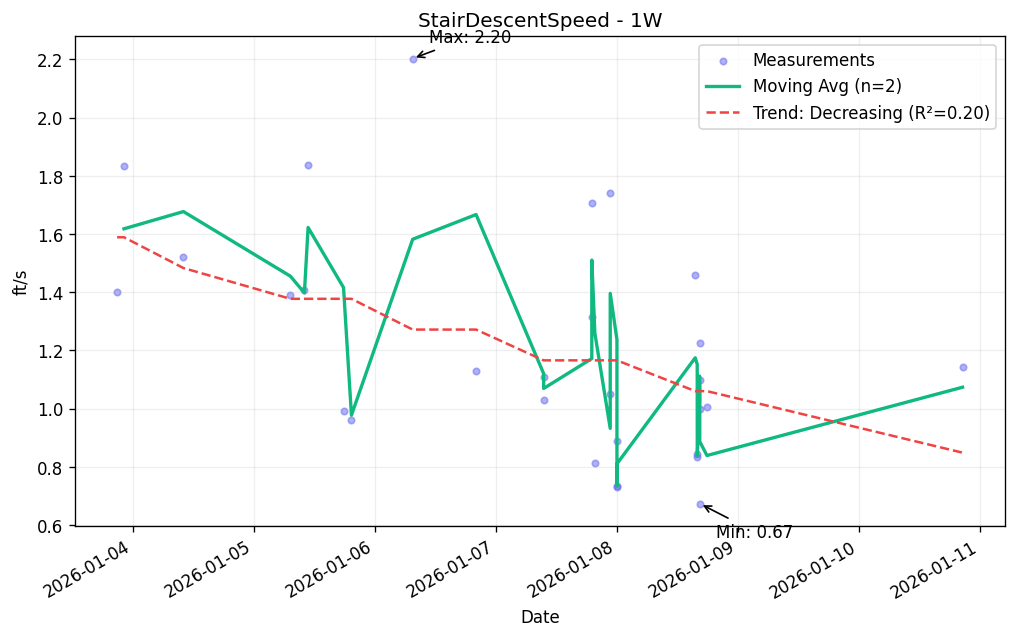
\includegraphics[width=0.95\textwidth]{plots_medical/Activity_and_Mobility/stairdescentspeed_1W.png}
\end{figure}
\begin{figure}[H]
\centering
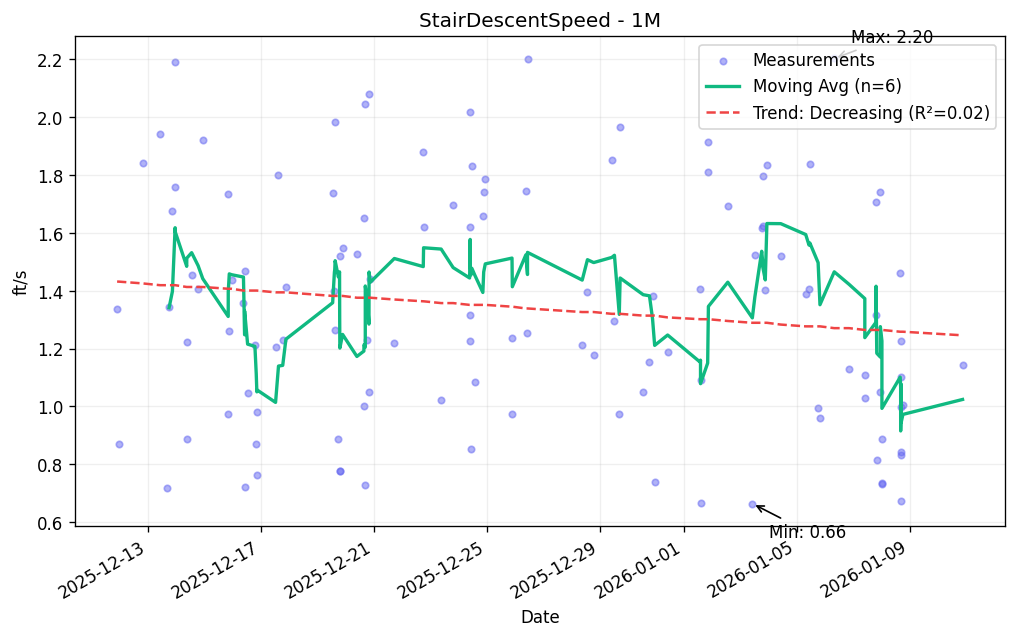
\includegraphics[width=0.95\textwidth]{plots_medical/Activity_and_Mobility/stairdescentspeed_1M.png}
\end{figure}
\begin{figure}[H]
\centering
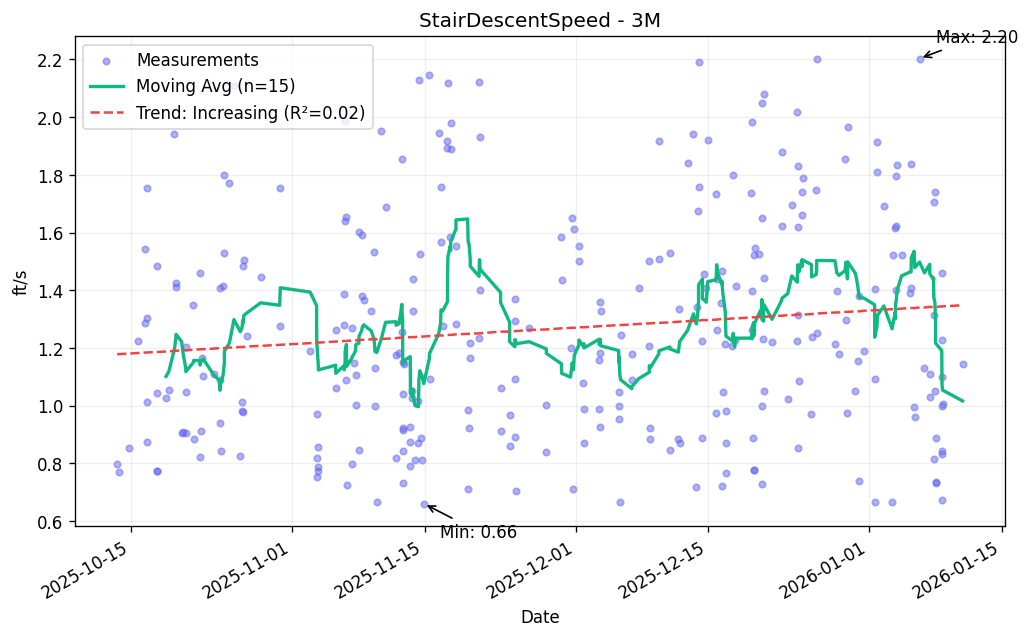
\includegraphics[width=0.95\textwidth]{plots_medical/Activity_and_Mobility/stairdescentspeed_3M.png}
\end{figure}
\begin{figure}[H]
\centering
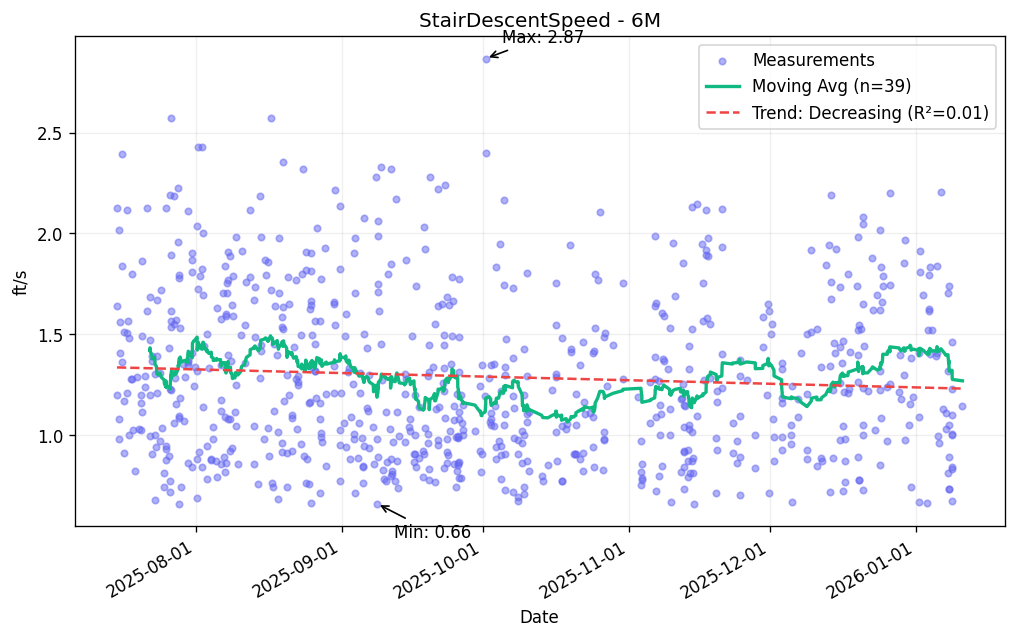
\includegraphics[width=0.95\textwidth]{plots_medical/Activity_and_Mobility/stairdescentspeed_6M.png}
\end{figure}
\begin{figure}[H]
\centering
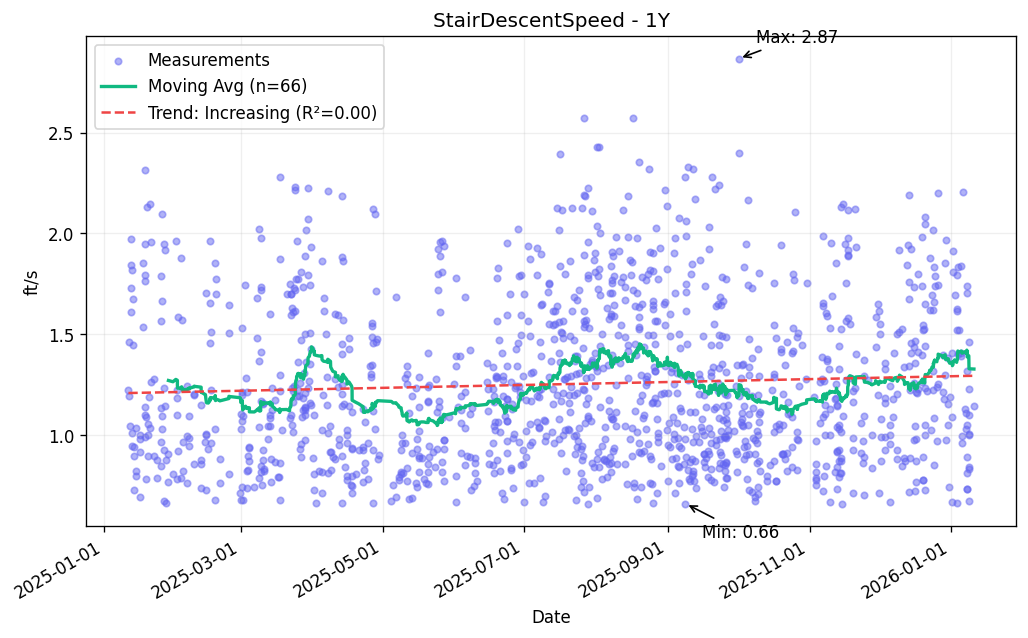
\includegraphics[width=0.95\textwidth]{plots_medical/Activity_and_Mobility/stairdescentspeed_1Y.png}
\end{figure}
\begin{figure}[H]
\centering
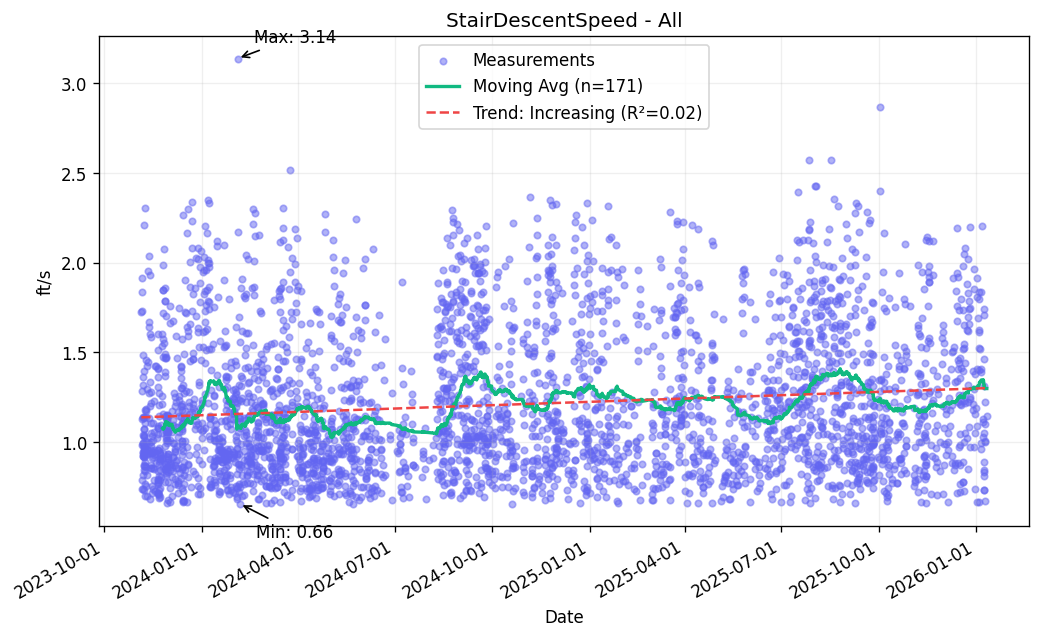
\includegraphics[width=0.95\textwidth]{plots_medical/Activity_and_Mobility/stairdescentspeed_All.png}
\end{figure}
\clearpage
\subsection{StepCount}
\begin{table}[H]
\centering
\resizebox{\textwidth}{!}{
\begin{tabular}{|l|c|c|c|c|c|c|}
\hline
\textbf{Window} & \textbf{Min} & \textbf{Max} & \textbf{Avg} & \textbf{Start} & \textbf{End} & \textbf{Trend Slope} \\ \hline
1W & 1.00 count & 1070.00 count & 148.94 count & 16.00 & 35.00 & 5.83689 \\ \hline
1M & 1.00 count & 1070.00 count & 111.87 count & 68.00 & 35.00 & 3.19872 \\ \hline
3M & 1.00 count & 1073.00 count & 147.74 count & 28.00 & 35.00 & -0.70099 \\ \hline
6M & 1.00 count & 1073.00 count & 136.39 count & 12.00 & 35.00 & 0.21094 \\ \hline
1Y & 1.00 count & 1124.00 count & 152.45 count & 14.00 & 35.00 & -0.12383 \\ \hline
All & 1.00 count & 1237.00 count & 169.79 count & 63.00 & 35.00 & 0.00889 \\ \hline
\end{tabular}
}
\caption{Detailed Statistics for StepCount}
\end{table}
\begin{figure}[H]
\centering
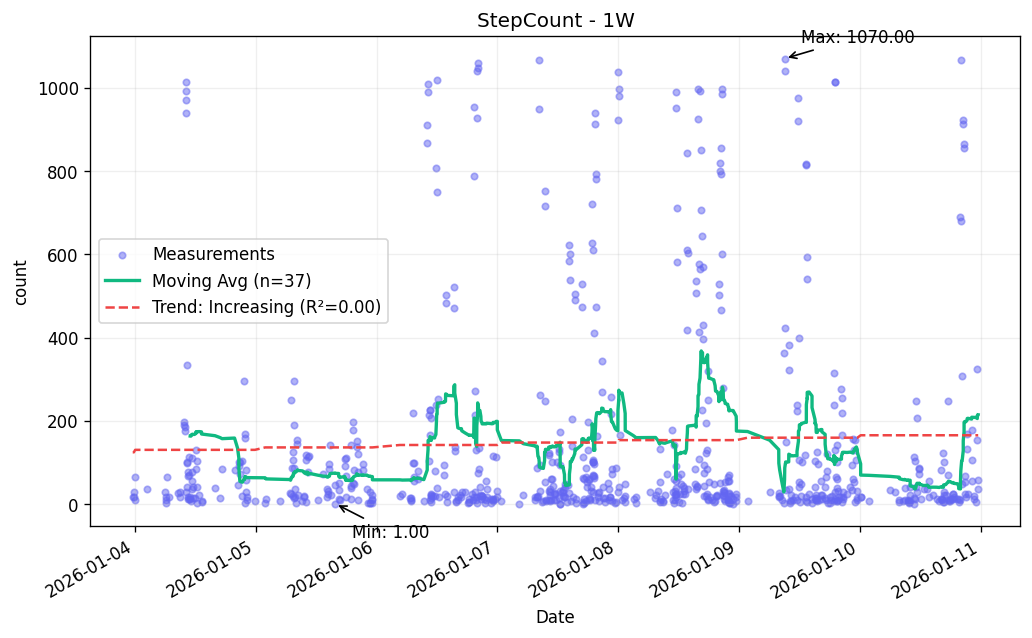
\includegraphics[width=0.95\textwidth]{plots_medical/Activity_and_Mobility/stepcount_1W.png}
\end{figure}
\begin{figure}[H]
\centering
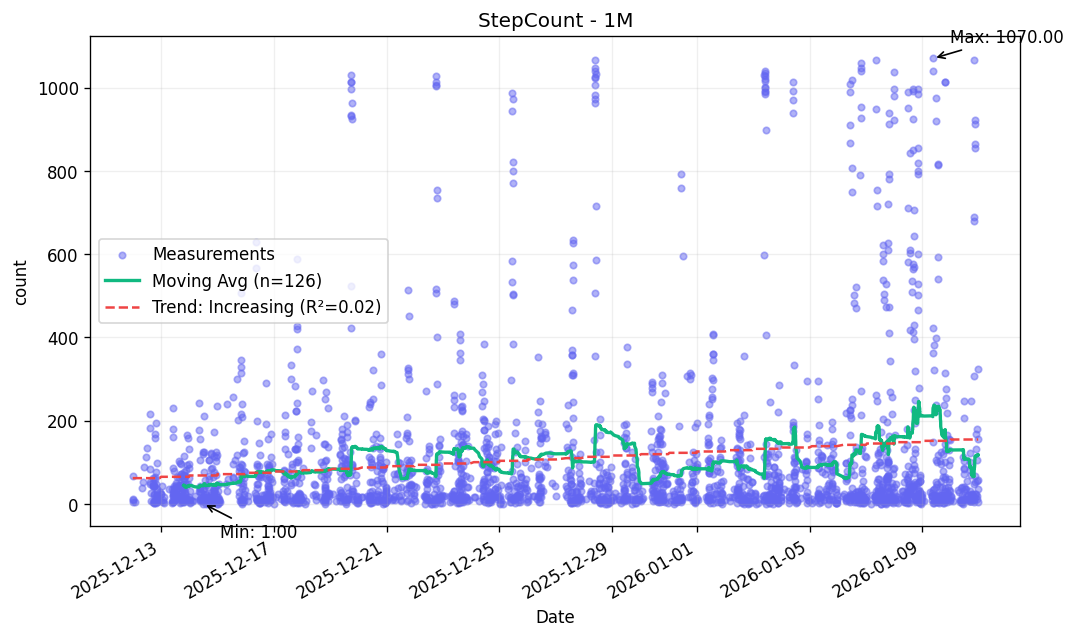
\includegraphics[width=0.95\textwidth]{plots_medical/Activity_and_Mobility/stepcount_1M.png}
\end{figure}
\begin{figure}[H]
\centering
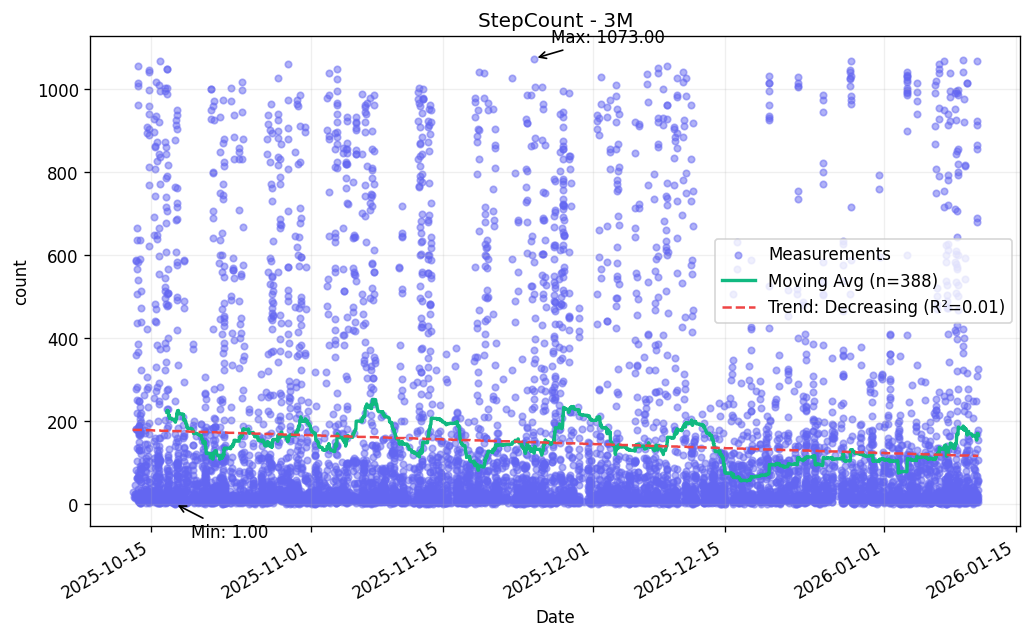
\includegraphics[width=0.95\textwidth]{plots_medical/Activity_and_Mobility/stepcount_3M.png}
\end{figure}
\begin{figure}[H]
\centering
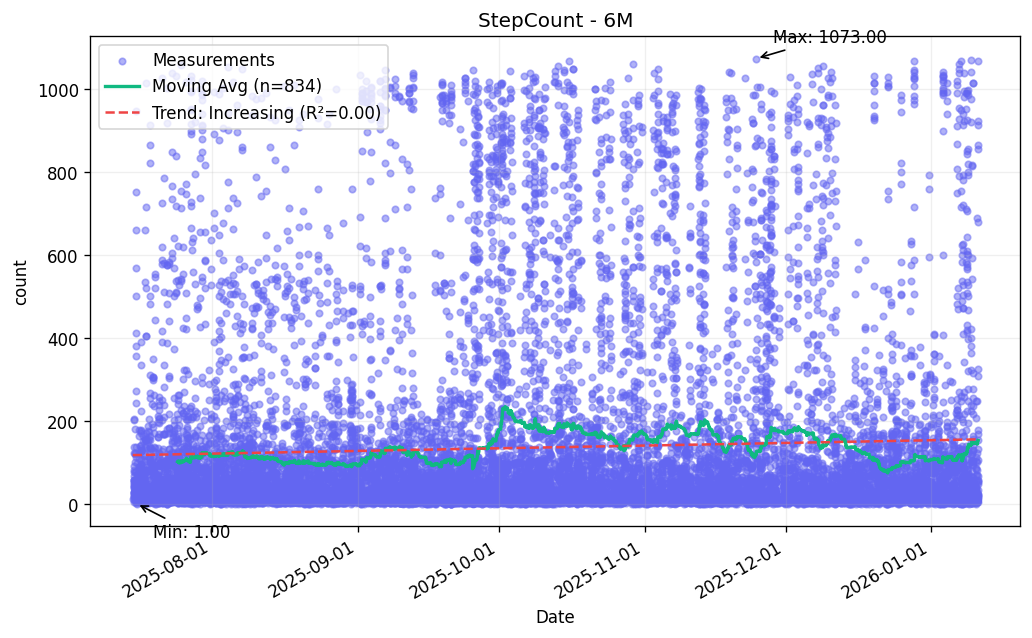
\includegraphics[width=0.95\textwidth]{plots_medical/Activity_and_Mobility/stepcount_6M.png}
\end{figure}
\begin{figure}[H]
\centering
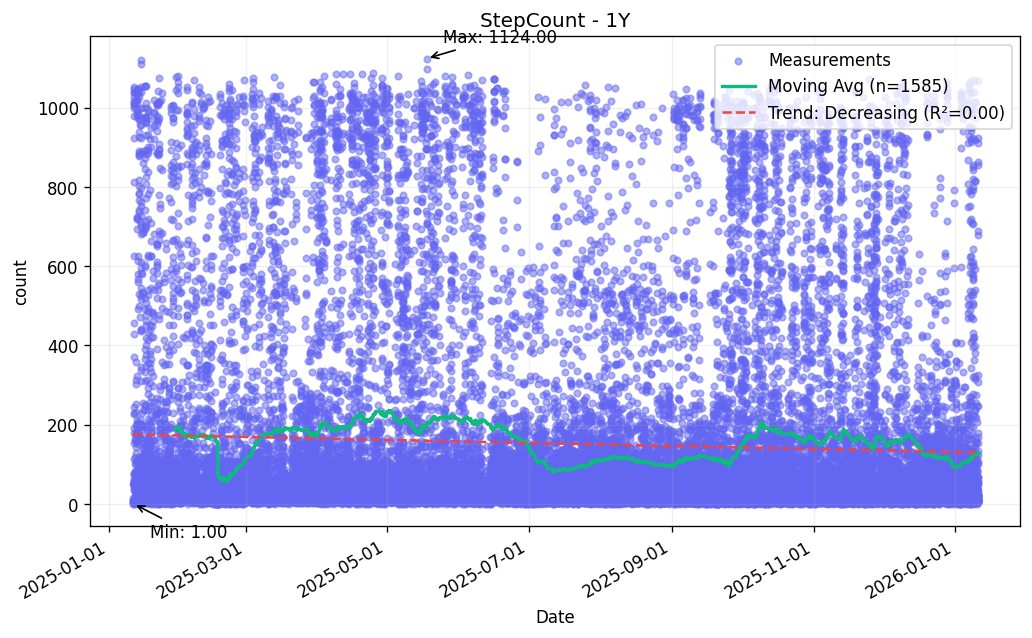
\includegraphics[width=0.95\textwidth]{plots_medical/Activity_and_Mobility/stepcount_1Y.png}
\end{figure}
\begin{figure}[H]
\centering
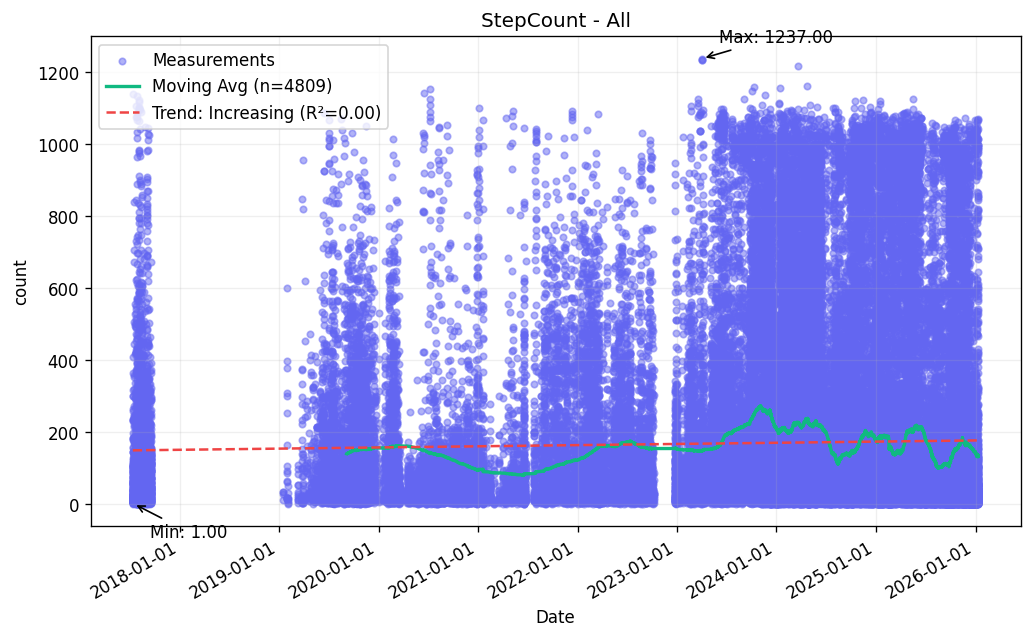
\includegraphics[width=0.95\textwidth]{plots_medical/Activity_and_Mobility/stepcount_All.png}
\end{figure}
\clearpage
\subsection{WalkingAsymmetryPercentage}
\begin{table}[H]
\centering
\resizebox{\textwidth}{!}{
\begin{tabular}{|l|c|c|c|c|c|c|}
\hline
\textbf{Window} & \textbf{Min} & \textbf{Max} & \textbf{Avg} & \textbf{Start} & \textbf{End} & \textbf{Trend Slope} \\ \hline
1W & 0.00 \% & 0.73 \% & 0.01 \% & 0.00 & 0.00 & 0.00006 \\ \hline
1M & 0.00 \% & 0.73 \% & 0.02 \% & 0.00 & 0.00 & -0.00041 \\ \hline
3M & 0.00 \% & 1.00 \% & 0.01 \% & 0.09 & 0.00 & 0.00000 \\ \hline
6M & 0.00 \% & 1.00 \% & 0.01 \% & 0.00 & 0.00 & 0.00003 \\ \hline
1Y & 0.00 \% & 1.00 \% & 0.01 \% & 0.00 & 0.00 & 0.00002 \\ \hline
All & 0.00 \% & 1.00 \% & 0.01 \% & 0.00 & 0.00 & -0.00000 \\ \hline
\end{tabular}
}
\caption{Detailed Statistics for WalkingAsymmetryPercentage}
\end{table}
\begin{figure}[H]
\centering
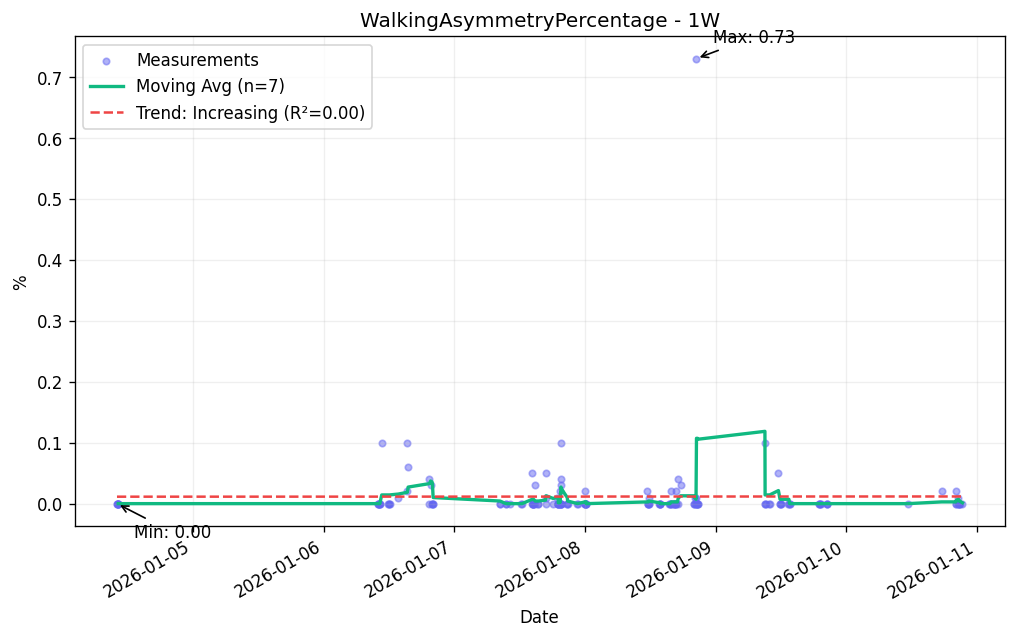
\includegraphics[width=0.95\textwidth]{plots_medical/Activity_and_Mobility/walkingasymmetrypercentage_1W.png}
\end{figure}
\begin{figure}[H]
\centering
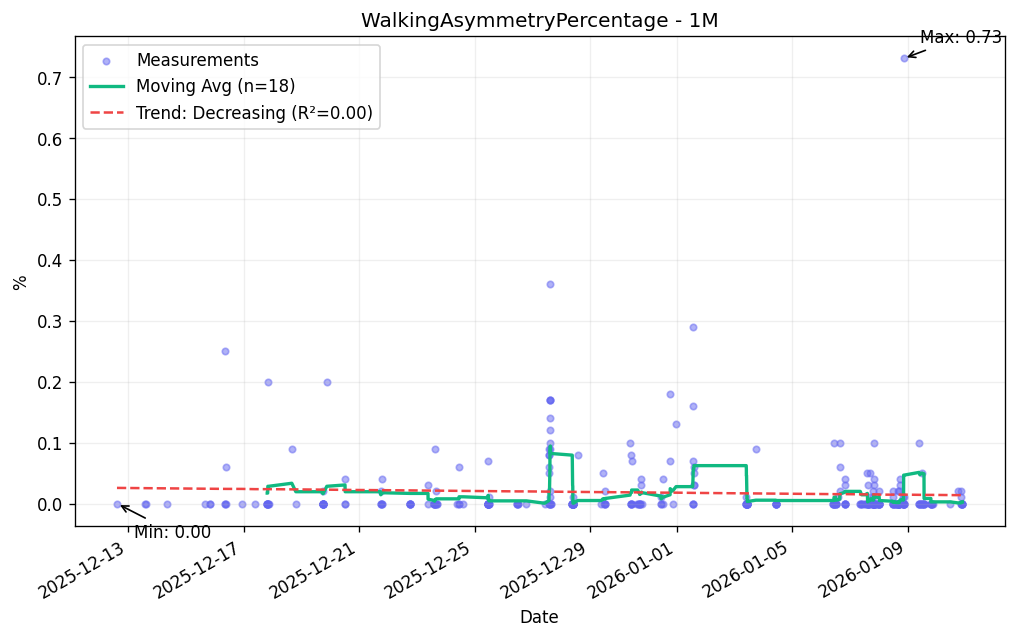
\includegraphics[width=0.95\textwidth]{plots_medical/Activity_and_Mobility/walkingasymmetrypercentage_1M.png}
\end{figure}
\begin{figure}[H]
\centering
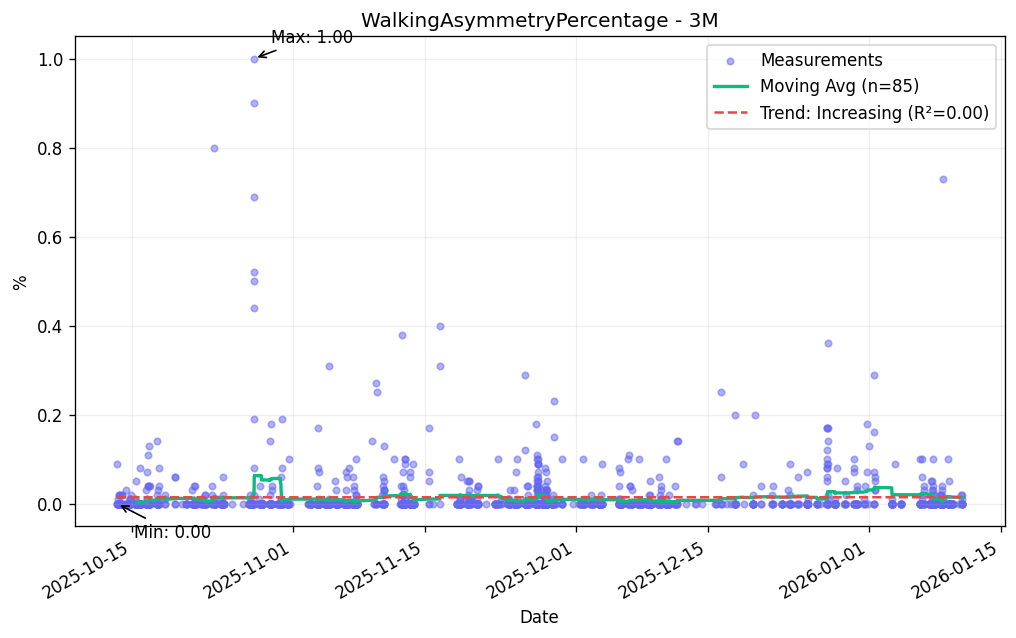
\includegraphics[width=0.95\textwidth]{plots_medical/Activity_and_Mobility/walkingasymmetrypercentage_3M.png}
\end{figure}
\begin{figure}[H]
\centering
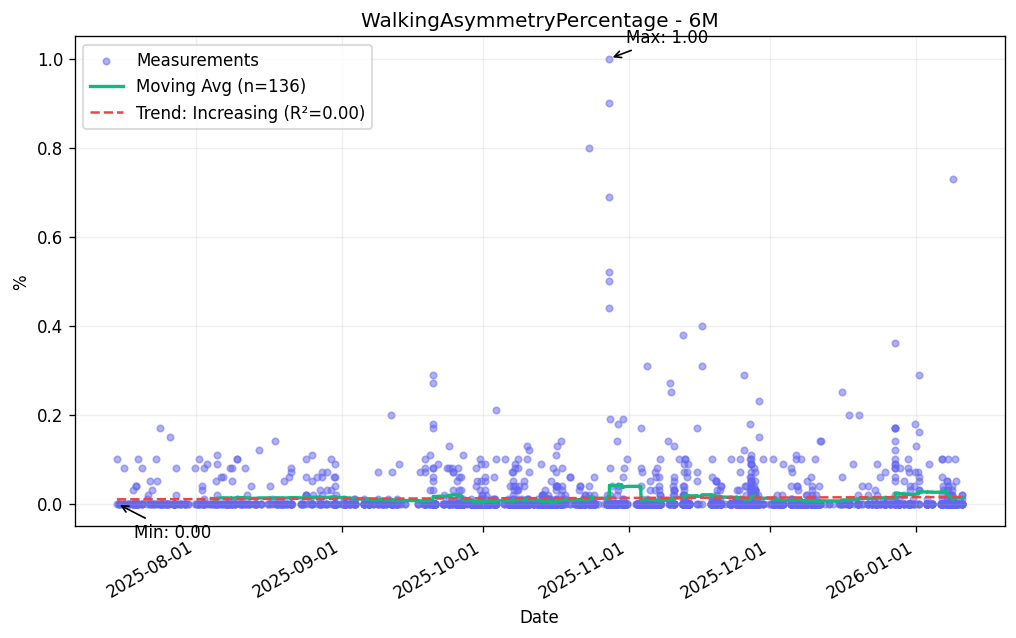
\includegraphics[width=0.95\textwidth]{plots_medical/Activity_and_Mobility/walkingasymmetrypercentage_6M.png}
\end{figure}
\begin{figure}[H]
\centering
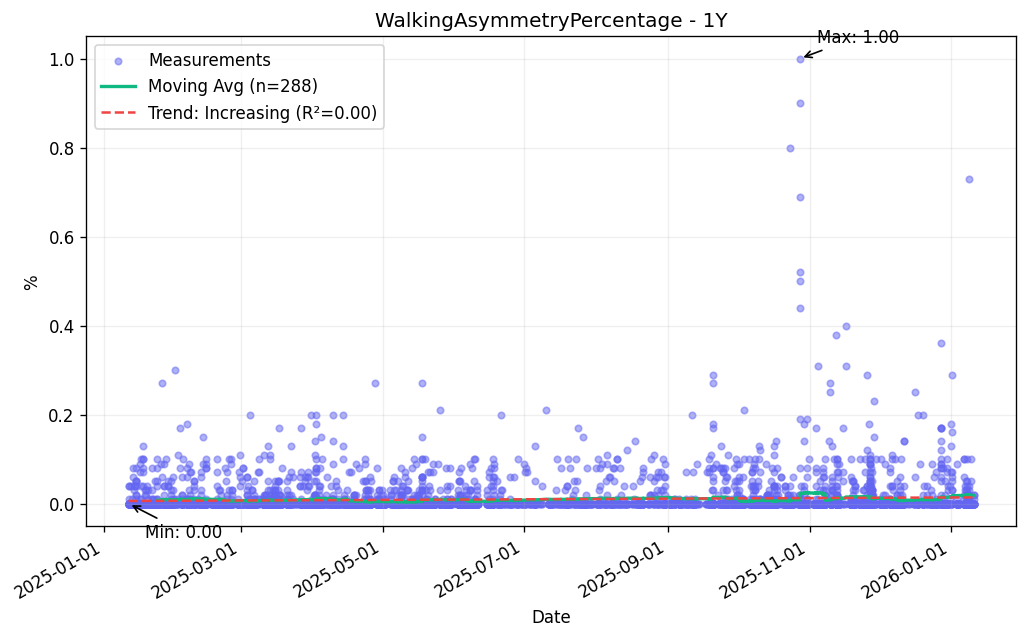
\includegraphics[width=0.95\textwidth]{plots_medical/Activity_and_Mobility/walkingasymmetrypercentage_1Y.png}
\end{figure}
\begin{figure}[H]
\centering
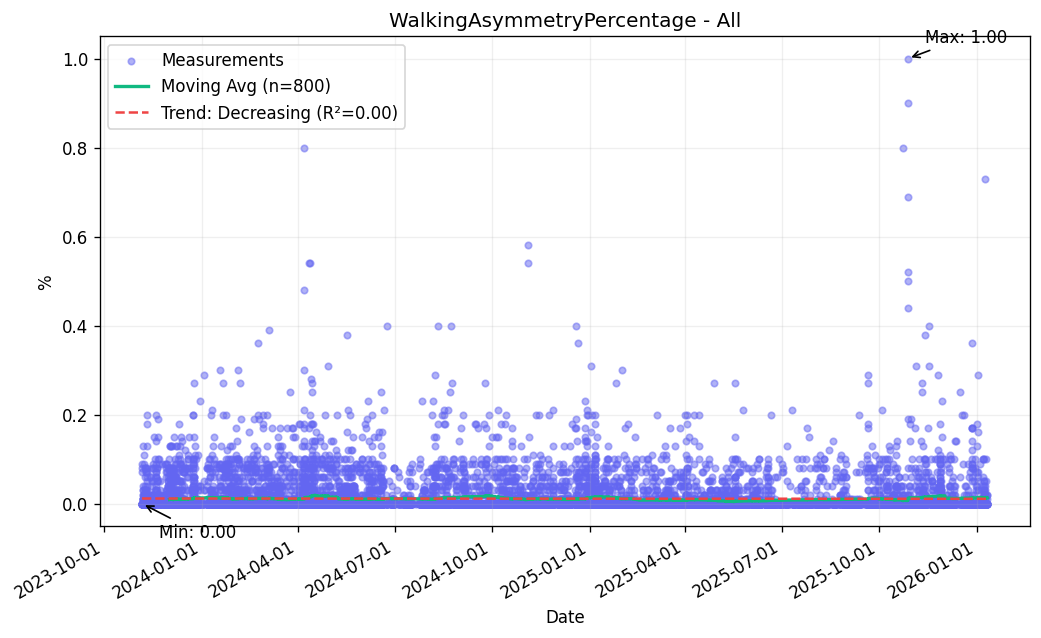
\includegraphics[width=0.95\textwidth]{plots_medical/Activity_and_Mobility/walkingasymmetrypercentage_All.png}
\end{figure}
\clearpage
\subsection{WalkingDoubleSupportPercentage}
\begin{table}[H]
\centering
\resizebox{\textwidth}{!}{
\begin{tabular}{|l|c|c|c|c|c|c|}
\hline
\textbf{Window} & \textbf{Min} & \textbf{Max} & \textbf{Avg} & \textbf{Start} & \textbf{End} & \textbf{Trend Slope} \\ \hline
1W & 0.24 \% & 0.34 \% & 0.29 \% & 0.31 & 0.29 & -0.00215 \\ \hline
1M & 0.24 \% & 0.34 \% & 0.30 \% & 0.30 & 0.29 & -0.00056 \\ \hline
3M & 0.23 \% & 0.35 \% & 0.30 \% & 0.29 & 0.29 & 0.00005 \\ \hline
6M & 0.23 \% & 0.35 \% & 0.30 \% & 0.30 & 0.29 & -0.00003 \\ \hline
1Y & 0.23 \% & 0.36 \% & 0.30 \% & 0.34 & 0.29 & -0.00001 \\ \hline
All & 0.22 \% & 0.36 \% & 0.30 \% & 0.31 & 0.29 & 0.00001 \\ \hline
\end{tabular}
}
\caption{Detailed Statistics for WalkingDoubleSupportPercentage}
\end{table}
\begin{figure}[H]
\centering
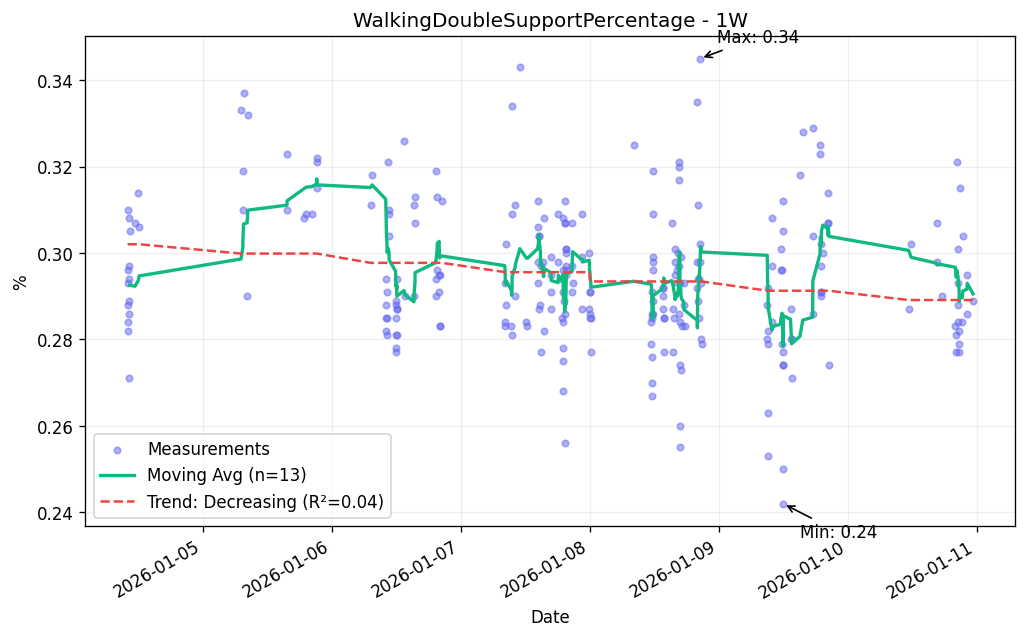
\includegraphics[width=0.95\textwidth]{plots_medical/Activity_and_Mobility/walkingdoublesupportpercentage_1W.png}
\end{figure}
\begin{figure}[H]
\centering
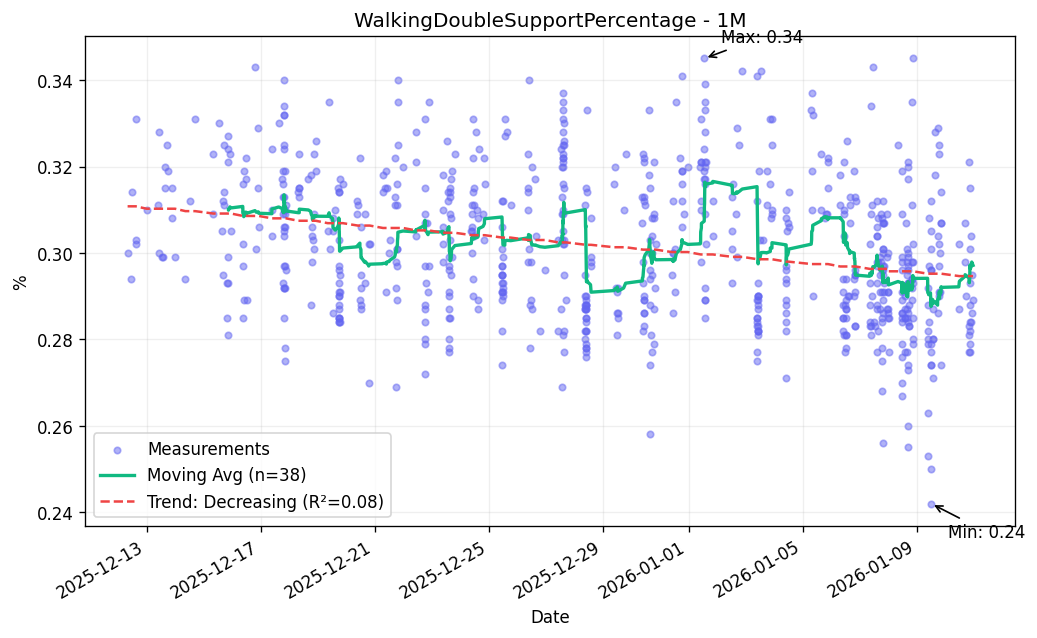
\includegraphics[width=0.95\textwidth]{plots_medical/Activity_and_Mobility/walkingdoublesupportpercentage_1M.png}
\end{figure}
\begin{figure}[H]
\centering
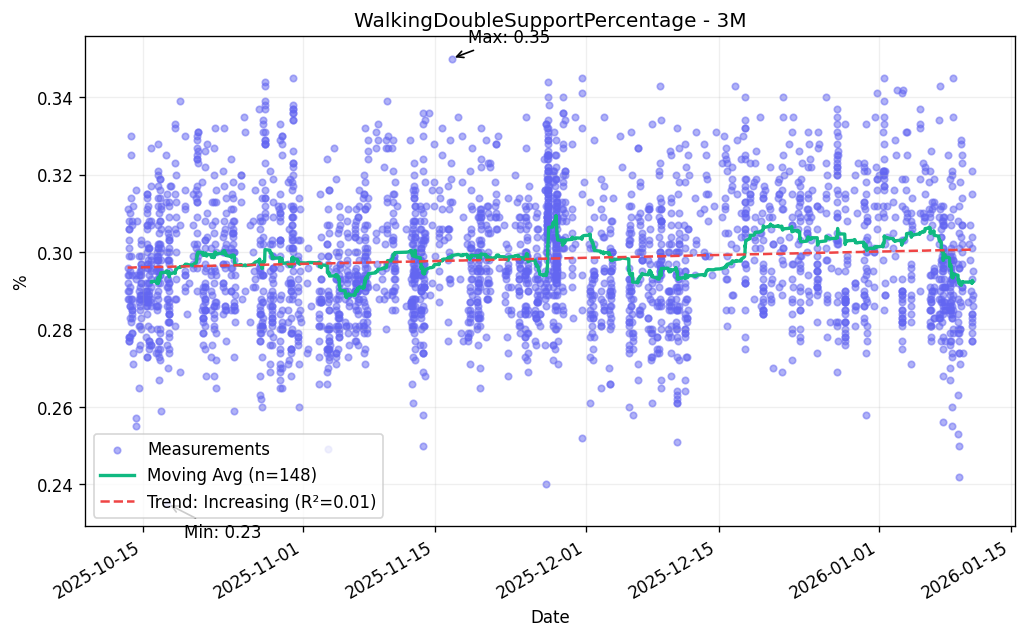
\includegraphics[width=0.95\textwidth]{plots_medical/Activity_and_Mobility/walkingdoublesupportpercentage_3M.png}
\end{figure}
\begin{figure}[H]
\centering
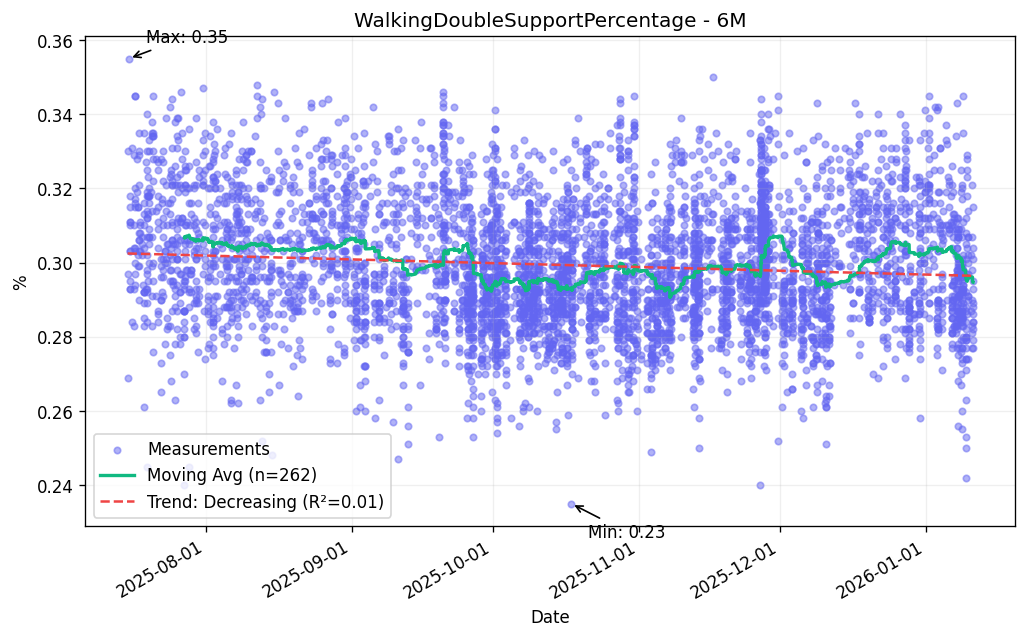
\includegraphics[width=0.95\textwidth]{plots_medical/Activity_and_Mobility/walkingdoublesupportpercentage_6M.png}
\end{figure}
\begin{figure}[H]
\centering
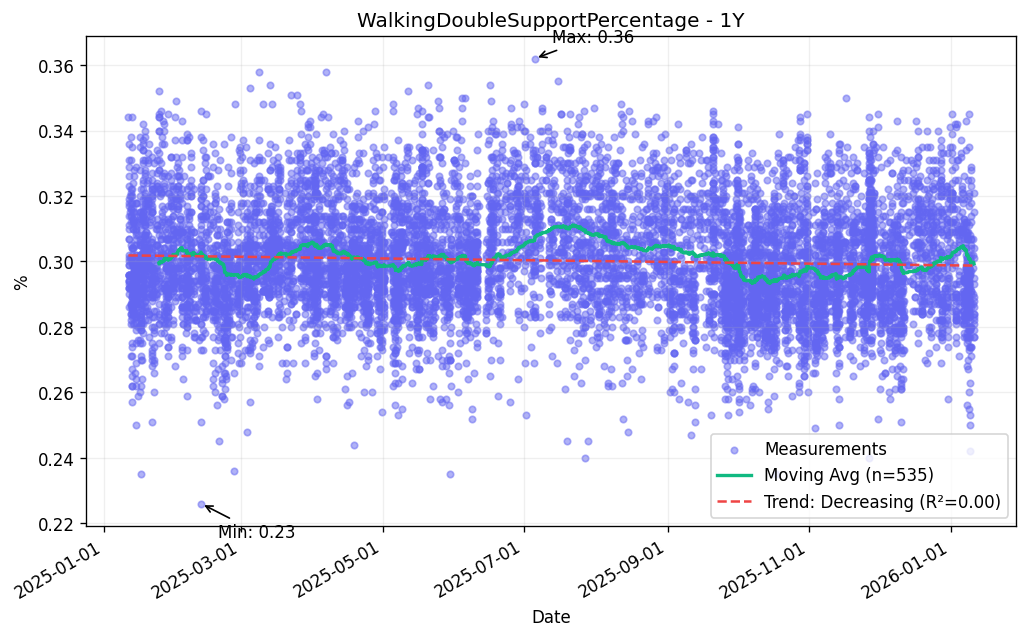
\includegraphics[width=0.95\textwidth]{plots_medical/Activity_and_Mobility/walkingdoublesupportpercentage_1Y.png}
\end{figure}
\begin{figure}[H]
\centering
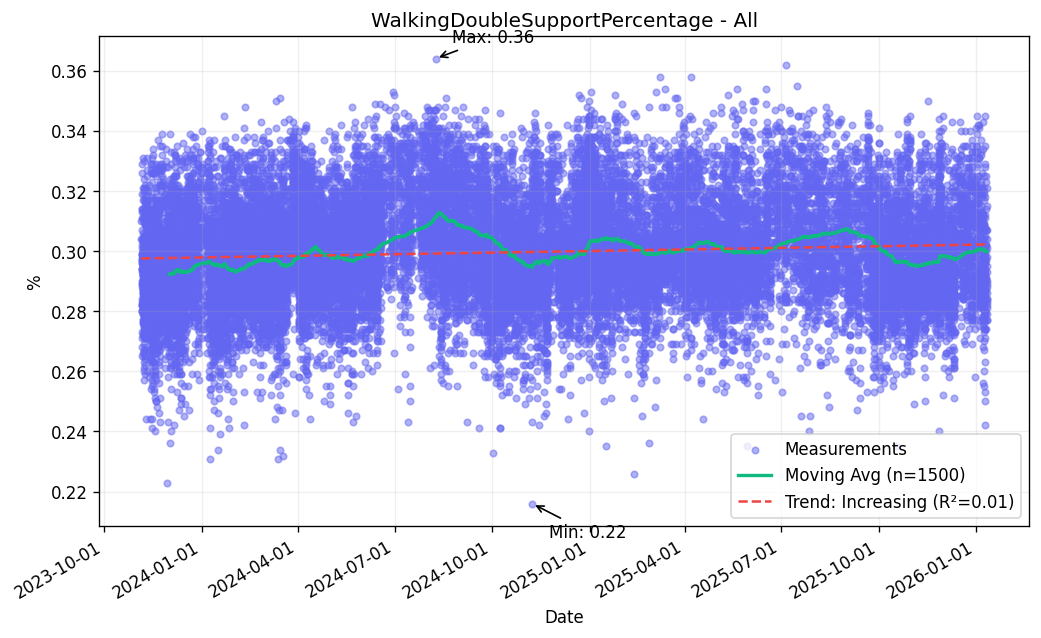
\includegraphics[width=0.95\textwidth]{plots_medical/Activity_and_Mobility/walkingdoublesupportpercentage_All.png}
\end{figure}
\clearpage
\subsection{WalkingSpeed}
\begin{table}[H]
\centering
\resizebox{\textwidth}{!}{
\begin{tabular}{|l|c|c|c|c|c|c|}
\hline
\textbf{Window} & \textbf{Min} & \textbf{Max} & \textbf{Avg} & \textbf{Start} & \textbf{End} & \textbf{Trend Slope} \\ \hline
1W & 1.39 mi/hr & 4.23 mi/hr & 2.87 mi/hr & 2.46 & 3.00 & 0.05449 \\ \hline
1M & 1.16 mi/hr & 4.23 mi/hr & 2.61 mi/hr & 2.66 & 3.00 & 0.02278 \\ \hline
3M & 0.94 mi/hr & 4.34 mi/hr & 2.69 mi/hr & 2.93 & 3.00 & -0.00088 \\ \hline
6M & 0.94 mi/hr & 4.45 mi/hr & 2.69 mi/hr & 2.95 & 3.00 & 0.00039 \\ \hline
1Y & 0.94 mi/hr & 4.61 mi/hr & 2.75 mi/hr & 1.72 & 3.00 & -0.00045 \\ \hline
All & 0.92 mi/hr & 4.68 mi/hr & 2.67 mi/hr & 2.08 & 3.00 & 0.00013 \\ \hline
\end{tabular}
}
\caption{Detailed Statistics for WalkingSpeed}
\end{table}
\begin{figure}[H]
\centering
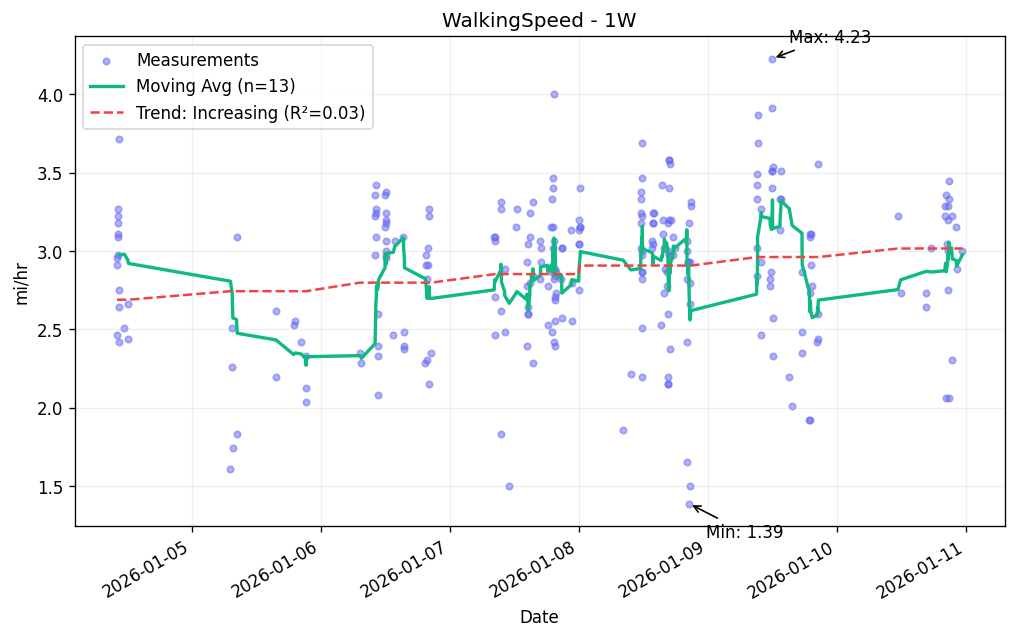
\includegraphics[width=0.95\textwidth]{plots_medical/Activity_and_Mobility/walkingspeed_1W.png}
\end{figure}
\begin{figure}[H]
\centering
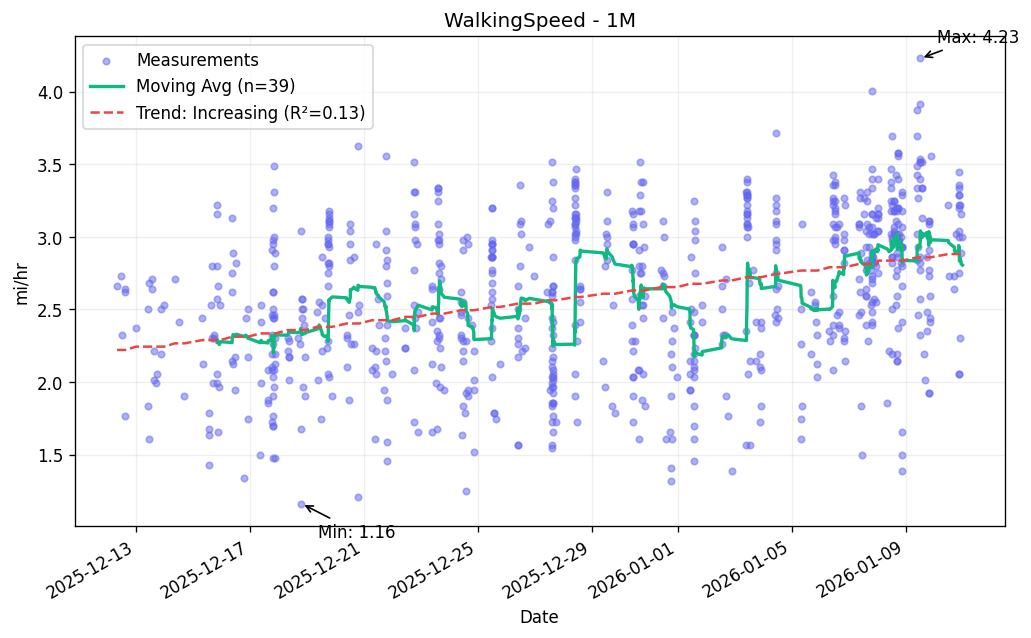
\includegraphics[width=0.95\textwidth]{plots_medical/Activity_and_Mobility/walkingspeed_1M.png}
\end{figure}
\begin{figure}[H]
\centering
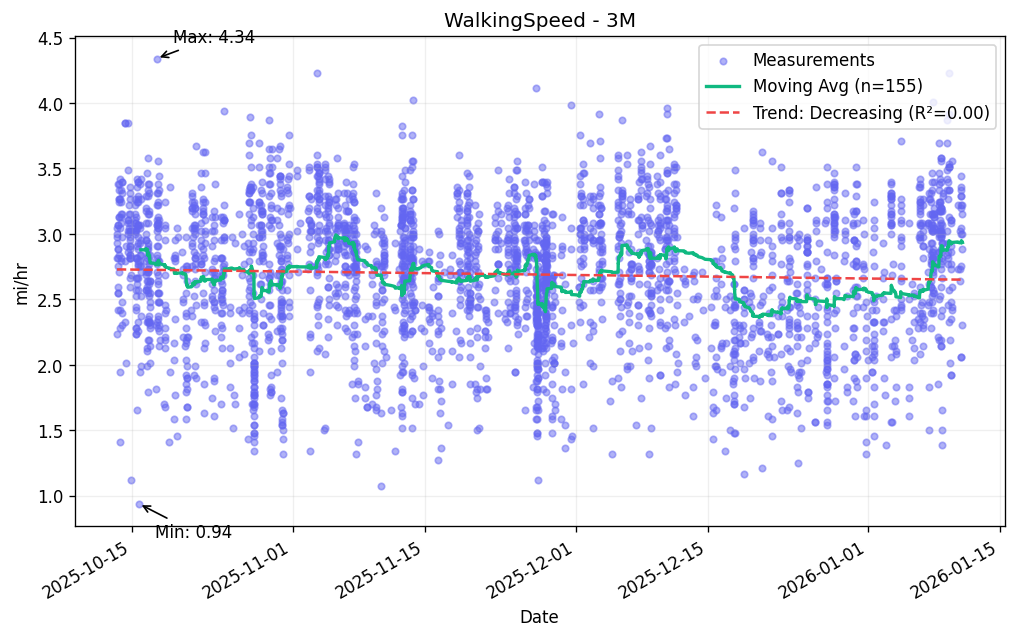
\includegraphics[width=0.95\textwidth]{plots_medical/Activity_and_Mobility/walkingspeed_3M.png}
\end{figure}
\begin{figure}[H]
\centering
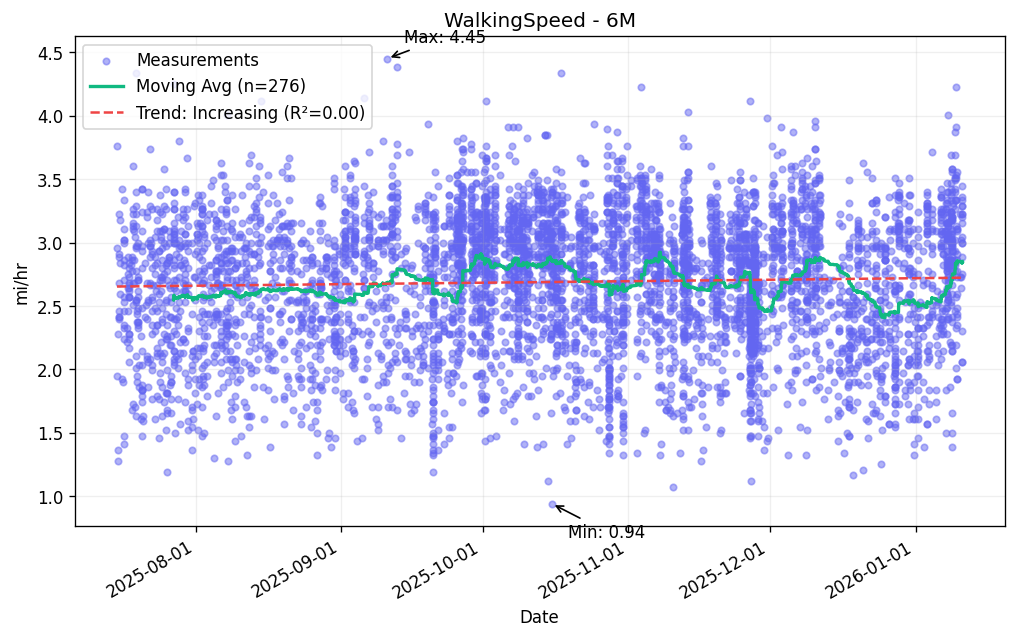
\includegraphics[width=0.95\textwidth]{plots_medical/Activity_and_Mobility/walkingspeed_6M.png}
\end{figure}
\begin{figure}[H]
\centering
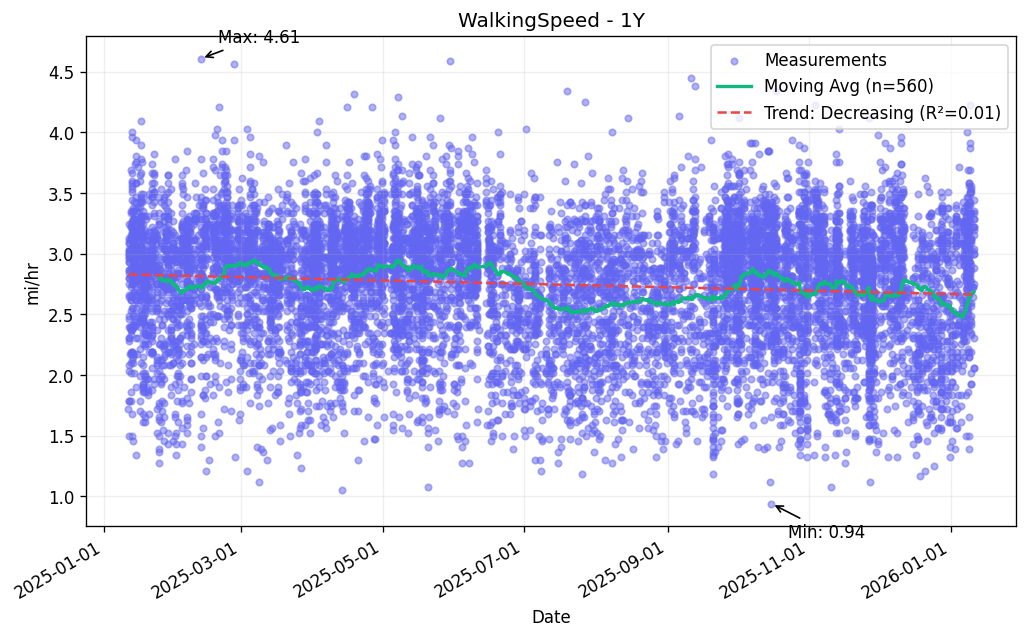
\includegraphics[width=0.95\textwidth]{plots_medical/Activity_and_Mobility/walkingspeed_1Y.png}
\end{figure}
\begin{figure}[H]
\centering
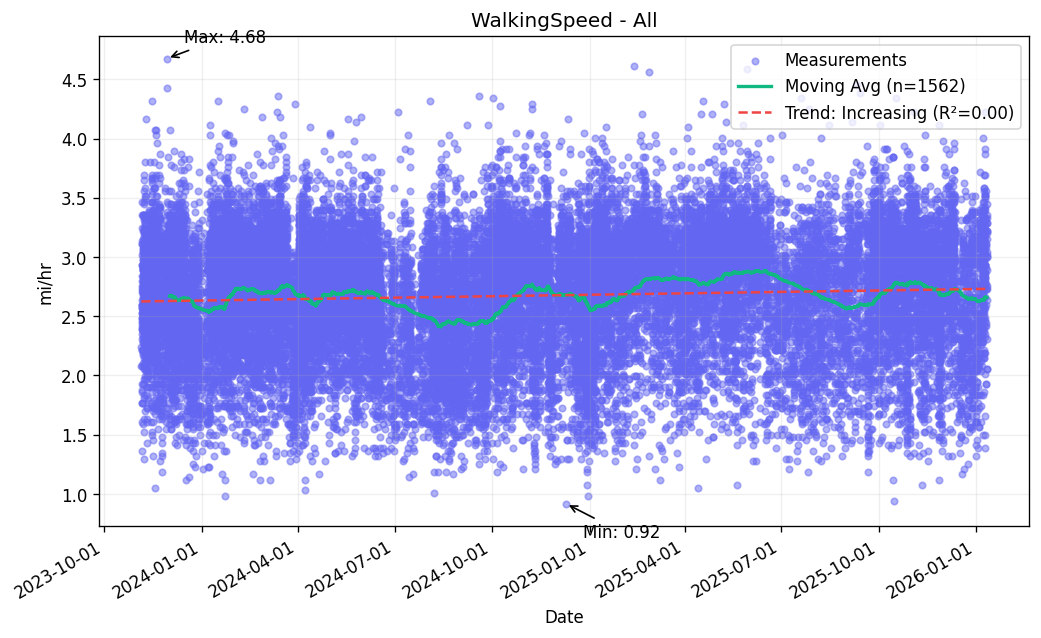
\includegraphics[width=0.95\textwidth]{plots_medical/Activity_and_Mobility/walkingspeed_All.png}
\end{figure}
\clearpage
\subsection{WalkingStepLength}
\begin{table}[H]
\centering
\resizebox{\textwidth}{!}{
\begin{tabular}{|l|c|c|c|c|c|c|}
\hline
\textbf{Window} & \textbf{Min} & \textbf{Max} & \textbf{Avg} & \textbf{Start} & \textbf{End} & \textbf{Trend Slope} \\ \hline
1W & 17.72 in & 40.94 in & 29.14 in & 26.38 & 30.32 & 0.37842 \\ \hline
1M & 14.96 in & 40.94 in & 27.01 in & 27.17 & 30.32 & 0.17736 \\ \hline
3M & 13.78 in & 44.09 in & 27.84 in & 29.53 & 30.32 & -0.01049 \\ \hline
6M & 12.99 in & 44.88 in & 27.92 in & 29.92 & 30.32 & 0.00073 \\ \hline
1Y & 12.99 in & 45.28 in & 28.19 in & 18.11 & 30.32 & -0.00211 \\ \hline
All & 9.06 in & 53.15 in & 27.42 in & 23.23 & 30.32 & 0.00193 \\ \hline
\end{tabular}
}
\caption{Detailed Statistics for WalkingStepLength}
\end{table}
\begin{figure}[H]
\centering
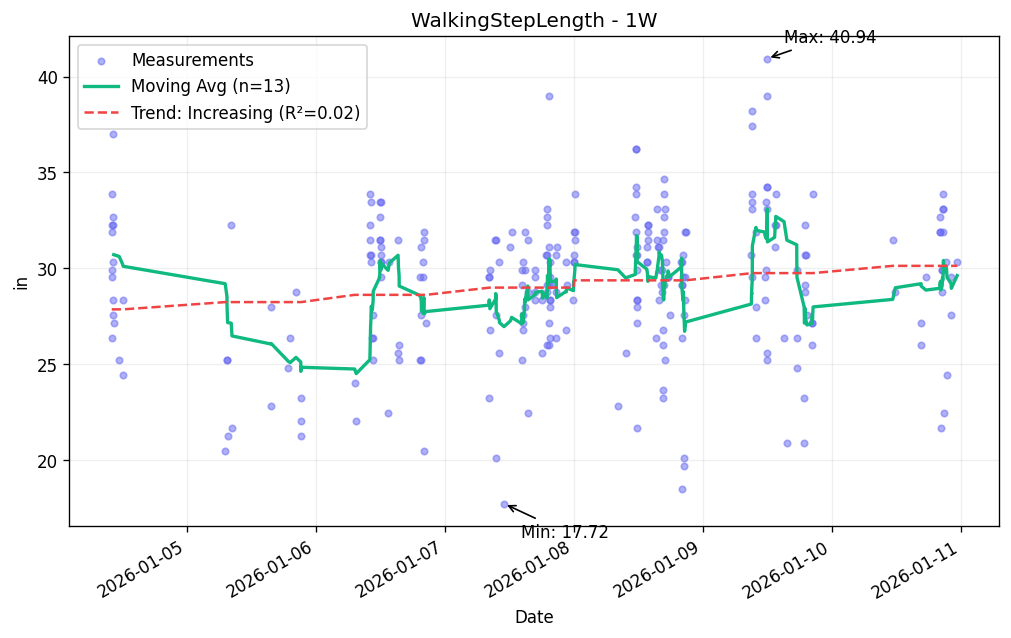
\includegraphics[width=0.95\textwidth]{plots_medical/Activity_and_Mobility/walkingsteplength_1W.png}
\end{figure}
\begin{figure}[H]
\centering
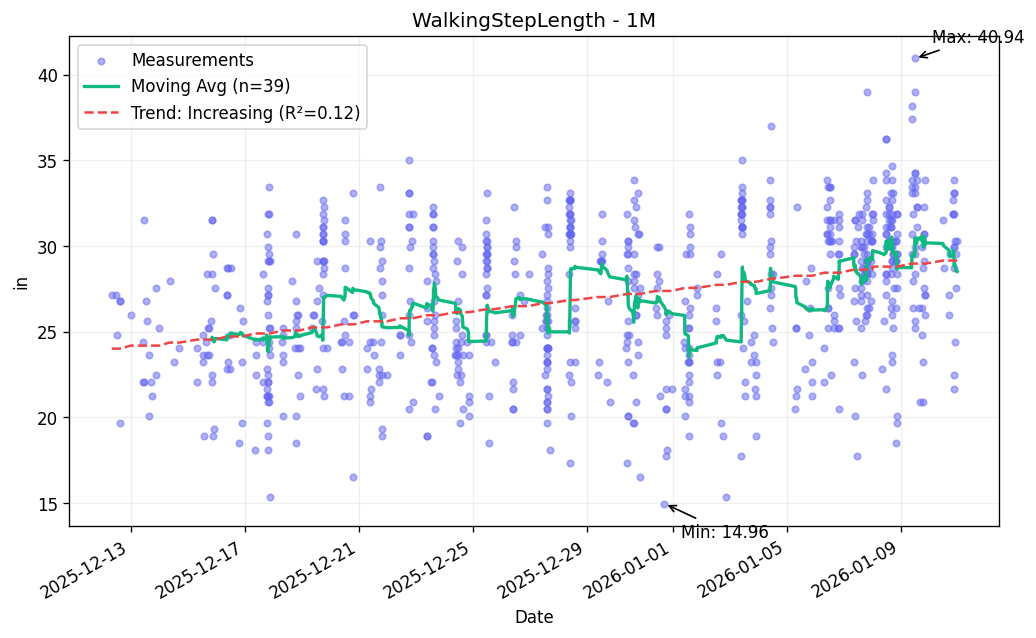
\includegraphics[width=0.95\textwidth]{plots_medical/Activity_and_Mobility/walkingsteplength_1M.png}
\end{figure}
\begin{figure}[H]
\centering
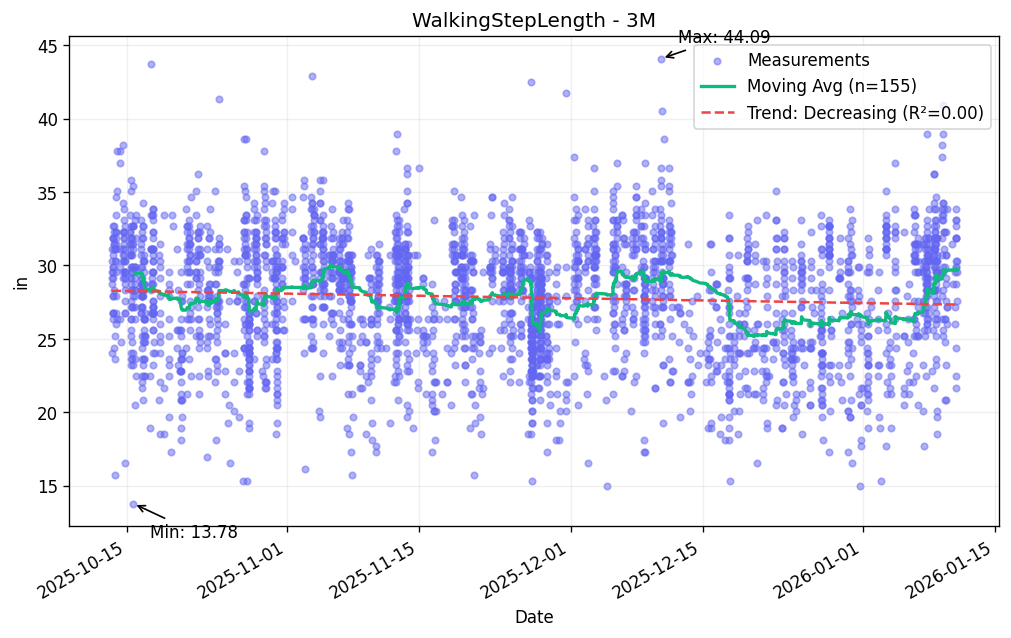
\includegraphics[width=0.95\textwidth]{plots_medical/Activity_and_Mobility/walkingsteplength_3M.png}
\end{figure}
\begin{figure}[H]
\centering
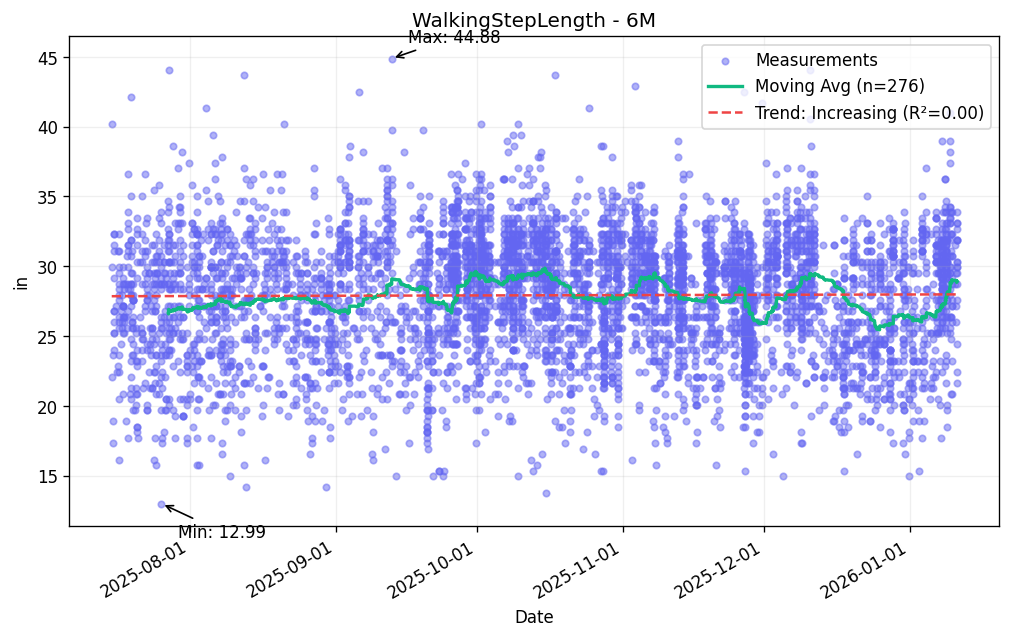
\includegraphics[width=0.95\textwidth]{plots_medical/Activity_and_Mobility/walkingsteplength_6M.png}
\end{figure}
\begin{figure}[H]
\centering
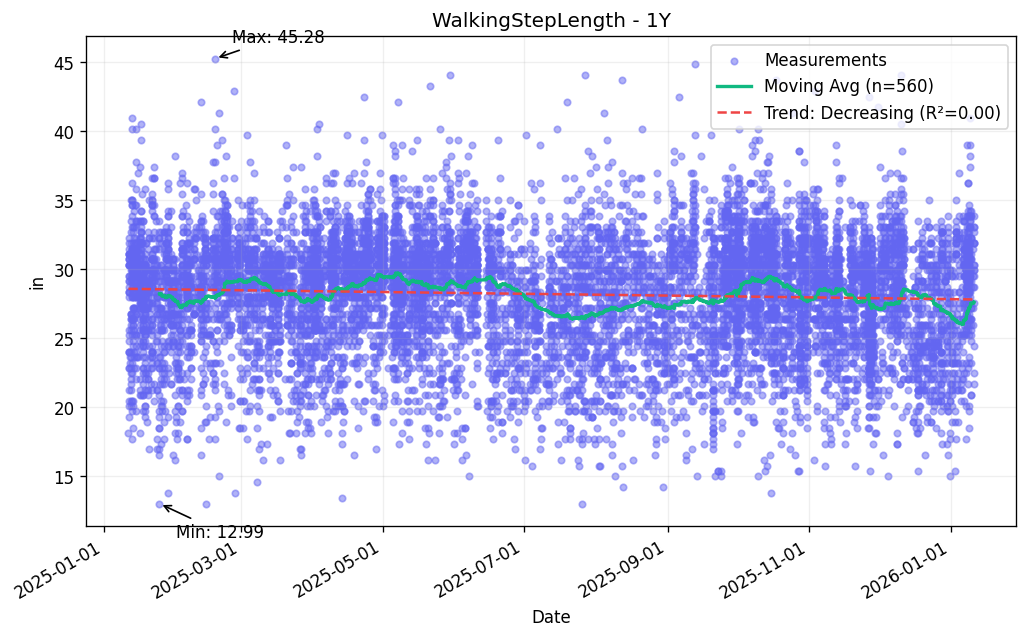
\includegraphics[width=0.95\textwidth]{plots_medical/Activity_and_Mobility/walkingsteplength_1Y.png}
\end{figure}
\begin{figure}[H]
\centering
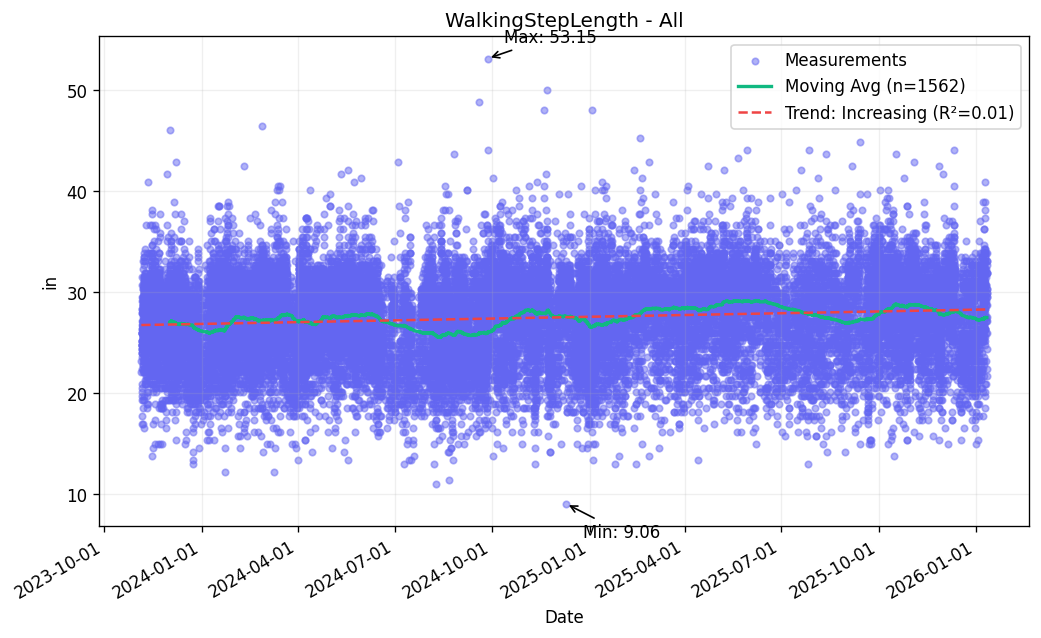
\includegraphics[width=0.95\textwidth]{plots_medical/Activity_and_Mobility/walkingsteplength_All.png}
\end{figure}
\clearpage
\section{Nutrition}
\subsection{DietaryCarbohydrates}
\begin{table}[H]
\centering
\resizebox{\textwidth}{!}{
\begin{tabular}{|l|c|c|c|c|c|c|}
\hline
\textbf{Window} & \textbf{Min} & \textbf{Max} & \textbf{Avg} & \textbf{Start} & \textbf{End} & \textbf{Trend Slope} \\ \hline
1W & 0.00 g & 108.00 g & 35.62 g & 108.00 & 2.00 & -6.88289 \\ \hline
1M & 0.00 g & 108.00 g & 35.62 g & 108.00 & 2.00 & -6.88289 \\ \hline
3M & 0.00 g & 108.00 g & 36.18 g & 57.00 & 2.00 & -0.18844 \\ \hline
6M & 0.00 g & 210.00 g & 45.69 g & 27.00 & 2.00 & -0.01960 \\ \hline
1Y & 0.00 g & 210.00 g & 38.19 g & 55.25 & 2.00 & 0.06834 \\ \hline
All & 0.00 g & 252.63 g & 37.37 g & 33.18 & 2.00 & 0.02095 \\ \hline
\end{tabular}
}
\caption{Detailed Statistics for DietaryCarbohydrates}
\end{table}
\begin{figure}[H]
\centering
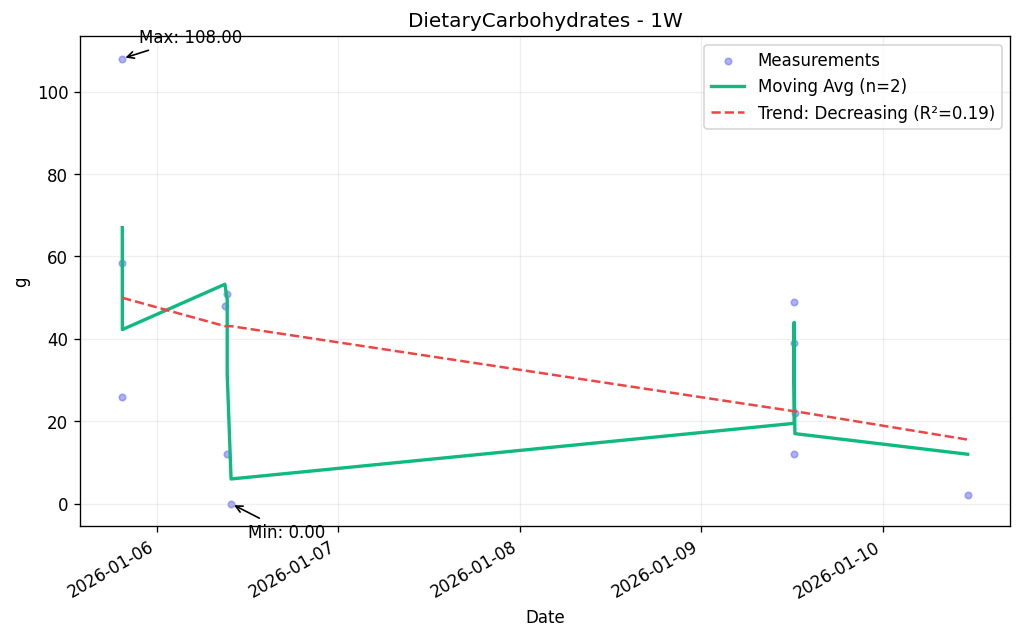
\includegraphics[width=0.95\textwidth]{plots_medical/Nutrition/dietarycarbohydrates_1W.png}
\end{figure}
\begin{figure}[H]
\centering
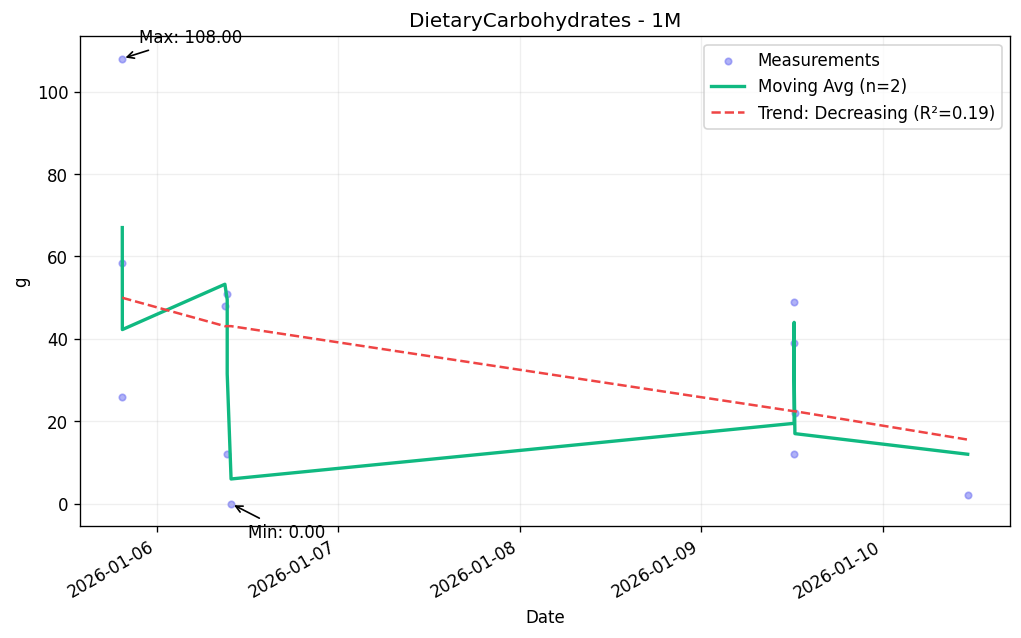
\includegraphics[width=0.95\textwidth]{plots_medical/Nutrition/dietarycarbohydrates_1M.png}
\end{figure}
\begin{figure}[H]
\centering
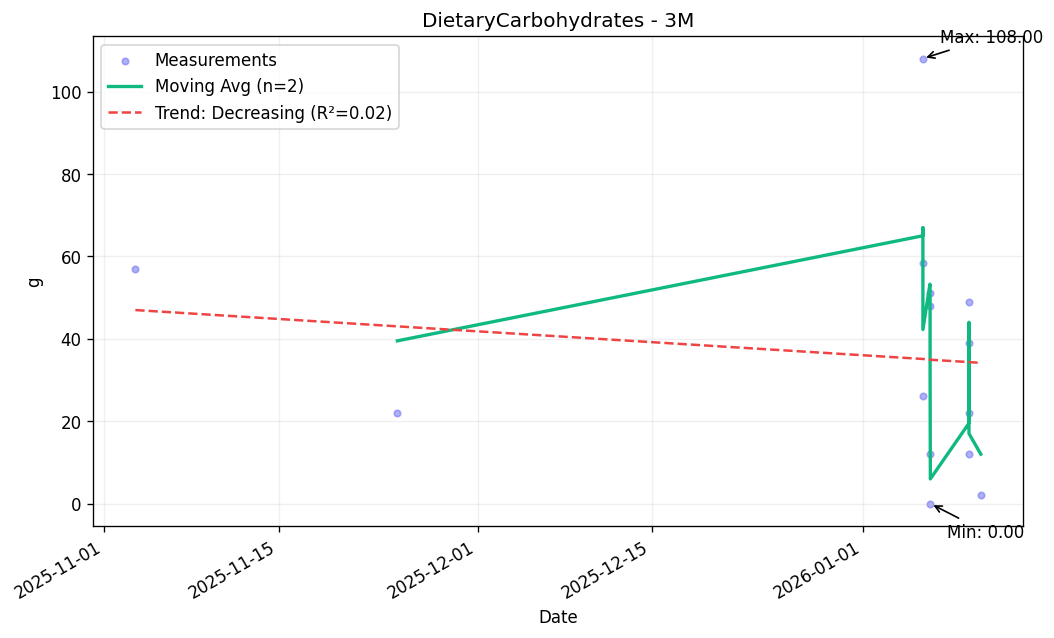
\includegraphics[width=0.95\textwidth]{plots_medical/Nutrition/dietarycarbohydrates_3M.png}
\end{figure}
\begin{figure}[H]
\centering
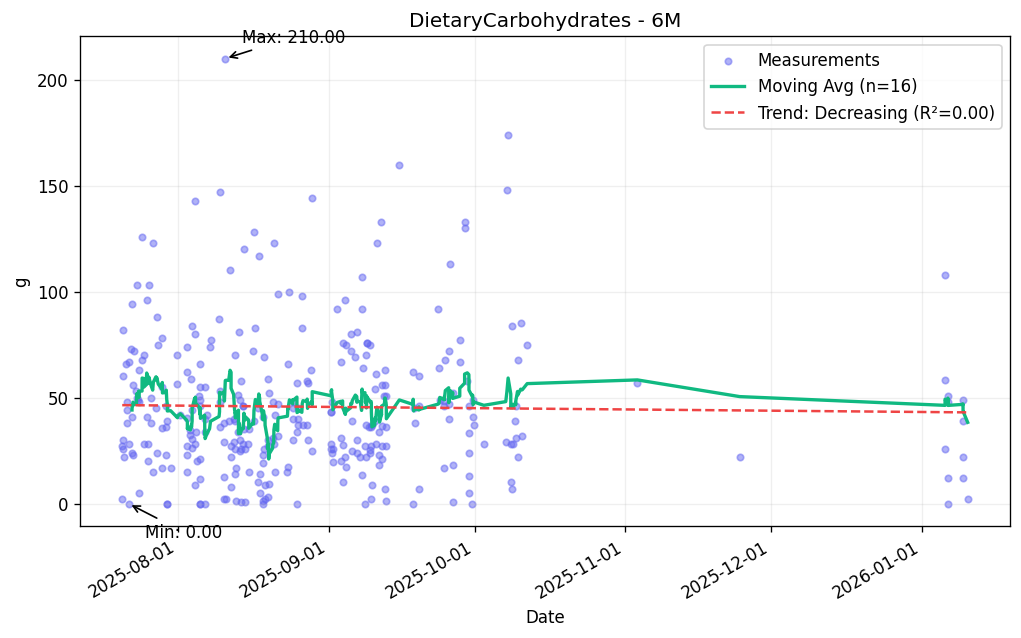
\includegraphics[width=0.95\textwidth]{plots_medical/Nutrition/dietarycarbohydrates_6M.png}
\end{figure}
\begin{figure}[H]
\centering
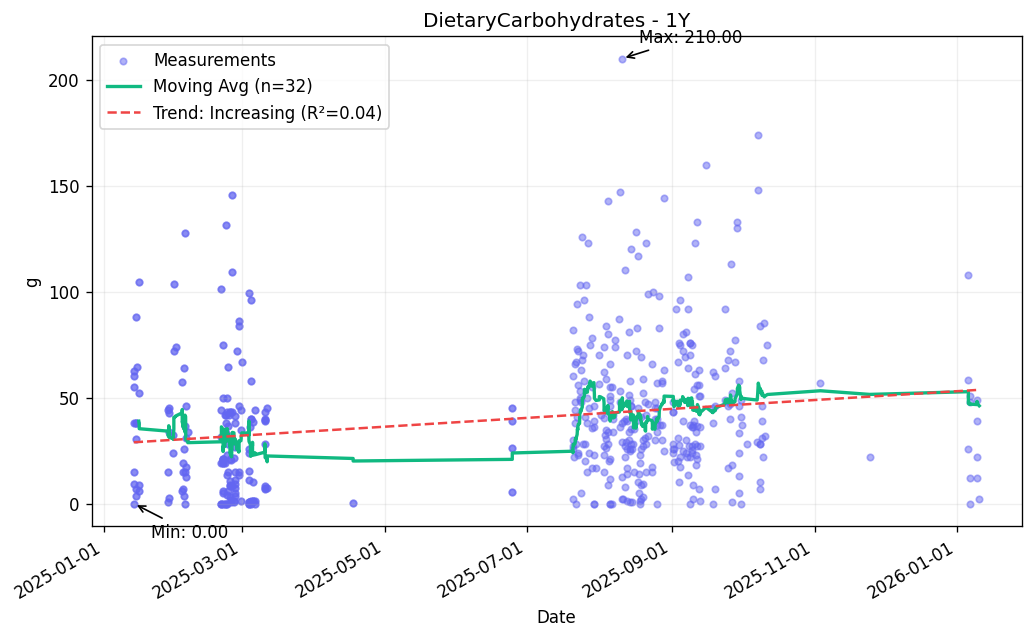
\includegraphics[width=0.95\textwidth]{plots_medical/Nutrition/dietarycarbohydrates_1Y.png}
\end{figure}
\begin{figure}[H]
\centering
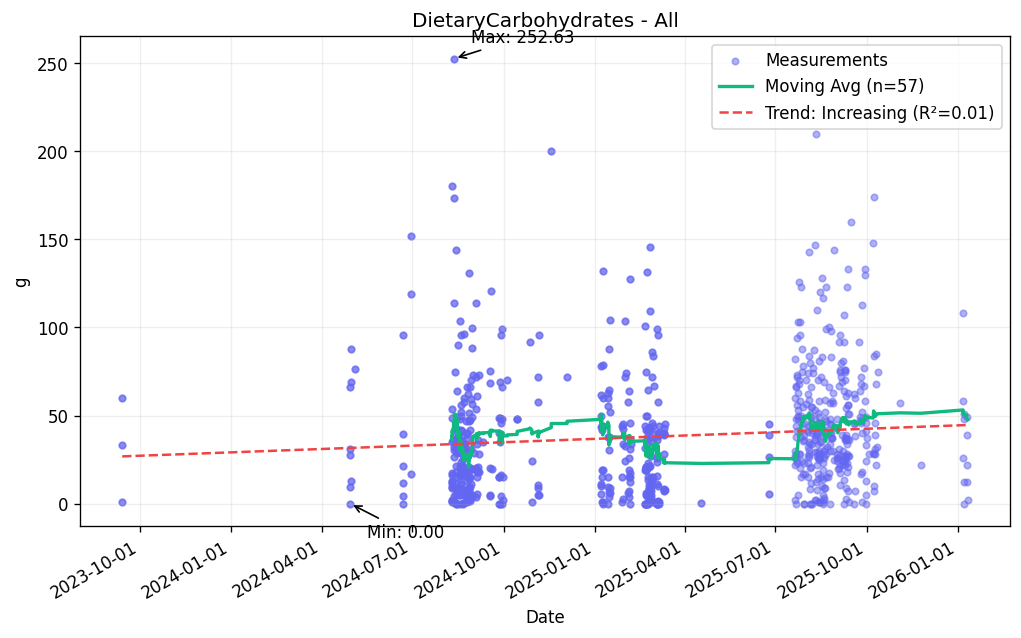
\includegraphics[width=0.95\textwidth]{plots_medical/Nutrition/dietarycarbohydrates_All.png}
\end{figure}
\clearpage
\subsection{DietaryEnergyConsumed}
\begin{table}[H]
\centering
\resizebox{\textwidth}{!}{
\begin{tabular}{|l|c|c|c|c|c|c|}
\hline
\textbf{Window} & \textbf{Min} & \textbf{Max} & \textbf{Avg} & \textbf{Start} & \textbf{End} & \textbf{Trend Slope} \\ \hline
1W & 130.00 Cal & 920.00 Cal & 316.38 Cal & 920.00 & 260.00 & -32.36762 \\ \hline
1M & 130.00 Cal & 920.00 Cal & 316.38 Cal & 920.00 & 260.00 & -32.36762 \\ \hline
3M & 130.00 Cal & 920.00 Cal & 311.18 Cal & 310.00 & 260.00 & 0.26994 \\ \hline
6M & 0.00 Cal & 1420.00 Cal & 352.55 Cal & 105.00 & 260.00 & 0.14780 \\ \hline
1Y & 0.00 Cal & 1420.00 Cal & 311.69 Cal & 403.00 & 260.00 & 0.39122 \\ \hline
All & 0.00 Cal & 2273.68 Cal & 291.51 Cal & 166.60 & 260.00 & 0.22769 \\ \hline
\end{tabular}
}
\caption{Detailed Statistics for DietaryEnergyConsumed}
\end{table}
\begin{figure}[H]
\centering
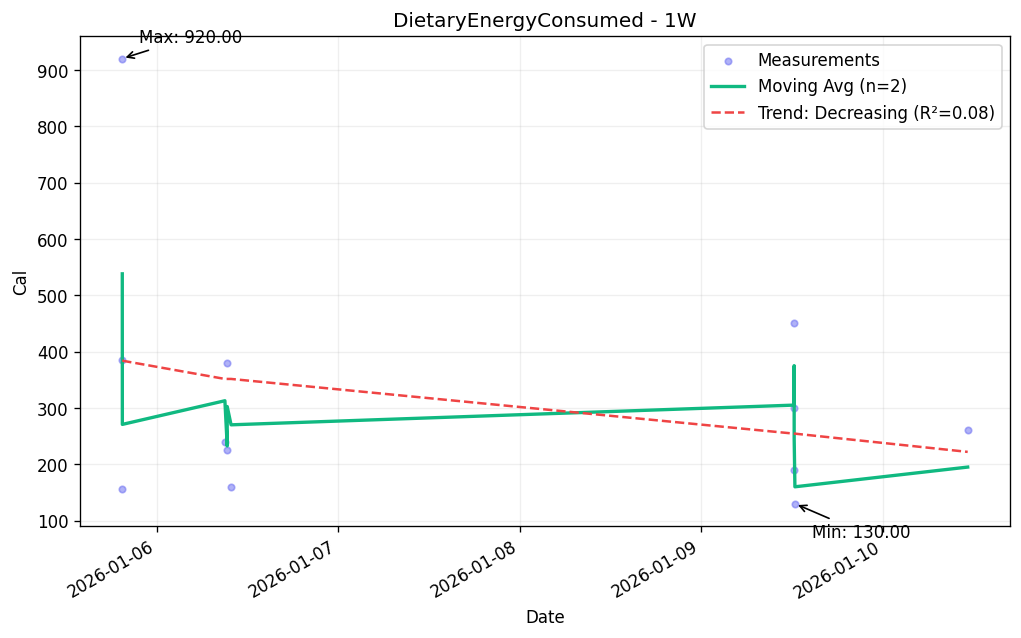
\includegraphics[width=0.95\textwidth]{plots_medical/Nutrition/dietaryenergyconsumed_1W.png}
\end{figure}
\begin{figure}[H]
\centering
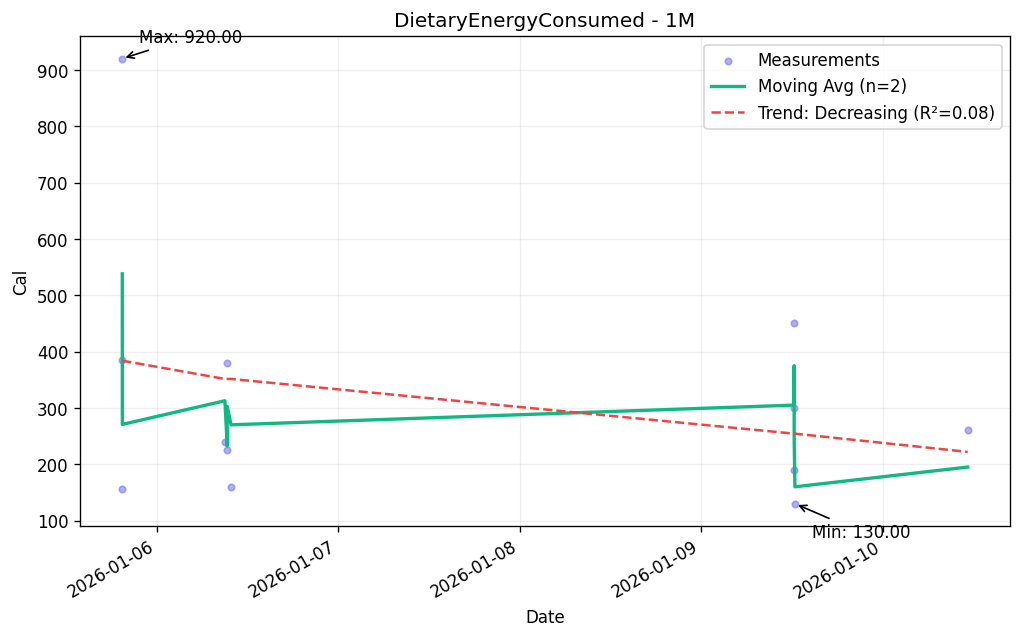
\includegraphics[width=0.95\textwidth]{plots_medical/Nutrition/dietaryenergyconsumed_1M.png}
\end{figure}
\begin{figure}[H]
\centering
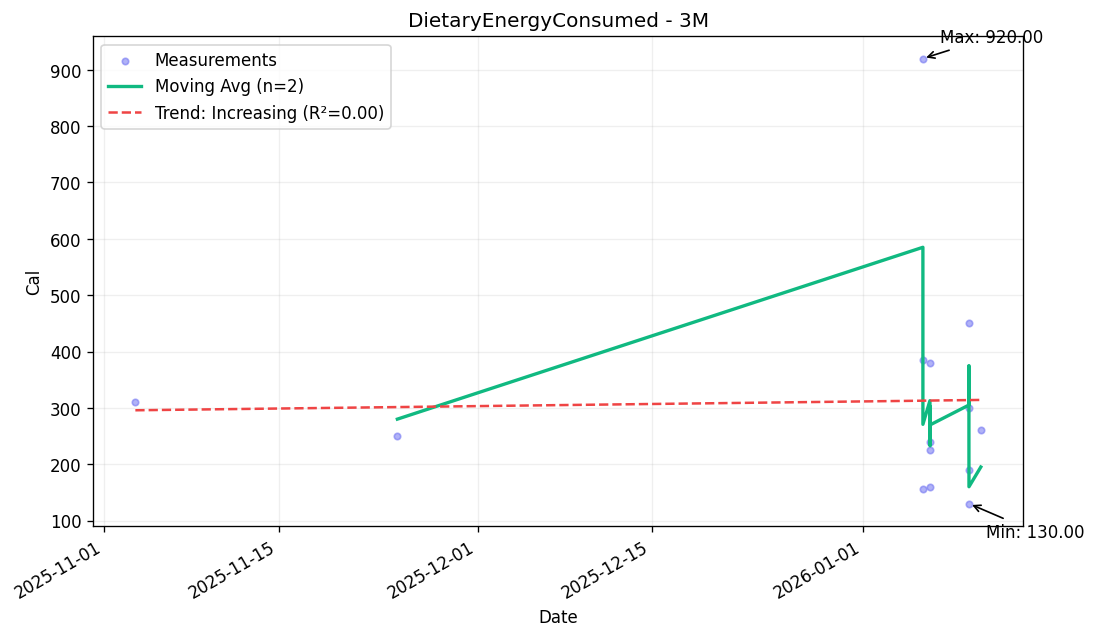
\includegraphics[width=0.95\textwidth]{plots_medical/Nutrition/dietaryenergyconsumed_3M.png}
\end{figure}
\begin{figure}[H]
\centering
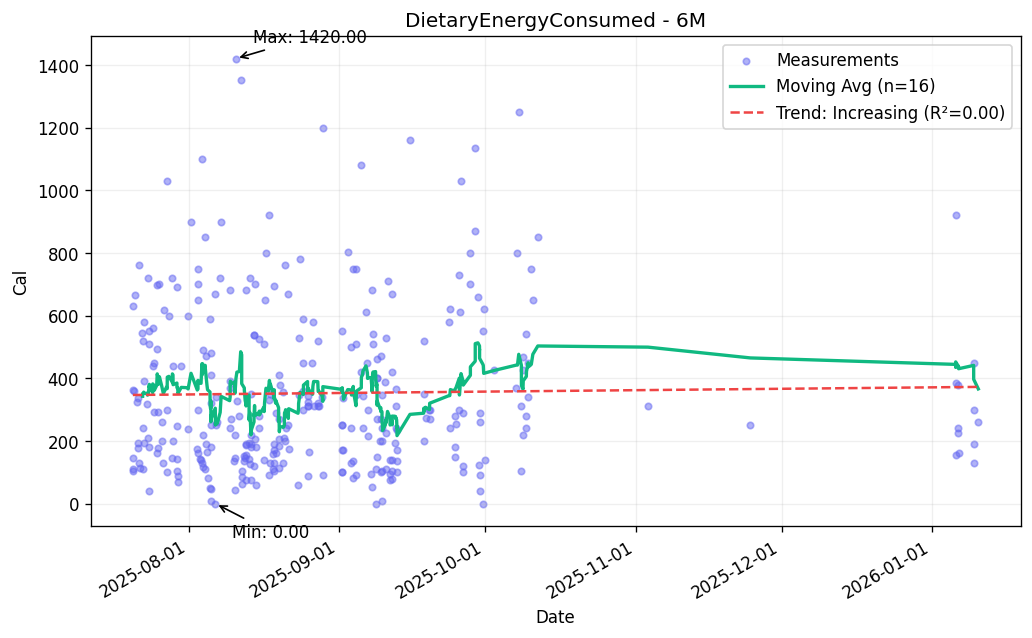
\includegraphics[width=0.95\textwidth]{plots_medical/Nutrition/dietaryenergyconsumed_6M.png}
\end{figure}
\begin{figure}[H]
\centering
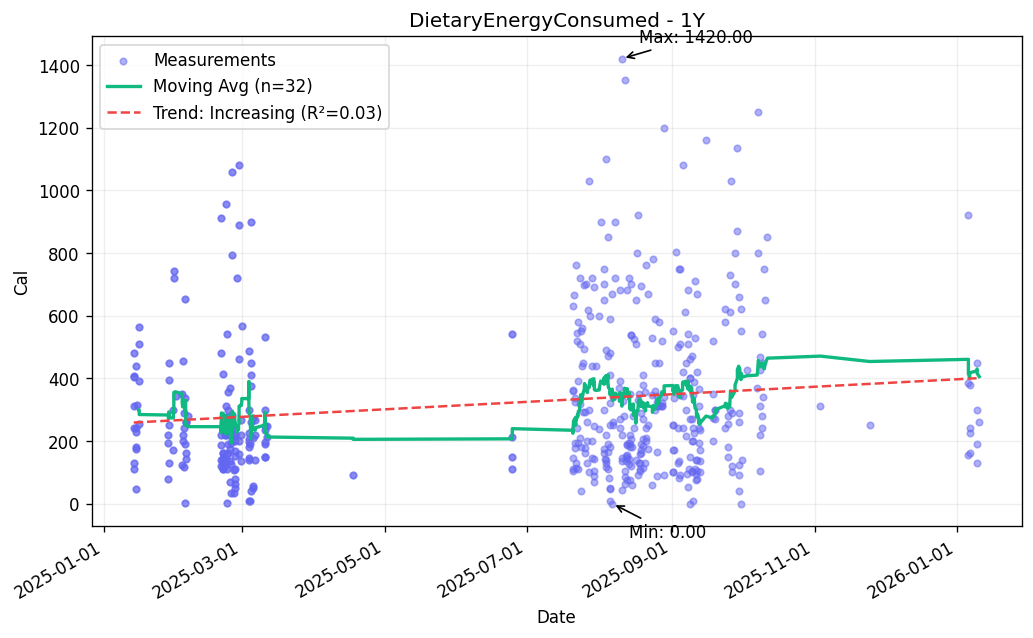
\includegraphics[width=0.95\textwidth]{plots_medical/Nutrition/dietaryenergyconsumed_1Y.png}
\end{figure}
\begin{figure}[H]
\centering
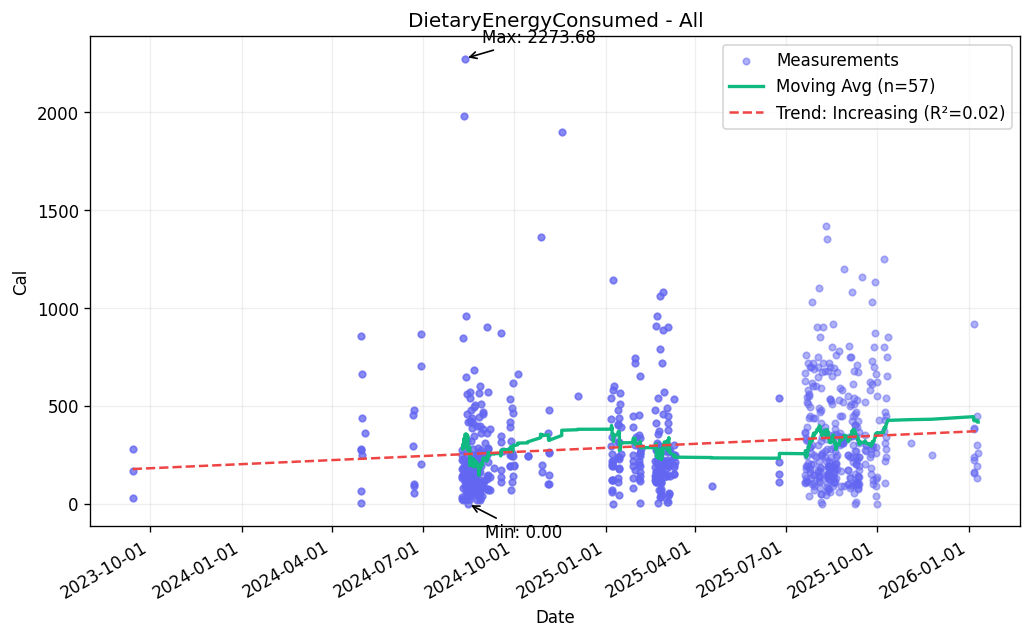
\includegraphics[width=0.95\textwidth]{plots_medical/Nutrition/dietaryenergyconsumed_All.png}
\end{figure}
\clearpage
\subsection{DietaryFatTotal}
\begin{table}[H]
\centering
\resizebox{\textwidth}{!}{
\begin{tabular}{|l|c|c|c|c|c|c|}
\hline
\textbf{Window} & \textbf{Min} & \textbf{Max} & \textbf{Avg} & \textbf{Start} & \textbf{End} & \textbf{Trend Slope} \\ \hline
1W & 0.00 g & 32.00 g & 12.08 g & 32.00 & 21.00 & 0.26680 \\ \hline
1M & 0.00 g & 32.00 g & 12.08 g & 32.00 & 21.00 & 0.26680 \\ \hline
3M & 0.00 g & 32.00 g & 11.36 g & 3.00 & 21.00 & 0.10627 \\ \hline
6M & 0.00 g & 76.00 g & 12.10 g & 0.00 & 21.00 & 0.02254 \\ \hline
1Y & 0.00 g & 76.00 g & 12.11 g & 13.00 & 21.00 & 0.00158 \\ \hline
All & 0.00 g & 113.68 g & 10.70 g & 1.69 & 21.00 & 0.00991 \\ \hline
\end{tabular}
}
\caption{Detailed Statistics for DietaryFatTotal}
\end{table}
\begin{figure}[H]
\centering
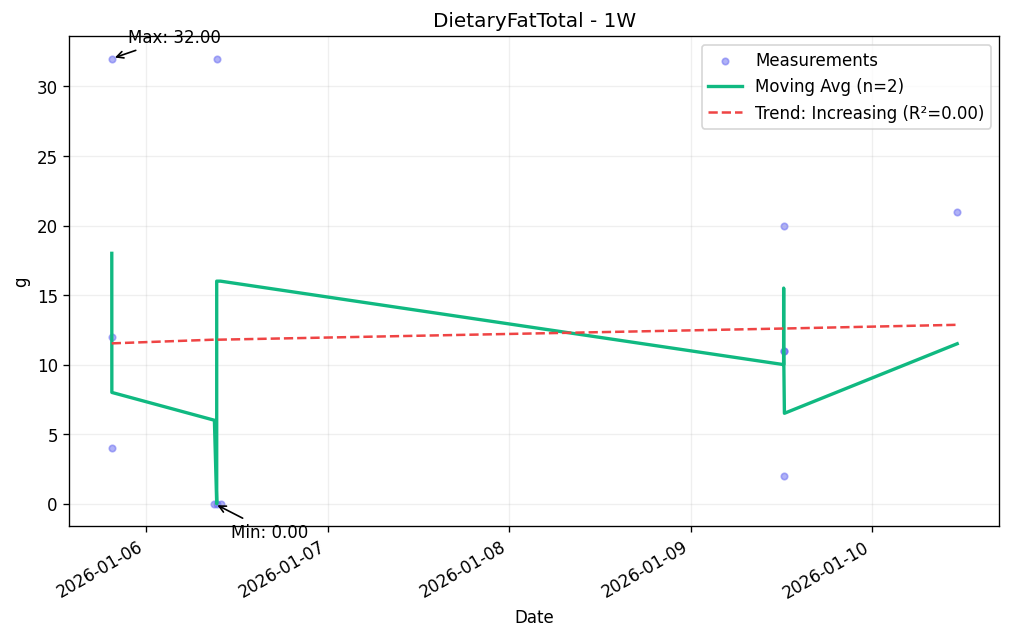
\includegraphics[width=0.95\textwidth]{plots_medical/Nutrition/dietaryfattotal_1W.png}
\end{figure}
\begin{figure}[H]
\centering
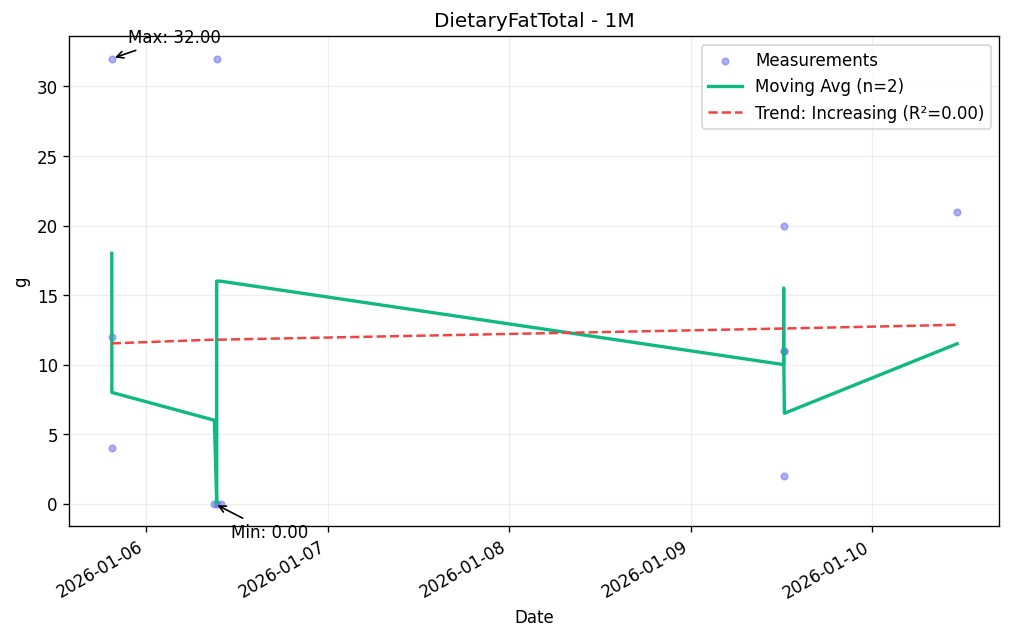
\includegraphics[width=0.95\textwidth]{plots_medical/Nutrition/dietaryfattotal_1M.png}
\end{figure}
\begin{figure}[H]
\centering
\includegraphics[width=0.95\textwidth]{plots_medical/Nutrition/dietaryfattotal_3M.png}
\end{figure}
\begin{figure}[H]
\centering
\includegraphics[width=0.95\textwidth]{plots_medical/Nutrition/dietaryfattotal_6M.png}
\end{figure}
\begin{figure}[H]
\centering
\includegraphics[width=0.95\textwidth]{plots_medical/Nutrition/dietaryfattotal_1Y.png}
\end{figure}
\begin{figure}[H]
\centering
\includegraphics[width=0.95\textwidth]{plots_medical/Nutrition/dietaryfattotal_All.png}
\end{figure}
\clearpage
\subsection{DietaryProtein}
\begin{table}[H]
\centering
\resizebox{\textwidth}{!}{
\begin{tabular}{|l|c|c|c|c|c|c|}
\hline
\textbf{Window} & \textbf{Min} & \textbf{Max} & \textbf{Avg} & \textbf{Start} & \textbf{End} & \textbf{Trend Slope} \\ \hline
1W & 0.00 g & 48.00 g & 13.29 g & 48.00 & 16.00 & -0.81365 \\ \hline
1M & 0.00 g & 48.00 g & 13.29 g & 48.00 & 16.00 & -0.81365 \\ \hline
3M & 0.00 g & 48.00 g & 13.46 g & 13.00 & 16.00 & -0.02139 \\ \hline
6M & 0.00 g & 104.00 g & 13.60 g & 1.00 & 16.00 & 0.03199 \\ \hline
1Y & 0.00 g & 104.00 g & 12.12 g & 9.75 & 16.00 & 0.01527 \\ \hline
All & 0.00 g & 104.00 g & 10.83 g & 5.28 & 16.00 & 0.01232 \\ \hline
\end{tabular}
}
\caption{Detailed Statistics for DietaryProtein}
\end{table}
\begin{figure}[H]
\centering
\includegraphics[width=0.95\textwidth]{plots_medical/Nutrition/dietaryprotein_1W.png}
\end{figure}
\begin{figure}[H]
\centering
\includegraphics[width=0.95\textwidth]{plots_medical/Nutrition/dietaryprotein_1M.png}
\end{figure}
\begin{figure}[H]
\centering
\includegraphics[width=0.95\textwidth]{plots_medical/Nutrition/dietaryprotein_3M.png}
\end{figure}
\begin{figure}[H]
\centering
\includegraphics[width=0.95\textwidth]{plots_medical/Nutrition/dietaryprotein_6M.png}
\end{figure}
\begin{figure}[H]
\centering
\includegraphics[width=0.95\textwidth]{plots_medical/Nutrition/dietaryprotein_1Y.png}
\end{figure}
\begin{figure}[H]
\centering
\includegraphics[width=0.95\textwidth]{plots_medical/Nutrition/dietaryprotein_All.png}
\end{figure}
\clearpage
\subsection{DietaryWater}
\begin{table}[H]
\centering
\resizebox{\textwidth}{!}{
\begin{tabular}{|l|c|c|c|c|c|c|}
\hline
\textbf{Window} & \textbf{Min} & \textbf{Max} & \textbf{Avg} & \textbf{Start} & \textbf{End} & \textbf{Trend Slope} \\ \hline
1W & - & - & - & - & - & - \\ \hline
1M & - & - & - & - & - & - \\ \hline
3M & - & - & - & - & - & - \\ \hline
6M & 31.96 mL & 2957.35 mL & 1007.09 mL & 31.96 & 2957.35 & 17.41306 \\ \hline
1Y & 4.21 mL & 2957.35 mL & 156.46 mL & 36.80 & 2957.35 & 3.74919 \\ \hline
All & 0.73 mL & 2957.35 mL & 139.05 mL & 195.52 & 2957.35 & 0.42196 \\ \hline
\end{tabular}
}
\caption{Detailed Statistics for DietaryWater}
\end{table}
\begin{figure}[H]
\centering
\includegraphics[width=0.95\textwidth]{plots_medical/Nutrition/dietarywater_1W.png}
\end{figure}
\begin{figure}[H]
\centering
\includegraphics[width=0.95\textwidth]{plots_medical/Nutrition/dietarywater_1M.png}
\end{figure}
\begin{figure}[H]
\centering
\includegraphics[width=0.95\textwidth]{plots_medical/Nutrition/dietarywater_3M.png}
\end{figure}
\begin{figure}[H]
\centering
\includegraphics[width=0.95\textwidth]{plots_medical/Nutrition/dietarywater_6M.png}
\end{figure}
\begin{figure}[H]
\centering
\includegraphics[width=0.95\textwidth]{plots_medical/Nutrition/dietarywater_1Y.png}
\end{figure}
\begin{figure}[H]
\centering
\includegraphics[width=0.95\textwidth]{plots_medical/Nutrition/dietarywater_All.png}
\end{figure}
\clearpage
\section{Audio \& Environmental}
\subsection{EnvironmentalAudioExposure}
\begin{table}[H]
\centering
\resizebox{\textwidth}{!}{
\begin{tabular}{|l|c|c|c|c|c|c|}
\hline
\textbf{Window} & \textbf{Min} & \textbf{Max} & \textbf{Avg} & \textbf{Start} & \textbf{End} & \textbf{Trend Slope} \\ \hline
1W & 33.15 dBASPL & 79.39 dBASPL & 58.60 dBASPL & 61.30 & 48.26 & 0.60645 \\ \hline
1M & 33.00 dBASPL & 90.90 dBASPL & 58.22 dBASPL & 75.89 & 48.26 & 0.00987 \\ \hline
3M & 32.92 dBASPL & 99.99 dBASPL & 59.46 dBASPL & 72.13 & 48.26 & -0.03019 \\ \hline
6M & 32.92 dBASPL & 99.99 dBASPL & 59.25 dBASPL & 49.81 & 48.26 & 0.00223 \\ \hline
1Y & 32.92 dBASPL & 99.99 dBASPL & 59.11 dBASPL & 48.75 & 48.26 & 0.00231 \\ \hline
All & 32.67 dBASPL & 101.21 dBASPL & 59.53 dBASPL & 59.18 & 48.26 & -0.00333 \\ \hline
\end{tabular}
}
\caption{Detailed Statistics for EnvironmentalAudioExposure}
\end{table}
\begin{figure}[H]
\centering
\includegraphics[width=0.95\textwidth]{plots_medical/Audio_and_Environmental/environmentalaudioexposure_1W.png}
\end{figure}
\begin{figure}[H]
\centering
\includegraphics[width=0.95\textwidth]{plots_medical/Audio_and_Environmental/environmentalaudioexposure_1M.png}
\end{figure}
\begin{figure}[H]
\centering
\includegraphics[width=0.95\textwidth]{plots_medical/Audio_and_Environmental/environmentalaudioexposure_3M.png}
\end{figure}
\begin{figure}[H]
\centering
\includegraphics[width=0.95\textwidth]{plots_medical/Audio_and_Environmental/environmentalaudioexposure_6M.png}
\end{figure}
\begin{figure}[H]
\centering
\includegraphics[width=0.95\textwidth]{plots_medical/Audio_and_Environmental/environmentalaudioexposure_1Y.png}
\end{figure}
\begin{figure}[H]
\centering
\includegraphics[width=0.95\textwidth]{plots_medical/Audio_and_Environmental/environmentalaudioexposure_All.png}
\end{figure}
\clearpage
\subsection{HeadphoneAudioExposure}
\begin{table}[H]
\centering
\resizebox{\textwidth}{!}{
\begin{tabular}{|l|c|c|c|c|c|c|}
\hline
\textbf{Window} & \textbf{Min} & \textbf{Max} & \textbf{Avg} & \textbf{Start} & \textbf{End} & \textbf{Trend Slope} \\ \hline
1W & 8.01 dBASPL & 97.14 dBASPL & 71.98 dBASPL & 70.17 & 74.18 & -1.03857 \\ \hline
1M & 8.01 dBASPL & 106.95 dBASPL & 75.12 dBASPL & 85.69 & 74.18 & -0.38942 \\ \hline
3M & 0.22 dBASPL & 106.95 dBASPL & 76.75 dBASPL & 83.79 & 74.18 & -0.00527 \\ \hline
6M & 0.03 dBASPL & 106.95 dBASPL & 79.23 dBASPL & 65.39 & 74.18 & -0.05153 \\ \hline
1Y & 0.01 dBASPL & 106.95 dBASPL & 76.32 dBASPL & 75.45 & 74.18 & 0.01928 \\ \hline
All & 0.00 dBASPL & 106.95 dBASPL & 71.86 dBASPL & 84.59 & 74.18 & 0.00881 \\ \hline
\end{tabular}
}
\caption{Detailed Statistics for HeadphoneAudioExposure}
\end{table}
\begin{figure}[H]
\centering
\includegraphics[width=0.95\textwidth]{plots_medical/Audio_and_Environmental/headphoneaudioexposure_1W.png}
\end{figure}
\begin{figure}[H]
\centering
\includegraphics[width=0.95\textwidth]{plots_medical/Audio_and_Environmental/headphoneaudioexposure_1M.png}
\end{figure}
\begin{figure}[H]
\centering
\includegraphics[width=0.95\textwidth]{plots_medical/Audio_and_Environmental/headphoneaudioexposure_3M.png}
\end{figure}
\begin{figure}[H]
\centering
\includegraphics[width=0.95\textwidth]{plots_medical/Audio_and_Environmental/headphoneaudioexposure_6M.png}
\end{figure}
\begin{figure}[H]
\centering
\includegraphics[width=0.95\textwidth]{plots_medical/Audio_and_Environmental/headphoneaudioexposure_1Y.png}
\end{figure}
\begin{figure}[H]
\centering
\includegraphics[width=0.95\textwidth]{plots_medical/Audio_and_Environmental/headphoneaudioexposure_All.png}
\end{figure}
\clearpage
\subsection{TimeInDaylight}
\begin{table}[H]
\centering
\resizebox{\textwidth}{!}{
\begin{tabular}{|l|c|c|c|c|c|c|}
\hline
\textbf{Window} & \textbf{Min} & \textbf{Max} & \textbf{Avg} & \textbf{Start} & \textbf{End} & \textbf{Trend Slope} \\ \hline
1W & 1.00 min & 5.00 min & 4.44 min & 5.00 & 1.00 & -0.03134 \\ \hline
1M & 1.00 min & 5.00 min & 4.25 min & 5.00 & 1.00 & 0.04029 \\ \hline
3M & 1.00 min & 5.00 min & 4.22 min & 3.00 & 1.00 & 0.00092 \\ \hline
6M & 1.00 min & 5.00 min & 4.02 min & 1.00 & 1.00 & 0.00649 \\ \hline
1Y & 1.00 min & 5.00 min & 4.30 min & 5.00 & 1.00 & -0.00131 \\ \hline
All & 1.00 min & 5.00 min & 4.28 min & 3.00 & 1.00 & -0.00012 \\ \hline
\end{tabular}
}
\caption{Detailed Statistics for TimeInDaylight}
\end{table}
\begin{figure}[H]
\centering
\includegraphics[width=0.95\textwidth]{plots_medical/Audio_and_Environmental/timeindaylight_1W.png}
\end{figure}
\begin{figure}[H]
\centering
\includegraphics[width=0.95\textwidth]{plots_medical/Audio_and_Environmental/timeindaylight_1M.png}
\end{figure}
\begin{figure}[H]
\centering
\includegraphics[width=0.95\textwidth]{plots_medical/Audio_and_Environmental/timeindaylight_3M.png}
\end{figure}
\begin{figure}[H]
\centering
\includegraphics[width=0.95\textwidth]{plots_medical/Audio_and_Environmental/timeindaylight_6M.png}
\end{figure}
\begin{figure}[H]
\centering
\includegraphics[width=0.95\textwidth]{plots_medical/Audio_and_Environmental/timeindaylight_1Y.png}
\end{figure}
\begin{figure}[H]
\centering
\includegraphics[width=0.95\textwidth]{plots_medical/Audio_and_Environmental/timeindaylight_All.png}
\end{figure}
\clearpage
\subsection{UnderwaterDepth}
\begin{table}[H]
\centering
\resizebox{\textwidth}{!}{
\begin{tabular}{|l|c|c|c|c|c|c|}
\hline
\textbf{Window} & \textbf{Min} & \textbf{Max} & \textbf{Avg} & \textbf{Start} & \textbf{End} & \textbf{Trend Slope} \\ \hline
1W & - & - & - & - & - & - \\ \hline
1M & 3.56 ft & 12.25 ft & 7.82 ft & 5.44 & 7.73 & -0.04345 \\ \hline
3M & 3.32 ft & 12.25 ft & 6.78 ft & 3.33 & 7.73 & 0.04367 \\ \hline
6M & 3.28 ft & 12.25 ft & 4.77 ft & 3.63 & 7.73 & 0.03120 \\ \hline
1Y & 3.28 ft & 12.25 ft & 4.77 ft & 3.63 & 7.73 & 0.03120 \\ \hline
All & 3.28 ft & 12.25 ft & 4.77 ft & 3.63 & 7.73 & 0.03120 \\ \hline
\end{tabular}
}
\caption{Detailed Statistics for UnderwaterDepth}
\end{table}
\begin{figure}[H]
\centering
\includegraphics[width=0.95\textwidth]{plots_medical/Audio_and_Environmental/underwaterdepth_1W.png}
\end{figure}
\begin{figure}[H]
\centering
\includegraphics[width=0.95\textwidth]{plots_medical/Audio_and_Environmental/underwaterdepth_1M.png}
\end{figure}
\begin{figure}[H]
\centering
\includegraphics[width=0.95\textwidth]{plots_medical/Audio_and_Environmental/underwaterdepth_3M.png}
\end{figure}
\begin{figure}[H]
\centering
\includegraphics[width=0.95\textwidth]{plots_medical/Audio_and_Environmental/underwaterdepth_6M.png}
\end{figure}
\begin{figure}[H]
\centering
\includegraphics[width=0.95\textwidth]{plots_medical/Audio_and_Environmental/underwaterdepth_1Y.png}
\end{figure}
\begin{figure}[H]
\centering
\includegraphics[width=0.95\textwidth]{plots_medical/Audio_and_Environmental/underwaterdepth_All.png}
\end{figure}
\clearpage
\subsection{WaterTemperature}
\begin{table}[H]
\centering
\resizebox{\textwidth}{!}{
\begin{tabular}{|l|c|c|c|c|c|c|}
\hline
\textbf{Window} & \textbf{Min} & \textbf{Max} & \textbf{Avg} & \textbf{Start} & \textbf{End} & \textbf{Trend Slope} \\ \hline
1W & - & - & - & - & - & - \\ \hline
1M & 80.40 degF & 100.09 degF & 85.38 degF & 83.28 & 98.62 & 0.14452 \\ \hline
3M & 76.12 degF & 101.26 degF & 82.78 degF & 81.95 & 98.62 & 0.13071 \\ \hline
6M & 76.12 degF & 101.26 degF & 82.89 degF & 81.45 & 98.62 & 0.02001 \\ \hline
1Y & 76.12 degF & 101.26 degF & 82.89 degF & 81.45 & 98.62 & 0.02001 \\ \hline
All & 76.12 degF & 101.26 degF & 82.89 degF & 81.45 & 98.62 & 0.02001 \\ \hline
\end{tabular}
}
\caption{Detailed Statistics for WaterTemperature}
\end{table}
\begin{figure}[H]
\centering
\includegraphics[width=0.95\textwidth]{plots_medical/Audio_and_Environmental/watertemperature_1W.png}
\end{figure}
\begin{figure}[H]
\centering
\includegraphics[width=0.95\textwidth]{plots_medical/Audio_and_Environmental/watertemperature_1M.png}
\end{figure}
\begin{figure}[H]
\centering
\includegraphics[width=0.95\textwidth]{plots_medical/Audio_and_Environmental/watertemperature_3M.png}
\end{figure}
\begin{figure}[H]
\centering
\includegraphics[width=0.95\textwidth]{plots_medical/Audio_and_Environmental/watertemperature_6M.png}
\end{figure}
\begin{figure}[H]
\centering
\includegraphics[width=0.95\textwidth]{plots_medical/Audio_and_Environmental/watertemperature_1Y.png}
\end{figure}
\begin{figure}[H]
\centering
\includegraphics[width=0.95\textwidth]{plots_medical/Audio_and_Environmental/watertemperature_All.png}
\end{figure}
\clearpage
\section{Other}
\subsection{AppleSleepingBreathingDisturbances}
\begin{table}[H]
\centering
\resizebox{\textwidth}{!}{
\begin{tabular}{|l|c|c|c|c|c|c|}
\hline
\textbf{Window} & \textbf{Min} & \textbf{Max} & \textbf{Avg} & \textbf{Start} & \textbf{End} & \textbf{Trend Slope} \\ \hline
1W & 0.38 count & 3.28 count & 1.79 count & 2.32 & 2.45 & 0.00409 \\ \hline
1M & 0.00 count & 3.28 count & 1.13 count & 0.21 & 2.45 & 0.04752 \\ \hline
3M & 0.00 count & 4.61 count & 1.36 count & 0.15 & 2.45 & 0.00132 \\ \hline
6M & 0.00 count & 5.10 count & 1.45 count & 1.23 & 2.45 & -0.00180 \\ \hline
1Y & 0.00 count & 5.25 count & 1.51 count & 2.57 & 2.45 & -0.00056 \\ \hline
All & 0.00 count & 5.25 count & 1.55 count & 1.23 & 2.45 & -0.00078 \\ \hline
\end{tabular}
}
\caption{Detailed Statistics for AppleSleepingBreathingDisturbances}
\end{table}
\begin{figure}[H]
\centering
\includegraphics[width=0.95\textwidth]{plots_medical/Other/applesleepingbreathingdisturbances_1W.png}
\end{figure}
\begin{figure}[H]
\centering
\includegraphics[width=0.95\textwidth]{plots_medical/Other/applesleepingbreathingdisturbances_1M.png}
\end{figure}
\begin{figure}[H]
\centering
\includegraphics[width=0.95\textwidth]{plots_medical/Other/applesleepingbreathingdisturbances_3M.png}
\end{figure}
\begin{figure}[H]
\centering
\includegraphics[width=0.95\textwidth]{plots_medical/Other/applesleepingbreathingdisturbances_6M.png}
\end{figure}
\begin{figure}[H]
\centering
\includegraphics[width=0.95\textwidth]{plots_medical/Other/applesleepingbreathingdisturbances_1Y.png}
\end{figure}
\begin{figure}[H]
\centering
\includegraphics[width=0.95\textwidth]{plots_medical/Other/applesleepingbreathingdisturbances_All.png}
\end{figure}
\clearpage
\subsection{AppleSleepingWristTemperature}
\begin{table}[H]
\centering
\resizebox{\textwidth}{!}{
\begin{tabular}{|l|c|c|c|c|c|c|}
\hline
\textbf{Window} & \textbf{Min} & \textbf{Max} & \textbf{Avg} & \textbf{Start} & \textbf{End} & \textbf{Trend Slope} \\ \hline
1W & 94.74 degF & 96.46 degF & 95.57 degF & 95.07 & 96.46 & 0.16983 \\ \hline
1M & 94.74 degF & 96.54 degF & 95.69 degF & 95.26 & 96.46 & 0.01219 \\ \hline
3M & 93.57 degF & 100.03 degF & 96.08 degF & 96.40 & 96.46 & -0.00160 \\ \hline
6M & 93.55 degF & 100.03 degF & 95.77 degF & 96.16 & 96.46 & 0.00306 \\ \hline
1Y & 93.55 degF & 100.03 degF & 95.74 degF & 96.26 & 96.46 & 0.00081 \\ \hline
All & 93.55 degF & 100.03 degF & 95.84 degF & 95.60 & 96.46 & -0.00063 \\ \hline
\end{tabular}
}
\caption{Detailed Statistics for AppleSleepingWristTemperature}
\end{table}
\begin{figure}[H]
\centering
\includegraphics[width=0.95\textwidth]{plots_medical/Other/applesleepingwristtemperature_1W.png}
\end{figure}
\begin{figure}[H]
\centering
\includegraphics[width=0.95\textwidth]{plots_medical/Other/applesleepingwristtemperature_1M.png}
\end{figure}
\begin{figure}[H]
\centering
\includegraphics[width=0.95\textwidth]{plots_medical/Other/applesleepingwristtemperature_3M.png}
\end{figure}
\begin{figure}[H]
\centering
\includegraphics[width=0.95\textwidth]{plots_medical/Other/applesleepingwristtemperature_6M.png}
\end{figure}
\begin{figure}[H]
\centering
\includegraphics[width=0.95\textwidth]{plots_medical/Other/applesleepingwristtemperature_1Y.png}
\end{figure}
\begin{figure}[H]
\centering
\includegraphics[width=0.95\textwidth]{plots_medical/Other/applesleepingwristtemperature_All.png}
\end{figure}
\clearpage
\subsection{AppleStandTime}
\begin{table}[H]
\centering
\resizebox{\textwidth}{!}{
\begin{tabular}{|l|c|c|c|c|c|c|}
\hline
\textbf{Window} & \textbf{Min} & \textbf{Max} & \textbf{Avg} & \textbf{Start} & \textbf{End} & \textbf{Trend Slope} \\ \hline
1W & 1.00 min & 5.00 min & 2.40 min & 1.00 & 3.00 & 0.11161 \\ \hline
1M & 1.00 min & 5.00 min & 2.11 min & 1.00 & 3.00 & 0.02512 \\ \hline
3M & 1.00 min & 5.00 min & 2.45 min & 1.00 & 3.00 & -0.00659 \\ \hline
6M & 1.00 min & 5.00 min & 2.56 min & 2.00 & 3.00 & -0.00202 \\ \hline
1Y & 1.00 min & 5.00 min & 2.62 min & 1.00 & 3.00 & -0.00087 \\ \hline
All & 1.00 min & 5.00 min & 2.56 min & 1.00 & 3.00 & -0.00003 \\ \hline
\end{tabular}
}
\caption{Detailed Statistics for AppleStandTime}
\end{table}
\begin{figure}[H]
\centering
\includegraphics[width=0.95\textwidth]{plots_medical/Other/applestandtime_1W.png}
\end{figure}
\begin{figure}[H]
\centering
\includegraphics[width=0.95\textwidth]{plots_medical/Other/applestandtime_1M.png}
\end{figure}
\begin{figure}[H]
\centering
\includegraphics[width=0.95\textwidth]{plots_medical/Other/applestandtime_3M.png}
\end{figure}
\begin{figure}[H]
\centering
\includegraphics[width=0.95\textwidth]{plots_medical/Other/applestandtime_6M.png}
\end{figure}
\begin{figure}[H]
\centering
\includegraphics[width=0.95\textwidth]{plots_medical/Other/applestandtime_1Y.png}
\end{figure}
\begin{figure}[H]
\centering
\includegraphics[width=0.95\textwidth]{plots_medical/Other/applestandtime_All.png}
\end{figure}
\clearpage
\subsection{AppleWalkingSteadiness}
\begin{table}[H]
\centering
\resizebox{\textwidth}{!}{
\begin{tabular}{|l|c|c|c|c|c|c|}
\hline
\textbf{Window} & \textbf{Min} & \textbf{Max} & \textbf{Avg} & \textbf{Start} & \textbf{End} & \textbf{Trend Slope} \\ \hline
1W & 0.99 \% & 0.99 \% & 0.99 \% & 0.99 & 0.99 & -0.00061 \\ \hline
1M & 0.99 \% & 1.00 \% & 1.00 \% & 1.00 & 0.99 & -0.00040 \\ \hline
3M & 0.95 \% & 1.00 \% & 0.98 \% & 0.96 & 0.99 & 0.00038 \\ \hline
6M & 0.92 \% & 1.00 \% & 0.97 \% & 0.96 & 0.99 & 0.00020 \\ \hline
1Y & 0.92 \% & 1.00 \% & 0.97 \% & 0.99 & 0.99 & 0.00005 \\ \hline
All & 0.92 \% & 1.00 \% & 0.97 \% & 0.95 & 0.99 & 0.00000 \\ \hline
\end{tabular}
}
\caption{Detailed Statistics for AppleWalkingSteadiness}
\end{table}
\begin{figure}[H]
\centering
\includegraphics[width=0.95\textwidth]{plots_medical/Other/applewalkingsteadiness_1W.png}
\end{figure}
\begin{figure}[H]
\centering
\includegraphics[width=0.95\textwidth]{plots_medical/Other/applewalkingsteadiness_1M.png}
\end{figure}
\begin{figure}[H]
\centering
\includegraphics[width=0.95\textwidth]{plots_medical/Other/applewalkingsteadiness_3M.png}
\end{figure}
\begin{figure}[H]
\centering
\includegraphics[width=0.95\textwidth]{plots_medical/Other/applewalkingsteadiness_6M.png}
\end{figure}
\begin{figure}[H]
\centering
\includegraphics[width=0.95\textwidth]{plots_medical/Other/applewalkingsteadiness_1Y.png}
\end{figure}
\begin{figure}[H]
\centering
\includegraphics[width=0.95\textwidth]{plots_medical/Other/applewalkingsteadiness_All.png}
\end{figure}
\clearpage
\subsection{BasalEnergyBurned}
\begin{table}[H]
\centering
\resizebox{\textwidth}{!}{
\begin{tabular}{|l|c|c|c|c|c|c|}
\hline
\textbf{Window} & \textbf{Min} & \textbf{Max} & \textbf{Avg} & \textbf{Start} & \textbf{End} & \textbf{Trend Slope} \\ \hline
1W & 0.08 Cal & 1851.00 Cal & 5.56 Cal & 1.00 & 23.11 & -1.39693 \\ \hline
1M & 0.08 Cal & 1851.00 Cal & 5.80 Cal & 25.29 & 23.11 & -0.22910 \\ \hline
3M & 0.06 Cal & 1851.00 Cal & 4.11 Cal & 0.55 & 23.11 & 0.03301 \\ \hline
6M & 0.06 Cal & 1897.00 Cal & 4.71 Cal & 0.59 & 23.11 & -0.04034 \\ \hline
1Y & 0.06 Cal & 1904.00 Cal & 6.50 Cal & 22.89 & 23.11 & -0.03343 \\ \hline
All & 0.05 Cal & 1904.00 Cal & 8.32 Cal & 19.54 & 23.11 & -0.01196 \\ \hline
\end{tabular}
}
\caption{Detailed Statistics for BasalEnergyBurned}
\end{table}
\begin{figure}[H]
\centering
\includegraphics[width=0.95\textwidth]{plots_medical/Other/basalenergyburned_1W.png}
\end{figure}
\begin{figure}[H]
\centering
\includegraphics[width=0.95\textwidth]{plots_medical/Other/basalenergyburned_1M.png}
\end{figure}
\begin{figure}[H]
\centering
\includegraphics[width=0.95\textwidth]{plots_medical/Other/basalenergyburned_3M.png}
\end{figure}
\begin{figure}[H]
\centering
\includegraphics[width=0.95\textwidth]{plots_medical/Other/basalenergyburned_6M.png}
\end{figure}
\begin{figure}[H]
\centering
\includegraphics[width=0.95\textwidth]{plots_medical/Other/basalenergyburned_1Y.png}
\end{figure}
\begin{figure}[H]
\centering
\includegraphics[width=0.95\textwidth]{plots_medical/Other/basalenergyburned_All.png}
\end{figure}
\clearpage
\subsection{DietaryCalcium}
\begin{table}[H]
\centering
\resizebox{\textwidth}{!}{
\begin{tabular}{|l|c|c|c|c|c|c|}
\hline
\textbf{Window} & \textbf{Min} & \textbf{Max} & \textbf{Avg} & \textbf{Start} & \textbf{End} & \textbf{Trend Slope} \\ \hline
1W & - & - & - & - & - & - \\ \hline
1M & - & - & - & - & - & - \\ \hline
3M & 28.52 mg & 112.00 mg & 66.84 mg & 28.52 & 112.00 & 0.84529 \\ \hline
6M & 0.00 mg & 541.02 mg & 63.03 mg & 50.00 & 112.00 & 0.22648 \\ \hline
1Y & 0.00 mg & 942.86 mg & 55.00 mg & 54.00 & 112.00 & 0.08372 \\ \hline
All & 0.00 mg & 942.86 mg & 55.70 mg & 30.94 & 112.00 & 0.05166 \\ \hline
\end{tabular}
}
\caption{Detailed Statistics for DietaryCalcium}
\end{table}
\begin{figure}[H]
\centering
\includegraphics[width=0.95\textwidth]{plots_medical/Other/dietarycalcium_1W.png}
\end{figure}
\begin{figure}[H]
\centering
\includegraphics[width=0.95\textwidth]{plots_medical/Other/dietarycalcium_1M.png}
\end{figure}
\begin{figure}[H]
\centering
\includegraphics[width=0.95\textwidth]{plots_medical/Other/dietarycalcium_3M.png}
\end{figure}
\begin{figure}[H]
\centering
\includegraphics[width=0.95\textwidth]{plots_medical/Other/dietarycalcium_6M.png}
\end{figure}
\begin{figure}[H]
\centering
\includegraphics[width=0.95\textwidth]{plots_medical/Other/dietarycalcium_1Y.png}
\end{figure}
\begin{figure}[H]
\centering
\includegraphics[width=0.95\textwidth]{plots_medical/Other/dietarycalcium_All.png}
\end{figure}
\clearpage
\subsection{DietaryCholesterol}
\begin{table}[H]
\centering
\resizebox{\textwidth}{!}{
\begin{tabular}{|l|c|c|c|c|c|c|}
\hline
\textbf{Window} & \textbf{Min} & \textbf{Max} & \textbf{Avg} & \textbf{Start} & \textbf{End} & \textbf{Trend Slope} \\ \hline
1W & 20.00 mg & 451.24 mg & 240.06 mg & 100.00 & 451.24 & 52.29907 \\ \hline
1M & 20.00 mg & 451.24 mg & 240.06 mg & 100.00 & 451.24 & 52.29907 \\ \hline
3M & 5.00 mg & 451.24 mg & 164.21 mg & 5.00 & 451.24 & 4.07462 \\ \hline
6M & 4.00 mg & 768.39 mg & 114.63 mg & 217.00 & 451.24 & 0.40071 \\ \hline
1Y & 0.00 mg & 768.39 mg & 59.09 mg & 0.00 & 451.24 & 0.35884 \\ \hline
All & 0.00 mg & 768.39 mg & 40.89 mg & 14.28 & 451.24 & 0.20065 \\ \hline
\end{tabular}
}
\caption{Detailed Statistics for DietaryCholesterol}
\end{table}
\begin{figure}[H]
\centering
\includegraphics[width=0.95\textwidth]{plots_medical/Other/dietarycholesterol_1W.png}
\end{figure}
\begin{figure}[H]
\centering
\includegraphics[width=0.95\textwidth]{plots_medical/Other/dietarycholesterol_1M.png}
\end{figure}
\begin{figure}[H]
\centering
\includegraphics[width=0.95\textwidth]{plots_medical/Other/dietarycholesterol_3M.png}
\end{figure}
\begin{figure}[H]
\centering
\includegraphics[width=0.95\textwidth]{plots_medical/Other/dietarycholesterol_6M.png}
\end{figure}
\begin{figure}[H]
\centering
\includegraphics[width=0.95\textwidth]{plots_medical/Other/dietarycholesterol_1Y.png}
\end{figure}
\begin{figure}[H]
\centering
\includegraphics[width=0.95\textwidth]{plots_medical/Other/dietarycholesterol_All.png}
\end{figure}
\clearpage
\subsection{DietaryCopper}
\begin{table}[H]
\centering
\resizebox{\textwidth}{!}{
\begin{tabular}{|l|c|c|c|c|c|c|}
\hline
\textbf{Window} & \textbf{Min} & \textbf{Max} & \textbf{Avg} & \textbf{Start} & \textbf{End} & \textbf{Trend Slope} \\ \hline
1W & - & - & - & - & - & - \\ \hline
1M & - & - & - & - & - & - \\ \hline
3M & 0.00 mg & 0.88 mg & 0.17 mg & 0.08 & 0.04 & 0.00012 \\ \hline
6M & 0.00 mg & 0.88 mg & 0.14 mg & 0.08 & 0.04 & 0.00085 \\ \hline
1Y & 0.00 mg & 0.88 mg & 0.11 mg & 0.00 & 0.04 & 0.00031 \\ \hline
All & 0.00 mg & 0.88 mg & 0.11 mg & 0.13 & 0.04 & 0.00024 \\ \hline
\end{tabular}
}
\caption{Detailed Statistics for DietaryCopper}
\end{table}
\begin{figure}[H]
\centering
\includegraphics[width=0.95\textwidth]{plots_medical/Other/dietarycopper_1W.png}
\end{figure}
\begin{figure}[H]
\centering
\includegraphics[width=0.95\textwidth]{plots_medical/Other/dietarycopper_1M.png}
\end{figure}
\begin{figure}[H]
\centering
\includegraphics[width=0.95\textwidth]{plots_medical/Other/dietarycopper_3M.png}
\end{figure}
\begin{figure}[H]
\centering
\includegraphics[width=0.95\textwidth]{plots_medical/Other/dietarycopper_6M.png}
\end{figure}
\begin{figure}[H]
\centering
\includegraphics[width=0.95\textwidth]{plots_medical/Other/dietarycopper_1Y.png}
\end{figure}
\begin{figure}[H]
\centering
\includegraphics[width=0.95\textwidth]{plots_medical/Other/dietarycopper_All.png}
\end{figure}
\clearpage
\subsection{DietaryFatMonounsaturated}
\begin{table}[H]
\centering
\resizebox{\textwidth}{!}{
\begin{tabular}{|l|c|c|c|c|c|c|}
\hline
\textbf{Window} & \textbf{Min} & \textbf{Max} & \textbf{Avg} & \textbf{Start} & \textbf{End} & \textbf{Trend Slope} \\ \hline
1W & - & - & - & - & - & - \\ \hline
1M & - & - & - & - & - & - \\ \hline
3M & 0.00 g & 28.65 g & 1.85 g & 6.05 & 2.84 & 0.04150 \\ \hline
6M & 0.00 g & 28.65 g & 1.76 g & 6.20 & 2.84 & 0.00766 \\ \hline
1Y & 0.00 g & 28.65 g & 1.21 g & 2.95 & 2.84 & 0.00577 \\ \hline
All & 0.00 g & 28.65 g & 1.20 g & 0.26 & 2.84 & 0.00519 \\ \hline
\end{tabular}
}
\caption{Detailed Statistics for DietaryFatMonounsaturated}
\end{table}
\begin{figure}[H]
\centering
\includegraphics[width=0.95\textwidth]{plots_medical/Other/dietaryfatmonounsaturated_1W.png}
\end{figure}
\begin{figure}[H]
\centering
\includegraphics[width=0.95\textwidth]{plots_medical/Other/dietaryfatmonounsaturated_1M.png}
\end{figure}
\begin{figure}[H]
\centering
\includegraphics[width=0.95\textwidth]{plots_medical/Other/dietaryfatmonounsaturated_3M.png}
\end{figure}
\begin{figure}[H]
\centering
\includegraphics[width=0.95\textwidth]{plots_medical/Other/dietaryfatmonounsaturated_6M.png}
\end{figure}
\begin{figure}[H]
\centering
\includegraphics[width=0.95\textwidth]{plots_medical/Other/dietaryfatmonounsaturated_1Y.png}
\end{figure}
\begin{figure}[H]
\centering
\includegraphics[width=0.95\textwidth]{plots_medical/Other/dietaryfatmonounsaturated_All.png}
\end{figure}
\clearpage
\subsection{DietaryFatPolyunsaturated}
\begin{table}[H]
\centering
\resizebox{\textwidth}{!}{
\begin{tabular}{|l|c|c|c|c|c|c|}
\hline
\textbf{Window} & \textbf{Min} & \textbf{Max} & \textbf{Avg} & \textbf{Start} & \textbf{End} & \textbf{Trend Slope} \\ \hline
1W & - & - & - & - & - & - \\ \hline
1M & - & - & - & - & - & - \\ \hline
3M & 0.00 g & 8.59 g & 0.97 g & 3.39 & 1.50 & 0.02944 \\ \hline
6M & 0.00 g & 8.59 g & 1.01 g & 3.47 & 1.50 & 0.00142 \\ \hline
1Y & 0.00 g & 12.14 g & 0.70 g & 0.91 & 1.50 & 0.00298 \\ \hline
All & 0.00 g & 12.14 g & 0.69 g & 0.50 & 1.50 & 0.00266 \\ \hline
\end{tabular}
}
\caption{Detailed Statistics for DietaryFatPolyunsaturated}
\end{table}
\begin{figure}[H]
\centering
\includegraphics[width=0.95\textwidth]{plots_medical/Other/dietaryfatpolyunsaturated_1W.png}
\end{figure}
\begin{figure}[H]
\centering
\includegraphics[width=0.95\textwidth]{plots_medical/Other/dietaryfatpolyunsaturated_1M.png}
\end{figure}
\begin{figure}[H]
\centering
\includegraphics[width=0.95\textwidth]{plots_medical/Other/dietaryfatpolyunsaturated_3M.png}
\end{figure}
\begin{figure}[H]
\centering
\includegraphics[width=0.95\textwidth]{plots_medical/Other/dietaryfatpolyunsaturated_6M.png}
\end{figure}
\begin{figure}[H]
\centering
\includegraphics[width=0.95\textwidth]{plots_medical/Other/dietaryfatpolyunsaturated_1Y.png}
\end{figure}
\begin{figure}[H]
\centering
\includegraphics[width=0.95\textwidth]{plots_medical/Other/dietaryfatpolyunsaturated_All.png}
\end{figure}
\clearpage
\subsection{DietaryFatSaturated}
\begin{table}[H]
\centering
\resizebox{\textwidth}{!}{
\begin{tabular}{|l|c|c|c|c|c|c|}
\hline
\textbf{Window} & \textbf{Min} & \textbf{Max} & \textbf{Avg} & \textbf{Start} & \textbf{End} & \textbf{Trend Slope} \\ \hline
1W & 0.22 g & 20.00 g & 5.69 g & 20.00 & 9.09 & -0.75681 \\ \hline
1M & 0.22 g & 20.00 g & 5.69 g & 20.00 & 9.09 & -0.75681 \\ \hline
3M & 0.22 g & 20.00 g & 4.96 g & 1.50 & 9.09 & 0.05612 \\ \hline
6M & 0.01 g & 20.00 g & 2.90 g & 0.13 & 9.09 & 0.01459 \\ \hline
1Y & 0.00 g & 20.00 g & 3.35 g & 6.50 & 9.09 & -0.00193 \\ \hline
All & 0.00 g & 35.00 g & 3.11 g & 0.40 & 9.09 & 0.00170 \\ \hline
\end{tabular}
}
\caption{Detailed Statistics for DietaryFatSaturated}
\end{table}
\begin{figure}[H]
\centering
\includegraphics[width=0.95\textwidth]{plots_medical/Other/dietaryfatsaturated_1W.png}
\end{figure}
\begin{figure}[H]
\centering
\includegraphics[width=0.95\textwidth]{plots_medical/Other/dietaryfatsaturated_1M.png}
\end{figure}
\begin{figure}[H]
\centering
\includegraphics[width=0.95\textwidth]{plots_medical/Other/dietaryfatsaturated_3M.png}
\end{figure}
\begin{figure}[H]
\centering
\includegraphics[width=0.95\textwidth]{plots_medical/Other/dietaryfatsaturated_6M.png}
\end{figure}
\begin{figure}[H]
\centering
\includegraphics[width=0.95\textwidth]{plots_medical/Other/dietaryfatsaturated_1Y.png}
\end{figure}
\begin{figure}[H]
\centering
\includegraphics[width=0.95\textwidth]{plots_medical/Other/dietaryfatsaturated_All.png}
\end{figure}
\clearpage
\subsection{DietaryFiber}
\begin{table}[H]
\centering
\resizebox{\textwidth}{!}{
\begin{tabular}{|l|c|c|c|c|c|c|}
\hline
\textbf{Window} & \textbf{Min} & \textbf{Max} & \textbf{Avg} & \textbf{Start} & \textbf{End} & \textbf{Trend Slope} \\ \hline
1W & 3.00 g & 11.85 g & 6.74 g & 8.00 & 4.60 & -1.09103 \\ \hline
1M & 3.00 g & 11.85 g & 6.74 g & 8.00 & 4.60 & -1.09103 \\ \hline
3M & 2.00 g & 11.85 g & 6.06 g & 2.00 & 4.60 & 0.06718 \\ \hline
6M & 0.38 g & 20.00 g & 3.18 g & 3.10 & 4.60 & 0.02322 \\ \hline
1Y & 0.00 g & 20.00 g & 3.47 g & 1.62 & 4.60 & -0.00096 \\ \hline
All & 0.00 g & 20.00 g & 3.10 g & 2.14 & 4.60 & 0.00219 \\ \hline
\end{tabular}
}
\caption{Detailed Statistics for DietaryFiber}
\end{table}
\begin{figure}[H]
\centering
\includegraphics[width=0.95\textwidth]{plots_medical/Other/dietaryfiber_1W.png}
\end{figure}
\begin{figure}[H]
\centering
\includegraphics[width=0.95\textwidth]{plots_medical/Other/dietaryfiber_1M.png}
\end{figure}
\begin{figure}[H]
\centering
\includegraphics[width=0.95\textwidth]{plots_medical/Other/dietaryfiber_3M.png}
\end{figure}
\begin{figure}[H]
\centering
\includegraphics[width=0.95\textwidth]{plots_medical/Other/dietaryfiber_6M.png}
\end{figure}
\begin{figure}[H]
\centering
\includegraphics[width=0.95\textwidth]{plots_medical/Other/dietaryfiber_1Y.png}
\end{figure}
\begin{figure}[H]
\centering
\includegraphics[width=0.95\textwidth]{plots_medical/Other/dietaryfiber_All.png}
\end{figure}
\clearpage
\subsection{DietaryFolate}
\begin{table}[H]
\centering
\resizebox{\textwidth}{!}{
\begin{tabular}{|l|c|c|c|c|c|c|}
\hline
\textbf{Window} & \textbf{Min} & \textbf{Max} & \textbf{Avg} & \textbf{Start} & \textbf{End} & \textbf{Trend Slope} \\ \hline
1W & - & - & - & - & - & - \\ \hline
1M & - & - & - & - & - & - \\ \hline
3M & 3.43 mcg & 152.54 mcg & 56.36 mcg & 48.75 & 23.46 & -0.60647 \\ \hline
6M & 3.33 mcg & 152.54 mcg & 52.74 mcg & 49.92 & 23.46 & -0.04276 \\ \hline
1Y & 0.00 mcg & 345.06 mcg & 54.93 mcg & 345.06 & 23.46 & -0.04881 \\ \hline
All & 0.00 mcg & 345.06 mcg & 55.14 mcg & 73.78 & 23.46 & -0.04870 \\ \hline
\end{tabular}
}
\caption{Detailed Statistics for DietaryFolate}
\end{table}
\begin{figure}[H]
\centering
\includegraphics[width=0.95\textwidth]{plots_medical/Other/dietaryfolate_1W.png}
\end{figure}
\begin{figure}[H]
\centering
\includegraphics[width=0.95\textwidth]{plots_medical/Other/dietaryfolate_1M.png}
\end{figure}
\begin{figure}[H]
\centering
\includegraphics[width=0.95\textwidth]{plots_medical/Other/dietaryfolate_3M.png}
\end{figure}
\begin{figure}[H]
\centering
\includegraphics[width=0.95\textwidth]{plots_medical/Other/dietaryfolate_6M.png}
\end{figure}
\begin{figure}[H]
\centering
\includegraphics[width=0.95\textwidth]{plots_medical/Other/dietaryfolate_1Y.png}
\end{figure}
\begin{figure}[H]
\centering
\includegraphics[width=0.95\textwidth]{plots_medical/Other/dietaryfolate_All.png}
\end{figure}
\clearpage
\subsection{DietaryIron}
\begin{table}[H]
\centering
\resizebox{\textwidth}{!}{
\begin{tabular}{|l|c|c|c|c|c|c|}
\hline
\textbf{Window} & \textbf{Min} & \textbf{Max} & \textbf{Avg} & \textbf{Start} & \textbf{End} & \textbf{Trend Slope} \\ \hline
1W & - & - & - & - & - & - \\ \hline
1M & - & - & - & - & - & - \\ \hline
3M & 0.87 mg & 1.08 mg & 0.96 mg & 0.87 & 0.93 & 0.00202 \\ \hline
6M & 0.00 mg & 853.12 mg & 16.20 mg & 3.33 & 0.93 & 0.12452 \\ \hline
1Y & 0.00 mg & 1313.68 mg & 21.87 mg & 6.48 & 0.93 & -0.07656 \\ \hline
All & 0.00 mg & 1313.68 mg & 21.06 mg & 2.17 & 0.93 & -0.03715 \\ \hline
\end{tabular}
}
\caption{Detailed Statistics for DietaryIron}
\end{table}
\begin{figure}[H]
\centering
\includegraphics[width=0.95\textwidth]{plots_medical/Other/dietaryiron_1W.png}
\end{figure}
\begin{figure}[H]
\centering
\includegraphics[width=0.95\textwidth]{plots_medical/Other/dietaryiron_1M.png}
\end{figure}
\begin{figure}[H]
\centering
\includegraphics[width=0.95\textwidth]{plots_medical/Other/dietaryiron_3M.png}
\end{figure}
\begin{figure}[H]
\centering
\includegraphics[width=0.95\textwidth]{plots_medical/Other/dietaryiron_6M.png}
\end{figure}
\begin{figure}[H]
\centering
\includegraphics[width=0.95\textwidth]{plots_medical/Other/dietaryiron_1Y.png}
\end{figure}
\begin{figure}[H]
\centering
\includegraphics[width=0.95\textwidth]{plots_medical/Other/dietaryiron_All.png}
\end{figure}
\clearpage
\subsection{DietaryMagnesium}
\begin{table}[H]
\centering
\resizebox{\textwidth}{!}{
\begin{tabular}{|l|c|c|c|c|c|c|}
\hline
\textbf{Window} & \textbf{Min} & \textbf{Max} & \textbf{Avg} & \textbf{Start} & \textbf{End} & \textbf{Trend Slope} \\ \hline
1W & - & - & - & - & - & - \\ \hline
1M & - & - & - & - & - & - \\ \hline
3M & 5.15 mg & 140.62 mg & 30.79 mg & 13.75 & 5.98 & -0.04493 \\ \hline
6M & 5.15 mg & 140.62 mg & 26.62 mg & 14.08 & 5.98 & 0.10194 \\ \hline
1Y & 0.00 mg & 1008.00 mg & 56.31 mg & 57.51 & 5.98 & -0.17771 \\ \hline
All & 0.00 mg & 1008.00 mg & 56.07 mg & 33.32 & 5.98 & -0.13475 \\ \hline
\end{tabular}
}
\caption{Detailed Statistics for DietaryMagnesium}
\end{table}
\begin{figure}[H]
\centering
\includegraphics[width=0.95\textwidth]{plots_medical/Other/dietarymagnesium_1W.png}
\end{figure}
\begin{figure}[H]
\centering
\includegraphics[width=0.95\textwidth]{plots_medical/Other/dietarymagnesium_1M.png}
\end{figure}
\begin{figure}[H]
\centering
\includegraphics[width=0.95\textwidth]{plots_medical/Other/dietarymagnesium_3M.png}
\end{figure}
\begin{figure}[H]
\centering
\includegraphics[width=0.95\textwidth]{plots_medical/Other/dietarymagnesium_6M.png}
\end{figure}
\begin{figure}[H]
\centering
\includegraphics[width=0.95\textwidth]{plots_medical/Other/dietarymagnesium_1Y.png}
\end{figure}
\begin{figure}[H]
\centering
\includegraphics[width=0.95\textwidth]{plots_medical/Other/dietarymagnesium_All.png}
\end{figure}
\clearpage
\subsection{DietaryManganese}
\begin{table}[H]
\centering
\resizebox{\textwidth}{!}{
\begin{tabular}{|l|c|c|c|c|c|c|}
\hline
\textbf{Window} & \textbf{Min} & \textbf{Max} & \textbf{Avg} & \textbf{Start} & \textbf{End} & \textbf{Trend Slope} \\ \hline
1W & - & - & - & - & - & - \\ \hline
1M & - & - & - & - & - & - \\ \hline
3M & 0.01 mg & 1.24 mg & 0.27 mg & 0.03 & 0.01 & -0.00638 \\ \hline
6M & 0.00 mg & 1.24 mg & 0.27 mg & 0.03 & 0.01 & -0.00093 \\ \hline
1Y & 0.00 mg & 2.80 mg & 0.45 mg & 0.00 & 0.01 & -0.00060 \\ \hline
All & 0.00 mg & 2.80 mg & 0.45 mg & 0.39 & 0.01 & -0.00046 \\ \hline
\end{tabular}
}
\caption{Detailed Statistics for DietaryManganese}
\end{table}
\begin{figure}[H]
\centering
\includegraphics[width=0.95\textwidth]{plots_medical/Other/dietarymanganese_1W.png}
\end{figure}
\begin{figure}[H]
\centering
\includegraphics[width=0.95\textwidth]{plots_medical/Other/dietarymanganese_1M.png}
\end{figure}
\begin{figure}[H]
\centering
\includegraphics[width=0.95\textwidth]{plots_medical/Other/dietarymanganese_3M.png}
\end{figure}
\begin{figure}[H]
\centering
\includegraphics[width=0.95\textwidth]{plots_medical/Other/dietarymanganese_6M.png}
\end{figure}
\begin{figure}[H]
\centering
\includegraphics[width=0.95\textwidth]{plots_medical/Other/dietarymanganese_1Y.png}
\end{figure}
\begin{figure}[H]
\centering
\includegraphics[width=0.95\textwidth]{plots_medical/Other/dietarymanganese_All.png}
\end{figure}
\clearpage
\subsection{DietaryNiacin}
\begin{table}[H]
\centering
\resizebox{\textwidth}{!}{
\begin{tabular}{|l|c|c|c|c|c|c|}
\hline
\textbf{Window} & \textbf{Min} & \textbf{Max} & \textbf{Avg} & \textbf{Start} & \textbf{End} & \textbf{Trend Slope} \\ \hline
1W & - & - & - & - & - & - \\ \hline
1M & - & - & - & - & - & - \\ \hline
3M & 0.04 mg & 4.19 mg & 0.85 mg & 0.08 & 0.04 & -0.01748 \\ \hline
6M & 0.04 mg & 26.31 mg & 2.18 mg & 0.08 & 0.04 & -0.03483 \\ \hline
1Y & 0.03 mg & 26.82 mg & 2.39 mg & 1.36 & 0.04 & 0.00030 \\ \hline
All & 0.03 mg & 26.82 mg & 2.40 mg & 3.10 & 0.04 & -0.00010 \\ \hline
\end{tabular}
}
\caption{Detailed Statistics for DietaryNiacin}
\end{table}
\begin{figure}[H]
\centering
\includegraphics[width=0.95\textwidth]{plots_medical/Other/dietaryniacin_1W.png}
\end{figure}
\begin{figure}[H]
\centering
\includegraphics[width=0.95\textwidth]{plots_medical/Other/dietaryniacin_1M.png}
\end{figure}
\begin{figure}[H]
\centering
\includegraphics[width=0.95\textwidth]{plots_medical/Other/dietaryniacin_3M.png}
\end{figure}
\begin{figure}[H]
\centering
\includegraphics[width=0.95\textwidth]{plots_medical/Other/dietaryniacin_6M.png}
\end{figure}
\begin{figure}[H]
\centering
\includegraphics[width=0.95\textwidth]{plots_medical/Other/dietaryniacin_1Y.png}
\end{figure}
\begin{figure}[H]
\centering
\includegraphics[width=0.95\textwidth]{plots_medical/Other/dietaryniacin_All.png}
\end{figure}
\clearpage
\subsection{DietaryPantothenicAcid}
\begin{table}[H]
\centering
\resizebox{\textwidth}{!}{
\begin{tabular}{|l|c|c|c|c|c|c|}
\hline
\textbf{Window} & \textbf{Min} & \textbf{Max} & \textbf{Avg} & \textbf{Start} & \textbf{End} & \textbf{Trend Slope} \\ \hline
1W & - & - & - & - & - & - \\ \hline
1M & - & - & - & - & - & - \\ \hline
3M & 0.00 mg & 2.29 mg & 1.19 mg & 1.61 & 0.76 & 0.00048 \\ \hline
6M & 0.00 mg & 2.29 mg & 1.12 mg & 1.65 & 0.76 & 0.00141 \\ \hline
1Y & 0.00 mg & 2.29 mg & 0.69 mg & 0.00 & 0.76 & 0.00314 \\ \hline
All & 0.00 mg & 2.29 mg & 0.68 mg & 0.00 & 0.76 & 0.00288 \\ \hline
\end{tabular}
}
\caption{Detailed Statistics for DietaryPantothenicAcid}
\end{table}
\begin{figure}[H]
\centering
\includegraphics[width=0.95\textwidth]{plots_medical/Other/dietarypantothenicacid_1W.png}
\end{figure}
\begin{figure}[H]
\centering
\includegraphics[width=0.95\textwidth]{plots_medical/Other/dietarypantothenicacid_1M.png}
\end{figure}
\begin{figure}[H]
\centering
\includegraphics[width=0.95\textwidth]{plots_medical/Other/dietarypantothenicacid_3M.png}
\end{figure}
\begin{figure}[H]
\centering
\includegraphics[width=0.95\textwidth]{plots_medical/Other/dietarypantothenicacid_6M.png}
\end{figure}
\begin{figure}[H]
\centering
\includegraphics[width=0.95\textwidth]{plots_medical/Other/dietarypantothenicacid_1Y.png}
\end{figure}
\begin{figure}[H]
\centering
\includegraphics[width=0.95\textwidth]{plots_medical/Other/dietarypantothenicacid_All.png}
\end{figure}
\clearpage
\subsection{DietaryPhosphorus}
\begin{table}[H]
\centering
\resizebox{\textwidth}{!}{
\begin{tabular}{|l|c|c|c|c|c|c|}
\hline
\textbf{Window} & \textbf{Min} & \textbf{Max} & \textbf{Avg} & \textbf{Start} & \textbf{End} & \textbf{Trend Slope} \\ \hline
1W & - & - & - & - & - & - \\ \hline
1M & - & - & - & - & - & - \\ \hline
3M & 5.15 mg & 411.48 mg & 207.59 mg & 208.75 & 98.90 & 0.28915 \\ \hline
6M & 5.15 mg & 442.98 mg & 188.30 mg & 213.76 & 98.90 & 0.51394 \\ \hline
1Y & 0.00 mg & 592.20 mg & 125.19 mg & 504.81 & 98.90 & 0.49294 \\ \hline
All & 0.00 mg & 592.20 mg & 124.83 mg & 92.82 & 98.90 & 0.41548 \\ \hline
\end{tabular}
}
\caption{Detailed Statistics for DietaryPhosphorus}
\end{table}
\begin{figure}[H]
\centering
\includegraphics[width=0.95\textwidth]{plots_medical/Other/dietaryphosphorus_1W.png}
\end{figure}
\begin{figure}[H]
\centering
\includegraphics[width=0.95\textwidth]{plots_medical/Other/dietaryphosphorus_1M.png}
\end{figure}
\begin{figure}[H]
\centering
\includegraphics[width=0.95\textwidth]{plots_medical/Other/dietaryphosphorus_3M.png}
\end{figure}
\begin{figure}[H]
\centering
\includegraphics[width=0.95\textwidth]{plots_medical/Other/dietaryphosphorus_6M.png}
\end{figure}
\begin{figure}[H]
\centering
\includegraphics[width=0.95\textwidth]{plots_medical/Other/dietaryphosphorus_1Y.png}
\end{figure}
\begin{figure}[H]
\centering
\includegraphics[width=0.95\textwidth]{plots_medical/Other/dietaryphosphorus_All.png}
\end{figure}
\clearpage
\subsection{DietaryPotassium}
\begin{table}[H]
\centering
\resizebox{\textwidth}{!}{
\begin{tabular}{|l|c|c|c|c|c|c|}
\hline
\textbf{Window} & \textbf{Min} & \textbf{Max} & \textbf{Avg} & \textbf{Start} & \textbf{End} & \textbf{Trend Slope} \\ \hline
1W & 288.00 mg & 580.50 mg & 445.07 mg & 288.00 & 337.90 & 7.12774 \\ \hline
1M & 288.00 mg & 580.50 mg & 445.07 mg & 288.00 & 337.90 & 7.12774 \\ \hline
3M & 120.00 mg & 580.50 mg & 418.18 mg & 120.00 & 337.90 & 2.85866 \\ \hline
6M & 35.00 mg & 894.74 mg & 291.93 mg & 422.00 & 337.90 & 1.36001 \\ \hline
1Y & 0.00 mg & 2295.00 mg & 178.18 mg & 0.00 & 337.90 & 0.72477 \\ \hline
All & 0.00 mg & 2295.00 mg & 163.05 mg & 456.96 & 337.90 & 0.18074 \\ \hline
\end{tabular}
}
\caption{Detailed Statistics for DietaryPotassium}
\end{table}
\begin{figure}[H]
\centering
\includegraphics[width=0.95\textwidth]{plots_medical/Other/dietarypotassium_1W.png}
\end{figure}
\begin{figure}[H]
\centering
\includegraphics[width=0.95\textwidth]{plots_medical/Other/dietarypotassium_1M.png}
\end{figure}
\begin{figure}[H]
\centering
\includegraphics[width=0.95\textwidth]{plots_medical/Other/dietarypotassium_3M.png}
\end{figure}
\begin{figure}[H]
\centering
\includegraphics[width=0.95\textwidth]{plots_medical/Other/dietarypotassium_6M.png}
\end{figure}
\begin{figure}[H]
\centering
\includegraphics[width=0.95\textwidth]{plots_medical/Other/dietarypotassium_1Y.png}
\end{figure}
\begin{figure}[H]
\centering
\includegraphics[width=0.95\textwidth]{plots_medical/Other/dietarypotassium_All.png}
\end{figure}
\clearpage
\subsection{DietaryRiboflavin}
\begin{table}[H]
\centering
\resizebox{\textwidth}{!}{
\begin{tabular}{|l|c|c|c|c|c|c|}
\hline
\textbf{Window} & \textbf{Min} & \textbf{Max} & \textbf{Avg} & \textbf{Start} & \textbf{End} & \textbf{Trend Slope} \\ \hline
1W & - & - & - & - & - & - \\ \hline
1M & - & - & - & - & - & - \\ \hline
3M & 0.03 mg & 0.69 mg & 0.34 mg & 0.48 & 0.23 & 0.00179 \\ \hline
6M & 0.02 mg & 0.69 mg & 0.29 mg & 0.49 & 0.23 & 0.00134 \\ \hline
1Y & 0.00 mg & 0.69 mg & 0.16 mg & 0.24 & 0.23 & 0.00102 \\ \hline
All & 0.00 mg & 0.69 mg & 0.16 mg & 0.12 & 0.23 & 0.00084 \\ \hline
\end{tabular}
}
\caption{Detailed Statistics for DietaryRiboflavin}
\end{table}
\begin{figure}[H]
\centering
\includegraphics[width=0.95\textwidth]{plots_medical/Other/dietaryriboflavin_1W.png}
\end{figure}
\begin{figure}[H]
\centering
\includegraphics[width=0.95\textwidth]{plots_medical/Other/dietaryriboflavin_1M.png}
\end{figure}
\begin{figure}[H]
\centering
\includegraphics[width=0.95\textwidth]{plots_medical/Other/dietaryriboflavin_3M.png}
\end{figure}
\begin{figure}[H]
\centering
\includegraphics[width=0.95\textwidth]{plots_medical/Other/dietaryriboflavin_6M.png}
\end{figure}
\begin{figure}[H]
\centering
\includegraphics[width=0.95\textwidth]{plots_medical/Other/dietaryriboflavin_1Y.png}
\end{figure}
\begin{figure}[H]
\centering
\includegraphics[width=0.95\textwidth]{plots_medical/Other/dietaryriboflavin_All.png}
\end{figure}
\clearpage
\subsection{DietarySelenium}
\begin{table}[H]
\centering
\resizebox{\textwidth}{!}{
\begin{tabular}{|l|c|c|c|c|c|c|}
\hline
\textbf{Window} & \textbf{Min} & \textbf{Max} & \textbf{Avg} & \textbf{Start} & \textbf{End} & \textbf{Trend Slope} \\ \hline
1W & - & - & - & - & - & - \\ \hline
1M & - & - & - & - & - & - \\ \hline
3M & 0.00 mcg & 45.92 mcg & 22.28 mcg & 32.25 & 15.23 & 0.03561 \\ \hline
6M & 0.00 mcg & 51.13 mcg & 22.00 mcg & 33.02 & 15.23 & -0.00782 \\ \hline
1Y & 0.00 mcg & 56.25 mcg & 14.89 mcg & 1.28 & 15.23 & 0.06982 \\ \hline
All & 0.00 mcg & 56.25 mcg & 14.96 mcg & 21.42 & 15.23 & 0.05348 \\ \hline
\end{tabular}
}
\caption{Detailed Statistics for DietarySelenium}
\end{table}
\begin{figure}[H]
\centering
\includegraphics[width=0.95\textwidth]{plots_medical/Other/dietaryselenium_1W.png}
\end{figure}
\begin{figure}[H]
\centering
\includegraphics[width=0.95\textwidth]{plots_medical/Other/dietaryselenium_1M.png}
\end{figure}
\begin{figure}[H]
\centering
\includegraphics[width=0.95\textwidth]{plots_medical/Other/dietaryselenium_3M.png}
\end{figure}
\begin{figure}[H]
\centering
\includegraphics[width=0.95\textwidth]{plots_medical/Other/dietaryselenium_6M.png}
\end{figure}
\begin{figure}[H]
\centering
\includegraphics[width=0.95\textwidth]{plots_medical/Other/dietaryselenium_1Y.png}
\end{figure}
\begin{figure}[H]
\centering
\includegraphics[width=0.95\textwidth]{plots_medical/Other/dietaryselenium_All.png}
\end{figure}
\clearpage
\subsection{DietarySodium}
\begin{table}[H]
\centering
\resizebox{\textwidth}{!}{
\begin{tabular}{|l|c|c|c|c|c|c|}
\hline
\textbf{Window} & \textbf{Min} & \textbf{Max} & \textbf{Avg} & \textbf{Start} & \textbf{End} & \textbf{Trend Slope} \\ \hline
1W & 126.00 mg & 2280.00 mg & 851.23 mg & 2280.00 & 675.80 & -195.49387 \\ \hline
1M & 126.00 mg & 2280.00 mg & 851.23 mg & 2280.00 & 675.80 & -195.49387 \\ \hline
3M & 126.00 mg & 2280.00 mg & 755.58 mg & 620.00 & 675.80 & 5.97146 \\ \hline
6M & 0.50 mg & 2280.00 mg & 351.38 mg & 1.00 & 675.80 & 3.34925 \\ \hline
1Y & 0.00 mg & 10000.00 mg & 468.93 mg & 438.75 & 675.80 & -0.47164 \\ \hline
All & 0.00 mg & 10000.00 mg & 455.71 mg & 906.78 & 675.80 & 0.01361 \\ \hline
\end{tabular}
}
\caption{Detailed Statistics for DietarySodium}
\end{table}
\begin{figure}[H]
\centering
\includegraphics[width=0.95\textwidth]{plots_medical/Other/dietarysodium_1W.png}
\end{figure}
\begin{figure}[H]
\centering
\includegraphics[width=0.95\textwidth]{plots_medical/Other/dietarysodium_1M.png}
\end{figure}
\begin{figure}[H]
\centering
\includegraphics[width=0.95\textwidth]{plots_medical/Other/dietarysodium_3M.png}
\end{figure}
\begin{figure}[H]
\centering
\includegraphics[width=0.95\textwidth]{plots_medical/Other/dietarysodium_6M.png}
\end{figure}
\begin{figure}[H]
\centering
\includegraphics[width=0.95\textwidth]{plots_medical/Other/dietarysodium_1Y.png}
\end{figure}
\begin{figure}[H]
\centering
\includegraphics[width=0.95\textwidth]{plots_medical/Other/dietarysodium_All.png}
\end{figure}
\clearpage
\subsection{DietarySugar}
\begin{table}[H]
\centering
\resizebox{\textwidth}{!}{
\begin{tabular}{|l|c|c|c|c|c|c|}
\hline
\textbf{Window} & \textbf{Min} & \textbf{Max} & \textbf{Avg} & \textbf{Start} & \textbf{End} & \textbf{Trend Slope} \\ \hline
1W & 1.00 g & 20.00 g & 6.48 g & 20.00 & 2.75 & -0.97944 \\ \hline
1M & 1.00 g & 20.00 g & 6.48 g & 20.00 & 2.75 & -0.97944 \\ \hline
3M & 1.00 g & 20.00 g & 7.32 g & 7.00 & 2.75 & -0.05707 \\ \hline
6M & 0.05 g & 72.00 g & 14.18 g & 14.43 & 2.75 & -0.01405 \\ \hline
1Y & 0.00 g & 81.08 g & 8.97 g & 3.25 & 2.75 & 0.03323 \\ \hline
All & 0.00 g & 176.84 g & 8.44 g & 9.52 & 2.75 & 0.00946 \\ \hline
\end{tabular}
}
\caption{Detailed Statistics for DietarySugar}
\end{table}
\begin{figure}[H]
\centering
\includegraphics[width=0.95\textwidth]{plots_medical/Other/dietarysugar_1W.png}
\end{figure}
\begin{figure}[H]
\centering
\includegraphics[width=0.95\textwidth]{plots_medical/Other/dietarysugar_1M.png}
\end{figure}
\begin{figure}[H]
\centering
\includegraphics[width=0.95\textwidth]{plots_medical/Other/dietarysugar_3M.png}
\end{figure}
\begin{figure}[H]
\centering
\includegraphics[width=0.95\textwidth]{plots_medical/Other/dietarysugar_6M.png}
\end{figure}
\begin{figure}[H]
\centering
\includegraphics[width=0.95\textwidth]{plots_medical/Other/dietarysugar_1Y.png}
\end{figure}
\begin{figure}[H]
\centering
\includegraphics[width=0.95\textwidth]{plots_medical/Other/dietarysugar_All.png}
\end{figure}
\clearpage
\subsection{DietaryThiamin}
\begin{table}[H]
\centering
\resizebox{\textwidth}{!}{
\begin{tabular}{|l|c|c|c|c|c|c|}
\hline
\textbf{Window} & \textbf{Min} & \textbf{Max} & \textbf{Avg} & \textbf{Start} & \textbf{End} & \textbf{Trend Slope} \\ \hline
1W & - & - & - & - & - & - \\ \hline
1M & - & - & - & - & - & - \\ \hline
3M & 0.02 mg & 0.43 mg & 0.10 mg & 0.04 & 0.02 & -0.00177 \\ \hline
6M & 0.02 mg & 0.43 mg & 0.11 mg & 0.04 & 0.02 & -0.00063 \\ \hline
1Y & 0.00 mg & 0.88 mg & 0.16 mg & 0.27 & 0.02 & -0.00028 \\ \hline
All & 0.00 mg & 0.88 mg & 0.16 mg & 0.14 & 0.02 & -0.00022 \\ \hline
\end{tabular}
}
\caption{Detailed Statistics for DietaryThiamin}
\end{table}
\begin{figure}[H]
\centering
\includegraphics[width=0.95\textwidth]{plots_medical/Other/dietarythiamin_1W.png}
\end{figure}
\begin{figure}[H]
\centering
\includegraphics[width=0.95\textwidth]{plots_medical/Other/dietarythiamin_1M.png}
\end{figure}
\begin{figure}[H]
\centering
\includegraphics[width=0.95\textwidth]{plots_medical/Other/dietarythiamin_3M.png}
\end{figure}
\begin{figure}[H]
\centering
\includegraphics[width=0.95\textwidth]{plots_medical/Other/dietarythiamin_6M.png}
\end{figure}
\begin{figure}[H]
\centering
\includegraphics[width=0.95\textwidth]{plots_medical/Other/dietarythiamin_1Y.png}
\end{figure}
\begin{figure}[H]
\centering
\includegraphics[width=0.95\textwidth]{plots_medical/Other/dietarythiamin_All.png}
\end{figure}
\clearpage
\subsection{DietaryVitaminA}
\begin{table}[H]
\centering
\resizebox{\textwidth}{!}{
\begin{tabular}{|l|c|c|c|c|c|c|}
\hline
\textbf{Window} & \textbf{Min} & \textbf{Max} & \textbf{Avg} & \textbf{Start} & \textbf{End} & \textbf{Trend Slope} \\ \hline
1W & - & - & - & - & - & - \\ \hline
1M & - & - & - & - & - & - \\ \hline
3M & 0.00 mcg & 20500.00 mcg & 613.96 mcg & 211.25 & 99.36 & -4.75999 \\ \hline
6M & 0.00 mcg & 21700.00 mcg & 862.67 mcg & 216.32 & 99.36 & -3.38541 \\ \hline
1Y & 0.00 mcg & 554400.00 mcg & 7346.28 mcg & 0.00 & 99.36 & -62.38688 \\ \hline
All & 0.00 mcg & 554400.00 mcg & 7263.89 mcg & 4.76 & 99.36 & -46.63676 \\ \hline
\end{tabular}
}
\caption{Detailed Statistics for DietaryVitaminA}
\end{table}
\begin{figure}[H]
\centering
\includegraphics[width=0.95\textwidth]{plots_medical/Other/dietaryvitamina_1W.png}
\end{figure}
\begin{figure}[H]
\centering
\includegraphics[width=0.95\textwidth]{plots_medical/Other/dietaryvitamina_1M.png}
\end{figure}
\begin{figure}[H]
\centering
\includegraphics[width=0.95\textwidth]{plots_medical/Other/dietaryvitamina_3M.png}
\end{figure}
\begin{figure}[H]
\centering
\includegraphics[width=0.95\textwidth]{plots_medical/Other/dietaryvitamina_6M.png}
\end{figure}
\begin{figure}[H]
\centering
\includegraphics[width=0.95\textwidth]{plots_medical/Other/dietaryvitamina_1Y.png}
\end{figure}
\begin{figure}[H]
\centering
\includegraphics[width=0.95\textwidth]{plots_medical/Other/dietaryvitamina_All.png}
\end{figure}
\clearpage
\subsection{DietaryVitaminB12}
\begin{table}[H]
\centering
\resizebox{\textwidth}{!}{
\begin{tabular}{|l|c|c|c|c|c|c|}
\hline
\textbf{Window} & \textbf{Min} & \textbf{Max} & \textbf{Avg} & \textbf{Start} & \textbf{End} & \textbf{Trend Slope} \\ \hline
1W & - & - & - & - & - & - \\ \hline
1M & - & - & - & - & - & - \\ \hline
3M & 0.00 mcg & 1.42 mcg & 0.69 mcg & 1.00 & 0.46 & 0.00389 \\ \hline
6M & 0.00 mcg & 1.42 mcg & 0.59 mcg & 1.02 & 0.46 & 0.00285 \\ \hline
1Y & 0.00 mcg & 1.59 mcg & 0.25 mcg & 0.00 & 0.46 & 0.00263 \\ \hline
All & 0.00 mcg & 1.59 mcg & 0.24 mcg & 0.00 & 0.46 & 0.00225 \\ \hline
\end{tabular}
}
\caption{Detailed Statistics for DietaryVitaminB12}
\end{table}
\begin{figure}[H]
\centering
\includegraphics[width=0.95\textwidth]{plots_medical/Other/dietaryvitaminb12_1W.png}
\end{figure}
\begin{figure}[H]
\centering
\includegraphics[width=0.95\textwidth]{plots_medical/Other/dietaryvitaminb12_1M.png}
\end{figure}
\begin{figure}[H]
\centering
\includegraphics[width=0.95\textwidth]{plots_medical/Other/dietaryvitaminb12_3M.png}
\end{figure}
\begin{figure}[H]
\centering
\includegraphics[width=0.95\textwidth]{plots_medical/Other/dietaryvitaminb12_6M.png}
\end{figure}
\begin{figure}[H]
\centering
\includegraphics[width=0.95\textwidth]{plots_medical/Other/dietaryvitaminb12_1Y.png}
\end{figure}
\begin{figure}[H]
\centering
\includegraphics[width=0.95\textwidth]{plots_medical/Other/dietaryvitaminb12_All.png}
\end{figure}
\clearpage
\subsection{DietaryVitaminB6}
\begin{table}[H]
\centering
\resizebox{\textwidth}{!}{
\begin{tabular}{|l|c|c|c|c|c|c|}
\hline
\textbf{Window} & \textbf{Min} & \textbf{Max} & \textbf{Avg} & \textbf{Start} & \textbf{End} & \textbf{Trend Slope} \\ \hline
1W & - & - & - & - & - & - \\ \hline
1M & - & - & - & - & - & - \\ \hline
3M & 0.00 mg & 0.27 mg & 0.15 mg & 0.18 & 0.08 & -0.00025 \\ \hline
6M & 0.00 mg & 1.16 mg & 0.19 mg & 0.18 & 0.08 & -0.00107 \\ \hline
1Y & 0.00 mg & 1.18 mg & 0.17 mg & 0.00 & 0.08 & 0.00030 \\ \hline
All & 0.00 mg & 1.18 mg & 0.17 mg & 0.14 & 0.08 & 0.00026 \\ \hline
\end{tabular}
}
\caption{Detailed Statistics for DietaryVitaminB6}
\end{table}
\begin{figure}[H]
\centering
\includegraphics[width=0.95\textwidth]{plots_medical/Other/dietaryvitaminb6_1W.png}
\end{figure}
\begin{figure}[H]
\centering
\includegraphics[width=0.95\textwidth]{plots_medical/Other/dietaryvitaminb6_1M.png}
\end{figure}
\begin{figure}[H]
\centering
\includegraphics[width=0.95\textwidth]{plots_medical/Other/dietaryvitaminb6_3M.png}
\end{figure}
\begin{figure}[H]
\centering
\includegraphics[width=0.95\textwidth]{plots_medical/Other/dietaryvitaminb6_6M.png}
\end{figure}
\begin{figure}[H]
\centering
\includegraphics[width=0.95\textwidth]{plots_medical/Other/dietaryvitaminb6_1Y.png}
\end{figure}
\begin{figure}[H]
\centering
\includegraphics[width=0.95\textwidth]{plots_medical/Other/dietaryvitaminb6_All.png}
\end{figure}
\clearpage
\subsection{DietaryVitaminC}
\begin{table}[H]
\centering
\resizebox{\textwidth}{!}{
\begin{tabular}{|l|c|c|c|c|c|c|}
\hline
\textbf{Window} & \textbf{Min} & \textbf{Max} & \textbf{Avg} & \textbf{Start} & \textbf{End} & \textbf{Trend Slope} \\ \hline
1W & - & - & - & - & - & - \\ \hline
1M & - & - & - & - & - & - \\ \hline
3M & 0.00 mg & 32.40 mg & 1.48 mg & 0.00 & 0.00 & 0.02907 \\ \hline
6M & 0.00 mg & 32.40 mg & 1.45 mg & 0.00 & 0.00 & 0.00796 \\ \hline
1Y & 0.00 mg & 655.20 mg & 12.21 mg & 90.10 & 0.00 & -0.11329 \\ \hline
All & 0.00 mg & 655.20 mg & 12.07 mg & 0.00 & 0.00 & -0.08521 \\ \hline
\end{tabular}
}
\caption{Detailed Statistics for DietaryVitaminC}
\end{table}
\begin{figure}[H]
\centering
\includegraphics[width=0.95\textwidth]{plots_medical/Other/dietaryvitaminc_1W.png}
\end{figure}
\begin{figure}[H]
\centering
\includegraphics[width=0.95\textwidth]{plots_medical/Other/dietaryvitaminc_1M.png}
\end{figure}
\begin{figure}[H]
\centering
\includegraphics[width=0.95\textwidth]{plots_medical/Other/dietaryvitaminc_3M.png}
\end{figure}
\begin{figure}[H]
\centering
\includegraphics[width=0.95\textwidth]{plots_medical/Other/dietaryvitaminc_6M.png}
\end{figure}
\begin{figure}[H]
\centering
\includegraphics[width=0.95\textwidth]{plots_medical/Other/dietaryvitaminc_1Y.png}
\end{figure}
\begin{figure}[H]
\centering
\includegraphics[width=0.95\textwidth]{plots_medical/Other/dietaryvitaminc_All.png}
\end{figure}
\clearpage
\subsection{DietaryVitaminD}
\begin{table}[H]
\centering
\resizebox{\textwidth}{!}{
\begin{tabular}{|l|c|c|c|c|c|c|}
\hline
\textbf{Window} & \textbf{Min} & \textbf{Max} & \textbf{Avg} & \textbf{Start} & \textbf{End} & \textbf{Trend Slope} \\ \hline
1W & - & - & - & - & - & - \\ \hline
1M & - & - & - & - & - & - \\ \hline
3M & 0.00 mcg & 3.78 mcg & 1.60 mcg & 1.01 & 3.78 & 0.01291 \\ \hline
6M & 0.00 mcg & 4.05 mcg & 0.43 mcg & 0.00 & 3.78 & 0.00844 \\ \hline
1Y & 0.00 mcg & 17.25 mcg & 0.41 mcg & 0.00 & 3.78 & 0.00011 \\ \hline
All & 0.00 mcg & 17.25 mcg & 0.39 mcg & 0.00 & 3.78 & 0.00048 \\ \hline
\end{tabular}
}
\caption{Detailed Statistics for DietaryVitaminD}
\end{table}
\begin{figure}[H]
\centering
\includegraphics[width=0.95\textwidth]{plots_medical/Other/dietaryvitamind_1W.png}
\end{figure}
\begin{figure}[H]
\centering
\includegraphics[width=0.95\textwidth]{plots_medical/Other/dietaryvitamind_1M.png}
\end{figure}
\begin{figure}[H]
\centering
\includegraphics[width=0.95\textwidth]{plots_medical/Other/dietaryvitamind_3M.png}
\end{figure}
\begin{figure}[H]
\centering
\includegraphics[width=0.95\textwidth]{plots_medical/Other/dietaryvitamind_6M.png}
\end{figure}
\begin{figure}[H]
\centering
\includegraphics[width=0.95\textwidth]{plots_medical/Other/dietaryvitamind_1Y.png}
\end{figure}
\begin{figure}[H]
\centering
\includegraphics[width=0.95\textwidth]{plots_medical/Other/dietaryvitamind_All.png}
\end{figure}
\clearpage
\subsection{DietaryVitaminE}
\begin{table}[H]
\centering
\resizebox{\textwidth}{!}{
\begin{tabular}{|l|c|c|c|c|c|c|}
\hline
\textbf{Window} & \textbf{Min} & \textbf{Max} & \textbf{Avg} & \textbf{Start} & \textbf{End} & \textbf{Trend Slope} \\ \hline
1W & - & - & - & - & - & - \\ \hline
1M & - & - & - & - & - & - \\ \hline
3M & 0.00 mg & 2.30 mg & 1.11 mg & 1.61 & 0.60 & 0.01574 \\ \hline
6M & 0.00 mg & 2.30 mg & 0.98 mg & 1.65 & 0.60 & 0.00482 \\ \hline
1Y & 0.00 mg & 6.66 mg & 0.51 mg & 0.00 & 0.60 & 0.00387 \\ \hline
All & 0.00 mg & 6.66 mg & 0.52 mg & 1.48 & 0.60 & 0.00279 \\ \hline
\end{tabular}
}
\caption{Detailed Statistics for DietaryVitaminE}
\end{table}
\begin{figure}[H]
\centering
\includegraphics[width=0.95\textwidth]{plots_medical/Other/dietaryvitamine_1W.png}
\end{figure}
\begin{figure}[H]
\centering
\includegraphics[width=0.95\textwidth]{plots_medical/Other/dietaryvitamine_1M.png}
\end{figure}
\begin{figure}[H]
\centering
\includegraphics[width=0.95\textwidth]{plots_medical/Other/dietaryvitamine_3M.png}
\end{figure}
\begin{figure}[H]
\centering
\includegraphics[width=0.95\textwidth]{plots_medical/Other/dietaryvitamine_6M.png}
\end{figure}
\begin{figure}[H]
\centering
\includegraphics[width=0.95\textwidth]{plots_medical/Other/dietaryvitamine_1Y.png}
\end{figure}
\begin{figure}[H]
\centering
\includegraphics[width=0.95\textwidth]{plots_medical/Other/dietaryvitamine_All.png}
\end{figure}
\clearpage
\subsection{DietaryVitaminK}
\begin{table}[H]
\centering
\resizebox{\textwidth}{!}{
\begin{tabular}{|l|c|c|c|c|c|c|}
\hline
\textbf{Window} & \textbf{Min} & \textbf{Max} & \textbf{Avg} & \textbf{Start} & \textbf{End} & \textbf{Trend Slope} \\ \hline
1W & - & - & - & - & - & - \\ \hline
1M & - & - & - & - & - & - \\ \hline
3M & 0.00 mcg & 24.89 mcg & 7.22 mcg & 5.62 & 2.58 & -0.00374 \\ \hline
6M & 0.00 mcg & 24.89 mcg & 5.38 mcg & 5.76 & 2.58 & 0.04441 \\ \hline
1Y & 0.00 mcg & 24.89 mcg & 3.03 mcg & 0.00 & 2.58 & 0.02132 \\ \hline
All & 0.00 mcg & 24.89 mcg & 3.03 mcg & 2.86 & 2.58 & 0.01737 \\ \hline
\end{tabular}
}
\caption{Detailed Statistics for DietaryVitaminK}
\end{table}
\begin{figure}[H]
\centering
\includegraphics[width=0.95\textwidth]{plots_medical/Other/dietaryvitamink_1W.png}
\end{figure}
\begin{figure}[H]
\centering
\includegraphics[width=0.95\textwidth]{plots_medical/Other/dietaryvitamink_1M.png}
\end{figure}
\begin{figure}[H]
\centering
\includegraphics[width=0.95\textwidth]{plots_medical/Other/dietaryvitamink_3M.png}
\end{figure}
\begin{figure}[H]
\centering
\includegraphics[width=0.95\textwidth]{plots_medical/Other/dietaryvitamink_6M.png}
\end{figure}
\begin{figure}[H]
\centering
\includegraphics[width=0.95\textwidth]{plots_medical/Other/dietaryvitamink_1Y.png}
\end{figure}
\begin{figure}[H]
\centering
\includegraphics[width=0.95\textwidth]{plots_medical/Other/dietaryvitamink_All.png}
\end{figure}
\clearpage
\subsection{DietaryZinc}
\begin{table}[H]
\centering
\resizebox{\textwidth}{!}{
\begin{tabular}{|l|c|c|c|c|c|c|}
\hline
\textbf{Window} & \textbf{Min} & \textbf{Max} & \textbf{Avg} & \textbf{Start} & \textbf{End} & \textbf{Trend Slope} \\ \hline
1W & - & - & - & - & - & - \\ \hline
1M & - & - & - & - & - & - \\ \hline
3M & 0.03 mg & 2.87 mg & 1.45 mg & 1.36 & 0.64 & 0.00223 \\ \hline
6M & 0.03 mg & 2.87 mg & 1.30 mg & 1.40 & 0.64 & 0.00408 \\ \hline
1Y & 0.00 mg & 2.87 mg & 0.87 mg & 0.00 & 0.64 & 0.00392 \\ \hline
All & 0.00 mg & 2.87 mg & 0.87 mg & 0.90 & 0.64 & 0.00319 \\ \hline
\end{tabular}
}
\caption{Detailed Statistics for DietaryZinc}
\end{table}
\begin{figure}[H]
\centering
\includegraphics[width=0.95\textwidth]{plots_medical/Other/dietaryzinc_1W.png}
\end{figure}
\begin{figure}[H]
\centering
\includegraphics[width=0.95\textwidth]{plots_medical/Other/dietaryzinc_1M.png}
\end{figure}
\begin{figure}[H]
\centering
\includegraphics[width=0.95\textwidth]{plots_medical/Other/dietaryzinc_3M.png}
\end{figure}
\begin{figure}[H]
\centering
\includegraphics[width=0.95\textwidth]{plots_medical/Other/dietaryzinc_6M.png}
\end{figure}
\begin{figure}[H]
\centering
\includegraphics[width=0.95\textwidth]{plots_medical/Other/dietaryzinc_1Y.png}
\end{figure}
\begin{figure}[H]
\centering
\includegraphics[width=0.95\textwidth]{plots_medical/Other/dietaryzinc_All.png}
\end{figure}
\clearpage
\subsection{DistanceCycling}
\begin{table}[H]
\centering
\resizebox{\textwidth}{!}{
\begin{tabular}{|l|c|c|c|c|c|c|}
\hline
\textbf{Window} & \textbf{Min} & \textbf{Max} & \textbf{Avg} & \textbf{Start} & \textbf{End} & \textbf{Trend Slope} \\ \hline
1W & - & - & - & - & - & - \\ \hline
1M & - & - & - & - & - & - \\ \hline
3M & 0.00 mi & 0.12 mi & 0.05 mi & 0.09 & 0.04 & 0.00011 \\ \hline
6M & 0.00 mi & 0.12 mi & 0.05 mi & 0.09 & 0.04 & 0.00011 \\ \hline
1Y & 0.00 mi & 0.12 mi & 0.01 mi & 0.00 & 0.04 & 0.00022 \\ \hline
All & 0.00 mi & 0.48 mi & 0.02 mi & 0.48 & 0.04 & -0.00006 \\ \hline
\end{tabular}
}
\caption{Detailed Statistics for DistanceCycling}
\end{table}
\begin{figure}[H]
\centering
\includegraphics[width=0.95\textwidth]{plots_medical/Other/distancecycling_1W.png}
\end{figure}
\begin{figure}[H]
\centering
\includegraphics[width=0.95\textwidth]{plots_medical/Other/distancecycling_1M.png}
\end{figure}
\begin{figure}[H]
\centering
\includegraphics[width=0.95\textwidth]{plots_medical/Other/distancecycling_3M.png}
\end{figure}
\begin{figure}[H]
\centering
\includegraphics[width=0.95\textwidth]{plots_medical/Other/distancecycling_6M.png}
\end{figure}
\begin{figure}[H]
\centering
\includegraphics[width=0.95\textwidth]{plots_medical/Other/distancecycling_1Y.png}
\end{figure}
\begin{figure}[H]
\centering
\includegraphics[width=0.95\textwidth]{plots_medical/Other/distancecycling_All.png}
\end{figure}
\clearpage
\subsection{DistanceSwimming}
\begin{table}[H]
\centering
\resizebox{\textwidth}{!}{
\begin{tabular}{|l|c|c|c|c|c|c|}
\hline
\textbf{Window} & \textbf{Min} & \textbf{Max} & \textbf{Avg} & \textbf{Start} & \textbf{End} & \textbf{Trend Slope} \\ \hline
1W & - & - & - & - & - & - \\ \hline
1M & 25.00 yd & 25.00 yd & 25.00 yd & 25.00 & 25.00 & 0.00000 \\ \hline
3M & 25.00 yd & 27.00 yd & 25.01 yd & 27.00 & 25.00 & -0.00306 \\ \hline
6M & 25.00 yd & 648.00 yd & 27.17 yd & 27.00 & 25.00 & -0.02250 \\ \hline
1Y & 25.00 yd & 648.00 yd & 27.17 yd & 27.00 & 25.00 & -0.02250 \\ \hline
All & 25.00 yd & 648.00 yd & 27.17 yd & 27.00 & 25.00 & -0.02250 \\ \hline
\end{tabular}
}
\caption{Detailed Statistics for DistanceSwimming}
\end{table}
\begin{figure}[H]
\centering
\includegraphics[width=0.95\textwidth]{plots_medical/Other/distanceswimming_1W.png}
\end{figure}
\begin{figure}[H]
\centering
\includegraphics[width=0.95\textwidth]{plots_medical/Other/distanceswimming_1M.png}
\end{figure}
\begin{figure}[H]
\centering
\includegraphics[width=0.95\textwidth]{plots_medical/Other/distanceswimming_3M.png}
\end{figure}
\begin{figure}[H]
\centering
\includegraphics[width=0.95\textwidth]{plots_medical/Other/distanceswimming_6M.png}
\end{figure}
\begin{figure}[H]
\centering
\includegraphics[width=0.95\textwidth]{plots_medical/Other/distanceswimming_1Y.png}
\end{figure}
\begin{figure}[H]
\centering
\includegraphics[width=0.95\textwidth]{plots_medical/Other/distanceswimming_All.png}
\end{figure}
\clearpage
\subsection{EnvironmentalSoundReduction}
\begin{table}[H]
\centering
\resizebox{\textwidth}{!}{
\begin{tabular}{|l|c|c|c|c|c|c|}
\hline
\textbf{Window} & \textbf{Min} & \textbf{Max} & \textbf{Avg} & \textbf{Start} & \textbf{End} & \textbf{Trend Slope} \\ \hline
1W & 7.29 dBASPL & 29.00 dBASPL & 25.87 dBASPL & 27.75 & 24.45 & -0.21907 \\ \hline
1M & 1.12 dBASPL & 29.00 dBASPL & 24.90 dBASPL & 18.57 & 24.45 & 0.03884 \\ \hline
3M & 1.12 dBASPL & 29.00 dBASPL & 25.45 dBASPL & 28.85 & 24.45 & -0.02608 \\ \hline
6M & 1.12 dBASPL & 29.00 dBASPL & 24.28 dBASPL & 24.05 & 24.45 & 0.03929 \\ \hline
1Y & 1.04 dBASPL & 29.00 dBASPL & 24.44 dBASPL & 22.57 & 24.45 & 0.00309 \\ \hline
All & 1.02 dBASPL & 29.00 dBASPL & 20.79 dBASPL & 8.11 & 24.45 & 0.01772 \\ \hline
\end{tabular}
}
\caption{Detailed Statistics for EnvironmentalSoundReduction}
\end{table}
\begin{figure}[H]
\centering
\includegraphics[width=0.95\textwidth]{plots_medical/Other/environmentalsoundreduction_1W.png}
\end{figure}
\begin{figure}[H]
\centering
\includegraphics[width=0.95\textwidth]{plots_medical/Other/environmentalsoundreduction_1M.png}
\end{figure}
\begin{figure}[H]
\centering
\includegraphics[width=0.95\textwidth]{plots_medical/Other/environmentalsoundreduction_3M.png}
\end{figure}
\begin{figure}[H]
\centering
\includegraphics[width=0.95\textwidth]{plots_medical/Other/environmentalsoundreduction_6M.png}
\end{figure}
\begin{figure}[H]
\centering
\includegraphics[width=0.95\textwidth]{plots_medical/Other/environmentalsoundreduction_1Y.png}
\end{figure}
\begin{figure}[H]
\centering
\includegraphics[width=0.95\textwidth]{plots_medical/Other/environmentalsoundreduction_All.png}
\end{figure}
\clearpage
\subsection{PhysicalEffort}
\begin{table}[H]
\centering
\resizebox{\textwidth}{!}{
\begin{tabular}{|l|c|c|c|c|c|c|}
\hline
\textbf{Window} & \textbf{Min} & \textbf{Max} & \textbf{Avg} & \textbf{Start} & \textbf{End} & \textbf{Trend Slope} \\ \hline
1W & 1.00 kcal/hr·kg & 20.00 kcal/hr·kg & 3.59 kcal/hr·kg & 4.60 & 5.10 & 0.02207 \\ \hline
1M & 1.00 kcal/hr·kg & 20.00 kcal/hr·kg & 3.39 kcal/hr·kg & 6.40 & 5.10 & 0.01180 \\ \hline
3M & 1.00 kcal/hr·kg & 20.00 kcal/hr·kg & 3.51 kcal/hr·kg & 1.00 & 5.10 & -0.00294 \\ \hline
6M & 1.00 kcal/hr·kg & 20.00 kcal/hr·kg & 3.57 kcal/hr·kg & 1.10 & 5.10 & -0.00151 \\ \hline
1Y & 1.00 kcal/hr·kg & 20.00 kcal/hr·kg & 3.53 kcal/hr·kg & 1.30 & 5.10 & 0.00012 \\ \hline
All & 1.00 kcal/hr·kg & 20.00 kcal/hr·kg & 3.56 kcal/hr·kg & 1.30 & 5.10 & -0.00019 \\ \hline
\end{tabular}
}
\caption{Detailed Statistics for PhysicalEffort}
\end{table}
\begin{figure}[H]
\centering
\includegraphics[width=0.95\textwidth]{plots_medical/Other/physicaleffort_1W.png}
\end{figure}
\begin{figure}[H]
\centering
\includegraphics[width=0.95\textwidth]{plots_medical/Other/physicaleffort_1M.png}
\end{figure}
\begin{figure}[H]
\centering
\includegraphics[width=0.95\textwidth]{plots_medical/Other/physicaleffort_3M.png}
\end{figure}
\begin{figure}[H]
\centering
\includegraphics[width=0.95\textwidth]{plots_medical/Other/physicaleffort_6M.png}
\end{figure}
\begin{figure}[H]
\centering
\includegraphics[width=0.95\textwidth]{plots_medical/Other/physicaleffort_1Y.png}
\end{figure}
\begin{figure}[H]
\centering
\includegraphics[width=0.95\textwidth]{plots_medical/Other/physicaleffort_All.png}
\end{figure}
\clearpage
\subsection{SwimmingStrokeCount}
\begin{table}[H]
\centering
\resizebox{\textwidth}{!}{
\begin{tabular}{|l|c|c|c|c|c|c|}
\hline
\textbf{Window} & \textbf{Min} & \textbf{Max} & \textbf{Avg} & \textbf{Start} & \textbf{End} & \textbf{Trend Slope} \\ \hline
1W & - & - & - & - & - & - \\ \hline
1M & 6.00 count & 13.00 count & 8.44 count & 8.00 & 11.00 & 0.00958 \\ \hline
3M & 3.00 count & 19.00 count & 8.59 count & 12.00 & 11.00 & -0.01051 \\ \hline
6M & 1.00 count & 19.00 count & 7.87 count & 13.00 & 11.00 & 0.00620 \\ \hline
1Y & 1.00 count & 19.00 count & 7.87 count & 13.00 & 11.00 & 0.00620 \\ \hline
All & 1.00 count & 19.00 count & 7.87 count & 13.00 & 11.00 & 0.00620 \\ \hline
\end{tabular}
}
\caption{Detailed Statistics for SwimmingStrokeCount}
\end{table}
\begin{figure}[H]
\centering
\includegraphics[width=0.95\textwidth]{plots_medical/Other/swimmingstrokecount_1W.png}
\end{figure}
\begin{figure}[H]
\centering
\includegraphics[width=0.95\textwidth]{plots_medical/Other/swimmingstrokecount_1M.png}
\end{figure}
\begin{figure}[H]
\centering
\includegraphics[width=0.95\textwidth]{plots_medical/Other/swimmingstrokecount_3M.png}
\end{figure}
\begin{figure}[H]
\centering
\includegraphics[width=0.95\textwidth]{plots_medical/Other/swimmingstrokecount_6M.png}
\end{figure}
\begin{figure}[H]
\centering
\includegraphics[width=0.95\textwidth]{plots_medical/Other/swimmingstrokecount_1Y.png}
\end{figure}
\begin{figure}[H]
\centering
\includegraphics[width=0.95\textwidth]{plots_medical/Other/swimmingstrokecount_All.png}
\end{figure}
\clearpage
\end{document}